\documentclass[a4paper, 10pt]{article}
\usepackage[margin=1in]{geometry}
\usepackage{amsfonts, amsmath, amssymb, amsthm}
%\usepackage[none]{hyphenat}
\usepackage{fancyhdr} %create a custom header and footer
\usepackage[utf8]{inputenc}
\usepackage{enumitem}
\usepackage[english, main=ukrainian]{babel}
\usepackage{pgfplots}
\usepgfplotslibrary{fillbetween}
\usepackage{tikz}
\usepackage{graphicx}
\usepackage{caption}
\usepackage{float}
\usepackage{physics}
\usepackage[unicode]{hyperref}
\usepgfplotslibrary{polar}
\usepackage{ifthen}
\usetikzlibrary{spy}
\usepackage{bbm}
\usepackage{tikz-cd}
\usepackage{centernot}


\fancyhead{}
\fancyfoot{}
\parindent 0ex
\def\huge{\displaystyle}
\def\rightproof{$\boxed{\Rightarrow}$ }
\def\leftproof{$\boxed{\Leftarrow}$ }

\usepackage{pdfpages}

\newtheoremstyle{theoremdd}% name of the style to be used
  {\topsep}% measure of space to leave above the theorem. E.g.: 3pt
  {\topsep}% measure of space to leave below the theorem. E.g.: 3pt
  {\normalfont}% name of font to use in the body of the theorem
  {0pt}% measure of space to indent
  {\bfseries}% name of head font
  {}% punctuation between head and body
  { }% space after theorem head; " " = normal interword space
  {\thmname{#1}\thmnumber{ #2}\textnormal{\thmnote{ \textbf{#3}\\}}}

\theoremstyle{theoremdd}
\newtheorem{theorem}{Theorem}[subsection]
  
\theoremstyle{theoremdd}
\newtheorem{definition}[theorem]{Definition}

\theoremstyle{theoremdd}
\newtheorem*{definition*}{Definition.}

\theoremstyle{theoremdd}
\newtheorem{samedef}[theorem]{Definition}

\theoremstyle{theoremdd}
\newtheorem{example}[theorem]{Example}

\theoremstyle{theoremdd}
\newtheorem*{example*}{Example.}

\theoremstyle{theoremdd}
\newtheorem*{lemma*}{Lemma.}

\theoremstyle{theoremdd}
\newtheorem*{theorem*}{Theorem.}

\theoremstyle{theoremdd}
\newtheorem{proposition}[theorem]{Proposition}

\theoremstyle{theoremdd}
\newtheorem*{proposition*}{Proposition.}

\theoremstyle{theoremdd}
\newtheorem{remark}[theorem]{Remark}

\theoremstyle{theoremdd}
\newtheorem*{remark*}{Remark.}

\theoremstyle{theoremdd}
\newtheorem{lemma}[theorem]{Lemma}

\theoremstyle{theoremdd}
\newtheorem{corollary}[theorem]{Corollary}

\theoremstyle{theoremdd}
\newtheorem*{corollary*}{Corollary.}

\newenvironment{pf}{\vspace*{-3mm} \textbf{Proof. \\}}{$\blacksquare$}
\newenvironment{pfMI}{\vspace*{-3mm} \textbf{Proof MI. \\}}{$\blacksquare$}
\newenvironment{pfNoTh}{\textbf{Proof. \\}}{$\blacksquare$}

\renewcommand{\qedsymbol}{$\blacksquare$}

\makeatletter
\renewenvironment{proof}[1][Proof.\\]{\par
\pushQED{\hfill \qed}%
\normalfont \topsep6\p@\@plus6\p@\relax
\trivlist
\item\relax
{\bfseries
#1\@addpunct{.}}\hspace\labelsep\ignorespaces
}{%
\popQED\endtrivlist\@endpefalse
}
\makeatother

\newcommand{\notiff}{%
  \mathrel{{\ooalign{\hidewidth$\not\phantom{"}$\hidewidth\cr$\iff$}}}}

\DeclareMathOperator{\ord}{ord}
\DeclareMathOperator{\Mat}{Mat}
\DeclareMathOperator{\card}{card}
\DeclareMathOperator{\charac}{char}
\DeclareMathOperator{\coker}{coker}
\DeclareMathOperator{\id}{id}
\DeclareMathOperator{\lcm}{lcm}

\newcommand\thref[1]{\textbf{Th.~\ref{#1}}}
\newcommand\defref[1]{\textbf{Def.~\ref{#1}}}
\newcommand\exref[1]{\textbf{Ex.~\ref{#1}}}
\newcommand\prpref[1]{\textbf{Prp.~\ref{#1}}}
\newcommand\rmref[1]{\textbf{Rm.~\ref{#1}}}
\newcommand\lmref[1]{\textbf{Lm.~\ref{#1}}}
\newcommand\crlref[1]{\textbf{Crl.~\ref{#1}}}
%\renewcommand{\stcomp}[1]{{#1}^{\mathsf{c}}}

\newcommand{\eqbydef}{\overset{\text{def.}}{=}}
\newcommand\homom[2]{\text{Hom}({#1},{#2})}
\newcommand{\symdif}{\,\triangle\,} % symmetric difference
\newcommand\End[1]{\text{End}({#1})}
\newcommand\Aut[1]{\text{Aut}({#1})}
\newcommand\Orb{\text{Orb}}
\newcommand\Stab{\text{Stab}}
\newcommand\ncl{\text{ncl}}

%delete

\begin{document}
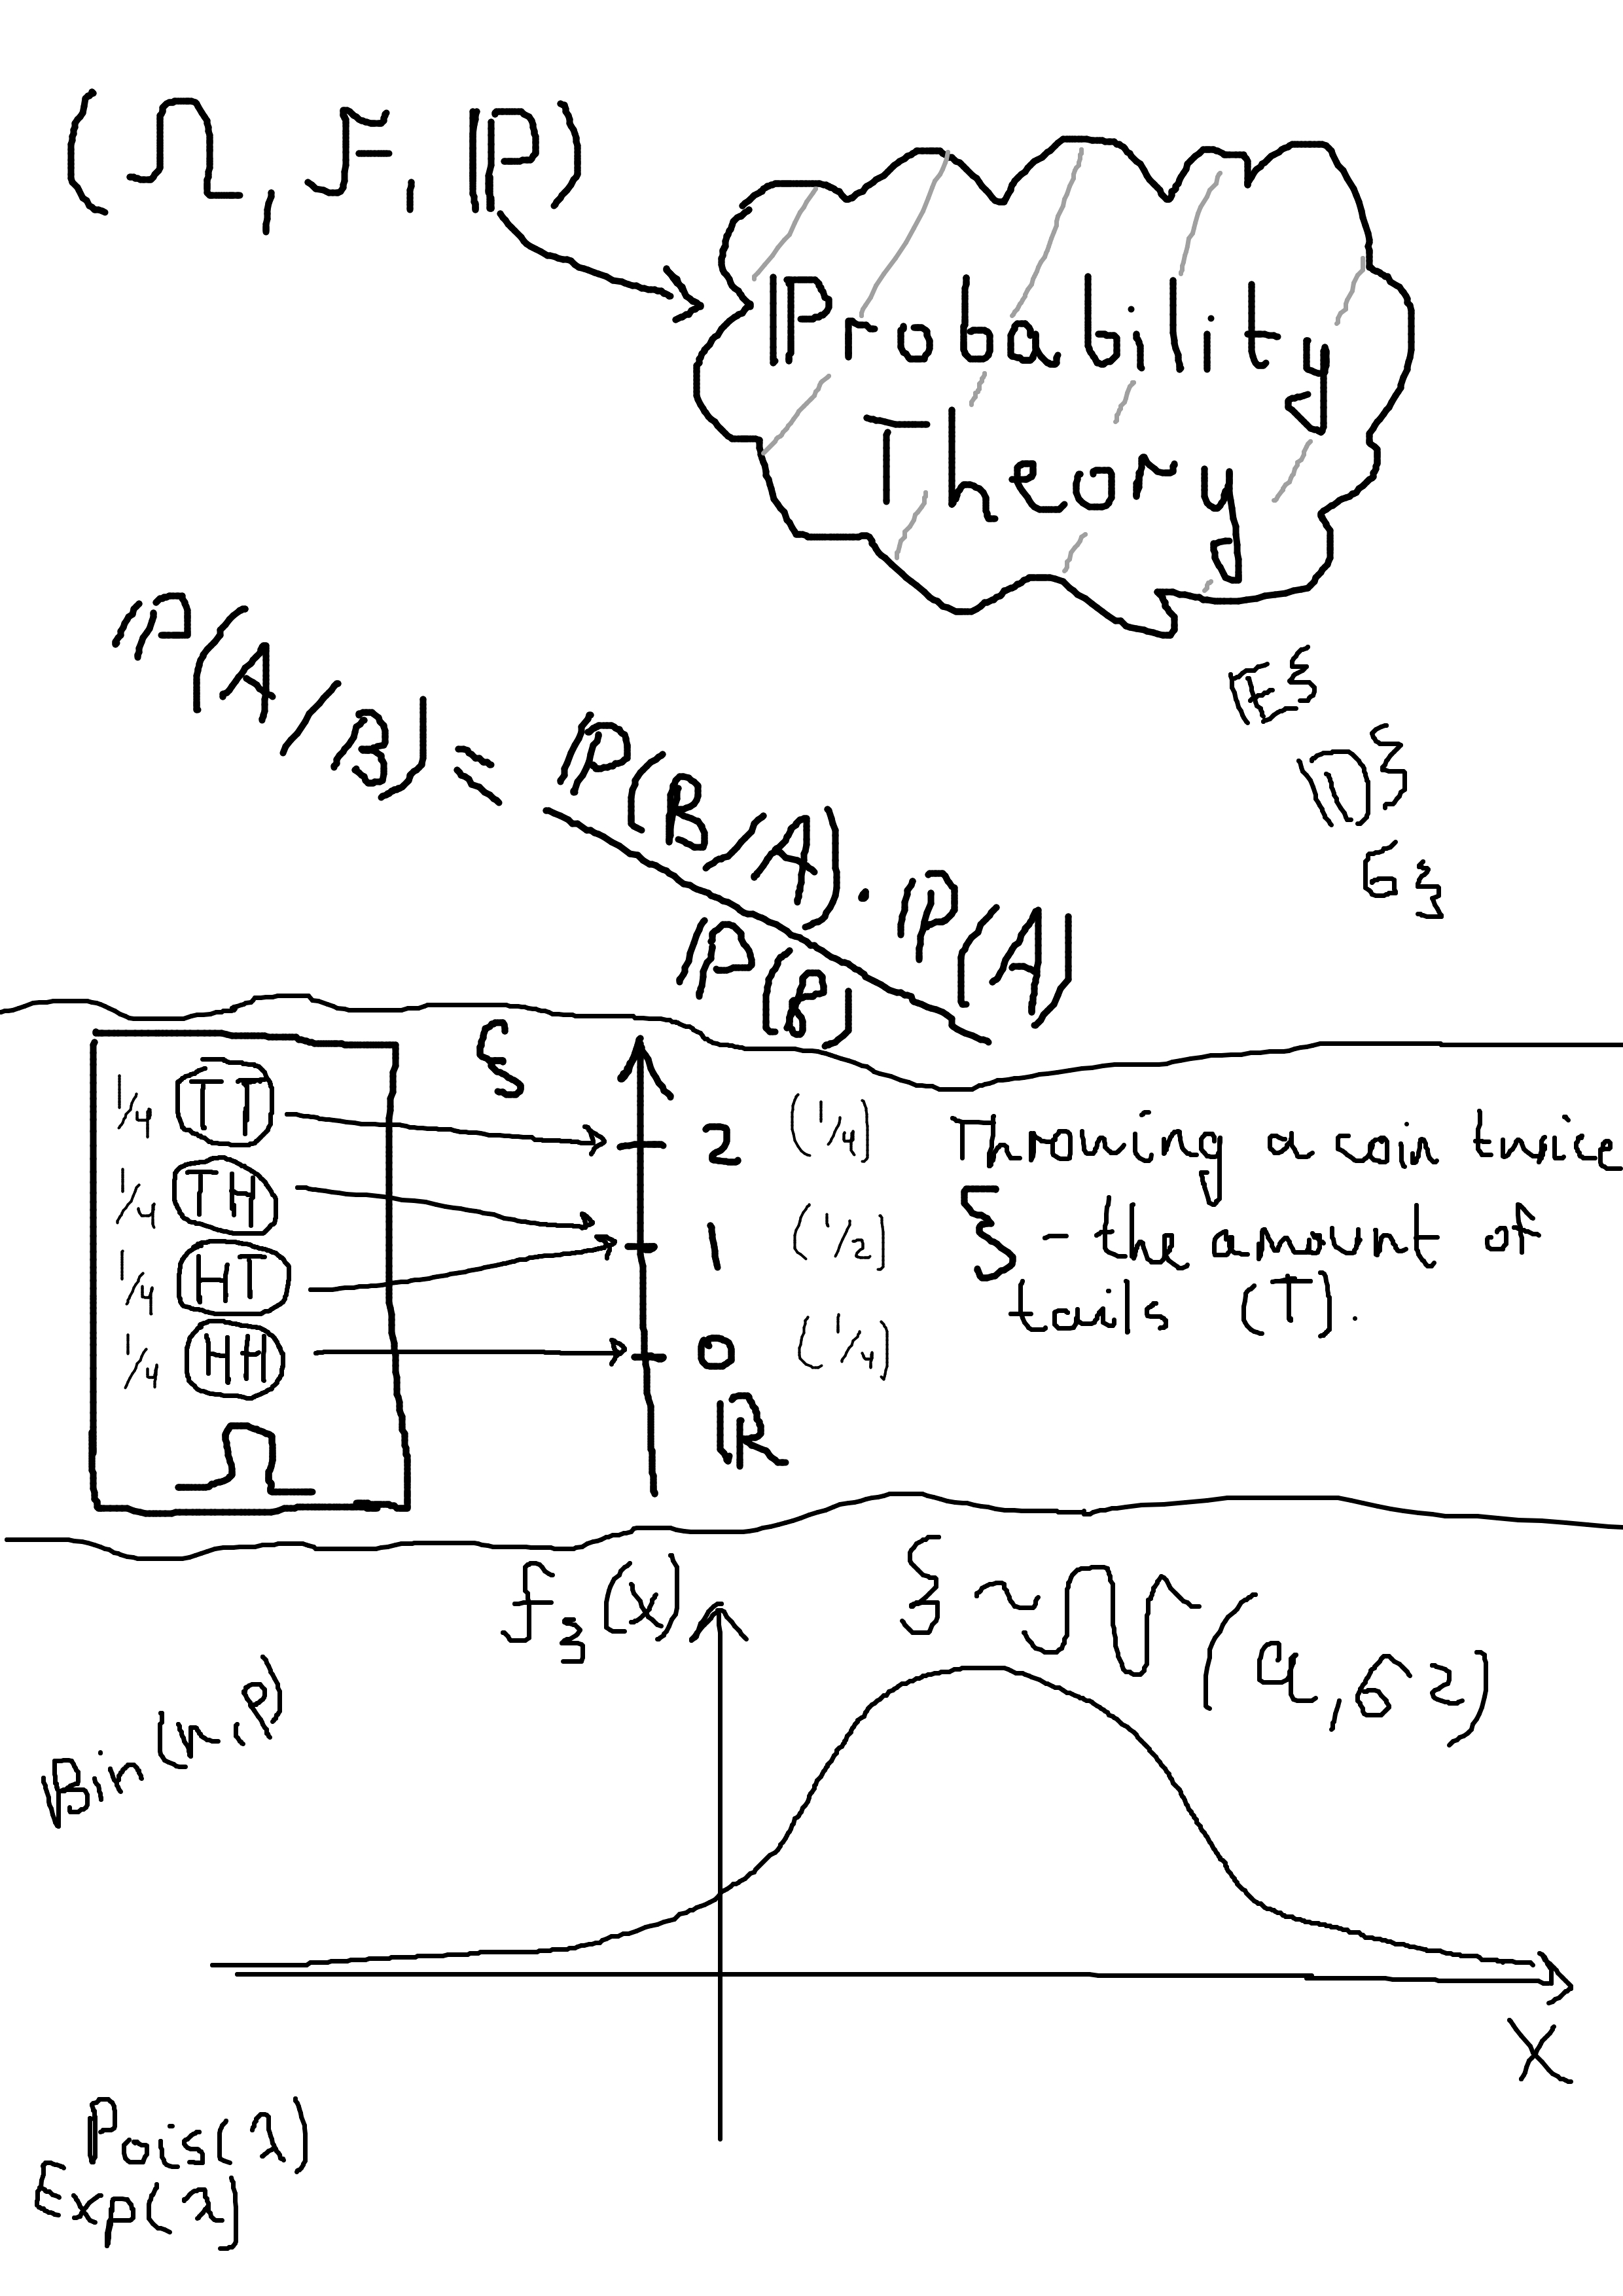
\includepdf[scale=1]{preview.jpg}

\tableofcontents
\newpage
\section*{Попередні знання, які необхідні}
Перед початком теорії груп наполегливо рекомендується згадати такі предмети:
\begin{itemize}[nosep,wide=0pt]
\item більшу частину теорії дискретної математики, як-от: теорія множин, відношень, трошки про відображення, трошки комбінаторики (останнє опціонально, але не завадить ніколи);
\item більшу частину теорії чисел, зокрема: вся теорія про подільність, теорія про конгруентні числа, базові відомості про функції Ойлера;
\item трошки теорії многочленів (залишив у PDF аналітичної геометрії);
\item частину лінійної алгебри, особливо матриці. Для нормального засвоєння розділу 5 дуже бажано мати відомості про векторні простори.
\end{itemize}
Третє не сильно принципово, оскільки ми покриємо ще раз теорію многочленів уже в загальному представленні. Але просто для простої орієнтації варто пройтися трошки.
\newpage

\section{Теорія груп}
У цьому розділі я почну одразу з означення групи, хоча є деякі корисні терміни: алгебраїчна структура, оператив, моноїд тощо. Але основна мета цього розділу -- суто робота з групами, тому одразу даю більш розгорнуте означення.

\subsection{Означення груп}
\begin{definition}
Задана $G$ -- деяка множина, $*$ -- деяка бінарна операція.\\
\textbf{Групою} назвемо пару $\left<G, *\right>$, для якої виконуються такі властивості:\\
I. Замкненість відносно операції:
\begin{align*}
\forall a,b \in G: a*b \in G
\end{align*}
II. Підпорядкована такими аксіомами:
\begin{align*}
\begin{tabular}{lll}
1) & $\forall a,b,c \in G: a*(b*c) = (a*b)*c$ & -- асоціативність \\
2) & $\exists e \in G: a*e = e*a = a$ & -- існування нейтрального елементу \\
3) & $\forall a \in G: \exists a^{-1} \in G: a*a^{-1} = a^{-1}*a = e$ & -- існування оберненого елементу
\end{tabular}
\end{align*}
\end{definition}

\begin{example}
Розглянемо ось такі приклади груп:
\begin{figure}[H]
\centering
\begin{tabular}{c|c|c|c|c}
$G$ & $*$ & $e$ & $a$ & $a^{-1}$ \\
\hline
$\mathbb{Z}$ & $+$ & $0$ & $n$ & $-n$ \\
$\mathbb{R} \setminus \{0\}$ & $\cdot$ & $1$ & $r$ & $\dfrac{1}{r}$ \\
$\Mat_{n \times n}(\mathbb{R})$ & $+$ & $O$ & $A$ & $-A$ \\
$\{-1,1\}$ & $\cdot$ & $1$ & $1,-1$ & $1,-1$
\end{tabular}
\end{figure}
\end{example}

\begin{example}
Ось така струткура $\left< \Mat_{n \times n}(\mathbb{R}, \cdot \right>$ уже не буде групою. Тому що для не для всіх матриц $A \in \Mat_{n \times n}$ існує оберненої матриці $A^{-1}$. Якщо $\det A = 0$, то нема оберненої.
\end{example}

\begin{example}
Але тепер розглянемо $\left< GL_n, \cdot \right>$, де $GL_n$ (general linear group) -- множина матриць з $\Mat_{n \times n}(\mathbb{R})$ з ненульовими визначниками. Доведемо, що це утворює групу.\\
I. Нехай $A,B \in GL_n$, тобто $\det A \neq 0,\ \det B \neq 0$. Тоді звідси випливає, що $\det (AB) = \det A \cdot \det B \neq 0$, а тому звідси $AB \in GL_n$.\\
II. Перевіримо три аксіоми:\\
1) Нехай $A,B,C \in GL_n$, тоді звідси $A \cdot (B \cdot C) = (A \cdot B) \cdot C$ (асоціативність кожних трьох матриць виконується із теорії матриць лінійної алгебри).\\
2) Існує матриця $I$ -- одинична матриця, причому $\det I = 1 \neq 0$, а тому $I \in GL_n$ та $A \cdot I = I \cdot A = A$.\\
3) Нехай $A \in GL_n$, тобто $\det A \neq 0$. Значить, існує $A^{-1} = \dfrac{1}{\det A} \overline{A}$, де $\overline{A}$ -- приєднана матриця, для якої $A \cdot A^{-1} = A^{-1} \cdot A = I$.
\end{example}

\begin{proposition}
Задана $\left<G,* \right>$ -- група. Тоді виконуються такі пункти:
\begin{enumerate}[nosep,wide=0pt, label={\arabic*)}]
\item існуючий нейтральний елемент $e \in G$ -- єдиний;
\item для кожного елемента $a \in G$ обернений елемент $a^{-1} \in G$ -- єдиний.
\end{enumerate}
\end{proposition}

\begin{proof}
Покажемо виконання кожного пункту від супротивного.
\begin{enumerate}[wide=0pt,label={\arabic*)}]
\item !Припустимо, що існують два нейтральних елементи: $e_1,e_2 \in G$. Отримаємо такий ланцюг рівностей:\\
$e_1 = e_1*e_2$ та $e_2 = e_1*e_2$, а тому звідси $e_1 = e_2$.

\item !Припустимо, що для $a \in G$ існують два обернени $a_1^{-1},a_2^{-1} \in G$. Отримаємо такий ланцюг рівностей:\\
$a_1^{-1} = a_1^{-1} * e = a_1^{-1} * (a*a_2^{-1}) = (a_1^{-1}*a)*a_2^{-1} = e*a_2^{-1} = a_2^{-1}$.
\end{enumerate}
У двох випадках отримали суперечність!
\end{proof}

\begin{definition}
Задано $\left< G, * \right>$ -- група та $a \in G$. Нехай $n \in \mathbb{Z}$.\\
\textbf{Степенем елемента} $a$ назвемо наступне:
\begin{align*}
a^n = \underbrace{a*a*\dots*a}_{n \text{ разів}} \\
a^{-n} = (a^{-1})^{n} \\
a^0 = e
\end{align*}
\end{definition}

\begin{proposition}[Властивості]
Задана $\left<G, *\right>$ -- група. Тоді виконуються наступне:
\begin{enumerate}[nosep, wide=0pt, label={\arabic*)}]
\item рівняння $a*x = b$ має єдиний розв'язок $x=a^{-1}*b$;
\item $a*x = b*x \iff a = b$ (тобто виконується скорочення);
\item $(a*b)^{-1} = b^{-1}*a^{-1}$;
\iffalse\textit{Аналогічно для $x*a=b$ та $x*a=x*b$ виконано}.\fi
\item $a^{n+m} = a^n*a^m$;
\item $(a^n)^m = a^{nm}$.
\end{enumerate}
\textit{Доведення нескладні.}
\end{proposition}

\begin{definition}
Задано $\left<G,* \right>$ -- група.\\
Вона називається \textbf{абелевою}, якщо
\begin{align*}
\forall a,b \in G: a*b = b*a \text{ -- комутативність}
\end{align*}
\end{definition}

\begin{example}
Зокрема $\left< \mathbb{Z},+ \right>$, $\left< \mathbb{R} \setminus \{0\}, \cdot \right>$, $\left< \{-1,1\}, \cdot \right>$ -- абелеві групи.
\end{example}

\subsection{Деякі інші корисні групи}
\subsubsection{Групи класів лишків}
Розглянемо множину $\mathbb{Z}$ та будь-яке натуральне число $p \in \mathbb{N}$. Задамо відношення еківалентності:
\begin{align*}
x \sim y \iff x \equiv y \pmod p
\end{align*}
Ми вже її якось встигли профакторизувати ось так (див. дискретку):\\
$\mathbb{Z}/_{\!\!\pmod p} = \{[0],\ [1],\ \dots,\ [p-1] \}$, де\\
$[0] = \{\dots,-2p,-p,0,p,2p,\dots\}$\\
$[1] = \{\dots, -2p+1,-p+1,1,p+1,2p+1,\dots\}$\\
$\vdots$\\
$[p-1] = \{-p-1,-1,p-1,2p-1,3p-1),\dots\}$.
\bigskip \\
Зробимо перепозначення $[k] = \overline{k}$, а також $\mathbb{Z}/_{\!\!\pmod p} = \mathbb{Z}_p$.
\begin{definition}
Отримана фактормножина
\begin{align*}
\mathbb{Z}_p = \{\overline{0}, \overline{1}, \dots, \overline{p-1} \} \\
\overline{k} = \{\dots,-2p+k,-p+k,k,p+k,2p+k,\dots\}
\end{align*}
називається \textbf{класом лишків} за модулем $p$.
\end{definition}

\begin{figure}[H]
\centering
\begin{tikzpicture}
\draw[dashed, black!30] (-1,-1.5) rectangle (7,1.5) node[scale=0.8, black] at (-0.8,1.3) {$\mathbb{Z}$};
\draw[dashed, black!30] (1.5,-1.5)--(1.5,1.5);
\draw[dashed, black!30] (4.5,-1.5)--(4.5,1.5);

\node[red] at (0,0) {$0$};
\node[red] at (0.5,0.5) {$-3$};
\node[red] at (0.7,-0.1) {$3$};
\node[red] at (0.1,-0.5) {$-6$};
\node[red] at (-0.5,-0.2) {$9$};
\node[red] at (-0.2,0.6) {$6$};
\node at (0,-1) {$\vdots$};
\node at (0,-2.2) {$\overline{0}$};
%0

\node[green] at (3,0) {$1$};
\node[green] at (3.5,0.5) {$-4$};
\node[green] at (3.7,-0.1) {$4$};
\node[green] at (3.1,-0.5) {$-7$};
\node[green] at (2.5,-0.2) {$11$};
\node[green] at (2.8,0.6) {$7$};
\node at (3,-1) {$\vdots$};
\node at (3,-2.2) {$\overline{1}$};
%1

\node[blue] at (6,0) {$2$};
\node[blue] at (6.5,0.5) {$-5$};
\node[blue] at (6.7,-0.1) {$5$};
\node[blue] at (6.1,-0.5) {$-8$};
\node[blue] at (5.5,-0.2) {$12$};
\node[blue] at (5.8,0.6) {$8$};
\node at (6,-1) {$\vdots$};
\node at (6,-2.2) {$\overline{2}$};
%2
\end{tikzpicture}
\caption*{На прикладі проілюстрував множину $\mathbb{Z}_3 = \{ \overline{0}, \overline{1}, \overline{2} \}$.}
\end{figure}

\begin{theorem}
$\left<\mathbb{Z}_p, + \right>$ -- абелева група, де операція визначається таким чином: $\overline{a}+\overline{b} \eqbydef \overline{a+b}$.
\end{theorem}

\begin{proof}
Для початку треба з'ясувати, чи є коректно визначеною операція.\\
Тобто нехай $\overline{a} = \overline{c}$ та $\overline{b} = \overline{d}$. Хочемо довести, що $\overline{a+b} = \overline{c+d}$.\\
%Паралель: 1/2 = 2/4 та 1/3 = 3/6, тоді треба пересвідчитись, що 1/2+1/3 = 5/6 - це той самий елемент, що й 2/4 + 3/6 = 10/12
Маємо $a \equiv c \pmod p$ та $b \equiv d \pmod p$. А тому за властивостями конгруенції (див. теорію чисел), $a+b \equiv c+d \pmod p$. Тобто $\overline{a+b} = \overline{c+d}$.
\iffalse
Перш за все необхідно показати, що визначена операція коректна.
\begin{example}
На конкретному прикладі візьмемо множину $\mathbb{Z}_5$.\\
Ми хочемо, щоб $\overline{1} + \overline{2} = \overline{3}$. Для коректної рівності нам необхідно, щоб кожний елемент з $\overline{1}$ плюс кожний елемент з $\overline{2}$ обов'язково став елементом, що завжди потрапить в $\overline{3}$. Якщо тут розписати множині один за одним, то там все виконується на око.\\
Математично кажучи, $\begin{cases} x \in \overline{m} \\ y \in \overline{n} \end{cases} \implies x+y \in \overline{m+n}$.\\
Перефразувавши: $\begin{cases} x \equiv m \pmod p \\ y \equiv n \pmod p \end{cases} \implies x+y \equiv m+n \pmod p$.
\end{example}
Насправді кажучи, це властивість з теорії чисел про дільність за модулем, тому все в нас коректно визначено.
\fi
\bigskip \\
А тепер час довести, що це абелева -- група.\\
I. $\overline{a},\ \overline{b} \in \mathbb{Z}_p: \overline{a}+\overline{b} = \overline{a+b} \in \mathbb{Z}_p$ -- тобто замкненість є, бо отримали, по суті, клас еквівалентності.\\
II. Перевіримо аксіоми груп.\\
1) $\forall \overline{a},\ \overline{b},\ \overline{c} \in \mathbb{Z}_p: \overline{a}+(\overline{b}+\overline{c}) = \overline{a}+\overline{b+c} = \overline{a+(b+c)} = \overline{(a+b)+c} = \overline{a+b} + \overline{c} = (\overline{a}+\overline{b})+\overline{c}$ -- тобто асоціативність є.\\
2) нейтральним елементом стане $\overline{0} \in \mathbb{Z}_p$, тому що $\overline{a} + \overline{0} = \overline{a+0} = \overline{a}$.\\
3) для $\overline{a} \in \mathbb{Z}_p$ оберненим елементом стане $\overline{a}^{-1} = \overline{p-a}$, бо $\overline{a} + \overline{a}^{-1} = \overline{a} + \overline{p-a} = \overline{a+p-a} = \overline{p} = \overline{0}$.\\
Для абелевої групи треба довести комутативність. Справді,\\
$\forall \overline{a},\overline{b} \in \mathbb{Z}_p: \overline{a} + \overline{b} = \overline{a+b} = \overline{b+a} = \overline{b} + \overline{a}$ -- тобто комутативність є.
\end{proof}

\begin{example}
Є ще така штука як \textbf{таблиця Келі}, покажу на прикладі $\left<\mathbb{Z}_3,+ \right>$.
\begin{figure}[H]
\centering
\begin{tabular}{c|ccc}
$+$ & $\overline{0}$ & $\overline{1}$ & $\overline{2}$ \\
\hline
$\overline{0}$ & $\overline{0}$ & $\overline{1}$ & $\overline{2}$ \\
$\overline{1}$ & $\overline{1}$ & $\overline{2}$ & $\overline{0}$ \\
$\overline{2}$ & $\overline{2}$ & $\overline{0}$ & $\overline{1}$ \\
\end{tabular}
\end{figure}
Фактично кажучи, в таблиці Келі описуються всі можливі (у цьому випадку) додавання між двома об'єктами та їхні результати.
\end{example}

\begin{theorem}
\label{multiplicative_class_of_residues_mod_n_is_a_group}
$\left< \mathbb{Z}_p \setminus \{\overline{0}\}, \cdot \right>$, де $p$ -- просте число -- абелева група, де операція визначається таким чином: $\overline{a} \cdot \overline{b} \overset{\text{def.}}{=} \overline{a \cdot b}$.
\end{theorem}

\begin{remark}
Можна зауважити два обмеження: вилучення елемента $\overline{0}$ та необідність $p$ бути простим. Обґрунтую обмеження прикладами.
\end{remark}

\begin{example}
Маємо структуру $\left< \mathbb{Z}_p, \cdot \right>$, яка не буде групою, тому що нема нейтрального елемента.\\
!Припустімо, що $\overline{e} \in \mathbb{Z}_p$ -- це нейтральний елемент, тобто \\ $\forall \overline{a} \in \mathbb{Z}_p: \overline{a} \cdot \overline{e} = \overline{a}$. Звідси випливає, що $\overline{e} = \overline{1}$.\\
Водночас $\overline{0} = \overline{0} \cdot \overline{1} = \overline{1}$. Суперечність!
\end{example}

\begin{example}
Тепер маємо структуру $\left<\mathbb{Z}_p \setminus \{\overline{0}\}, \cdot \right>$, де $p$ -- складене. Уже нейтральний елемент існує, утім все одно не буде групою.\\
Оскільки $p$ -- складене, то існує якийсь інший дільник $n \neq p, n \neq 1$. Тому звідси $p = nm \implies \overline{p} = \overline{n} \cdot \overline{m}$.\\
Але $\overline{p} = \overline{0}$, а тому $\overline{n}\cdot \overline{m} = \overline{0}$. А це означає, що хоча $\overline{m}, \overline{n} \in \mathbb{Z}_p$, але $\overline{mn} = \overline{0} \not\in \mathbb{Z}_p$. Замкненості нема.
\end{example}

Тепер повернімося до нашої теореми та проведемо її доведення.
\begin{proof}
I. Доведемо, що $\forall \overline{a},\ \overline{b} \in \mathbb{Z}_p \setminus \{ \overline{0}\}: \overline{a} \cdot \overline{b} \in \mathbb{Z}_p \setminus \{ \overline{0}\}$.\\
!Припустимо, що $\overline{a} \cdot \overline{b} \not\in \mathbb{Z}_p \setminus \{ \overline{0}\}$, тоді єдиний варіант -- це $\overline{a} \overline{b} = \overline{ab} = \overline{0}$, тобто $p \mid ab$. А оскільки $p$ -- просте, то звідси або $p \mid a$, або $p \mid b$. У двох випадках отримаємо суперечність!\\
Отже, замкненість перевірена успішно.
\bigskip \\
II. Тепер доведемо виконання аксіом груп.\\
1) $\forall \overline{a},\ \overline{b},\ \overline{c} \in \mathbb{Z}_p \setminus \{ \overline{0}\}: \overline{a}(\overline{b}\overline{c}) = \overline{a}\overline{bc} = \overline{a(bc)} = \overline{(ab)c} = \overline{ab} \overline{c} = (\overline{a}\overline{b})\overline{c}$ -- тобто асоціативність є;\\
2) нейтральним елементом стане $\overline{1} \in \mathbb{Z}_p \setminus \{ \overline{0}\}$, тому що $\overline{a} \overline{1} = \overline{a \cdot 1} = \overline{a}$;\\
3) а ось з оберненим елементом ситуація складніша. Маємо $\overline{a} \in \mathbb{Z}_p \setminus \{ \overline{0}\}$, розглянемо ось таку множину: $\{\overline{a}, \overline{2a}, \dots, \overline{(p-1)a} \}$. Спочатку покажемо, що тут всі елементи абсолютно різні. \\
!Припускаючи, що $\overline{k_1 a} = \overline{k_2 a}$ для $k_1 \neq k_2$, ми отримаємо $k_1 a \equiv k_2 a \pmod p \implies (k_1-k_2)a \equiv 0 \pmod p$. У силу того, що $p$ -- просте, то або $p \mid a$, що точно неправда, або $p \mid k_1-k_2$. Але це має місце лише тоді, коли $k_1 = k_2$, оскільки $k_1,k_2 = \overline{1,p-1}$. Суперечність!\\
Отже, множина $\{\overline{a}, \overline{2a}, \dots, \overline{(p-1)a} \}$ містить різні елементи. Так само різні елементи містить $\mathbb{Z}_p \setminus \{ \overline{0}\}$, тобто фактично ми отримали, що\\
$\{\overline{a}, \overline{2a}, \dots, \overline{(p-1)a} \} = \{ \overline{1}, \overline{2}, \dots, \overline{p-1} \} = \mathbb{Z}_p \setminus \{ \overline{0}\}$.\\
Таким чином, елемент серед елементів $\overline{ka}$, де $k = 1,2,\dots,p-1$, має бути елемент $\overline{1}$. \\
Тоді для $\overline{a} \in \mathbb{Z}_p \setminus \{ \overline{0}\}$ знайдеться деякий $\overline{ka}$, для якого $\overline{ka} = \overline{k} \overline{a} = \overline{1}$, і от $\overline{k}$ буде деяким оберненим елементом.\\
Залишилось показати, що це абелева група. Справді,\\
$\forall \overline{a},\ \overline{b} \in \mathbb{Z}_p \setminus \{ \overline{0}\}: \overline{a} \overline{b} = \overline{ab} = \overline{ba} = \overline{b} \overline{a}$ -- тобто комутативність є.
\end{proof}

\begin{example}
Тут теж будується \textbf{таблиця Келі}, покажу на $\left<\mathbb{Z}_5 \setminus \{\overline{0}\},\cdot \right>$.
\begin{figure}[H]
\centering
\begin{tabular}{c|cccc}
$\cdot$ & $\overline{1}$ & $\overline{2}$ & $\overline{3}$ & $\overline{4}$ \\
\hline
$\overline{1}$ & $\overline{1}$ & $\overline{2}$ & $\overline{3}$ & $\overline{4}$ \\
$\overline{2}$ & $\overline{2}$ & $\overline{4}$ & $\overline{1}$ & $\overline{3}$ \\
$\overline{3}$ & $\overline{3}$ & $\overline{2}$ & $\overline{4}$ & $\overline{2}$ \\
$\overline{4}$ & $\overline{4}$ & $\overline{3}$ & $\overline{2}$ & $\overline{1}$ \\
\end{tabular}
\end{figure}
Фактично тут описується всі можливі множення між двома об'єктами та їхні результати. І ось тут таблиця Келі має сенс, тому що під час доведення ми не знайшли явної формули знаходження оберненого елементу, тому варто будувати табличку.
\end{example}

Але все ж таки повернімось назад до структури $\left< \mathbb{Z}_n \setminus \{\overline{0}\}, \cdot \right>$, де $n \in \mathbb{N}$, що вже має нейтральний елемент $\overline{e} = \overline{1}$.

\begin{lemma}
$\overline{m} \in \mathbb{Z}_n \setminus \{ \overline{0} \}$ має обернений елемент $\iff \gcd(m,n) = 1$.
\end{lemma}

\begin{proof}
\rightproof Дано: $\overline{m} \in \mathbb{Z}_n \{\overline{0}\}$ має обернений, тобто $\exists \overline{x} \in \mathbb{Z}_n \setminus \{\overline{0}\}: \overline{m} \cdot \overline{x} = \overline{1}$.\\
Тобто $mx \equiv 1 \pmod n$ для деякого $x$. Із курсу теорії чисел, можемо сказати, що $\gcd(m,n) \mid 1 \implies \gcd(m,n) = 1$.
\bigskip \\
\leftproof Дано: $\gcd(m,n) = 1$, тоді рівняння $mx \equiv 1 \pmod n$ матиме єдиний розв'язок $x$, із курсу теорії чисел. Мовою класів лишків, маємо \\ $\overline{mx} = \overline{m} \cdot \overline{x} = \overline{1}$. Таким чином, $\overline{m} \in \mathbb{Z}_n$ має обернений.
\end{proof}

Познайомимось з ось такою множиною:
$$ U_n = \{ \overline{m} \in \mathbb{Z}_n | \gcd(m,n) = 1 \}$$

\begin{example}
Зокрема маємо $U_9 = \{\overline{1},\overline{2},\overline{4},\overline{5},\overline{7},\overline{8} \}$.
\end{example}

\begin{theorem}
$\left<U_n, \cdot \right>$ -- абелева група з операцією $\cdot$ як було в $\mathbb{Z}_n \setminus \{ \overline{0} \}$.
\end{theorem}

\begin{proof}
I. Із теорії чисел, відомо, що $\begin{cases} \gcd(a,n) = 1 \\ \gcd(b,n) = 1 \end{cases} \implies \gcd(ab,n) = 1$. А тому звідси $\forall \overline{a},\ \overline{b} \in U_n: \overline{ab} \in U_n$.\\
II. Комутативність, асоціативність аналогічно доводиться, як і в минулій теоремі. Нейтральний елемент досі $\overline{e} = \overline{1}$. Кожний елемент має обернений, бо $\overline{m} \in U_n \implies \gcd(m,n) = 1$. Тут спрацьовує лема.
\end{proof}

\subsubsection{Діедральні групи}
\begin{definition}
\textbf{Дієдральною групою} називають групу симетрій правильного $n$-кутника.\\
Позначення: $D_n$ (інколи $D_{2n}$).
\end{definition}

Розглянемо правильний $n$-кутник.
\begin{figure}[H]
\centering
\begin{tikzpicture}
   \newdimen\R
   \R=2cm
   \draw (0:\R) \foreach \x in {60,120,...,360} {  -- (\x:\R) };
   \foreach \x/\l/\p in
     { 60/{1}/above,
      120/{2}/above,
      180/{$\vdots$}/left,
      240/{$n-2$}/below,
      300/{$n-1$}/below,
      360/{$n$}/right
     }
     \node[inner sep=1pt,circle,draw,fill,label={\p:\l}] at (\x:\R) {};
\end{tikzpicture}
\end{figure}
Над цією фігурою робитемо два перетворення (це всі симетрії):\\
1) обертання відносно центра фігури проти годинникової стрілки;\\
2) відбиття відносно осі, що проходить через центр фігури.
\bigskip \\
Зауважимо, що в цьому випадку $\card D_{n} = 2n$.\\
Щоб кожну вершину зсунути проти годинниковою стрілкою, треба на $n$-кутник застоувати обертання розміром $\dfrac{360^\circ}{n}$. Цю дію позначимо за $r$.
\begin{figure}[H]
\centering
\begin{tikzpicture}
   \newdimen\R
   \R=2cm
   \draw (0:\R) \foreach \x in {60,120,...,360} {  -- (\x:\R) };
   \foreach \x/\l/\p in
     { 60/{1}/above,
      120/{2}/above,
      180/{$\vdots$}/left,
      240/{$n-2$}/below,
      300/{$n-1$}/below,
      360/{$n$}/right
     }
     \node[inner sep=1pt,circle,draw,fill,label={\p:\l}] at (\x:\R) {};
     
     \draw[->] (4,0)--(5,0) node[anchor = south east] {$r$};
\end{tikzpicture}
\qquad
\begin{tikzpicture}
   \newdimen\R
   \R=2cm
   \draw (0:\R) \foreach \x in {60,120,...,360} {  -- (\x:\R) };
   \foreach \x/\l/\p in
     { 60/{$n$}/above,
      120/{1}/above,
      180/{2}/left,
      240/{$\ddots$}/below,
      300/{$n-2$}/below,
      360/{$n-1$}/right
     }
     \node[inner sep=1pt,circle,draw,fill,label={\p:\l}] at (\x:\R) {};
\end{tikzpicture}
\end{figure}
$r^k$ -- означає $k$ разів застосувати обертання.\\
Ясно, що $r^n = e$ -- повернемось до початкового положення.
\bigskip \\
Для правильних $n$-кутників всього рівно $n$ вісів симетрій. Візьмемо якусь одну вісь та зробимо відбиття. Цю дію позначимо за $s$.
\begin{figure}[H]
\centering
\begin{tikzpicture}
   \newdimen\R
   \R=2cm
   \draw (0:\R) \foreach \x in {60,120,...,360} {  -- (\x:\R) };
   \foreach \x/\l/\p in
     { 60/{1}/above,
      120/{2}/above,
      180/{$\vdots$}/left,
      240/{$n-2$}/below,
      300/{$n-1$}/below,
      360/{$n$}/right
     }
     \node[inner sep=1pt,circle,draw,fill,label={\p:\l}] at (\x:\R) {};
     \draw[dashed] (0,-2.2)--(0,2.2);
     
     \draw[->] (4,0)--(5,0) node[anchor = south east] {$s$};
\end{tikzpicture}
\qquad
\begin{tikzpicture}
   \newdimen\R
   \R=2cm
   \draw (0:\R) \foreach \x in {60,120,...,360} {  -- (\x:\R) };
   \foreach \x/\l/\p in
     { 60/{2}/above,
      120/{1}/above,
      180/{$n$}/left,
      240/{$n-1$}/below,
      300/{$n-2$}/below,
      360/{$\vdots$}/right
     }
     \node[inner sep=1pt,circle,draw,fill,label={\p:\l}] at (\x:\R) {};
\end{tikzpicture}
\end{figure}
Ясно, що $s^2 = e$ -- повернемось до початкового положення.
Інші $n-1$ відбиття, які є в $n$-кутнику, виражаються через обраний вісь відбиття $s$ та певну кількість обертань $r$, тобто маємо:\\
$s,rs,r^2s,\dots, r^{n-1}s$.\\
Чому ці відбиття різні, тому що якби $r^k s = r^l s$, то було б обов'язоко $r^k = r^l$, що неможливо при $k \neq l$.\\
Також жодне з цих перетворень не є обертанням (тобто це дійсно відбиття), бо якби $r^l = r^ks$, то було б $s = r^{l-k}$, що неможливо. Адже симетрія змінює орієнтацію, а обертання -- ні.\\
Із цих міркувань ми робимо висновок, що нам неважливо, який вісь відбиття треба брати.\\
Ще хочеться зауважити, що $rs = sr^{n-1}$, це теж саме, що $rs rs = e$. Уже було з'ясовано, що $rs$ буде відбиттям, а тому звідси $(rs)^2 = e$.\\
\iffalse Зауважимо також, що $rs = sr^{n-1}$.\\
А за МІ можна довести, що $r^m s = s r^{n-m}$.\fi

Таким чином, ми отримаємо вид дієдральної групи:
\begin{align*}
D_n = \{ \underbrace{e,r,r^2,\dots,r^{n-1}}_{\text{обертання}}, \underbrace{s,rs,r^2s,\dots,r^{n-1}s}_{\text{відбиття}} \},
\end{align*}
де $r^n = e,\ s^2 = e,\ rs = sr^{n-1}$.\\
Можна ще переписати це як $D_n = [s,r]$.

\begin{theorem}
$\left< D_n, \circ \right>$ -- справді група. Тут операція $\circ$ -- композиція дій на $n$-кутник. (явно я це не вказував для зручності)
\end{theorem}

\iffalse
\begin{proof}
Замкненість випливає з виразів $r^n = e, s^2 = e, r^ms = sr^{n-m}$. В останньому виразі ми користуватись властивістю асоціативності. І маємо на це права, бо композиція відображень завжди асоціативна.\\
Нейтральний елемент тут $e$ - нічого не робить з $n$-кутником.\\
Оборотні елементи для $r^k$ маємо $(r^{k})^{-1} = r^{n-k}$; для $r^k s$ маємо $(r^k s)^{-1} = s r^{-k} = s(r^k)^{-1}$.
\end{proof}
\fi

\begin{remark}
$\left< D_n, \circ \right>$ -- не абелева група в загальному випадку.\\
Принаймні тому, що $sr \neq rs$.
\end{remark}

\subsubsection{Групи кватерніонів}
Розглядається ось така множина:
\begin{align*}
Q_8 = \{1,-1,i,-i,j,-j,k,-k\}
\end{align*}
з операцією $\cdot$, яка працює ось таким чином:
\begin{align*}
i^2 = j^2 = k^2 = -1 \\
ijk = -1
\end{align*}
Тут числа $1,-1$ -- природним чином задані, не абстрактно.

\begin{theorem}
$\left<Q_8, \cdot \right>$ -- група.
\end{theorem}

\begin{proof}
На основі заданих правил, можна отримати ще такі співвідношення:\\
$ij = k$ \hspace{1cm} $ji = -k$\\
$jk = i$ \hspace{1cm} $kj = -i$\\
$ki = j$ \hspace{1cm} $ik = -j$\\
Дійсно, \\
$ij = (-ij) (-1) = (-ij) k^2 = -(ijk)k = -(-1)k = k$\\
$ji = ji (1) = ji (-ijk) = -(ji ijk) = -k$.\\
На прикладі першого було пояснення.
\begin{figure}[H]
\centering
\begin{tikzpicture}
\draw[->, thick] (1.1,0.2)--(2,1.8) node at (2,2) {$i$};
\draw[->, thick] (1.6,2)--(0.2,2) node at (-0.2,2) {$j$};
\draw[->, thick] (0,1.8)--(0.9,0.2) node at (1,0) {$k$};
\end{tikzpicture}
\end{figure}
Із цього випливає замкненість операції множення.\\
Покажемо асоціативність, тобто $x(yz) = (xy)z$.\\
Не втрачаючи загальності, припустимо $x = i$. Ми будемо розглядати випадки $y,z \in \{i,j,k\}$ -- загалом $9$ варіантів. Із одиницею всередині все зрозуміло, а мінусові не беремо, бо все те саме з точністю до знака. Якщо всі варіанти розписати, то можна переконатись в рівностях.\\
Нейтральним елеемнтом буде $1$.\\
Залишились обернені елементи:
\begin{figure}[H]
\centering
\begin{tabular}{c|c}
$a$ & $a^{-1}$ \\
\hline
$\pm 1$ & $\pm 1$ \\
$i$ & $-i$ \\
$j$ & $-j$ \\
$k$ & $-k$
\end{tabular}
\end{figure}
Доведено.
\end{proof}

\subsubsection{Симетричні групи}
\begin{definition}
\textbf{Перестановкою} елементів множини $X \neq \emptyset$ називають бієкцію 
\begin{align*}
\sigma \colon X \to X
\end{align*}
\end{definition}
Позначення: $S_X$ -- множина всіх перестановок на множині $X$.

\begin{theorem}
$\left< S_X, \circ \right>$ -- група, якщо $X \neq \emptyset$.
\end{theorem}

Спочатку наведемо кілька важливих лем.

\begin{lemma}
Задано $\sigma, \mu: X \to X$ -- бієкції. Тоді $\sigma \circ \mu$ -- бієкція.\\
Таким чином, це доводить замкненіть. Тобто $\sigma,\mu \in S_X \implies \sigma \circ \mu \in S_X$.
\end{lemma}

\begin{proof}
!Припустимо маємо $a \neq b$, але $\sigma \circ \mu (a) = \sigma \circ \mu (b)$. Тобто звідси $\sigma (\mu(a)) = \sigma (\mu(b)) \implies \mu(a) = \mu(b) \implies a = b$. Суперечність! Довели ін'єктивність.\\
Маємо $u\in X$, тоді $\exists a \in X: \sigma(a) = u$. Водночас для числа $a \in X: \exists k \in X: \mu(k) = a$. Отже, $\sigma \circ \mu (k) = \sigma(\mu(k)) = \sigma(a) = u$. Довели сюр'єкцію.\\
Отже, $\sigma \circ \mu$ -- бієкція.
\end{proof}

\begin{lemma}
Задано $\sigma \colon X \to X$ - бієкція. Тоді існує бієкція $\mu \colon X \to X$, для якого $\sigma(a) = b \iff \mu(b) = a$.\\
Таким чином, це доводить існування оберненого елементу. Тобто для кожного $\sigma \in S_X$ існуватиме $\mu \in S_X$, для якого $\sigma \circ \mu (b) = b, \forall b \in X$ та $\mu \circ \sigma (a) = a, \forall a \in X$.
\end{lemma}

\begin{proof}
Відображення $\mu$ коректно визначено. Дійсно, якщо $\mu(b) = a_1$ та $\mu(b) = a_2$, то отримаємо звідси $\sigma(a_1) = b, \sigma(a_2) = b \implies a_1 = a_2$.\\
!Припустимо, що $b_1 \neq b_2$, але $\mu(b_1) = \mu(b_2)$. Позначимо $a_1 = \mu(b_1), a_2 = \mu(b_2)$. Тоді $b_1 = \sigma(a_1), b_2 = \sigma(a_2)$, а тому $b_1 = \sigma(a_1) = \sigma(a_2) = b_2$. Суперечність! Довели ін'єктивність.\\
Для кожного $a \in X$ існує елемент $b = \sigma(a)$, для якого $\mu(\sigma(a)) = a$. Довели сюр'єктивність.\\
Отже, $\mu$ -- бієкція.
\end{proof}

Далі відомо, що композиція будь-яких відображень -- асоціативна. Нейтральним елементом буде відображення $\id \colon X \to X$, де виконано $\id(x) = x, \forall x \in X$.\\
Останні два міркування та дві вищезгадані леми доводять нашу теорему.

\subsubsection{Групи перестановок}
Один з найпоширеніших симетричних груп -- це група $\left<S_{\{1,2,\dots,n\}}, \circ \right>$, що має ще позначення $\left<S_n, \circ \right>$.\\
Перестановки $\sigma \colon \{1,2,\dots,n\} \to \{1,2,\dots,n\}$ мають ще таке позначення:
$$ \sigma = \begin{pmatrix}
1 & 2 & \dots & n \\
i_1 & i_2 & \dots & i_n
\end{pmatrix},$$
де $\{i_1,i_2,\dots,i_n\}$ -- переставлені числа $\{1,2,\dots,n\}$. Тут $\sigma(k) = i_k$.

\begin{remark}
$\text{card}(S_n) = n!$.
\end{remark}

\begin{example}
Зокрема в групі $\left< S_3, \circ \right>$ маються такі перестановки:\\
$\begin{pmatrix}
1 & 2 & 3 \\
1 & 2 & 3
\end{pmatrix}, \begin{pmatrix}
1 & 2 & 3 \\
1 & 3 & 2
\end{pmatrix}, \begin{pmatrix}
1 & 2 & 3 \\
2 & 1 & 3
\end{pmatrix}, \begin{pmatrix}
1 & 2 & 3 \\
2 & 3 & 1
\end{pmatrix}, \begin{pmatrix}
1 & 2 & 3 \\
3 & 1 & 2
\end{pmatrix}, \begin{pmatrix}
1 & 2 & 3 \\
3 & 2 & 1
\end{pmatrix}$.
\end{example}

Тотожна перестановка виглядає як $\varepsilon = \begin{pmatrix}
1 & 2 & \dots & n \\
1 & 2 & \dots & n
\end{pmatrix}$.\\
Добутком двох перестановок $\sigma,\mu$ називається композиція відображень $\sigma \circ \mu$.

\begin{example}
Наприклад, $\mu = \begin{pmatrix}
1 & 2 & 3 \\
3 & 2 & 1
\end{pmatrix}, \sigma = \begin{pmatrix}
1 & 2 & 3 \\
1 & 3 & 2
\end{pmatrix}$. Тоді\\
$\sigma \circ \mu = \begin{pmatrix}
1 & 2 & 3 \\
1 & 3 & 2
\end{pmatrix} \begin{pmatrix}
1 & 2 & 3 \\
3 & 2 & 1
\end{pmatrix} = \begin{pmatrix}
1 & 2 & 3 \\
2 & 3 & 1
\end{pmatrix}$\\
$\mu \circ \sigma = \begin{pmatrix}
1 & 2 & 3 \\
3 & 2 & 1
\end{pmatrix} \begin{pmatrix}
1 & 2 & 3 \\
1 & 3 & 2
\end{pmatrix} = \begin{pmatrix}
1 & 2 & 3 \\
3 & 1 & 2
\end{pmatrix}$
\end{example}

\begin{example}
Маємо $\sigma = \begin{pmatrix}
1 & 2 & 3 \\
1 & 3 & 2
\end{pmatrix}$. Знайти $\sigma^{-1}$.\\
Оскільки $\sigma$ -- бієкція, при цьому $\sigma(1) = 1, \sigma(2) = 3, \sigma(3) = 2$, тоді $\sigma^{-1}(1) = 1, \sigma^{-1}(3) = 2, \sigma^{-1}(2) = 3$. \\
Такий розв'язок каже нам наступне: ми просто рядки в перестановці $\sigma$ поміняємо місцями, а далі верхній рядок переставимо за порядком. А тому звідси\\
$\sigma^{-1} = \begin{pmatrix}
1 & 3 & 2 \\
1 & 2 & 3
\end{pmatrix} = \begin{pmatrix}
1 & 2 & 3 \\
1 & 3 & 2
\end{pmatrix}$.
\end{example}

\begin{definition}
Задано $\sigma \in S_n$ -- перестановка.\\
Пара $(i_j,i_k)$ називається \textbf{інверсією} перестановки $\sigma$, якщо 
\begin{align*}
\text{при } j < k \text{ маємо  } i_j > i_k
\end{align*}
\end{definition}

\begin{example}
Зокрема для $\sigma = \begin{pmatrix}
1 & 2 & 3 & 4 & 5\\
3 & 2 & 5 & 4 & 1
\end{pmatrix}$ маємо такі інверсії: $(3,2), (3,1), (2,1), (5,4), (5,1), (4,1)$.
\end{example}

\begin{definition}
Перестановка $\sigma \in S_n$ називається \textbf{парною}, якщо
\begin{align*}
\text{кількість інверсії -- парне число.}
\end{align*}
Інакше перестановка називається \textbf{непарною}.\\
\textbf{Парність} перестановки визначається ось так:
\begin{align*}
l(\sigma) = \begin{cases} 1, & \sigma \text{ -- парна}\\ 0, & \sigma \text{ -- непарна} \end{cases}
\end{align*}
\end{definition}

\begin{definition}
Перестановка $\tau \in S_n$ називається \textbf{транспозицією}, якщо лише два елементи змінені місцями, тобто
\begin{align*}
\tau = \begin{pmatrix}
1 & \dots & k & \dots & j & \dots & n \\
1 & \dots & j & \dots & k & \dots & n
\end{pmatrix}
\end{align*}
Особливе позначення: $\tau = (kj)$.
\end{definition}

\begin{lemma}
Задано $\tau$ -- транспозиція. Тоді $\tau^{-1} = \tau$.
\end{lemma}

\begin{proof}
Маємо $\tau = \begin{pmatrix}
1 & \dots & k & \dots & j & \dots & n \\
1 & \dots & j & \dots & k & \dots & n
\end{pmatrix}$.\\
Тобто $\tau(p) = p$ при $p \not\in \{k,j\}$, а тому в силу бієкції маємо $\tau^{-1}(p) = p$.\\
Також $\tau(k) = j, \tau(j) = k$, тоді в силу бієкції $\tau^{-1}(j) = k, \tau^{-1}(k) = j$.\\
Отже, $\tau^{-1} = \begin{pmatrix}
1 & \dots & k & \dots & j & \dots & n \\
1 & \dots & j & \dots & k & \dots & n
\end{pmatrix} = \tau$. \\
Висновок такий, що $\tau^{-1}$ також є транспозицією.
\end{proof}

\begin{theorem}
Будь-яку перестановку $\sigma \in S_n$ можна записати як добуток транспозицій.
\end{theorem}

\begin{remark}
Ящо взяти перестановку $\sigma \in S_n$ та транспозицію $\tau = (jk)$, то звідси $\sigma \circ \tau$ -- та сама перестановка $\sigma$, але елементи на $j,k$ позиціях помінялися місцями. Тобто\\
$\begin{pmatrix}
1 & \dots & j & \dots & k & \dots & n \\
i_1 & \dots & i_j & \dots & i_k & \dots & i_n
\end{pmatrix} \circ \begin{pmatrix}
1 & \dots & j & \dots & k & \dots & n \\
1 & \dots & k & \dots & j & \dots & n
\end{pmatrix} = \begin{pmatrix}
1 & \dots & j & \dots & k & \dots & n \\
i_1 & \dots & i_k & \dots & i_j & \dots & i_n
\end{pmatrix}$
\end{remark}

\begin{proof}
Маємо перестановку $\sigma = \begin{pmatrix}
1 & \dots & n \\
i_1 & \dots & i_n
\end{pmatrix}$. Використовуючи зауваження, ми будемо обирати такі транспозиції, щоб $\{i_1,\dots,i_n\}$ впорядкувати, тобто отримати $\{1,2,\dots,n\}$.\\
Поставимо на місце число $1$. Якщо $i_1 = 1$, то вже стоїть на місці. Інакше якщо $i_1 \neq 1$, то має знайтись інший $i_{k_1} = 1$ при $k_1 \neq 1$. Оберемо транспозицію, що міняє $i_1, i_{k_1}$ місцями, я таку позначу за $\tau_1$, тоді отримаємо $\sigma \circ \tau_1$ -- перестановка, де тепер $1$ стоїть на місці.\\
Аналогічно ставимо число $2$. Якщо $i_2 = 2$, то вже стоїть на місці, а інакше аналогічно беремо відповідну транспозицію -- отримаємо $\sigma \circ \tau_1 \circ \tau_2$, де вже $1,2$ стоять на місцях.\\
$\vdots$\\
І так робимо, допоки не отримаємо ось таку рівність:\\
$\sigma \circ \tau_1 \circ \tau_2 \circ \dots \circ \tau_m = \varepsilon$.\\
Цікаво зазначити, що $m \leq n-1$. Із рівності отримаємо:\\
$\sigma = \tau_1^{-1} \circ \tau_2^{-1} \dots \tau_{m}^{-1} = \tau_1 \circ \tau_2 \dots \circ \tau_m$.\\
Отже, $\sigma$ розклалась в добуток транспозицій. 
\end{proof}

\begin{example}
Зокрема для перестановки $\sigma = \begin{pmatrix}
1 & 2 & 3 & 4 & 5 & 6 \\
5 & 1 & 6 & 4 & 3 & 2
\end{pmatrix}$ маємо таке представлення в добуток транспозицій: $\sigma = (51) \circ (52) \circ (63) \circ (65)$.\\
Це робиться за вищеописаним алгоритмом. Але ніхто не забороняє спочатку поставити на місце останній, потім передостанній і так до першого. Отримаємо іншу репрезентацію:\\
$\sigma = (62) \circ (35) \circ (23) \circ (12)$.\\
А ще ніхто не забороняє зробити ось так:\\
$\sigma = (62) \circ (35) \circ (23) \circ (12) \circ \underbrace{(13) \circ (13)}_{\varepsilon}$.\\
Висновок: розклад на транспозицію не є єдиним.\\
Але вже тут можна зауважити, що всюди однакова парність: парна кількість транспозицій.
\end{example}

\begin{lemma}
Нехай задано $\sigma \in S_n$ -- перестановка та $\tau$ -- довільна транспозиція. Тоді $\sigma$ та $\sigma \circ \tau$ мають різну парність, тобто $l(\sigma) \neq l(\sigma \circ \tau)$.
\end{lemma}

\begin{proof}
$\sigma = \begin{pmatrix}
1 & \dots & k & \dots & j & \dots & n \\
i_1 & \dots & i_k & \dots & i_j & \dots & i_n
\end{pmatrix}$ \hspace{1cm}  $\sigma \circ \tau = \begin{pmatrix}
1 & \dots & k & \dots & j & \dots & n \\
i_1 & \dots & i_j & \dots & i_k & \dots & i_n
\end{pmatrix}$.\\
Візьмемо пару $(i_s,i_t)$ та розглянемо кілька випадків:\\
1. $(i_s,i_t) \neq (i_j,i_k)$. Тоді як і в $\sigma$, так і в $\sigma \circ \tau$ або пара $(i_s,i_t)$ або буде інверсією, або не буде.\\
2. $(i_s,i_t) = \left[ \begin{gathered} (i_s,i_k) \\ (i_s,i_j) \end{gathered} \right.$ при $1 \leq s < k$. Тоді аналогічно або пара $(i_s,i_t)$ або буде інверсією, або не буде.\\
3. $(i_s,i_t) = \left[ \begin{gathered} (i_k,i_t) \\ (i_j,i_t) \end{gathered} \right.$ при $j < t \leq n$ -- абсолютно аналогічно до 2.\\
4. $(і_s,i_t) = (i_k, i_t)$ при $k < t < j$ або $(i_s,i_t) = (i_s,i_j)$ при $k < s < j$. Тоді наочно можна подивитись, що або $(i_s,i_t)$ інверсія $\sigma$ та не інверсія в $\tau \circ \sigma$, або навпаки. Кількість таких пар $j-k-1$  кожному випадку.\\
5. $(i_s,i_t) = (i_k,i_j)$. Очевидно, що або $(i_s,i_t)$ інверсія $\sigma$ та не інверсія в $\tau \circ \sigma$, або навпаки.\\
Остаточно, всього $2 \cdot (j-k-1) + 1$ пар з різною інверсійністю. Цього цілком достатньо, щоб сказати, що $l(\sigma) \neq l(\tau \circ \sigma)$.
\end{proof}

\begin{corollary}
Перестановка $\sigma \in S_n$ -- парна $\iff$ кількість транспозицій в розкладі -- парна.
\end{corollary}

\begin{corollary}
Якщо $\sigma = \sigma_1 \circ \sigma_2$, то тоді $l(\sigma) = l(\sigma_1) \oplus l(\sigma_2)$ (під $\oplus$ мається на увазі сума за модулем $2$).
\end{corollary}

\begin{definition}
Задано $\sigma \in S_n$ -- перестановка.\\
Вона називається \textbf{циклом довжини $k$}, якщо
\begin{align*}
i_1 \mapsto i_2 \mapsto \dots \mapsto i_k \mapsto i_1 \\
x \mapsto x,\ x \neq i_s
\end{align*}
Позначення: $(i_1 i_2 \dots i_k)$.\\
Множину $\{i_1,\dots,i_k\}$ в деякій літературі називають \textbf{носієм} даного цикла.
\end{definition}


\begin{example}
Зокрема перестановка $\sigma = \begin{pmatrix}
1 & 2 & 3 & 4 & 5 \\
1 & 4 & 3 & 5 & 2 
\end{pmatrix}$ буде циклом довжиною $3$, тому що\\
$2 \mapsto 4 \mapsto 5 \mapsto 2$, а також $1 \mapsto 1, 3 \mapsto 3$.\\
Отже, $\sigma = (245)$.
\end{example}

\begin{remark}
Перестановка $\varepsilon = (1)$ також є циклом, але довжини $1$. Усі транспозиції -- цикли довжини $2$.
\end{remark}

\begin{definition}
Задано цикли $(i_1 \dots i_k)$ та $(j_1 \dots j_m)$.\\
Вони називаються \textbf{незалежними}, якщо
\begin{align*}
\{i_1,\dots,i_k\} \cap \{j_1,\dots,j_m\} = \emptyset
\end{align*}
Тобто їхні носії не перетинаються між собою.
\end{definition}

\begin{example}
Зокрема цикли $(23) \in S_6$ та $(456) \in S_6$ -- незалежні.
\end{example}

\begin{lemma}
Задано $\sigma_1, \sigma \in S_n$ -- цикли. Тоді $\sigma_1 \circ \sigma_2 = \sigma_2 \circ \sigma_1$.\\
Тобто цикли комутують між собою.\\
\textit{Вказівка: подивитися наочно.}
\end{lemma}

\begin{theorem}
Будь-яку перестановку $\sigma \in S_n$ можна записати як добуток циклів єдиним чином.
\end{theorem}

\begin{proof}
Маємо перестановку $\sigma \in S_n$. Побудуємо цикл ось таким чином:\\
$1 = i_0 \to \sigma(i_0) \to \sigma^2(i_0) \to \dots \to \sigma^{k_0-1}(i_0) \to \sigma^{k_0}(i_0) = i_0 = 1$.\\
Тут вважаємо, що всі числа до цього різні між собою.\\
Цей цикл обов'язково рано чи пізно почне повторюватись, починаючи з номера $k_0$, просто тому що у нас множина $\{1,2,\dots,n\}$ скінченна.\\
Чи може таке статись, що $\sigma^{k_0}(i_0)$ потрапить в один з $\sigma^{p}(i_0), p = \overline{1,k_0}$ -- ні, не може. Тому що маємо $\sigma^{p-1}(i_0) \mapsto \sigma^p(i_0)$, а якби також $\sigma^{k_0}(i_0) \mapsto \sigma^p(i_0)$, то порушувались би умова ін'єкції.\\
Отже, звідси маємо $\sigma^{k_0}(i_0) = i_0 = 1$. Знайшли один цикл.\\
Якщо так сталось, що $k_0 \neq n$, то тоді побудуємо новий ще один цикл аналогічним чином:\\
$j_0 \to \sigma(j_0) \to \dots \to \sigma^{k_1}(j_0) = j_0$.\\
Причому ми беремо таке $j_0$, що не співпадає зі значенням з першого циклу, бо тоді в нас буде той самий цикл.\\
До речі, цикли $(i_0,\sigma(i_0), \dots, \sigma^{k_0-1}(i_0))$ та $(j_0,\sigma(j_0), \dots, \sigma^{k_1-1}(j_0))$ будуть незалежними. Бо в інакшому випадку знову буде порушення ін'єкції.\\
І так продовжуємо, допоки не охопимо всі числа.\\
Нарешті, зауважимо, що добуток всіх отриманих циклів -- це $\sigma$. Причому даний розклад справді єдиним чином задаєтсья з точністю до комутативності циклів. Бо даний алгоритм визначає кожний цикл однозначно, до якого має входити кожне число $\{1,\dots,n\}$.
\end{proof}

\begin{example}
Зокрема маємо $\sigma = \begin{pmatrix}
1 & 2 & 3 & 4 & 5 & 6 & 7 & 8 \\
2 & 5 & 8 & 6 & 4 & 1 & 7 & 3
\end{pmatrix}$. Тоді\\
$1 \to 2 \to 5 \to 4 \to 6 \to 1$.\\
$3 \to 8 \to 3$\\
$7 \to 7$\\
Отже, $\sigma = (12546) \circ (38) \circ (7)$.\\
\textit{Зазвичай цикл довжини $1$ в іноземних підручниках не пишуть, окрім тотожної перестановки. Тобто можна записати $\sigma = (12546) \circ (38)$.}
\end{example}

\begin{example}
Повернімось до групи $\left< S_3, \circ \right>$:\\
$\begin{pmatrix}
1 & 2 & 3 \\
1 & 2 & 3
\end{pmatrix}, \begin{pmatrix}
1 & 2 & 3 \\
1 & 3 & 2
\end{pmatrix}, \begin{pmatrix}
1 & 2 & 3 \\
2 & 1 & 3
\end{pmatrix}, \begin{pmatrix}
1 & 2 & 3 \\
2 & 3 & 1
\end{pmatrix}, \begin{pmatrix}
1 & 2 & 3 \\
3 & 1 & 2
\end{pmatrix}, \begin{pmatrix}
1 & 2 & 3 \\
3 & 2 & 1
\end{pmatrix}$.\\
Тепер ці перестановки можна записати більш компактно циклами:\\
$(1), (23), (12), (123), (132), (13)$
\end{example}

\begin{corollary}
$(i_1 i_2 i_3\dots i_k) = (i_1 i_k) \circ \dots \circ (i_1 i_3) \circ (i_1 i_2)$.\\
\textit{Дивись зауваження, як діє перестановка на транспозицію.}
\end{corollary}

До груп перестановок будемо неодноразово повертатися. Інші групи зустрічатимуться вже під час іншої теорії груп. Просто потрібний був певний арсенал для розгляду різних прикладів.

\subsection{Підгрупи}
\begin{definition}
Задані $\left<G,* \right>$ -- група та множина $H \subset G$.\\
Підмножина $H$ називається \textbf{підгрупою}, якщо 
\begin{align*}
\left<H,* \right> \text{ -- група,}
\end{align*}
де операцію $*$ ми успадкували з групи $G$.\\
Позначення: $H \leq G$ (цим позначенням не користуватимуся, але таке є).
\end{definition}

\begin{example}
Розглянемо кілька прикладів:\\
1. $\mathbb{Z}$ -- підгрупа групи $\left<\mathbb{R},+ \right>$.\\
2. $SL_n$ (special linear group) -- набір матриць з одничним визначником -- підгрупа групи $\left<GL_n, \cdot \right>$.\\
3. $A_n$ -- набір парних перестановок -- підгрупа групи $\left<S_n, \circ\right>$. Групу $\left< A_n, \circ \right>$ називаються часто \textbf{знакозмінною групою}.
\end{example}

\begin{remark}
Якщо маємо групу $\left<G,*\right>$, то у підгрупи $H$ нейтральний елемент збігається з нейтральним елементом групи $G$.\\
Дійсно, припустимо, що $e' \in H, e \in G$ -- різні нейтральні елементи. Тоді якщо $h \in H$, то $e'*h=h$ та оскільки $h \in G$, то $e*h = h$, тобто $e'*h = e*h \implies e'=e$.
\end{remark}

\begin{theorem}[Критерій підгрупи]
Задані $\left<G,* \right>$ -- група та множина $H \subset G$.\\
$H$ -- підгрупа $\iff \begin{cases} \forall a,b \in H: a*b \in H \\ \forall a \in H: a^{-1} \in H \end{cases}$ та (!) $H \neq \emptyset$.
\end{theorem}

\begin{proof}
\rightproof Дано: $H$ -- підгрупа, тоді звідси $\left<H,* \right>$ -- група. А тому звідси випливають умови, що записані праворуч.
\bigskip \\
\leftproof Дано: $\begin{cases} \forall a,b \in H: a*b \in H \\ \forall a \in H: a^{-1} \in H \end{cases}$. Доведемо, що $\left<H,* \right>$ -- група.\\
Ми уже маємо замкненість за умовою.\\
Нижче ми будемо брати елементи з $H$ -- і це легітимно, адже $H \neq \emptyset$.\\
$\forall a,b,c \in H \implies a,b,c \in G: a*(b*c) = (a*b)*c$ - тобто маємо асоціативність.\\
Оскільки $a \in H$, то звідси $a^{-1} \in H$, але водночас $a,a^{-1} \in G$, а тому звідси $a*a^{-1} = e$. Причому за першою умовою, $e \in H$.\\
Отже, нейтральний елемент існує. Автоматично існування оберненого елемента теж виконується.
\end{proof}

\begin{remark}
Зазвичай критерій підгрупи записують в такому вигляді:\\
$H$ -- підгрупа $\iff \begin{cases} \forall a,b \in H: a*b \in H \\ \forall a \in H: a^{-1} \in H \\ e \in H \end{cases}$.\\
Тобто замість $H \neq \emptyset$ ми пишемо $e \in H$. Еквівалентність неважка.
\end{remark}

\begin{corollary}[Переписаний критерій]
$H$ -- підгрупа $\iff \forall a,b \in H: a*b^{-1} \in H$, причому $H \neq \emptyset$.
\end{corollary}

\begin{proof}
Нам достатньо показати, що $\begin{cases} \forall a,b \in H: a*b \in H \\ \forall a \in H: a^{-1} \in H \end{cases} \iff a*b^{-1} \in H$.\\
\rightproof все ясно.\\
\leftproof Дано: $\forall a,b \in H: a*b^{-1} \in H$.\\
Зауважимо, що $a*a^{-1} = e \in H$, рівність виконана, оскільки $a,a^{-1} \in G$. Тоді звідси\\
$\forall a \in H: a^{-1} = e*a^{-1} \in H$.\\
$\forall a,b \in H: a*b = a*(b^{-1})^{-1} \in H$.
\end{proof}

\begin{example}
Покажемо, що $A_n$ -- підгрупа $\left< S_n, \circ \right>$, завдяки критерію.\\
Беремо $\sigma_1, \sigma_2 \in A_n$, тобто $\sigma_1, \sigma_2$ -- парні підстановки. Але $\sigma_2^{-1}$ досі залишається парною. І парність зберігається при взяття композиції, тож $\sigma_1 \circ \sigma_2^{-1}$ залишається парною, тобто $\sigma_1 \circ \sigma_2^{-1} \in A_n$.\\
Отже, за критерієм, $A_n$ -- підгрупа групи $\left<S_n, \circ \right>$.
\end{example}

\begin{remark}
Кожна група $\left<G, *\right>$ (тут $e$ -- нейтральний елемент) має дві підгрупи: $\{e\}$ та $G$. Ці підгрупи ще називаються \textbf{тривіальними}. У іншій літературі $G$ не називають тривіальною підгрупою.
\end{remark}

\begin{example}
\label{intersection_of_subgroups_is_a_subgroup}
Задано групу $\left< G,*\right>$ на $\{H_\alpha\}$ -- деяка сім'я підгруп $G$ (можливо, нескінченна). Виявляється, що $\displaystyle\bigcap_{\alpha} H_\alpha$ -- також підгрупа $G$.\\
Зауважимо для початку, що $e \in \displaystyle\bigcap_{\alpha} H_\alpha$, тому що $\forall a \in H_\alpha: e \in H_\alpha$.\\
Нехай тепер $a,b \in \displaystyle\bigcap_{\alpha} H_\alpha$, тобто $\forall \alpha: a,b \in H_\alpha$. Оскільки $\forall \alpha: H_\alpha$ -- всі підгрупи $G$, то за критерієм, $a*b^{-1} \in H_\alpha, \forall \alpha \implies a*b^{-1} \in \displaystyle\bigcap_{\alpha} H_\alpha$.\\
\end{example}

\subsection{Підгрупи, породжені множиною}
\begin{definition}
Задано $\left< G, *\right>$ -- група та $M \subset G$.\\
\textbf{Підгрупа, що породжена множиною $M$}, називають таку множину:
\begin{align*}
[M] = \bigcap_{\substack{H \text{ -- підгрупа }G \\ H \supset M}} H
\end{align*}
Альтернативне позначення: $\left< M \right>$.
\end{definition}

\begin{remark}
$[M]$ справді задає підгрупу $G$, як перетин якогось числа підгруп $G$ (\exref{intersection_of_subgroups_is_a_subgroup}).
\end{remark}

\begin{proposition}
$[M] = \{ m = m_1^{\varepsilon_1} * \dots * m_s^{\varepsilon_s} \mid s \geq 0, m_i \in M, \varepsilon_i = \pm 1 \}$.\\
Важливо зауважити, що в добутку не обов'язково різні елементи.
\end{proposition}

\begin{proof}
Позначимо $P = \{ m = m_1^{\varepsilon_1} * \dots * m_s^{\varepsilon_s} \mid m_i \in M, \varepsilon_i = \pm 1 \}$.\\
Нехай $H$ -- один з підгруп $G$ так, щоб $H \supset M$, тоді звідси будь-який $m_i \in H$, а в силу підгрупи $m_i^{\varepsilon_i} \in H \implies m_1^{\varepsilon_1} * \dots m_s^{\varepsilon_s} \in H \implies P \subset [M]$.\\
Навпаки: зрозуміло, що $M \subset P$. Нам треба показати, щоб $P$ - підгрупа $G$, тоді звідси буде $P \supset [M]$.
\bigskip \\
Покажемо, що $P$ -- підгрупа групи $G$. Маємо $u,v \in P$, тобто\\
$u = m_1^{\varepsilon_1} * \dots * m_s^{\varepsilon_s}$ \hspace{1cm} $\varepsilon_i = \pm 1$.\\
$v = n_1^{\eta_1} * \dots * n_t^{\eta_t}$ \hspace{1cm} $\eta_i = \pm 1$.\\
$\implies u*v = m_1^{\varepsilon_1} * \dots * m_s^{\varepsilon_s} * n_1^{\eta_1} * \dots * n_t^{\eta_t} = k_1^{\sigma_1} * \dots * k_{s+t}^{\sigma_{s+t}}$, причому $\sigma_i = \pm 1$ та $k_i \in M$. Таким чином, $u*v \in P$.\\
$\implies u^{-1} = m_s^{-\varepsilon_s} * \dots * m_1^{-\varepsilon_1}$, але все одно $-\varepsilon_i = \pm 1$, а також $m_i \in M$. Таким чином, $u^{-1} \in P$.
\end{proof}

\begin{remark}
$[M]$ -- найменша підгрупа, що містить множину $M$.
\end{remark}

\begin{example}
Група $\left< S_n, \circ \right>$ породжена транспозиціями.\\
Дійсно, якщо $\sigma \in S_n$, то тоді $\sigma = \omega_1 \circ \dots \circ \omega_k$, де кожний $\omega$ -- цикл. Водночас $\omega = \tau_1 \circ \dots \circ \tau_m$, тобто ми кожний цикл розписали як добуток транспозиції. 
\end{example}

\begin{example}
Оберемо множину $M = \{a\}$, $a \in G$ -- отримаємо:\\
$[\{a\}] = \{ a^{\varepsilon_1}* \dots * a^{\varepsilon_s} | s \geq 0, \varepsilon_s = \pm 1 \} = \{ a^m \mid m \in \mathbb{Z} \} \overset{\text{позн.}}{=} \left<a\right>$.\\
Тобто отримали циклічну підгрупу, породжена елементом $a \in G$, про це детально в наступному підрозділі.
\end{example}

\subsection{Циклічні підгрупи}
\begin{definition}
Задано $\left<G,* \right>$ -- група. Зафіксуємо $a \in G$.\\
\textbf{Циклічною підгрупою, що породжена елементом} $a \in G$, називають ось таку множину:
\begin{align*}
\left<a\right> = \{ a^m \mid m \in \mathbb{Z} \}
\end{align*}
Водночас елементом $a$ називають \textbf{твірною підрупи} $\left<a\right> \subset G$.\\
Альтернативне позначення: $\left[ a \right]$, але поширеніше за всього використовують позначення в означенні.
\end{definition}

\begin{remark}
$\left<a\right>$ -- дійсно підгрупа групи $\left<G,* \right>$ (попередній підрозділ).
\end{remark}

%proof in case if generated subgroups by a set weren't included in group theory
\iffalse
\begin{proof}
Нехай $x,y \in [a]$, тобто $x = a^m, y = a^n$, де $m,n \in \mathbb{Z}$. Тоді звідси\\
$x*y^{-1} = a^m * (a^n)^{-1} = a^m * a^{-n} = a^{m-n}$, тут в нас $m-n \in \mathbb{Z}$, а тому $x*y^{-1} \in [a]$.
\end{proof}
\fi

\begin{definition}
Задано $\left<G,*\right>$ -- група.\\
Група $G$ називається \textbf{циклічною}, якщо
\begin{align*}
\exists a \in G: \left<a\right> = G
\end{align*}
\end{definition}

\begin{example}
Маємо групу $\left<\mathbb{C} \setminus \{0\}, \cdot \right>$. Знайдемо множину $\left<i\right>$.\\
Можна зауважити, що $i^0 = 1$, $i^1 = i$, $i^2 = -1$, $i^3 = -i$, а далі по колу, збільшуючи степінь на одиницю.
\begin{figure}[H]
\centering
\begin{tikzpicture}
\draw[->, thick] (0.2,0)--(1.8,0) node at (2,0) {$i$};
\draw[->, thick] (2,0.2)--(2,1.8) node at (2,2) {$-1$};
\draw[->, thick] (1.6,2)--(0.2,2) node at (-0.2,2) {$-i$};
\draw[->, thick] (0,1.8)--(0,0.2) node at (0,0) {$1$};
\end{tikzpicture}
\end{figure}
Отже, $\left<i\right> = \{1,i,-1,-i\}$.
\end{example}

\begin{remark}
Між іншим, із нескінченної групи ми знайшли скінченну підгрупу.
\end{remark}

\begin{example}
Маємо групу $\left< \mathbb{Z}_6, + \right>$. Всі можливі циклічні підгрупи записані ось таким чином:\\
$[k] = [-k] = \{-2k,-k,0,k,2k,\dots\} \overset{\text{позн}}{=} k\mathbb{Z}$.
\end{example}

\begin{example}
Зауважимо, що $\left<1\right> = \mathbb{Z}$, що доводить, що $\left< \mathbb{Z}, + \right>$ -- циклічна група.
\end{example}

\begin{remark}
Різниця між першими двома прикладами полягала в тому, що: \\
-- в першій циклічній підгрупі рано чи пізно ми знайшли якийсь інший номер $n \in \mathbb{N}$, для якого $a^n = e$. У нашому випадку, $i^4 = 1$;\\
-- в других циклічних підгрупах ми ніколи не знайдемо $n \in \mathbb{N}$, щоб $a^n = e$.
\end{remark}

\begin{definition}
Задано $\left<G,* \right>$ -- група. Зафіксуємо $a \in G$.\\
\textbf{Порядком елемента} $a \in G$ називають таке найменше число $n$, для якого:
\begin{align*}
a^n = e
\end{align*}
Позначення: $|a|$ або $\ord (a)$. Якщо такого порядку не існує, то тоді кладемо $|a| = \infty$.\\
\textbf{Порядком групи $G$} називають просто її потужність:
\begin{align*}
|G| = \card(G)
\end{align*}
\end{definition}

\begin{example}
Зокрема для групи $\left< \mathbb{C} \setminus \{0\}, \cdot \right>$ та підгрупи $\left< i \right>$ маємо $|i| = 4$. Для циклічної групи $\left< \mathbb{Z},+\right>$ маємо $|1| = \infty$.
\end{example}

\begin{proposition}
Задано $\left<G,* \right>$ -- група та $\left<a\right>$ -- циклічна підгрупа. Тоді $\ord (a) = |\left<a\right>|$.\\
Тобто порядок елемента $a$ дорівнює порядку циклічної підгрупи $\left<a\right>$
\end{proposition}

\begin{proof}
Нехай $\ord (a) = n$, тобто $a^n = e$. А це означає, що $a^m = a^k$ при $m \equiv k \pmod n$. Переконаємось, що $a^{k_1} \neq a^{k_2}$ при $0 \leq k_1 < k_2 \leq n-1$.\\
!Припустимо, що $a^{k_1} = a^{k_2}$ при $k_1 < k_2$. У такому разі $a^{k_2-k_1} = e$, що можливо лише при $k_2-k_1 = 0 \implies k_1 = k_2$, але в нас $0 < k_2-k_1 < n$. Суперечність!\\
Таким чином, $[a] = \{e,a,a^2,\dots,a^{n-1}\}$, а значить, $|[a]| = n$.
\bigskip \\
Нехай $\ord (a) = \infty$, тобто $a^n \neq e$ для кожного $n \in \mathbb{N}$. Доведемо, що $a^{k_1} \neq a^{k_2}$ при $k_1 \neq k_2$.\\
!Припустимо, що $a^{k_1} = a^{k_2}$ при $k_1 \neq k_2$, але тоді $a^{k_1-k_2} = e$.\\
Єдиний варіант - це вимагати $k_1-k_2 = 0 \implies k_1 = k_2$. Суперечність!\\
Отже, $[a] = \{ \dots,a^{-2},a^{-1},e,a,a^2,\dots,\}$ - буде зліченна множина, а тому $|[a]| = \infty$.
\end{proof}

\begin{remark}
$|a| = 1 \iff \left<a\right> = \{e\}$.
%Explanation
\iffalse
Дійсно, якщо $|a| = 1$, то тоді $a^1 = e$, а тому звідси $a^2=a^3=\dots = e$. Також звідси $a^{-1} = a^{-2} = \dots = e$. Отже, $[a] = \{e\}$.\\
А якщо $[a] = \{e\}$, то зрозуміло, що $|a| = 1$.
\fi
\end{remark}

\begin{example}
Розглянемо групу $\left< U_9, \cdot \right>$ та циклічну підгрупу $\left<\overline{2}\right> = \{ \overline{2}, \overline{4}, \overline{8}, \overline{7}, \overline{5} \} = U_9$. Тоді $\ord (\overline{2}) = 5$.\\
До речі, із теорії чисел важливо зауважити: $2$ -- первісний корінь $\pmod 9$.
\end{example}

\begin{theorem}
Задано $\left<G, *\right>$ -- група та $a \in G$, причому $\ord (a) = n$. Тоді $\left<a^m\right> = \left<a^{\gcd(m,n)}\right>$ для довільного $m \in \mathbb{N}$.
\end{theorem}

\begin{proof}
Нехай $x \in \left<a^m\right>$, тобто $x = (a^m)^k = a^{mk}$. Водночас $\gcd(m,n) = d$, тобто $d \mid m \implies m = dq$. Отже, $x = a^{dqk} = (a^d)^{qk} \implies x \in \left<a^{d}\right>$.
\bigskip \\
Нехай $x \in \left<a^d\right>$, тоді $x = (a^d)^k$. За рівністю Безу, $\gcd(m,n) = d = mx + ny$, тому $x= (a^d)^k = a^{dk} = a^{mkx + nky} = (a^{m})^{kx} (a^{n})^{ky} = (a^m)^{kx} \implies x \in \left<a^m\right>$.\\
Отже, $\left<a^m\right> = \left<a^{\gcd(m,n)}\right>$.
\end{proof}

\begin{example}
Маємо групу $\left< D_{8}, \circ \right>$, зрозуміло $\ord (r) = 8$. А за теоремою вище, $\left<r^6\right> = \left<r^{\gcd(8,6)}\right> = \left<r^2\right> = \{e,r^2,r^4,r^6\}$. Ця теорема просто потрібна, щоб розглядати більш просту підгрупу за виглядом, хоча вони є однаковими.
\end{example}

\begin{theorem}
Задано $\left< G, *\right>$ -- циклічна група. Тоді будь-яка підгрупа $H$ -- також циклічна.
\end{theorem}

\begin{proof}
Маємо $G = \left<g\right>$ та $H$ -- деяка підгрупа. Розглянемо два випадки:\\
I. $H$ -- тривіальна підгрупа. Тоді або $H = \{e\} = \left<e\right>$, або $H = G = \left<g\right>$.\\
II. $H$ -- нетривіальна підгрупа. Нехай $m \in \mathbb{N}$ -- найменше число, де $g^m \neq e$. Таке число існує, бо оскільки $H \neq \{e\}$, то він має містити якийсь елемент $g^m$, де тут може бути або додатний, або від'ємний степінь.\\
Якщо $m > 0$, то оберемо найменше таке число (Well-ordering principle).\\
Якщо $m < 0$, то тоді обов'язково існує $g^{-m} \in H$, оскільки $H$ - підгрупа.\\
Покажемо, що $\left<g^m\right> = H$.\\
Нехай $h \in H \subset G$, тоді $h = g^n$ для деякого $n \in \mathbb{Z}$. Поділимо $n$ та $m$:\\
$n = mq + r$ при $0 \leq r < m$.\\
$h = g^n = g^{mq+r} = (g^m)^q g^r$.\\
Отже, $g^r = (g^m)^{-q} \cdot h$. Зауважимо, що $g^m \in H \implies (g^m)^{-q} \in H$, а також $h \in H$. Таким чином, елемент $g^r \in H$. Але тоді $r \geq m$, бо ми домовились, що $m$ - найменший степінь для того, щоб $g^m \in H$. А тому вимагаємо $r = 0$. Тобто $h = g^n = g^{mq} = (g^m)^q \implies h \in \left<g^m\right>$.\\
Нехай $h \in \left<g^m\right>$, ну тоді звідси $h = (g^m)^k \in H$, бо $g^m \in H$.\\
Разом отримали $H = \left<g^m\right>$.
\end{proof}

\begin{lemma}
Задано $\left< G,* \right>$ - група та $m = \ord (g)$. Тоді $g^n = e \iff m \mid n$.\\
\textit{Без доведення. Така ж лема була в теорії чисел під час розмови про первісні корені. Доведення буквально слово в слово.}
\end{lemma}

\begin{proposition}
Задано $\left< G, * \right> = \left<g\right>$ -- циклічна група, $\ord (g) = n$. Тоді $\ord (g^m) =  \dfrac{n}{\gcd(m,n)}$, тут $m < n$.\\
\textit{Без доведення за аналогічними причинами.}
\end{proposition}

\begin{example}
Маємо $\left< \mathbb{Z}_n, + \right>$. Тоді твірними групи $\mathbb{Z}_n$ будуть числа $p$, що взаємно прості з $n$.
\end{example}

\begin{theorem}
Задано $\left< G, *\right>$ -- циклічна група порядка $n$. Нехай $d \mid n$. Тоді існує єдина підгрупа $H$, для якого $|H| = d$.
\end{theorem}

\begin{proof}
I. \textit{Існування.}\\
Зауважимо, що $\left< g^{\frac{n}{d}} \right>$ має рівно $d$ елементів (за твердженням вище). Знайшли підгрупу $H = \left< g^{\frac{n}{d}} \right>$.
\bigskip \\
II. \textit{Єдиність.}\\
!Припустимо, що існує якась інша підгрупа $H_1$, для якого $|H_1| = d$. Тоді за попередньою теоремою, $H_1 = \left<g^m\right> = \left<g^{\gcd(m,n)}\right>$.\\
Отже, $d = |H_1| = |\left<g^{\gcd(m,n)}\right>| = \dfrac{n}{\gcd(m,n)}$. Але тоді $\gcd(m,n) = \dfrac{n}{d}$, а звідси\\
$H_1 = \left< g^{\frac{n}{d}} \right> = H$. Суперечність!
\end{proof}

\begin{corollary}
Задано $\left< G, *\right>$ -- циклічна група порядка $n$. Нехай $d \mid n$. Тоді кількість елементів $G$ порядка $d$ складає $\varphi(d)$.
\end{corollary}

\begin{theorem}
Задано перестановку $\sigma \in S_n$, розкладемо на незалежні цикли $\sigma = \sigma_1 \dots \sigma_k$ -- довжини відповідно $a_1,\dots,a_k$. Тоді $\ord (\sigma) = \lcm(a_1,\dots,a_k)$.
\end{theorem}

\begin{proof}
Позначимо $m = \ord(\sigma)$ та $l = \lcm(a_1,\dots,a_k)$.\\
Перш за все, зауважимо, що $\ord(\sigma_i) = a_i$. А також маємо:\\
$l = q_1a_1, \dots, l = q_ka_k$.\\
$\sigma^l = (\sigma_1 \dots \sigma_k)^l\overset{\text{цикли комутують}}{=} \sigma_1^l \dots \sigma_k^l = \sigma_1^{q_1 a_1} \dots \sigma_k^{q_k a_k} = \varepsilon \implies m \mid l$.\\
Також $\varepsilon = \sigma^m = \sigma_1^m \dots \sigma_k^m$.\\
Маємо все одно незалежні цикли, тобто вони не є між собою взаємно оберненими. А значить, єдиний варіант рівності -- це $\sigma_i^m = \varepsilon \implies a_i \mid m$. Тоді $m$ -- спільне кратне чисел $a_1,\dots,a_k \implies l \mid m$.
\end{proof}

\begin{example}
Зокрема $\sigma = (13) (254)$ із $S_5$ має $\ord(\sigma) = \lcm(2,3) = 6$.
\end{example}

\subsection{Гомоморфізм груп}
\begin{definition}
Задано $\left<G_1, * \right>$ та $\left<G_2, \star \right>$ -- групи.\\
\textbf{Гомоморфізмом} називають відображення $f \colon G_1 \to G_2$, для якого
\begin{align*}
\forall a,b \in G_1: f(a*b) = f(a) \star f(b)
\end{align*}
\end{definition}

\begin{example}
Розглянемо кілька прикладів:
\begin{enumerate}[nosep, wide=0pt,label={\arabic*{.}}]
\item Маємо групи $\left<GL_n,\cdot \right>$ та $\left<\mathbb{R} \setminus \{0\}, \cdot \right>$. Розглянемо функцію $f \colon GL_n \to \mathbb{R} \setminus \{0\}$ таким чином:\\
$f(A) = \det A$.\\
Якщо взяти $A,B \in GL_n$, тобто оборотні матриці, то звідси \\
$f(AB) = \det (AB) = \det A \det B = f(A) f(B)$.\\

\item Маємо групи $\left<\mathbb{R},+ \right>$ та $\left<\mathbb{T}, \cdot \right>$, де множина $\mathbb{T}$ -- набір комплексних чисел, для яких $|z| = 1$. Розглянемо функцію $\varphi \colon \mathbb{R} \to \mathbb{T}$ таким чином:\\
$\varphi(\theta) = \cos \theta + i \sin \theta$.\\
Якщо взяти кути $\alpha,\beta \in \mathbb{R}$, отримаємо \\
$\varphi(\alpha+\beta) = \cos (\alpha+\beta) + i \sin (\alpha + \beta) = \cos \alpha \cos \beta - \sin \alpha \sin \beta + i (\sin \alpha \cos \beta + \cos \alpha \sin \beta) = \\ = \cos \beta(\cos \alpha + i \sin \alpha) - \sin \beta (\sin \alpha -i\cos \alpha) = \cos \beta \varphi(\alpha) + i \sin \beta \varphi( \alpha) = \varphi(\alpha) \varphi(\beta)$.\\
Фактично кажучи, цим гомоморфізмом ми просто обертаємо дійсну числову лінію навколо кола одиничного радіусу.
\begin{figure}[H]
\centering
\begin{tikzpicture}
\draw[->, thick] (0,0)--(5,0) node[anchor = north] {$\mathbb{R}$};
\fill[red] ({pi/4},0) circle (2pt)  node[black, anchor=north] {$\dfrac{\pi}{4}$};
\end{tikzpicture}
\qquad
\begin{tikzpicture}
\draw[->, thick] (-1.5,0)--(1.5,0);
\draw[->, thick] (0,-1.5)--(0,1.5);
\draw (0,0) circle (1);
\fill[red] ({cos(45)},{sin(45)}) circle (2pt);
\end{tikzpicture}
\end{figure}
\end{enumerate}
\end{example}

\begin{remark}
Гомоморфізм перекладається як "одна форма". По суті кажучи, гомоморфізм -- це функція, яка зберігає структуру групи.\\
Ми маємо $a,b \in G_1$, тоді згідно з групою, $a*b \in G_1$. А далі маємо відображення $f \colon G_1 \to G_2$, куди ми переводимось в іншу групу, з іншою операцією. Ці три елементи можна засунути в відображення та отримати $f(a), f(b) \in G_2$ та $f(a*b) \in G_2$. Ясно, що $f(a) \star f(b) \in G_2$, але додатково хотілось б, щоб це збігалось з $f(a*b)$.
\end{remark}

\begin{proposition}[Категорія гомоморфізмів груп]
Задані $\left< G, * \right>, \left< H, \star \right>, \left<K, \cdot \right>$ -- групи. Тоді виконуються наступне:
\begin{enumerate}[nosep,wide=0pt,label={\arabic*)}]
\item $\id \colon G \to G$ -- гомоморфізм;
\item Якщо $\varphi \colon G \! \to H, \psi \colon H \! \to K$ -- гомоморфізми, то $\psi \circ \varphi \colon G \! \to K$ -- також гомоморфізм;
\item Операція композиції гомоморфізми груп -- асоціативна.
\end{enumerate}
\end{proposition}

\begin{proof}
Покажемо виконання кожного пункту:
\begin{enumerate}[wide=0pt,label={\arabic*)}]
\item $\id(a*b) = a*b = \id(a)*\id(b)$ -- тобто тут все зрозуміло.
\item Нехай $a,b \in G$, тоді справедливий такий ланцюг:\\
$\psi \circ \varphi(a*b) = \psi(\varphi(a*b)) \overset{\varphi \text{ -- гомоморфізм}}{=} \psi(\varphi(a) \star \varphi(b)) \overset{\psi \text{ -- гомоморфізм}}{=} \psi(\varphi(a)) \cdot \psi(\varphi(b)) = \psi \circ \varphi(a) \cdot \psi \circ \varphi(b)$.\\
Отже, $\psi \circ \varphi$ дійсно задає гомоморфізм.
\item Будь-які відображення (зокрема гомоморфізми) асоціативні.
\end{enumerate}
Всі пункти доведені.
\end{proof}

\begin{theorem}[Властивості гомоморфізма]
Задано $\left<G_1, * \right>$ та $\left<G_2, \star \right>$ -- групи з нейтральними елементами $e_1,e_2$. Маємо $f \colon G_1 \to G_2$ -- гомоморфізм, тоді виконуються такі пункти:
\begin{enumerate}[nosep,wide=0pt,label={\arabic*)}]
\item $f(e_1) = e_2$;
\item $\forall a \in G_1: f(a^{-1}) = (f(a))^{-1}$;
\item $\ord (f(g)) \mid \ord (g)$, якщо $\ord (g) < \infty$;
\item Нехай $H$ -- підгрупа $\left<G_1,*\right>$. Тоді $f(H)$ -- підгрупа $\left<G_2, \star \right>$;
\item Нехай $K$ -- підгрупа $\left<G_2, \star \right>$. Тоді $f^{-1}(K)$ -- підгрупа $\left<G_1,*\right>$.
\end{enumerate}
\end{theorem}

\begin{proof}
Покажемо виконанна кожної властивості:
\begin{enumerate}[wide=0pt, label={\arabic*)}]
\item $f(e_1) \star e_2 = f(e_1) = f(e_1*e_1) = f(e_1) \star f(e_1)$. \\
Тому за правилом скорочення, $e_2 = f(e_1)$.

\item $f(e_1) = f(a*a^{-1}) = f(a) \star f(a^{-1}) = e_2$.\\
Тому звідси $f(a^{-1}) = (f(a))^{-1}$.

\item Позначимо $\ord(g) = n$, тобто $g^n = e_1$.\\
Тоді $f(g^n) = (f(g))^n$, але тоді звідси $e_2 = f(e_1) = (f(g))^n$, тобто $\ord (f(g)) \mid n = \ord (g)$.

\item Маємо $x,y \in f(H)$, тобто $x = f(a), y = f(b)$ при деяких $a,b \in H$.\\
Тоді $x \star y^{-1} = f(a) \star (f(b))^{-1} = f(a) \star f(b^{-1}) = f(a*b^{-1})$, причому $a*b^{-1} \in H$.\\
Отже, $x \star y^{-1} \in H$.

\item Маємо $a,b \in f^{-1}(K)$, тобто $f(a),f(b) \in K$, а тому звідси \\
$f(a) \star (f(b))^{-1} = f(a * b^{-1}) \in K$, тобто $a*b^{-1} \in f^{-1}(K)$.
\end{enumerate}
Всі властивості доведені.
\end{proof}

\begin{definition}
Задані $\left<G_1, * \right>, \left<G_2, \star \right>$ -- групи, а також $f \colon G_1 \to G_2$ -- гомоморфізм.\\
Відображення $f$ називається \textbf{ізоморфізмом}, якщо
\begin{align*}
f \text{ -- бієктивне}
\end{align*}
У такому разі групи $G_1,G_2$ називаються \textbf{ізоморфними}.\\
Позначення: $\left<G_1, * \right> \cong \left<G_2, \star \right>$ або часто позначають $G_1 \cong G_2$, якщо ясно, що за операції сховані.
\end{definition}

\begin{example}
Маємо групи $\left<\mathbb{Z}_2,+ \right>$ та $\left< \{-1,1\},\cdot \right>$. Розглянемо відображення $f \colon \mathbb{Z}_2 \to \{-1,1\}$ таким чином: $f(\overline{0}) = 1$ та $f(\overline{1}) = -1$.\\
Ясно, що воно є гомоморфізмом, а також зрозуміло, що кожному елементу з $\{-1,1\}$ ставиться у відповідність єдиний об'єкт з $\mathbb{Z}_2$.  Тобто $f$ -- ізоморфізм, а значить, $\left<\mathbb{Z}_2,+ \right> \cong \left<\{-1,1\},\cdot \right>$.
\end{example}

\begin{theorem}
Задано $\left<G,* \right>$ -- група та $[a]$ -- циклічна підгрупа, $a \in G$. Відомо, що $|a| = n \in \mathbb{N}$. Тобто маємо $[a] = \{e,a,a^2,\dots,a^{n-1}\}$. Тоді $\left<[a], *\right> \cong \left< \mathbb{Z}_n, + \right>$.
\end{theorem}

\begin{proof}
Сконструюймо функцію $f \colon \mathbb{Z}_n \to [a]$ таким чином: $f(\overline{k}) = a^k$, де число $k = \overline{0,n-1}$.\\
Спочатку перевіримо, що це -- гомоморфізм. І дійсно,\\
$\forall \overline{k}, \overline{m} \in \mathbb{Z}_n: f(\overline{k}+\overline{m}) = f(\overline{k+m}) = a^{k+m} = a^k * a^m = f(\overline{k})*f(\overline{m})$.\\
А далі покажемо, що маємо бієкцію.\\
Сюр'єкція зрозуміло, що виконана.\\
Ін'єкція виконана, бо $f(\overline{k}) = f(\overline{m}) \implies a^k = a^m \implies k = m$, це було доведено колись вище.\\
Отже, $f$ -- ізоморфізм та $\left<[a], *\right> \cong \left< \mathbb{Z}_n, + \right>$.
\end{proof}

\begin{theorem}
Задано $\left<G,* \right>$ -- група та $[a]$ -- циклічна підгрупа, $a \in G$. Відомо, що $|a| = \infty$. Тоді $\left<[a], *\right> \cong \left< \mathbb{Z}, + \right>$.
\end{theorem}

\begin{proof}
Сконструюймо функцію $f \colon \mathbb{Z} \to [a]$ таким чином: $f(k) = a^k$. А далі все майже аналогічно, як в попередній теоремі.
\end{proof}

\begin{theorem}[Властивості ізоморфізма]
Задані $\left<G_1, *\right>, \left<G_2, \star \right>$ -- групи з нейтральними елементами $e_1,e_2$. Маємо $f \colon G_1 \to G_2$ -- ізоморфізм, тоді виконуються такі пункти:
\begin{enumerate}[nosep,wide=0pt,label={\arabic*)}]
\item $f^{-1} \colon G_2 \to G_1$ -- також ізоморфізм;
\item $\left< G_1, * \right>$ -- абелева (циклічна) $\iff \left< G_2, \star \right>$ -- абелева (циклічна);
\item $\ord(g) = \ord(f(g))$.
\end{enumerate}
\end{theorem}

\begin{proof}
Доведемо виконання кожної властивості:
\begin{enumerate}[wide=0pt,label={\arabic*)}]
1) $f$ -- ізоморфізм, тобто бієктивний гомоморфізм, тоді $f^{-1}$ -- також бієктивне відображення. Залишилось довести, що теж гомоморфізм.\\
$\forall x,y \in G_2: f^{-1}(x \star y) = f^{-1}(f(f^{-1}(x)) \star f(f^{-1}(y)))  = f^{-1}(f(f^{-1}(x)*f^{-1}(y))) = f^{-1}(x)*f^{-1}(y)$.

2) Нехай $G_1$ -- абелева. \\
$\forall x,y \in G_2: x \star y = f^{-1}(f(x)) \star f^{-1}(f(y)) = f^{-1}(f(x) * f(y)) = f^{-1}(f(y) * f(x)) = f^{-1}(f(y)) \star f^{-1}(f(x)) = y \star x$.\\
В зворотний бік аналогічно.\\
Нехай $G_1$ -- циклічна, тобто $G_1 = [g]$.\\
Маємо $x \in G_2$, тоді $x = f(a)$ за сюр'єктивністю. Але $a \in G_1$, тоді звідси $a = g^n$, а тому $x = f(g^n)) = (f(g))^n$. Отже, $G_2 \subset [f(g)]$. Ясно, що $[f(g)] \subset G_2$, а тому $G_2 = [f(g)]$ -- циклічна.\\
В зворотний бік аналогічно.

3) Оскільки $f$ -- гомоморфізм, то $\ord(f(g)) \mid \ord(g)$. Водночас $\ord(g) = \ord(f^{-1}(f(g)) \mid \ord(f(g))$, тому що $f^{-1}$ -- гомоморфізм. Отже, $\ord(g) = \ord(f(g))$.
\end{enumerate}
Всі властивості доведені.
\end{proof}

\begin{example}
Більш специфічний приклад: ми розглянемо групу $\left< S_n, \circ \right>$ та покажемо, що $S_n$ -- не циклічна.\\
!Нехай $S_n = \left<\sigma\right>$, тобто циклічна. Тоді $S_n \cong \mathbb{Z}_{n!}$. Тобто задається ізоморфізм, а значить за властивістю 2), оскільки $\mathbb{Z}_{n!}$ -- абелева, то тоді $S_n$ -- абелева теж. І це суперечність!
\end{example}

\begin{example}
Знайти всі гомоморфізми $f \colon \mathbb{Z}_8 \to \mathbb{Z}_{12}$.\\
Зауважимо, що якщо $f$ -- гомоморфізм, то $f(\overline{k}) = k f(\overline{1})$ при $k = 0,1,\dots,7$. Тобто нам достатньо зрозуміти, чому може дорівнювати $f(\overline{1})$, тим самим визначиться гомоморфізм.\\
Маємо $f(\overline{8}) = 8 f(\overline{1}) = f(\overline{0}) = \overline{0}$. Таким чином, $8 f(\overline{1}) \equiv 0 \pmod{12}$.\\
Розв'язавши конгруентне рівняння, отримаємо $f(\overline{1}) \in \{ 0,3,6,9 \}$.\\
Отже, ми знайшли $4$ гомоморфізми: \\
$f_1(\overline{k}) = \overline{0},\ f_2(\overline{k}) = 3\overline{k},\ f_3(\overline{k}) = 6 \overline{k},\ f_4(\overline{k}) = 9 \overline{k}$.
\end{example}

\subsubsection*{Ще трошки про групу перестановок}

\begin{theorem}[Теорема Келі]
Задано $\left< G,*\right>$ -- група. Тоді існує підгрупа перестановок $H \subset S_G$, для якої $\left< G, *\right> \cong \left< H, \circ \right>$.
\end{theorem}

\begin{proof}
Маємо $g \in G$, визначимо відображення $\lambda_g \colon G \to G$ таким чином: $\lambda_g(x) = g*x$. Покажемо, що $\lambda_g \in S_G$, що теж саме, що воно бієктивне.\\
$\lambda_g(x) = \lambda_g(y) \implies g*x = g*y \implies x = y$ -- ін'єктивність є.\\
$\forall y \in G: \exists x = g^{-1}*y \in G: \lambda_g(x) = \lambda_g(g^{-1}*y) = g*(g^{-1}*y) = y$ -- сюр'єктивність є.
\bigskip \\
Встановимо множину $H = \{ \lambda_g \mid g \in G\}$, причому $H \subset S_G$. Покажемо, що це -- підгрупа $\left< S_G, \circ \right>$.\\
Асоціативність ясно, що виконується.\\
$\lambda_e(x) = e*x = x$ -- нейтральний елемент -- ясно.\\
$\forall \lambda_g: \exists \lambda_{g^{-1}}: \lambda_g \circ \lambda_{g^{-1}} (x) = \lambda_g(g^{-1}*x) = g*(g^{-1}*x) = x = \lambda_e(x)$ -- оберненість є.
\bigskip \\
Нарешті, покажемо, що $G \cong H$, для цього треба встановити $\varphi \colon G \to H$ так, що $\varphi(g) = \lambda_g$. Це буде гомоморфізмом, бо\\
$\varphi(g*h) = \lambda_{g*h}$, але $\lambda_{g*h}(x) = (g*h)*x = g*(h*x) = \lambda_g(h*x) = \lambda_g \circ \lambda_h$, тобто $\varphi(g*h) = \varphi(g) \circ \varphi(h)$.\\
Ін'єкція та сюр'єкція над $\varphi$ ясно, що виконується. Отже, $G \cong H$.
\end{proof}

%wrong statement
\iffalse
\begin{corollary}
Задано $\left< G, * \right>$ -- група з $\ord G = n$. Тоді $\left< G,*\right> \cong \left< S_n, \circ \right>$.
\end{corollary}
\fi

\begin{example}
Задані $\left< G, * \right>, \left< H, \cdot \right>$ -- групи. Позначимо $\homom{G}{H}$ -- множина всіх гомоморфізмів з $G$ в $H$. Установимо для неї операцію $(f \cdot g)(x) = f(x) \cdot g(x), \forall x \in G$. Загалом $\left< \homom{G}{H}, \cdot \right>$ не задає групу.\\
Дійсно, нехай $f,g,h \in \homom{G}{H}$, тоді:\\
$(f \cdot g)(x_1 * x_2) = f(x_1 * x_2) \cdot g(x_1 * x_2) = (f(x_1) \cdot f(x_2)) \cdot (g(x_1) \cdot g(x_2))$.\\
$(f \cdot g)(x_1) \cdot (f \cdot g)(x_2) = f(x_1) \cdot g(x_1) \cdot f(x_2) \cdot g(x_2)$.\\
Тобто ми таким чином показали, що $f \cdot g$ не обов'язково може бути гомоморфізмом, тобто $f \cdot g \notin \homom{G}{H}$ -- порушується замкненість.\\
Утім якщо попросити групу $\left< H,\cdot \right>$ бути абелевою, то тоді замкненість вже буде працювати. Гомоморфізми між собою асоціативні. Нейтральний елемент -- це гомоморфізм $\sigma \colon G \to H$, що задається як $\sigma(g) = e_H$. Для кожного гомоморфізму $f \colon G \to H$ його оберненим буде гомоморфізм $g \colon G \to H$, що задається як $g(x) = (f(x))^{-1}$.
\end{example}

\textbf{Повернімося до п. 1.3.}\\
Маючи означення гомоморфізму, ми можемо означення підгрупи написати більш закручено:
\begin{proposition}
Задано $\left< G,*\right>$ -- група та $H \subset G$. Нехай $\left<H,\cdot\right>$ -- група (поки що ми вважаємо, що це якась інша операція).\\
$H$ -- підгрупа $G \iff \imath \colon H \hookrightarrow G$ задає гомоморфізм.
\end{proposition}

\begin{proof}
\rightproof Дано: $H$ -- підгрупа $G$, тобто, насправді, $\cdot \equiv *$. Чоловічою мовою, операція на $H$ така ж, що в й групі $G$. Нехай $h_1,h_2 \in H$.\\
$\imath (h_1 * h_2) = h_1 * h_2 = \imath(h_1) * \imath(h_2)$.
\bigskip \\
\leftproof Дано: $\imath \colon H \to G$ задає гомоморфізм. Тобто $\forall h_1,h_2 \in H:$\\
$h_1 \cdot h_2 = \imath(h_1 \cdot h_2) = \imath(h_1) * \imath(h_2) = h_1 * h_2$.\\
Із точки зору бінарного відображення, ми довели, що $\cdot \equiv *|_H$. Таким чином, $H$ -- підгрупа $G$ (бо успадкувала операцію).
\end{proof}

%Later
\iffalse
\subsection{Ендоморфізми та автоморфізми}
\begin{definition}
Задано $\left< G, * \right>$ -- група.\\
Гомоморфізм $f$ є \textbf{ендоморфізмом}, якщо в нас таке відображення:
\begin{align*}
f \colon G \to G,
\end{align*}
тобто із групи в $G$ на ту саму групу $G$.\\
Позначення: $\End{G}$ -- множина всіх ендоморфізмів.
\end{definition}

\begin{definition}
Задано $\left< G, * \right>$ -- група.\\
Відображення $f$ називається \textbf{автоморфізмом}, якщо
\begin{align*}
f \colon G \to G \text{ -- ізоморфізм}
\end{align*}
Позначення: $\Aut{G}$ -- множина всіх автоморфізмів.
\end{definition}

\begin{remark}
$\End{G} = \homom{G}{G}$ \qquad $\Aut{G} \subset \End{G}$.
\end{remark}
\fi

\subsection{Ядра, образи гомоморфізмів}
\begin{definition}
Задані $\left<G_1, * \right>,\left<G_2, \star \right>$ -- групи, $f \colon G_1 \to G_2$ -- гомоморфізм.\\
\textbf{Ядром} гомоморфізма називають множину
\begin{align*}
\ker f = \{ x \in G_1: f(x) = e_2 \}
\end{align*}
\textbf{Образом} гомоморфізма називають множину
\begin{align*}
\Im f = \{f(x) : x \in G_1\}
\end{align*}
\end{definition}

\begin{remark}
$\ker f = f^{-1}(\{e_2\})$, \qquad $\Im f = f(G_1)$.\\
Таким чином, оскільки $\{e_2\}, G_1$ є тривіальними підгрупами для свої груп, то за властивостями гомоморфізма, $f^{-1}(\{e_2\}), f(G_1)$ будуть підгрупами для своїх груп як прообраз та образ відповідно.
\end{remark}

\begin{example}
Розглянемо $\left<\mathbb{R},+\right>$ та $\left<\mathbb{T},\cdot \right>$ та гомоморфізм $\varphi(\theta) = \cos \theta + i \sin \theta \overset{\text{або}}{=} e^{i\theta}$. Знайдемо $\ker \varphi$ та $\Im \varphi$. Зауважу заздалегідь, що ми маємо нейтральні елементи $0 \in \mathbb{R}$ та $1 \in \mathbb{T}$.\\
$\theta \in \ker \varphi \implies \varphi(\theta) = e^{i \theta} = 1 \implies \theta = 2 \pi k, k \in \mathbb{Z}$.\\
Отже, $\ker \varphi = \{2 \pi k, k \in \mathbb{Z}\}$.\\
$z \in \Im \varphi \implies z = e^{i \theta}$, причому $|z| = 1$, бо $z \in \mathbb{T}$, але водночас $|e^{i\theta}| = 1$.\\
Отже, $\Im \varphi = \mathbb{T}$.
\end{example}

\begin{theorem}
Задані $\left<G_1, * \right>,\left<G_2, \star \right>$ -- групи та $f \colon G_1 \to G_2$ -- гомоморфізм.\\
$f$ -- ін'єктивний $\iff \ker f = \{e_1\}$.
\end{theorem}
Інколи ін'єктивний гомоморфізм називають \textbf{мономорфізмом}.

\begin{proof}
\rightproof Дано: $f$ -- ін'єктивний гомоморфізм, тож $f(x_1) = f(x_2) \implies x_1 = x_2$.\\
$x \in \ker f \implies f(x) = e_2 \implies x = e_2$. Таким чином, $\ker f = \{e_1\}$.
\bigskip \\
\leftproof Дано: $\ker f = \{e_1\}$.\\
!Припустимо, що при $x_1 \neq x_2$ отримаємо $f(x_1) = f(x_2)$. Тоді $f(x_1)\star(f(x_2))^{-1} = f(x_1) \star f(x_2^{-1}) = f(x_1 * x_2^{-1}) = e_2$.
Це означає, що $x_1*x_2^{-1} \in \ker f$. А тому $x_1*x_2^{-1} = e_1 \implies x_1 = x_2$. Суперечність!\\
Отже, $x_1 \neq x_2 \implies f(x_1) \neq f(x_2)$, тобто $f$ - ін'єктивний.
\end{proof}

\begin{example}
Гомоморфізм $\varphi \colon \mathbb{R} \to \mathbb{T}$, який задавався вище, тобто $\varphi(\theta) = \cos \theta + i \sin \theta$, не буде ін'єктивним, оскільки $\ker f$ містить інші елементи, окірм нейтрального $0$.
\end{example}

\iffalse
\begin{proposition}[Ще одна властивість гомоморфізма]
Задані $\left<G_1, * \right>,\left<G_2, \star \right>$ -- групи та $f \colon G_1 \to G_2$ -- гомоморфізм. Тоді якщо $N \triangleleft G_2$, то $f^{-1}(N) \triangleleft G_1$.
\end{proposition}

\begin{proof}
Уже доводили, що $f^{-1}(N)$ буде підгрупою $G_1$.\\
Маємо $n \in f^{-1}(N)$ та $g \in G_1$. Тоді $f(n) \in N, f(g) \in G_2$. Оскільки $N$ -- нормальний дільник, то звідси $f(g) \star f(n) \star (f(g))^{-1} = f(g*n*g^{-1}) \in N$, а тому $g*n*g^{-1} \in f^{-1}(N)$.\\
Отже, $f^{-1}(N) \triangleleft G_1$.
\end{proof}

\begin{corollary}
$\ker f \triangleleft G_1$.\\
\textit{Щоправда, за образ так не скажеш.}
\end{corollary}

\begin{example}
Приклад, де $\Im f \centernot\triangleleft G_2$. Розглянемо $\left<H, \cdot \right>$ -- підгрупа всіх нижньотрикутних матриць, причому $H \subset GL_2$. Маємо гомоморфізм $f \colon H \to H$ заданий таким чином:\\
$f\left( \begin{pmatrix}
a_{11} & 0 \\
a_{21} & a_{22}
\end{pmatrix} \right) = \begin{pmatrix}
a_{11} & 0 \\
0 & a_{22}
\end{pmatrix}$.\\
Беремо $A = \begin{pmatrix}
1 & 0 \\
1 & 1
\end{pmatrix} \in H$ та $A = \begin{pmatrix}
1 & 0 \\
0 & 2
\end{pmatrix} \in \Im f$, тоді\\
$\begin{pmatrix}
1 & 0 \\
1 & 1
\end{pmatrix} \cdot \begin{pmatrix}
1 & 0 \\
0 & 2
\end{pmatrix} \cdot \begin{pmatrix}
1 & 0 \\
1 & 1
\end{pmatrix}^{-1} = \begin{pmatrix}
1 & 0 \\
-1 & 2
\end{pmatrix} \not \in \Im f$.
\end{example}
\fi

\subsection{Суміжні класи}
Маємо $\left< G, *\right>,\ \left< G', \star \right>$ -- групи та $f \colon G \to G'$ -- гомоморфізм. Установимо відношення еквівалентності:\\
$g_1 \sim g_2 \iff f(g_1) = f(g_2)$.\\
Окремо пропишемо рівність, помноживши зліва на $(f(g))^{-1}$ -- отримаємо:\\
$(f(g_1))^{-1} \star f(g_2) = e_{G'} \iff f(g_1^{-1}) \star f(g_2) = e_{G'} \iff f(g_1^{-1}*g_2) = e_{G'} \iff g_1^{-1}*g_2 \in \ker f$.\\
Таким чином, ми отримали $g_1 \sim g_2 \iff g_1^{-1}*g_2 \in \ker f$.\\
Але $\ker f$ -- це один із підгруп $G$. Насправді, ми хочемо ці міркування повторити для кожної підгрупи.
\bigskip \\
Нехай $H$ -- підгрупа $G$, встановимо схоже відношення еківалентності (неважко покати, що це дійсно задає відношення еквівалентності):\\
$g_1 \sim g_2 \iff g_1^{-1}*g_2 \in H$.\\
Після цього ми можемо розбити $G$ на класи еквівалентності.

\begin{definition}
\textbf{Лівим суміжним класом $g$ за підгрупою $H$} назвемо клас еквівалентності
\begin{align*}
g*H \eqbydef [g]
\end{align*}
\end{definition}

Таке позначення виправдане, оскільки лівий суміжний клас можна записати по-іншому:

\begin{proposition}
$g*H = \{ g*h \mid h \in H \}$.
\end{proposition}

\begin{proof}
Нехай $x \in g*H$, тобто звідси $x^{-1}*g \in H$. Але тоді $x = x*(x^{-1}*g)$, причому елемет $x \in G,\ x^{-1}*g \in H$. Тобто $x$ потрапляє в праву множину.\\
Нехай $x$ потрапяє в праву множину, тобто $x = g*h,\ h \in H$. Але тоді $h = g^{-1}*x \in H \implies x^{-1}*g \in H$, тобто $x \sim g$. Звідси $x \in g*H$.
\end{proof}

Фактормножина $G/_{\sim} \overset{\text{позн.}}{=} G/_H$ буде містити всі ліві суміжні класи.

\begin{proposition}
$g_1 * H = g_2 * H \iff g_1^{-1}*g_2 \in H$.\\
\textit{Це випливає з того, що $g_1^{-1}*g_2 \in H \iff g_1 \sim g_2 \iff [g_1] = [g_2] \iff g_1*H = g_2*H$. У такому формулюванні ми будемо часто користуватися.}
\end{proposition}

Повернімося до самого початку, до $g_1 \sim g_2 \iff f(g_1) = f(g_2)$. Праву рівність можна записати іншим способом, помноживши уже справа на $(f(g))^{-1}$ -- отримаємо:\\
$f(g_2) \star (f(g_1))^{-1} = e_{G'} \iff f(g_2) \star f(g_1^{-1}) = e_{G'} \iff f(g_2*g_1^{-1}) \in e_{G'} \iff g_2*g_1^{-1} \in \ker f$.\\
Таким чином, ми отримали $g_1 \sim g_2 \iff g_2*g_1^{-1} \in \ker f$.
\bigskip \\
Тепер для $H$ можна задати інше відношення еквівалентності (знову неважко довести):\\
$g_1 \sim g_2 \iff g_2*g_1^{-1} \in H$.\\
Ми потім знову розіб'ємо $G$ на класи еквівалентності.

\begin{definition}
\textbf{Правим суміжним класом $g$ за підгрупою $H$} назвемо клас еквівалентності
\begin{align*}
H*g \eqbydef [g]
\end{align*}
\end{definition}

\begin{proposition}
$H*g = \{ h*g \mid h \in H \}$.\\
\textit{Аналогічне доведення, як було з лівим суміжним класом.}
\end{proposition}

Фактормножина $G/_{\sim} \overset{\text{позн.}}{=} {}_{H}{/G}$ буде містити всі праві суміжні класи.

\begin{proposition}
$H * g_1 = H * g_2 \iff g_2*g_1^{-1} \in H$.\\
\textit{Аналогічні міркування. Знову цим будемо частіше користуватися.}
\end{proposition}

\begin{example}
Розглянемо тривіальні підгрупи групи $\left<G,* \right>$. Знайдемо суміжні класи.\\
1. $g*\{e\} = \{e\}*g = \{g\}$, і це $\forall g \in G$;\\
2. $g*G = G*g = G$, і це $\forall g \in G$.
\end{example}

Коли в нас підгрупа $H = \ker f$, то тоді ліві та праві суміжні класи збігалися, тому все чудово. Виникає логічне питання, чи буде так з довільною підгрупою $H$. Відповідь: ні.

\begin{example}
Маємо $\left<S_3, \circ \right>$ -- група та підгрупа $H = \{ (23), (1) \} \overset{\text{або}}{=} \left<(23)\right>$. Знайдемо всі можливі як й ліві, так й праві суміжні класи:\\
\begin{tabular}{ll}
$(1) \circ H = \{(23),(1)\}$ & $H \circ (1) = \{(23),(1)\}$\\
$(23) \circ H = \{(23),(1)\}$ & $H \circ (23) = \{(23),(1)\}$\\
$(13) \circ H = \{(132),(13)\}$ & $H \circ (13)  = \{(123),(13)\}$\\
$(12) \circ H = \{(123),(12)\}$ & $H \circ (12)  = \{(132),(12)\}$\\
$(123) \circ H = \{(123),(12)\}$ & $H \circ (123) = \{(123),(13)\}$\\
$(132) \circ H = \{(132),(13)\}$ & $H \circ (132) = \{(132),(12)\}$\\
\end{tabular}\\
Уже на цьому прикладі зауважимо, що загалом $g * H \neq H* g$.
\end{example}

За яких умов ці суміжні класи ще збігатимуться, дізнаємося згодом. Зараз кілька важливих наслідків із того, що ми зробили, та корисні твердження.

\begin{corollary}
Ліві суміжні класи між собою або не перетинаються, або збігаються. Так само праві суміжні класи між собою або не перетинаються, або збігаються.\\
\textit{Тому що класи еквівалентності або не перетинаються, або збігаються.}
\end{corollary}

\begin{corollary}
$G = \displaystyle\bigcup_{g \in G} g*H \qquad G = \displaystyle\bigcup_{g \in G} H*g$.\\
\textit{Тому що класи еквівалентності утворюють розбиття множини.}
\end{corollary}

\begin{example}
Зокрема за попереднім прикладом, маємо:\\
$S_3 = \{(23), (1)\} \cup \{(132), (13)\} \cup \{(123), (12)\}$ -- об'єднання лівих суміжних класів;\\
$S_3 = \{(23), (1)\} \cup \{(123), (13)\} \cup \{(132), (12)\}$ -- об'єднаяння правих суміжних класів.
\iffalse
\\
$\mathbb{Z} = (0 + n\mathbb{Z}) \cup (1 + n\mathbb{Z}) \cup \dots \cup ((n-1) + n\mathbb{Z})$
\fi
\end{example}

\begin{remark}
Даний наслідок сформульовано окремо для лівих суміжних класів та правих. Мається на увазі, що $a*H$ та $H*b$ можуть мати непорожній перетин.\\
Зокрема з попереднього прикладу, $(13) \circ H \cap H \circ (12) = \{(132)\}$.
\end{remark}

\begin{proposition}
$g_1 * H = g_2 * H \iff H * g_2^{-1} = H * g_1^{-1}$.
\end{proposition}

\begin{proof}
\rightproof Дано: $g_1 * H = g_2 * H$.\\
Нехай $x \in H*g_2^{-1}$, тоді $x = h*g_2^{-1}$ для деякого $h \in H$. Оскільки $g_2 \in g_2*H$, то $g_2 \in g_1*H \implies g_2 = g_1*h'$ для деякого $h' \in H$. Отже, $x = h*(h')^{-1}*g_1^{-1}$, що означає $x \in H*g_1^{-1}$.\\
Нехай $x \in H*g_1^{-1}$, тоді аналогічним чином $x \in H*g_2^{-1}$.\\
Висновок: $H*g_2^{-1} = H*g_1^{-1}$.
\bigskip \\
\leftproof \textit{доведення є зеркальним}.
\end{proof}

\begin{proposition}
\label{card_g_times_H_equals_card_H}
Задано $\left<G,* \right>$ -- скінченна група, $H \subset G$ -- підгрупа. Тоді для кожного елемента $g \in G$ виконується $\card(g*H) = \card(H)$.\\
\textit{Для правих суміжних класів аналогічне твердження}.
\end{proposition}

\begin{proof}
Припустимо, що $H = \{h_1,\dots,h_k\}$ -- всі різні. Тоді маємо $g*H = \{g*h_1,g*h_2,\dots,g*h_k\}$.  Єдине, що треба довести, -- це те, що $g*h_i \neq g*h_j$ для кожних $i \neq j$.\\
!Припустимо, що $g*h_i = g*h_j$. Тоді автоматично звідси $h_i = h_j$. Ну але ж ми маємо різні елементи, тому суперечність!\\
Отже, $\text{card}(g*H) = k$.
\end{proof}

\begin{proposition}
Задано $\left< G, * \right>$ -- скінченна група, $H \subset G$ -- підгрупа.\\
Кількість лівих суміжних класів збігається з кількістю правих суміжних класів.
\end{proposition}

\begin{proof}
Визначимо множини $\mathcal{L}_H = \{g*H \mid g \in G\}$ та $\mathcal{R}_H = \{H*g \mid g \in G\}$. Визначимо відображення $f \colon \mathcal{L}_H \to \mathcal{R}_H$ таким чином: $f(g*H) = H*g^{-1}$.\\
Воно визначено коректно. Дійсно, якщо $x*H = y*H$, то $f(x*H) = H*x^{-1} =H*y^{-1} = f(y*H)$.\\
Доведемо, що $f$ задає бієкцію.\\
$f(x*H) = f(y*H) \implies H*x^{-1} = H*y^{-1} \implies x*H = y*H$ -- ін'єктивно.\\
$\forall H*g \in \mathcal{R}_H: \exists g^{-1}*H \in \mathcal{L}_H: f(g^{-1}*H) = H*g$ -- сюр'єктивно.\\
Тобто $\card(\mathcal{L}_H) = \card(\mathcal{R}_H)$.
\end{proof}

\begin{theorem}[Теорема Лагранжа]
Задано $\left<G,* \right>$ -- скінченна група та $H \subset G$ -- підгрупа. Тоді $\text{card}(H) \mid \text{card}(G)$.
\end{theorem}

\begin{proof}
Припускаємо, що $\text{card}(G) = m$. Маємо $G = \displaystyle\bigcup_{k=1}^n g_k*H$, де число $n \leq m$. Сюди ми записали лише таку кількість суміжних класів, де вони не співпадають. Оскільки ці множини не перетинаються, то $\card(G) = \card(g_1*H) + \dots + \card(g_n*H) \overset{\text{\prpref{card_g_times_H_equals_card_H}}}{=} \card(H) + \dots + \card(H) = n \cdot \card(H)$.\\
Отже, $\card(H) \mid \card(G)$.
\end{proof}

\begin{definition}
Задано $\left< G, * \right>$ -- скінченна група, $H \subset G$ -- підгрупа.\\
\textbf{Індексом підгрупи $H$ в групі $G$} називають кількість суміжних класів.\\
Позначення: $i(H)$, але поширеніше бачу $[G:H]$.\\
(уже доводили, що кількість лівих та правих суміжних класів однакова, тому означення має сенс).
\end{definition}

\begin{corollary}
$\card(G) = [G:H] \cdot \card(H)$.\\
Також можна записати це як $\card(G) = \card(G/_H) \cdot \card(H)$ або $\card(G) = \card({}_{H}{/G}) \cdot \card(H)$.
\end{corollary}

\begin{example}
Із теореми Лагранжа випливає, що група $\left<S_3, \circ \right>$ не може містити підгрупи $H$, що складаються з $4$ або $5$ елементів.
\end{example}

\begin{corollary}[Наслідки з теореми Лагранжа]
Задано $\left< G,*\right>$ -- скінченна група. Маємо наступні пункти:
\begin{enumerate}[nosep,wide=0pt,label={\arabic*)}]
\item Якщо $\text{card}(G) = p$, де $p$ -- просте число, то тоді вона містить лише тривіальні підгрупи (тобто $G$ -- циклічна група);
\item $\ord(a) \mid \card(G)$ для кожного $a \in G$;
\item $a^{\card(G)} = e$, для кожного $a \in G$.
\end{enumerate}
\textit{Вправа: довести.}
\end{corollary}

\begin{proposition}
Задано $\left< G,*\right>$ -- група та $H,K$ -- підгрупи, причому $H \subset K \subset G$. Тоді \\
$[G:H] = [G:K] \cdot [K:H]$.
\end{proposition}

\begin{proof}
$[G:H] \cdot \card(H) = \card(G)$ \qquad $[G:K] \cdot \card(K) = \card(G)$.\\
Звідси випливає, що $[G:H] \cdot \card(H) = [G:K] \cdot \card(K)$.\\
Зауважимо, що $H$ можна сприймати як підгрупу $K$ (не просто $G$). А всі сужміжні класи $k*H \subset K$, а тому там є розбиття $K$ на об'єднання суміжних класів $k*H$ -- все коректно тоді буде.\\
$[K:H] \cdot \card(H) = \card(K)$. Підставивши це вище, отримаємо:\\
$[G:H] = [G:K] \cdot [K:H]$.
\end{proof}

\begin{theorem}[Теорема Ейлера]
Задані числа $a,n$ так, що $\gcd(a,n) = 1$. Тоді $a^{\varphi(n)} \equiv 1 \pmod n$.\\
\textit{У теорії чисел це доводилось, але покажу інший спосіб.}
\end{theorem}

\begin{proof}
Маємо $\left<U_n,\cdot\right>$ -- скінченна група, причому $\card(U_n) = \varphi(n)$ за визначенням функції Ейлера. Тоді за наслідком теореми Лагранжа, $\overline{a}^{\card(U_n)} = \overline{a}^{\varphi(n)} = \overline{a^{\varphi(n)}} = \overline{1}$. Отже,  $a^{\varphi(n)} \equiv 1 \pmod n$.
\end{proof}

\subsection{Нормальні підгрупи}
\begin{definition}
Задано $\left<G,* \right>$ та $H \subset G$ -- підгрупа.\\
Підгрупа називається \textbf{нормальною} (або \textbf{нормальним дільником}), якщо:
\begin{align*}
\forall g \in G: g*H = H*g
\end{align*}
Позначення: $H \triangleleft G$.
\end{definition}

\begin{remark}
Еквівалентне означення: $\forall g \in G: H = g*H*g^{-1}$.
\end{remark}

\begin{example}
Якщо $\left<G,* \right>$ -- абелева група, то будь-яка підгрупа $H \triangleleft G$.
\end{example}

\begin{example}
Для тривіальних підгруп групи $\left<G,*\right>$ маємо $\{e\} \triangleleft G$ та $G \triangleleft G$. І це згідно з попередніми прикладами.
\end{example}

\begin{example}
Маємо $\left<S_3, \circ \right>$ -- група та підгрупа $H = \{(123),(132),(1)\} \overset{\text{або}}{=} \left<(123)\right>$. У цьому випадку\\
$(1) \circ H = H \circ (1) = \{(123),(132),(1)\}$\\
$(23) \circ H = H \circ (23) = \{(23),(13),(12)\} $\\
$(13) \circ H = H \circ (13) = \{(23),(13),(12)\} $\\
$(12) \circ H = H \circ (12) = \{(23),(13),(12)\} $\\
$(123) \circ H = H \circ \varphi_1 = \{(123),(132),(1)\}$\\
$(132) \circ H = H \circ \varphi_2 = \{(123),(132),(1)\}$\\
Таким чином, $\{(123),(132),(1)\} \triangleleft S_3$.
\end{example}

\iffalse
\begin{remark}
Довільна група може мати й нормальні, так й ненормальні (ору, ненормальні) підгрупи.
\end{remark}
\fi

\begin{theorem}[Критерій нормальної підгрупи]
Задано $\left<G,* \right>$ та $H \subset G$ -- підгрупа. Тоді виконується:\\
$H \triangleleft G \iff \forall g \in G, \forall h \in H: g*h*g^{-1} \in H$.
\end{theorem}

\begin{remark}
Праву частину компактно можна записати таким чином: $\forall g \in G: H \subset g*H*g^{-1}$.
\end{remark}

\begin{proof}
$\boxed{\Rightarrow}$ Дано: $H \triangleleft G$.\\
Нехай $g \in G$ та $h \in H$, тоді звідси $g*h \in g*H \implies g*h \in H*g$, а тому $g*h = \tilde{h}*g \implies \tilde{h} = g*h*g^{-1} \in H$.
\bigskip \\
$\boxed{\Leftarrow}$ Дано: $\forall g \in G, \forall h \in H: g*h*g^{-1} \overset{\text{позн}}{=} \tilde{h} \in H$. Нам треба $g*H = H*g$.\\
$x \in g*H \implies x = g*h = g*h*(g^{-1}*g) = g*h*g^{-1}*g = \tilde{h}*g \implies x \in H*g$\\
$x \in H*g \implies x = h*g = g*g^{-1}*h*g = g*(g^{-1}*h*g) = g*\tilde{h} \implies x \in g*H$.\\
Таким чином, $g*H = H*g$, а звідси $H \triangleleft G$.
\end{proof}

\begin{corollary}
Маємо $\left< G, * \right>$ -- група та $H \triangleleft G$. Тоді відношення еквівалентності $g_1 \sim_{\text{left}} g_2 \iff g_1^{-1}*g_2 \in H$ та $g_1 \sim_{\text{right}} g_2 \iff g_2*g_1^{-1} \in H$ збігаються.
\end{corollary}

\begin{proof}
Оскільки $H \triangleleft G$, то тоді ${}_{H}/G = G/_H$, оскільки суміжні класи рівні між собою. Тобто $[g]_{\text{left}} = [g]_{\text{right}}$. Для збіжності двох різних відношень еквівалентності покажемо, що $g_1 \sim_{\text{right}} g_2 \iff g_1^{-1}*g_2 \in H$.\\
Нехай $g_1 \sim_{\text{right}} g_2$, тобто $g_1 \in [g_2]_{\text{right}} = [g_2]_{\text{left}}$, тобто $g_1 \sim_{\text{left}} g_2$, тобто $g_1^{-1}*g_2 \in H$.\\
Нехай $g_2*g_1^{-1} \in H$, тобто $g_1 \sim_{\text{left}} g_2$, тобто $g_1 = [g_2]_{\text{left}} = [g_2]_{\text{right}}$, тобто $g_1 \sim_{\text{right}} g_2$.
\end{proof}

\begin{example}
Маємо $\left<GL_n, \cdot \right>$ -- група.\\
1. Розглянемо підгрупу $SL_n$. Покажемо, що $SL_n \triangleleft GL_n$.\\
Нехай $A \in GL_n$, тобто $\det A \neq 0$. Розглянемо ще $B \in SL_n$, тоді маємо $\det B = 1$. Звідси\\
$\det (ABA^{-1}) = \det A \det B \det A^{-1} = \det A \det B \dfrac{1}{\det A} = \det B = 1$.\\
Таким чином, ми довели, що $ABA^{-1} \in SL_n$. Отже, $SL_n \triangleleft GL_n$.
\bigskip \\
2. Розглянемо підгрупу $H \subset GL_2$ -- набір всіх нижньо трикутних матриць. Покажемо, що $H \centernot\triangleleft GL_2$.\\
Дійсно, візьмемо деяку матрицю $B = \begin{pmatrix}
1 & 0 \\
1 & 1
\end{pmatrix} \in H$. Візьмемо також елемент $A = \begin{pmatrix}
1 & 2\\
1 & 1
\end{pmatrix} \in GL_2$. Тоді $ABA^{-1} = \begin{pmatrix}
-3 & 4 \\
2 & -1
\end{pmatrix} \not \in H$. Отже, $H \centernot\triangleleft GL_2$.
\end{example}

\begin{example}
Розглянемо $\left<S_n, \circ\right>$. Доведемо, що $A_n \triangleleft S_n$.\\
Нехай $\sigma \in A_n, \theta \in S_n$. Хочемо, щоб $\theta \circ \sigma \circ \theta^{-1} \in A_n$. Дійсно, це так і буде. Уже відомо, що $\sigma$ -- парна перестановка. Перестановка $\sigma, \sigma^{-1}$ мають однакову парність, а тому сума всіх парностей трьох перестановок буде парною.
\end{example}

\begin{remark}
Важливо -- не забувати перевіряти, що $H$ -- підгрупа! У минулих прикладах явно цього не робили.
\end{remark}

\begin{example}
Маємо $\left< G, * \right>$ -- група на $H$ -- підгрупа. Припустимо, що $G/_H = \{H, a*H\}$, тобто всього лише два лівих суміжних класи. Покажемо, що $H \triangleleft G$.
\bigskip \\
Нехай $g \in G$ та $h \in H$, нам треба довести $g*h*g^{-1} \in H$.\\
Відомо, що $G = H \sqcup (a*H)$. Значить, у нас будуть два випадки.\\
$g \in H$, тоді зрозуміло, що $g*h*g^{-1} \in H$ за замкненістю.\\
$g \in a*H$. Припустимо, що $g*h*g^{-1} \in g*H$, тобто звідси $g*h*g^{-1} = g*\bar{h},\ \bar{h} \in H$. Звідси отримаємо $g^{-1} = h^{-1}*\bar{h}$. Але ця рівність каже, що $g^{-1} \in H$, тож і $g \in H$. Значить, автоматично $g*h*g^{-1} \in H$.
\end{example}

\begin{remark}
Для груп $\left< G, * \right>$ нехай відомо, що $K \triangleleft H$ та $H \triangleleft G$. Тоді із цього в жодному разі не випливає, що $K \triangleleft G$, тобто не виконана умова транзитивності.
\end{remark}

\begin{example}
Зокрема маємо $\left< D_4, \circ \right>$ - діедральну групу. \\
$[s] \triangleleft \ [s,r^2]$ та $[s,r^2] \triangleleft D_4$.\\
Але тут $[s] \not\triangleleft D_4$. І дійсно, для $s \in [s]$ та $r \in D_4$ маємо:\\
$rsr^{-1} = rsr^3 = r^2s = sr^2 \not\in [s]$.
\end{example}

\begin{proposition}[Ще одна властивість гомоморфізма]
Задані $\left<G_1, * \right>,\left<G_2, \star \right>$ -- групи та $f \colon G_1 \to G_2$ -- гомоморфізм. Тоді якщо $N \triangleleft G_2$, то $f^{-1}(N) \triangleleft G_1$.
\end{proposition}

\begin{proof}
Уже доводили, що $f^{-1}(N)$ буде підгрупою $G_1$.\\
Маємо $n \in f^{-1}(N)$ та $g \in G_1$. Тоді $f(n) \in N, f(g) \in G_2$. Оскільки $N$ -- нормальний дільник, то звідси $f(g) \star f(n) \star (f(g))^{-1} = f(g*n*g^{-1}) \in N$, а тому $g*n*g^{-1} \in f^{-1}(N)$.\\
Отже, $f^{-1}(N) \triangleleft G_1$.
\end{proof}

\begin{corollary}
$\ker f \triangleleft G_1$.\\
\textit{Щоправда, за образ так не скажеш.}
\end{corollary}

\begin{example}
Приклад, де $\Im f \centernot\triangleleft G_2$. Розглянемо $\left<H, \cdot \right>$ -- підгрупа всіх нижньотрикутних матриць, причому $H \subset GL_2$. Маємо гомоморфізм $f \colon H \to H$ заданий таким чином:\\
$f\left( \begin{pmatrix}
a_{11} & 0 \\
a_{21} & a_{22}
\end{pmatrix} \right) = \begin{pmatrix}
a_{11} & 0 \\
0 & a_{22}
\end{pmatrix}$.\\
Беремо $A = \begin{pmatrix}
1 & 0 \\
1 & 1
\end{pmatrix} \in H$ та $A = \begin{pmatrix}
1 & 0 \\
0 & 2
\end{pmatrix} \in \Im f$, тоді\\
$\begin{pmatrix}
1 & 0 \\
1 & 1
\end{pmatrix} \cdot \begin{pmatrix}
1 & 0 \\
0 & 2
\end{pmatrix} \cdot \begin{pmatrix}
1 & 0 \\
1 & 1
\end{pmatrix}^{-1} = \begin{pmatrix}
1 & 0 \\
-1 & 2
\end{pmatrix} \not \in \Im f$.
\end{example}

\subsection{Фактогрупи}
\begin{theorem}
Задано $\left< G,* \right>$ -- група та підгрупа $H \triangleleft G$. На множині $G/_H$ визначимо операцію $*$ таким чином: $(g_1*H) * (g_2*H) \eqbydef (g_1*g_2)*H$. Тоді структура $\left< G/_H, * \right>$ формує групу.
\end{theorem}

Спочатку прокоментую наступну лему:
\begin{lemma}
Операція $*$ на множина $G/_H$ визначена коректно, тобто якщо $a_1*H = a*H$ та $b_1*H = b*H$, то звідси $(a_1*b_1)*H = (a*b)*H$.
\end{lemma}

\begin{proof}
$(a*b)*H = (a_1*b_1)*H \iff (a*b)*(b_1^{-1}*a_1^{-1}) \overset{?}{\in} H$.\\
Оскільки $b_1*H = b*H$, то звідси $b*b_1^{-1} \overset{\text{позн.}}{=} h_1 \in H$\\
Тоді $(a*b)*(b_1^{-1}*a_1^{-1}) = a*h_1*a^{-1} \boxed{=}$\\
Оскільки $a*h_1 \in a*H = a_1*H = H*a_1$, то звідси $a*h_1=h_2*a_1$\\
$\boxed{=} h_2*a_1*a^{-1} \boxed{=}$\\
Оскільки $a_1*H = a*H$, то звідси $a_1*a^{-1} \overset{\text{позн.}}{=} h_3 \in H$\\
$\boxed{=} h_2*h_3 \in H$ за замкненістю операції.
\end{proof}

Тепер ми можемо довести нашу теорему.

\begin{proof}
$\forall a*H,b*H \in G/_H: (a*H)*(b*H) = (a*b)*H \in G/_H$ -- тобто замкненість є.\\
$\forall a*H,b*H,c*H \in G/_H: (a*H)*[(b*H)*(c*H)] = (a*H)*[(b*c)*H] = (a*[b*c])*H = ([a*b]*c)*H = [(a*b)*H]*(c*H) = [(a*H)*(b*H)]*(c*H))$ -- тобто асоціативність є\\
Нейтральним елементом стане $e*H = H \in G/_H$, тому що $(e*H)*(g*H) = (e*g)*H = g*H$.\\
Для $a*H \in G/_H$ оберненим елементом стане $(a*H)^{-1} = a^{-1}*H \in G/_H$, тому що $(a*H)*(a*H)^{-1} = (a*H)*(a^{-1}*H) = (a*a^{-1})*H = e*H = H$.\\
Означення групи перевірено.
\end{proof}

\begin{definition}
Групу $\left<G/_H,* \right>$ називають \textbf{факторгрупою} групи $\left<G,* \right>$ за нормальною підгрупою $H \triangleleft G$, де операція $*$ визначена:
\begin{align*}
(g_1*H) * (g_2*H) \eqbydef (g_1*g_2)*H
\end{align*}
\end{definition}

\begin{example}
Маємо $\left< \mathbb{R}, + \right>$ та $\mathbb{Z} \triangleleft \mathbb{R}$. Знайдемо факторгрупу $\mathbb{R}/_{\mathbb{Z}}$.\\
Розглянемо суміжник клас $x + \mathbb{Z} = \{ \dots, -2+x, -1+x, x, 1+x, 2+x, \dots\}$. Зауважимо, що дані суміжні класи будуть різними при $x \in [0,1)$. При інших $x$ суміжний клас збігатиметься. \\
Отже, $\mathbb{R}/_{\mathbb{Z}} = \{ x + \mathbb{Z} \mid x \in [0,1) \}$.\\
У нас зібрались такі множини:
\begin{itemize}[nosep,wide=0pt,label={-}]
\item множина $0 + \mathbb{Z} = \mathbb{Z}$, де всі числя -- цілі;
\item решта множин $\alpha + \mathbb{Z}$ при $\alpha \in (0,1)$, де всі числа -- не цілі. Але в кожній такій множині описується своя причина, чому так. Наприклад, $0.5 + \mathbb{Z}$ має нецілі числа, тому що $0.5$ -- неціле число.
\end{itemize}
\end{example}

\begin{example}
Уже відомо, що $A_n \triangleleft S_n$. Знайдемо факторгрупу $S_n/_{A_n}$.\\
Розглянемо суміжний клас $\sigma \circ A_n$. Якщо $\sigma \in S_n$ -- парна перестановка, то звідси $\sigma \circ A_n$ містить всі парні перестановки, тож $\sigma \circ A_n = A_n$. Якщо $\sigma \in S_n$ -- непарна перестановка, то тоді $\sigma \circ A_n$ містить всі непарні перестановки, тож $\sigma \circ A_n = S_n \setminus A_n$. Інших суміжних класів нема.\\
Отже, $S_n/_{A_n} = \{A_n, S_n \setminus A_n\}$.
\end{example}

\begin{corollary}
$\card (A_n) = \dfrac{n!}{2}$.
\end{corollary}

Ще одна мотиваційна причина, чому нас цікавлять саме нормальні підгрупи. Ми можемо спробувати окремо створити групу $\left< G/_H, * \right>$ та $\left< {}_H/G, * \right>$ із операцій, які були зазначені вище. Але ми прийдемо до провалу.

\begin{example}
Маємо $\left<S_3, \circ \right>$ -- група та підгрупа $H = \{(23), (1)\}$. Уже відомо, що $H \centernot\triangleleft S_3$. Ми уже знаходили всі ліві суміжні класи. Тому тепер розглянемо множину всіх лівих суміжних класів:\\
${S_3}/_H = \{ (1) \circ H, (23) \circ H, (13) \circ H, (12) \circ H, (123)\circ H, (132) \circ H \} \overset{\text{або}}{=} \{ (1) \circ H, (13) \circ H, (12) \circ H \}$.\\
Хочеться скопіювати операцію $\circ$ та визначити для цієї множини так:\\
$(\sigma \circ H) \circ (\varphi \circ H) = (\sigma \circ \varphi) \circ H$.\\
Але дана операція не коректно визначеною, тобто не має сенс. Тому що візьмемо $((13) \circ H), ( (132)\circ H)$ -- дві однакові множини з різними іменами та $( (12) \circ H), ( (123) \circ H)$ -- також дві однакові множини з різними іменами. Застосуємо операцію вище:\\
$((13) \circ H) \circ ((12)\circ H) = ((13)\circ (12)) \circ H = (132) \circ H$.\\
$((132) \circ H) \circ ((123) \circ H) = ((132) \circ (123)) \circ H = (1) \circ H$.\\
Проте отримали $(132) \circ H \neq (1) \circ H$.\\
Також слід зазначити, що отриманий $(132) \circ H \notin S_3/_H$.
\end{example}

Зараз наведемо приклад, де зворотне твердження теореми Лагранжа не працює.
\begin{example} Маємо групу $\left< A_4, \circ \right>$. Уже знаємо, що $\card(A_4) = 12$.\\
!Припустимо, що існує підгрупа $H$, для якого $\card(H) = 6$. Оскільки $[A_4 : H] = 2$, то тоді $H \triangleleft A_4$. Таким чином, $\forall g \in A_4: \forall h \in H: g \circ h \circ g^{-1} \in H$.\\
Можна переконатися, що в групі $A_4$ всього $8$ перестановок, що є циклами довжини $3$, а тому принаймні один такий потрапить в $H$. Не втрачаючи загальності, нехай $(123) \in H$. Оскільки $H$ -- підгрупа, то $(123)^{-1} = (132) \in H$.\\
При $h = (123)$ та $g = (124)$ отримаємо $(243) \in H$ за нормальністю. Оскільки $H$ -- підгрупа, то $(243)^{-1} = (234) \in H$.\\
Також $(123) \circ (243) = (124) \in H$, так само $(124)^{-1} = (142) \in H$.\\
Разом елементи $(123),(132),(243),(234),(124),(142),(1) \ni H$. Отримали $\card(H) > 6$ -- суперечність!\\
Отже, хоч $6 = \card(H) \mid \card(A_4)$, але не існує підгрупи $H$, щоб $\card(H) = 6$.
\end{example}

\subsection{Прямі добутки}
\subsubsection{Зовнішній прямий добуток}
\begin{definition}
Задані $\left<G_1, *_1 \right>$ та $\left<G_2, *_2 \right>$ -- групи.\\
\textbf{(Зовнішнім) прямим добутком} двох груп називають множину
\begin{align*}
G_1 \times G_2 = \{(a,b) \mid a \in G_1, b \in G_2\},
\end{align*}
на якій визначена операція $*$ таким чином:
\begin{align*}
(a,b) * (c,d) = (a *_1 c, b*_2 d)
\end{align*}
\end{definition}

\begin{proposition}
За умовами означення, $\left< G_1 \times G_2, * \right>$ -- група.\\
\textit{Вправа: довести.}
\end{proposition}

\begin{remark}
Можна означення розширити до $G_1 \times G_2 \times \dots \times G_n$ або навіть до $G_1 \times G_2 \times \dots$
\end{remark}

\begin{example}
Маємо $\left< \mathbb{Z}_3 \times U_5 \times D_4, * \right>$ - група, де під $*$ ховаються операції $(+,\cdot,\circ)$.\\
$(\overline{2},\overline{3},sr)*(\overline{2}, \overline{4}, sr^2) = (\overline{2}+\overline{2}, \overline{3} \cdot \overline{4}, (sr) \circ (sr^2)) = (\overline{1},\overline{2}, r)$.
\end{example}

\begin{example}
Маємо $\left< \mathbb{Z}_2 \times \mathbb{Z}_2 \times \dots, * \right>$, де під $*$ ховаються операції $(+,+,\dots)$.\\
$(\overline{1},\overline{0},\overline{1},\overline{0},\overline{1},\overline{0},\dots)*(\overline{0},\overline{1},\overline{0},\overline{1},\overline{0},\overline{1},\dots) = (\overline{1},\overline{1},\overline{1},\overline{1},\overline{1},\overline{1},\dots)$.
\end{example}

\begin{proposition}
Задані $\left<G_1, *_1 \right>$ та $\left<G_2, *_2 \right>$ - групи. Відомо, що для $a \in G_1, b \in G_2$ маємо $\ord(a) = m, \ord(b) = n$. Тоді $\ord((a,b)) = \lcm(m,n)$, де елемент $(a,b) \in G_1 \times G_2$.
\end{proposition}

\begin{proof}
Позначимо $k = \ord((a,b))$ та $l = \lcm(m,n)$. Маємо $l = ms,\ l = nt$ для деяких $s,t \in \mathbb{N}$. Тоді\\
$(a,b)^l = (a^l,b^l) = ((a^m)^s, (b^n)^t) = (e_1^s, e_2^t) = (e_1,e_2)$. Отримали $k \mid n$. \\
А з іншого боку, $(e_1,e_2) = (a,b)^k = (a^k,b^k) \implies a^k = e_1, b^k = e_2$.\\
Отримали $m \mid k, n \mid k$, а тому $k$ - спільне кратне. А отже, $l \mid k$.\\
Нарешті, $l = k$.
\end{proof}

\begin{corollary}
$\ord((g_1,\dots,g_n)) = \lcm(\ord(g_1), \dots, \ord(g_n))$.
\end{corollary}

\begin{example}
Маємо елемент $(\overline{9},\overline{12}) \in \mathbb{Z}_{12} \times \mathbb{Z}_{20}$. Тоді $\ord((\overline{9},\overline{12})) = \lcm(\ord(\overline{9}),\ord(\overline{12})) = \lcm(4,5) = 20$.
\end{example}

\begin{theorem}
Задані $\left< G_1, *_1 \right>$ та $\left< G_2, *_2 \right>$ -- групи. Маємо групу $\left< G_1 \times G_2, * \right>$ -- прямий добуток. Тоді $\hat{G}_1, \hat{G}_2 \triangleleft G_1 \times G_2$, де\\
$\hat{G}_1 = \{ (g_1, e_{G_2}) \mid g_1 \in G_1 \}$ \qquad $\hat{G}_2 = \{ (e_{G_1}, g_2) \mid g_2 \in G_2 \}$.\\
Більш того, $\hat{G}_1 \cong G_1$ та $\hat{G}_2 \cong G_2$.
\end{theorem}

\begin{proof}
Ми будемо доводити лише для випадку $\hat{G}_1$, оскільки з $\hat{G}_2$ аналогічно.\\
Нехай $\hat{g}_1, \hat{h}_1 \in \hat{G}_1$, тобто $\hat{g}_1 = (g_1, e_{G_2}),\ \hat{h}_1 = (h_1, e_{G_2})$. Тоді $\hat{g}_1 * (\hat{h}_1)^{-1} = (g_1 *_1 h_1^{-1}, e_{G_2})$. Оскільки $g_1 * h_1^{-1} \in G_1$, то тоді $\hat{g}_1 * (\hat{h}_1)^{-1} \in \hat{G}_1$. Отже, дійсно $\hat{G}_1$ -- підгрупа $G_1 \times G_2$.\\
Нехай $(g_1,g_2) \in G_1 \times G_2$ та $(h_1,e_{G_2}) \in \hat{G}_1$. Тоді\\
$(g_1,g_2)*(h_1,e_{G_2})*(g_1^{-1},g_2^{-1}) = (g_1*_1 h_1 *_1 g_1^{-1}, e_{G_2})$, причому $g_1*_1 h_1 *_1 g_1^{-1} \in G_1$. Отже, цей добуток $(g_1,g_2)*(h_1,e_{G_2})*(g_1^{-1},g_2^{-1}) \in \hat{G}_1$.\\
Установимо відображення $\varphi \colon G_1 \to \hat{G}_1$ таким чином: $\varphi(g_1) = (g_1,e_{G_2})$. Відносно зрозуміло, що це задає гомоморфізм, залишилося довести бієктивність.\\
$\varphi(g_1) = \varphi(g_2) \implies (g_1,e_{G_2}) = (g_2,e_{G_2}) \implies g_1 = g_2$ -- ін'єктивність є.\\
$x \in \hat{G}_1 \implies x = (g_1,e_{G_2}) \implies \exists g_1 \in G: \varphi(g_1) = (g_1,e_{G_2}) = x$ -- сюр'єктивність є.\\
Отже, ми довели $\tilde{G}_1 \cong G_1$.
\end{proof}

\begin{theorem}
Задані числа $m,n \in \mathbb{N}$. Тоді виконується:\\
$\mathbb{Z}_m \times \mathbb{Z}_n \cong \mathbb{Z}_{mn} \iff \gcd(m,n) = 1$.
\end{theorem}

\begin{proof}
\rightproof Дано: $\mathbb{Z}_{mn} \cong \mathbb{Z}_m \times \mathbb{Z}_n$.\\ Оскільки $\mathbb{Z}_{mn}$ циклічна, то тоді звідси $\mathbb{Z}_n \times \mathbb{Z}_m$ -- циклічна. Тоді існує елемент $(a,b) \in \mathbb{Z}_m \times \mathbb{Z}_n$, для якого $\mathbb{Z}_m \times \mathbb{Z}_n = [(a,b)]$. Зауважимо, що \\
$mn = |\mathbb{Z}_{mn}| = |\mathbb{Z}_m \times \mathbb{Z}_n| = \ord((a,b)) = \lcm(\ord(a),\ord(b)) \leq \lcm(m,n) = \dfrac{mn}{\gcd(m,n)}$.\\
А тому єдиний варіант -- це мати $\gcd(m,n) = 1$.\\
Пояснення першої нерівності: $\ord(a) \mid m$ та $\ord(b) \mid n$. Але тоді звідси $\ord(a), \ord(b) \mid \lcm(m,n)$, тобто $\text{lcm}(m,n)$ -- спільне кратне чисел $\ord(a),\ord(b)$, а значить, $\lcm(\ord(a),\ord(b)) \mid \lcm(m,n)$. Власне, звідси $\lcm(\ord(a),\ord(b)) \leq \lcm(m,n)$.
\bigskip \\
\leftproof Дано: $\gcd(m,n) = 1$.\\
Візьмемо $(\overline{1},\overline{1}) \in \mathbb{Z}_m \times \mathbb{Z}_n$. Зауважимо, що $\ord((\overline{1},\overline{1})) = \lcm(\ord(\overline{1}),\ord(\overline{1})) = \lcm(m,n) = mn$.\\
Тоді звідси $\mathbb{Z}_{mn} \cong [(1,1)] = \mathbb{Z}_m \times \mathbb{Z}_n $ (як циклічни підгрупи).
\end{proof}

\begin{example}
$\mathbb{Z}_{2} \times \mathbb{Z}_3 \times \mathbb{Z}_5 \cong \begin{gathered} \mathbb{Z}_6 \times \mathbb{Z}_5 \\ \mathbb{Z}_3 \times \mathbb{Z}_{10} \\ \mathbb{Z}_{2} \times \mathbb{Z}_{15} \end{gathered} \cong \mathbb{Z}_{30}$.
\end{example}

\subsubsection{Внутрішній прямий добуток}
\begin{proposition}
Задано $\left<G,*\right>$ -- група, $H$ -- підгрупа $G$ та $N \triangleleft G$.\\
Тоді $H*N \eqbydef \{ h*n \mid h \in H, n \in N \}$ -- підгрупа групи $G$. Причому також додатково $H*N = N*H$.
\end{proposition}

\begin{proof}
Ясно, що множина $H*N$ непорожня. Тож нехай $x,y \in H*N$. Тобто $x = h_1*n_1, y = h_2*n_2$.\\
Тоді $x*y^{-1} = h_1*n_1*n_2^{-1}*h_2^{-1} = h_1*n*h_2^{-1} = h_1*h_2^{-1} *(h_2*n*h_2^{-1})= \tilde{h}*\tilde{n}$.\\
Ясно, що $\tilde{h} \in H$ та $\tilde{n} \in N$. Отже, $x*y^{-1} \in H*N$.
\bigskip \\
Нехай $x \in H*N$, тобто $x = h*n$ при $h \in H, n \in N$. Оскільки $h \in G$ та $n \in N$, то в силу нормованості $h*n*h^{-1} = \tilde{n} \in K$, звідси $x = h*n = (h*n*h^{-1})*h = \tilde{n}*h$. Отже, $x \in N*H$.\\
Нехай $x \in N*H$, тобто $x = n*h$ при $n \in N, h \in H$. Приблизним чином, як минулого разу, отримаємо $x = h*h^{-1}*n*h = h*\tilde{n}$, де $\tilde{n} \in N$. Отже, $x \in H*N$.
\end{proof}

\begin{remark}
Принципово, щоб хоча б одна з підгруп $H,N$ була нормальною.\\
Зокрема маємо дієдральну групу $D_3$, дві підгрупи $H = [s],\ N =[sr]$, тобто маємо $H = \{e,s\}$ та $N = \{e, sr\}$. Звідси $HN = \{e,s,sr,r\}$, що не є підгрупою, бо $sr \cdot r = sr^2 \notin HN$.
\end{remark}

\begin{definition}
Задані $\left<G, *\right>$  -- група та $N_1,N_2$ -- підгрупи $G$.\\
Кажуть, що $G$ є \textbf{внутрішнім прямим добутком} $N_1,N_2$, якщо
\iffalse
\begin{align*}
N_1 \cap N_2 = \{e\} \\
G = N_1*N_2
\end{align*}
\fi
\begin{align*}
\forall a \in N_1, \forall b \in N_2: a*b = b*a \\
\forall g \in G: \exists !a \in N_1: \exists !b \in N_2: g = a*b
\end{align*}
\end{definition}

\begin{theorem}[Критерій внутрішнього прямого добутка]
Задані $\left<G, *\right>$  -- група та та $N_1,N_2$ -- підгрупи $G$.\\
$G$ -- внутрішній прямий добуток $N_1,N_2 \iff \begin{cases} N_1, N_2 \triangleleft G \\ N_1 \cap N_2 = \{e\} \\ G = N_1*N_2 \end{cases}$.
\end{theorem}

\begin{proof}
\rightproof Дано: $G$ - внутрішній прямий добуток $N_1,N_2$.\\
Нехай $n \in N_1$ та $g \in G \implies g = a*b$ при $a \in N_1,b \in N_2$. Тоді\\
$g*n*g^{-1} = a*b*n*b^{-1}*a^{-1} = b*\underset{\in N_1}{(a*n*a^{-1})}*b^{-1} = (a*n*a^{-1})*b*b^{-1} \\ = a*n*a^{-1} \in N_1$.\\
Аналогічно $n \in N_2, g \in G \implies g*n*g^{-1} \in N_2$.\\
Отже, $N_1,N_2 \triangleleft G$.\\
Нехай $x \in N_1 \cap N_2$. Ми маємо $x = x*e = e*x$ - два розклади. Оскільки $x \in N_1$, разом $e \in N_1$, то в силу єдиності розкладу, $x = e$. \\
Отже, $N_1 \cap N_2 = \{e\}$. Рівність $G = N_1*N_2$ є цілком зрозумілою.
\bigskip \\
\leftproof Дано: $\begin{cases} N_1,N_2 \triangleleft G \\ N_1 \cap N_2 = \{e\} \\ G = N_1*N_2 \end{cases}$.\\
Розглянемо $z = b*a*b^{-1}*a^{-1}$ (такий вираз називається комутатором).\\
Із одного боку, $z \in N_1$, тому що $b*a*b^{-1} \in N_1$ в силу того, що $N_1 \triangleleft G$, а також $a \in N_1 \implies a^{-1} \in N_1$.\\
Із іншого боку, $z \in N_2$, тому що $a*b^{-1}*a^{-1} \in N_2$ в силу того, що $N_2 \triangleleft G$, а також $b \in N_2$.\\
Разом маємо $z \in N_1 \cap N_2 \implies z = e \implies b*a*b^{-1}*a^{-1} = e$.\\
Отже, $b*a = a*b$.\\
!Припустимо, що $g \in G$ має два розклади. Тобто $g = a*b = c*d$. Тут $a,c \in N_1, b,d \in N_2$. Тоді $c^{-1}*a=d*b^{-1}$.\\
Оскільки $a \in N_1, c \in N_1 \implies c^{-1} \in N_1$, то звідси $d*b^{-1} \in N_1 \implies d*b^{-1} \in N_1 \cap N_2 \implies d*b^{-1} = e \implies d = b$.\\
А звідси $a = c$. Суперечність!\\
Таким чином, $g \in G$ має єдиний розклад та $a*b=b*a$, звідси $G$ -- внутрішній добуток $N_1,N_2$.
\end{proof}

\begin{corollary}
Маємо $\left< G_1 \times G_2, * \right>$. Тоді $\hat{G}_1, \hat{G}_2$ утворює внутрішній прямий добуток.
\end{corollary}

\begin{proof}
Ми вже знаємо, що $\hat{G}_1, \hat{G}_2 \triangleleft G_1 \times G_2$.\\
Також якщо $x \in \hat{G}_1 \cap \hat{G}_2$, то $x = (g_1,e_{G_2}), x = (e_{G_1},g_2)$. Звідси $g_1 = e_{G_1}, g_2 = e_{G_2} \implies x = (e_{G_1},e_{G_2})$.\\
Також якщо $(g_1,g_2) \in G_1 \times G_2$, тоді $(g_1,g_2) = (g_1,e_{G_2})*(e_{G_1},g_2)$. Значить, $G_1 \times G_2 = \hat{G}_1 * \hat{G}_2$.
\end{proof}

\begin{remark}
Внутрішній прямий добуток групи $\left< G, *\right>$ можна узагальнити підгрупами $N_1,\dots,N_k$. Зокрема означення буде таким:
\begin{align*}
\forall a_i \in N_i, \forall b_j \in N_j: i \neq j: a_i*a_j = a_j*a_i \\
\forall g \in G: \exists !a_i \in N_i: g = a_1 * \dots * a_k
\end{align*}
\end{remark}

\begin{theorem}[Критерій внутрішнього прямого добутка ($\geq 2$)]
Задані $\left<G, *\right>$  -- група та та $N_1,\dots,N_k$ - підгрупи $G$.\\
$G$ - внутрішній прямий добуток $N_1,\dots,N_k \iff \begin{cases} N_1, \dots, N_k \triangleleft G \\ N_i \cap (N_1*\dots*N_{i-1}*N_{i+1}*\dots*N_k) = \{e\} \\ G = N_1*\dots*N_k \end{cases}$.
\end{theorem}

\begin{theorem}
Задано $\left< G, *\right>$ -- група, що є внутрішнім прямим добутком підгруп $N_1,N_2$. Тоді $G \cong N_1 \times N_2$. Розгорнуто кажучи, $N_1 * N_2 \cong N_2 \times N_2$.
\end{theorem}

\begin{proof}
Визначимо функцію $f \colon N_1 \times N_2 \to \underset{=G}{N_1*N_2}$ таким чином:\\
$f(n_1,n_2) = n_1*n_2$.\\
Це буде гомоморфізмом, тому що $\forall (a,b),(c,d) \in N_1 \times N_2:$\\
$f((a,b)*(c,d)) = f(a*c,b*d) = (a*c)*(b*d) = (a*b)*(c*d) = f(a,b)*f(c,d)$.\\
Залишилось довести, що $f$ -- ізоморфізм.\\
$f(a,b)=f(c,d) \implies a*b = c*d \implies c^{-1}*a = d*b^{-1} $.\\
Маємо $c^{-1}*a \in N_1$ а $d*b^{-1} \in N_2$. Отже, $c^{-1}*a \in N_1 \cap N_2 \implies c^{-1}*a=e \implies a = c$. Аналогічно $b = d$. Отже, $(a,b) = (c,d)$ -- довели ін'єктивність.\\
Нехай $y \in G$, тобто $y = a*b$. Тоді $f(a,b) = a*b = y$ -- довели сюр'єктивність.\\
Таким чином, $G = N_1 * N_2 \cong N_1 \times N_2$.
\end{proof}

\begin{example}
Маємо $\left<D_{2n}, \circ \right>$ -- дієдральна група при $n$ -- непарне. Розглянемо такі нормальні дільники:\\
$N_1 = [s,r^2] = \{e,r^2,\dots,r^{2n-2},s,sr^2,\dots,sr^{2n-2}\} \cong D_n$.\\
$N_2 = [r^n] = \{e,r^n\} \cong \mathbb{Z}_2$.\\
Зауважимо, що $N_1 \cap N_2 = \{e\}$. Також маємо $D_{2n} = N_1N_2$: достатньо подивитись на множину $r^n * \{e,r^2,\dots,r^{2n-2}\}$.\\
Таким чином, $D_{2n} \cong D_n \times \mathbb{Z}_2$.
\end{example}

\begin{theorem}
Задано $\left<G,*\right>$ -- скінченна група та $H,K$ -- підгрупи. Тоді $\card(H*K) = \dfrac{|H| \cdot |K|}{|H \cap K|}$.
\end{theorem}

\begin{proof}
Зауважимо, що $H \cap K$ -- підгрупа $K$, тоді звідси $K = ((H \cap K)*k_1) \sqcup \dots \sqcup ((H \cap K)*k_n)$. Таким чином, $|K| = |H \cap K| \cdot n$.\\
Хочемо тепер довести, що $H*K = H*k_1 \sqcup \dots \sqcup H*k_n$.\\
Нехай $x = h*k \in H*K$. Оскільки $k \in K$, то тоді $k = l*k_j$ для деякого $l \in H \cap K$ та $j = \overline{1,n}$. Але тоді $h*k = (h*l)*k_j \in H*k_j$, оскільки елемент $h,l \in H \implies h*l \in H$. Разом отримали $x \in H*k_1 \sqcup \dots \sqcup H*k_n$.\\
Нехай $x \in H*k_1 \sqcup \dots \sqcup H*k_n$, тобто $x = h*k_j$, але це автоматично $x \in H*K$.\\
Залишилося припустити, що $(H*k_i) \cap (H*k_j) \neq \emptyset$ при різних $i,j$. Тобто існує елемент $x \in (H*k_i) \cap (H*k_j)$, а отже, $x = h*k_i = h'*k_j$ при деяких $h,h' \in H$. Звідси випливає, що $(h')^{-1}*h = k_j*k_i^{-1}$. Зауважимо, що $k_j * k_i^{-1} \in K$, але також $k_j * k_i^{-1} = (h')^{-1}*h \in H$. Разом отримали $k_j * k_i^{-1} \in H \cap K$. Але мовою суміжних класів, це означає $k_j * (H \cap K) = k_i * (H \cap K)$. Рівність можлива лише при $i = j$. Отже, $k_i = k_j$.\\
Власне, остаточно $H*K = (H*k_1) \sqcup \dots \sqcup (H*k_n)$, але тоді $\card(H*K) = |H*k_1| + \dots + |H*k_n| = n \cdot |H|$.\\
$\card(H*K) = n \cdot |H| = \dfrac{|K|}{|H \cap K|} \cdot |H| = \dfrac{|H| \cdot |K|}{|H \cap K|}$.
\end{proof}

\begin{example}
Припустимо $|G| = 28$. Група $G$ має підгрупи $H_1,H_2$, причому $|H_1| = 7,\ |H_2| = 4$. Зауважимо, що $|H_1 \cap H_2| \mid 7$ та $|H_1 \cap H_2| \mid 4$, тоді звідси єдиний варіант $H_1 \cap H_2 = \{e\}$. Отже, $\card(H_1*H_2) = 28 = |G|$. Звідси випливає, що $G = H_1*H_2$.
\end{example}

\subsection{Основні теореми про ізоморфізм}
Наша мета розкласти відображення в канонічному вигляді, але цього разу ми маємо справу з гомоморфізмом.
\begin{lemma}
Маємо $\left< G, *\right>$ -- група та $N \triangleleft G$. Розглянемо факторвідображення $\pi \colon G \to G/_{N}$, тобто $\pi(g) = g*N$. Тоді $\pi$ -- гомоморфізм. Крім того, $\ker \pi = N$.\\
Відображення $\pi$ називають \textbf{проєкцією} (або \textbf{природним гомоморфізмом}).
\end{lemma}

\begin{proof}
Дійсно, $\forall x,y \in G: \pi(x*y) = (x*y)*N = (x*N)*(y*N) = \pi(x) * \pi(y)$.\\
$\ker \pi = \pi^{-1}(e*N) = \{g \in G: g*N = e*N\} = \{g \in G: g \in N\} = N$.
\end{proof}

\begin{lemma}
Маємо $\left<G, *\right>$ - група та $H \subset G$ -- підгрупа. Розглянемо вкладення $\imath \colon H \to G$. Тоді $\imath$ -- гомоморфізм.\\
Відображення $\imath$ називають \textbf{гомоморфізмом вкладень.}\\
\textit{Див. підрозділ 1.3.}
\end{lemma}

\begin{theorem}
Задано $\left<G_1, * \right>$ та $\left<G_2, \star \right>$ -- групи та $f \colon G_1 \to G_2$ -- гомоморфізм. Тоді існує єдиний ізоморфізм $\tilde{f} \colon G_1/_{\ker f} \to \Im f$, для якого $\imath \circ \tilde{f} \circ \rho = f$.
\begin{figure}[H]
\centering
\begin{tikzcd}
G_1 \arrow[two heads]{r}{\pi} \arrow[bend left]{rrr}{f} & G_1/_{\ker f} \arrow{r}{\underset{\simeq}{\tilde{f}}} & \Im f \arrow[hook]{r}{\imath} & G_2
\end{tikzcd}
\end{figure}
Тут $\pi$ -- проєкція та $\imath$ -- вкладення. Більш детально, відображення $\tilde{f}(g*\ker f) = f(g)$.
\end{theorem}

\begin{remark}
Відомо $\ker f \triangleleft G_1$. Ми встановлювали відношення еквівалентності $g_1 \sim g_2 \iff g_1*g_2^{-1} \in \ker f$ та отримували $G_1/_{\ker f}$. Але можна записати $g_1 \sim g_2 \iff f(g_1) = f(g_2)$. Тобто, по суті кажучи, ми можемо функцію декомпозувати, як це було в дискретній математиці.
\end{remark}

\begin{proof}
Насправді, все вже майже доведено. Тільки треба показати, що $\tilde{f}$ буде гомоморфізмом. Дійсно, нехай $g*\ker f, h*\ker f \in G_1/_{\ker f}$. Тоді\\
$\tilde{f}((g*\ker f)*(h*\ker f)) = \tilde{f}((g*h)*\ker f) = f(x*y) = f(x)*f(y) = \tilde{f}(x*\ker f)* \tilde{f}(y*\ker f)$.
\end{proof}

\subsubsection{Перша теорема про ізоморфізм}
\begin{theorem}[Перша теорема про ізоморфізм]
Задано $\left<G_1, * \right>$ та $\left<G_2, \star \right>$ -- групи та $f \colon G_1 \to G_2$ -- гомоморфізм. Тоді ${G_1}/_{\ker f} \cong \Im f$. Ізоморфізм задається діаграмою нижче.
\begin{figure}[H]
\centering
\begin{tikzcd}
G_1 \arrow{r}{f} \arrow{d}{\pi} & \Im f \subset G_2 \\
{G_1}/_{\ker f} \arrow{ru}[swap]{\bar{f}} &
\end{tikzcd}
\end{figure}
Тут $\bar{f}(g*\ker f) = f(g)$.\\
\textit{Тут нічого нового не написано, тупо попередня теорема.}
\end{theorem}

\begin{example}
Розглянемо групу $\left<S_3, \circ \right>$. Для початку картина цих елементів виглядає приблизно так:
\begin{figure}[H]
\centering
\begin{tikzpicture}
\fill[black] circle(1pt) node[anchor = north] {$\varepsilon$};
\fill[black] (1,0.5) circle(1pt) node[anchor = north] {$\sigma_1$};
\fill[black] (1,-0.5) circle(1pt) node[anchor = north] {$\varphi_2$};
\fill[black] (-0.2,-0.65) circle(1pt) node[anchor = north] {$\sigma_3$};
\fill[black] (-1,-0.5) circle(1pt) node[anchor = north] {$\varphi_1$};
\fill[black] (-0.8,0.2) circle(1pt) node[anchor = north] {$\sigma_2$};
\end{tikzpicture}
\end{figure}
Хотілось би їх організувати під певними властивостями. Розглянемо гомоморфізм $f \colon S_3 \to \mathbb{Z}_2$, який працює ось так:\\
$f(\sigma) = \overline{0}$, коли $\sigma$ -- парна\\
$f(\sigma) = \overline{1}$, коли $\sigma$ -- непарна.\\
Тепер ці елементи ми хоч якось згрупуємо:
\begin{figure}[H]
\centering
\begin{tikzpicture}
\fill[blue] (0,0) circle(1pt) node[anchor = north] {$\varepsilon$};
\fill[blue] (0,0.7) circle(1pt) node[anchor = north] {$\varphi_1$};
\fill[blue] (0,1.4) circle(1pt) node[anchor = north] {$\varphi_2$};
\fill[red] (1,0) circle(1pt) node[anchor = north] {$\sigma_1$};
\fill[red] (1,0.7) circle(1pt) node[anchor = north] {$\sigma_2$};
\fill[red] (1,1.4) circle(1pt) node[anchor = north] {$\sigma_3$};

\draw[->] (0,-0.5)--(0,-1.2);
\fill[blue] (0,-1.3) circle(1pt) node[anchor = north] {$\overline{0}$};
\draw[->] (1,-0.5)--(1,-1.2);
\fill[red] (1,-1.3) circle(1pt) node[anchor = north] {$\overline{1}$};
\end{tikzpicture}
\end{figure}
Тепер ми розглядаємо множину ${S_3}/_{\ker f}$ і зауважуємо, що складається з двох множин, тобто\\
${S_3}/_{\ker f} = \{\{\varepsilon, \varphi_1,\varphi_2\}, \{\sigma_1,\sigma_2,\sigma_3\}\} = \{A_n, S_n \setminus A_n\} = {S_3}/_{A_3}$. \\
Якщо розглянути проєкцію $\pi \colon S_3 \to {S_3}/_{\ker f}$, то буде така картина:
\begin{figure}[H]
\centering
\begin{tikzpicture}
\fill[blue] (0,0) circle(1pt) node[anchor = north] {$\varepsilon$};
\fill[blue] (0,0.7) circle(1pt) node[anchor = north] {$\varphi_1$};
\fill[blue] (0,1.4) circle(1pt) node[anchor = north] {$\varphi_2$};
\fill[red] (1,0) circle(1pt) node[anchor = north] {$\sigma_1$};
\fill[red] (1,0.7) circle(1pt) node[anchor = north] {$\sigma_2$};
\fill[red] (1,1.4) circle(1pt) node[anchor = north] {$\sigma_3$};

\draw[->] (0,-0.5)--(0,-1.1);
\draw[->] (1,-0.5)--(1,-1.1);
\fill[blue] (0,-1.3) circle(5pt) node[anchor = north] {$A_3$};
\fill[red] (1,-1.3) circle(5pt) node[anchor = north] {$S_3 \setminus A_3$};
\end{tikzpicture}
\end{figure}
Тому очікується, що отримаємо ізоморфізм $\bar{f} \colon {S_3}/_{\ker f} \to \underset{=\mathbb{Z}_2}{\Im f}$, який описує останній малюнок:
\begin{figure}[H]
\centering
\begin{tikzpicture}
\fill[blue] (0,0) circle(5pt) node[anchor = north] {$A_3$};
\fill[red] (1,0) circle(5pt) node[anchor = north] {$S_3 \setminus A_3$};
\draw[<->] (0,-0.7)--(0,-1.2);
\fill[blue] (0,-1.3) circle(1pt) node[anchor = north] {$\overline{0}$};
\draw[<->] (1,-0.7)--(1,-1.2);
\fill[red] (1,-1.3) circle(1pt) node[anchor = north] {$\overline{1}$};
\end{tikzpicture}
\end{figure}
Резюмувати цей приклад можна ось таким крупним малюнком:
\begin{figure}[H]
\centering
\begin{tikzpicture}
\node[black!20, circle, scale=2] at (0,-0.2) {$S_3$};
\fill[blue] circle(1pt) node[anchor = north] {$\varepsilon$};
\fill[red] (1,0.5) circle(1pt) node[anchor = north] {$\sigma_1$};
\fill[blue] (1,-0.5) circle(1pt) node[anchor = north] {$\varphi_2$};
\fill[red] (-0.2,-0.65) circle(1pt) node[anchor = north] {$\sigma_3$};
\fill[blue] (-1,-0.5) circle(1pt) node[anchor = north] {$\varphi_1$};
\fill[red] (-0.8,0.2) circle(1pt) node[anchor = north] {$\sigma_2$};
%Group G1

\draw[->] (1.2,-0.2)--(3,-0.2) node at (2.1,0.1) {$\pi$};

\node[black!20, circle, scale=1.5] at (4.2,-0.2) {$S_3/_{\ker f}$};
\fill[blue] (3.8,0.5) circle(5pt) node[anchor = north] {$A_3$};
\fill[red] (3.4,-0.5) circle(5pt) node[anchor = north] {$S_3 \setminus A_3$};
%Group G1/kerf

\draw[->] (0,-1.2) -- (0,-2.8) node at (-0.2,-1.9) {$f$};

\node[black!20, circle, scale=1.5] at (-0.1,-3.2) {$\Im f$};
\fill[blue] (-0.2,-3) circle(1pt) node[anchor = north] {$\overline{0}$};
\fill[red] (0.3,-3.2) circle(1pt) node[anchor = north] {$\overline{1}$};
%Group Imf

\draw [->, dashed] (0.6,-3.2) -- (3.2,-1.2) node at (1.9, -1.9) {$\bar{f}$};
\end{tikzpicture}
\end{figure}
Таким чином, ${S_3}/_{A_3} \cong \mathbb{Z}_2$.
\end{example}

\begin{example}
Маємо гомоморфізм $f \colon \mathbb{Z} \to \mathbb{Z}_n$ таким чином: $f(m) = \overline{m}$.\\
Зрозуміло, що $\Im f = \mathbb{Z}_n$ та $\ker f = n \mathbb{Z}$. Отже, маємо $\mathbb{Z}/_{n \mathbb{Z}} \cong \mathbb{Z}_n$.\\
Насправді, якщо уважно подивитись, то $\mathbb{Z}/_{n \mathbb{Z}} = \mathbb{Z}_n$. Тож коли кажуть про адитивну групу класів лишків $\left< \mathbb{Z}/_{n \mathbb{Z}}, + \right>$, то здебільшого беруть таке позначення.
\end{example}

\begin{example}
Маємо гомоморфізм $f \colon D_n \to \mathbb{Z}_2$, що задається так: $r \overset{f}{\mapsto} \overline{0}$ та $s \overset{f}{\mapsto} \overline{1}$. Для інших елементів можна порахувати. Наприклад, $f(sr^2) = f(s) + f(r) + f(r)  = \overline{1} + \overline{0} + \overline{0} = \overline{1}$.\\
Можна зауважити, що $\Im f = \mathbb{Z}_2$ та $\ker f = [r]$. Отже, маємо $D_n/_{[r]} \cong \mathbb{Z}_2$.
\end{example}

\begin{example}
Маємо гомоморфізм $\det \colon GL_n(\mathbb{R}) \to \mathbb{R} \setminus \{0\}$. Тут групи -- мультиплікативні.\\
Можна показати, що $\Im \det = \mathbb{R} \setminus \{0\}$. Справді, $x \in \mathbb{R} \setminus \{0\}$:\\
$\det \begin{pmatrix}
x & 0 & \dots & 0 \\
0 & 1 & \dots & 0 \\
\vdots & \vdots & \ddots & \vdots \\
0 & 0 & \dots & 1 
\end{pmatrix} = x$ при $x \neq 0$.\\
Також неважко показати, що $\ker \det = SL_n(\mathbb{R})$. Отже, ${GL_n(\mathbb{R})}/_{SL_n(\mathbb{R})} \cong \mathbb{R} \setminus \{0\}$.
\end{example}

\subsubsection{Друга теорема про ізоморфізм}
%Not necessarily
\iffalse
\begin{lemma}
Задано $\left< G, * \right>$ -- група, $H$ -- підгрупа $G$ та $N \triangleleft G$. Тоді $H \cap N \triangleleft H$.
\end{lemma}

\begin{proof}
Неважко переконатися, що $H \cap N$ буде підгрупою $H$.\\
Нехай $h \in H$ та $n \in H \cap N$. Хочемо довести, що $h * n * h^{-1} \in H \cap N$.\\
Оскільки $N \triangleleft G$ та при цьому $h \in G$, то $h*n*h^{-1} \in N$. Але водночас $h,n \in H \implies h*n*h^{-1} \in H$.\\
Разом отримаємо $h*n*h^{-1} \in H \cap N$.
\end{proof}
\fi

\begin{lemma}
Задано $\left< G, * \right>$ -- група, $H$ -- підгрупа $G$ та $N \triangleleft G$. Тоді $N \triangleleft H * N$.
\end{lemma}

\begin{proof}
Вимога $N \triangleleft G$ виправодується тим, що $H*N$ стає групою. А там вже неважко переконатися, що $N$ буде підгрупою $H*N$.\\
Нехай $u \in H*N$, тобто $u = h*n$, та $\tilde{n} \in N$. Хочемо довести, що $u*\tilde{n}*u^{-1} \in H*N$.\\
Маємо $u*\tilde{n}*u^{-1} = h*n*\tilde{n}*n^{-1}*h^{-1} = h*\bar{n}*h^{-1}$. Але оскільки $h \in G$ та $N \triangleleft G$, то $u*\tilde{n}*u^{-1} \in N$, тоді автоматично $u*\tilde{n}*u^{-1} \in H*N$.
\end{proof}

\begin{theorem}[Друга теорема про ізоморфізм]
Задано $\left< G, * \right>$ -- група, $H$ - підгрупа $G$ та $N \triangleleft G$. Тоді $H/_{H \cap N} \cong (H*N)/_{N}$.
\end{theorem}

\begin{proof}
Установимо відображення $\varphi \colon H \to (H*N)/_N$ таким чином: $h \mapsto h*N$. Ясно, що це гомоморфізм.\\
Тоді за першою теоремою про ізоморфізм, $H/_{\ker \varphi} \cong \Im \varphi$.\\
Доведемо, що $\ker \varphi = H \cap N$. Маємо $h \in \ker \varphi$, тоді $\varphi(h) = e*N \iff h*N = N \iff h \in N$. Але оскільки $\ker \varphi \triangleleft H$, то звідси $h \in H$, але водночс $h \in N$. Тож $h \in H \cap N$. Остаточно звідси $\ker \varphi = H \cap N$. До речі, $H \cap N = \ker \varphi \triangleleft H$.\\
Доведемо, що $\Im \varphi = (H*N)/_N$, а це теж саме, що показати, що $\varphi$ буде сюр'єктивним відображенням. Нехай $(h*n)N \in (H*N)/_N$. Треба зауважити, що $(h*n)*N = h*N$, просто тому що $h^{-1}*(h*n) = n \in N$. Тобто ми знайшли $h \in H$, для якого $\varphi(h) =h*N = (h*n)*N$.\\
Нарешті, $H/_{H \cap N} \cong (H*N)/_N$.
\end{proof}

%not necessarily
\iffalse
\begin{remark}
До речі, коли ми шукали ядро, ми одночасно довели, що $H \cap N = \ker \varphi \triangleleft H$, тобто перша лема могла бути зайвою. (*)
\end{remark}
\fi

\subsubsection{Третя теорема про ізоморфізм}
\begin{theorem}[Теорема про відповідність]
Задано $\left< G, * \right>$ -- група та $N \triangleleft G$. Тоді існує бієкція $F \colon U_1 \to U_2$, де окремо $U_1 = \{ H \text{ - підгрупа } G \mid H \supset N\}$, а також $U_2 = \left\{ K \text{ - підгрупа } G/_N\right\}$.\\
Тобто ця теорема каже, що є взаємна однозначність між підгрупами $G$, що містять $N$, а також підгрупами $G/_N$.
\end{theorem}

Хтось ще інколи це називає четвертою теоремою про ізоморфізм.

\begin{proof}
Установимо відображення $F \colon U_1 \to U_2$ за правилом $F(H) = \pi(H)$, де $\pi \colon G \to G/_N$ -- природний гомоморфізм. Можна зауважити, що $\pi(H) = \{g*N \mid g \in H\} = H/_N$ (оскільки $N = \ker \pi$, тоді автоматично $N \triangleleft H$). Покажемо, що це бієктивне відображення.\\
Нехай $K$ -- підгрупа $G/_N$. Побудуємо множину $H = \{g \in G \mid g*N \in K\}$. Доведемо, що $H \in U_1$, тобто треба довести, що $H$ -- підгрупа $G$, а також $H \supset N$.\\
Для початку $H \neq \emptyset$, оскільки $e \in H$, просто тому що $e*N \in K$ в силу того, що $K$ -- підгрупа $G/_N$.\\
Нехай $x,y \in H$, тобто $x*N,y*N \in K$. Тоді звідси $(x*N)*(y*N)^{-1} \in K$, просто тому що $K$ -- підгрупа $G/_N$. Але з іншого боку $(x*N)*(y*N)^{-1} = (x*y^{-1})*N \in K$, а тому $x*y^{-1} \in H$.\\
Далі, $H \supset N$, тому що $K$ містить елемент $e*N = N$, а тому $H$ має всі елементи з $N$.\\
Нарешті, зауважимо, що $K = H/_N$, за побудовою підгрупи.\\
Отже, для кожної $K \in U_2$ знайшли $H \in U_1$, де $F(H) = \pi(H) = H/_N = K$ -- сюр'єктивність доведена.\\
Нехай $F(H_1) = F(H_2)$, тобто $H_1/_N = H_2/_N$. Доведемо, що $H_1 = H_2$.\\
Маємо $x \in H_1$, тоді $x*N \in H_1/_N = H_2/_N$, але тоді звідси $x \in H_2$. У зворотний бік абсолютно аналогічно -- ін'єктивність доведена.
\end{proof}

\begin{lemma}
Задано $\left< G, *\right>$ -- група, $M,N \triangleleft G$ та $N$ -- підгрупа $M$. Тоді $N \triangleleft M$.
\end{lemma}

\begin{proof}
Дійсно, нехай $n \in N$ та $m \in M$. Тоді автоматично $m \in G$. Оскільки $N \triangleleft G$, то звідси $m*n*m^{-1} \in N$. Отже, $N \triangleleft M$.
\end{proof}

\begin{theorem}[Третя теорема про ізоморфізм]
Задано $\left< G, *\right>$ -- група, $M,N \triangleleft G$ та $N$ -- підгрупа $M$. Тоді ${G/_N}/_{M/_N} \cong G/_M$.
\end{theorem}

\begin{proof}
Перш за все, $M$ -- підгрупа $G$, що містить $N$, тож за відповідністю, $M/_N$ -- підгрупа $G/_N$, причому вона буде нормальною, оскільки $M \triangleleft G$. Тому далі все буде коректно визначено.\\
Розглянемо відображення $\varphi \colon G \to {G/_N}/_{M/_N}$ таким чином: $\varphi = \pi_2 \circ \pi_1$. Тут дві проєкції $\pi_1 \colon G \to G/_N$ та $\pi_2 \colon G/_N \to {G/_N}/_{M/_N}$. Відображення $\varphi$ -- сюр'єктивний гомоморфізм, як композиція сюр'єктивних гомоморфізмів. Знайдемо ядро:\\
$\ker \varphi = \left\{g \in G \mid \varphi(g) = e*G/_M \right\} = \left\{ g \in G \mid (g*N)*M/_N = M/_N \right\} = \{g \in G \mid g*N \in M/_N\} = M$.\\
Щодо останньої рівності. Нехай $g \in G$ такий, що $g*N \in M/_N$. Тож $g*N = m*N$ при деякому $m \in M$, звідси $g = m*n$ при деякому $n \in N$. Але оскільки $N$ -- підгрупа $M$, то звідси $g \in M$.\\
Тепер нехай $g \in M$, звідси автоматично $g*N \in M/_N$.\\
За першою теоремою про ізоморфізм, $G/_M \cong {G/_N}/_{M/_N}$.
\end{proof}

%Another proof without using correpsondence theorem
\iffalse
\begin{proof}
Установимо відображення $\varphi \colon G/_N \to G/_M$ таким чином: $g*N \mapsto g*M$.\\
Доведемо, що $\varphi$ є коректно визначеною функцією. Тому що дійсно, якщо є $g_1*N = g_2*N$, тоді $\varphi(g_1*N) = g_1*M$ та $\varphi(g_2*N) = g_2*M$ -- передали, по суті, один аргумент, а чи отримали одне й те саме, під питанням.\\
Оскільки $g_1*N = g_2*N$, то звідси $g_1*g_2^{-1} \in N$, але тоді $g_1*g_2^{-1} \in M$, тобто $g_1*M = g_2*M$. Отже, $\varphi(g_1*N) = \varphi(g_2*N)$.\\
$\varphi$ -- гомоморфізм, і це неважко:\\
$\varphi((g_1*N)*(g_2*N)) = \varphi((g_1*g_2)*N) = (g_1*g_2)*M = (g_1*M)*(g_2*M) = \varphi(g_1*N) * \varphi(g_2*N)$.\\
$\varphi$ -- сюр'єктивне відображення, бо якщо $g*M \in G/_M$, то тоді завжди можна знайти $g*N \in G/_N$, щоб $\varphi(g*N) = g*M$. Отже $\Im \varphi = G/_M$.\\
Нехай $g*N \in \ker \varphi$, або $\varphi(g*N) = e*M \iff g*M = M \iff \\ g \in M \iff g*N \in M/_N$, оскільки $g \in M$. Отже, $\ker \varphi = M/_N$.\\
За першою теоремою, про ізоморфізм, отримали ${G/_N}/_{M/_N} \cong G/_M$.
\end{proof}
\fi
\newpage

\section{Просунуті матеріали з теорії груп}
\subsection{Дія групи, орбіта}
\begin{definition}
Задано $\left< G,*\right>$ -- групу та множину $A \neq \emptyset$.\\
\textbf{Дією групи $G$ на множину $A$} назвемо відображення $\rho \colon G \times A \to A$, що підпорядкована умовами:
\begin{align*}
\forall a \in A: \rho(e_G,a) = a; \\
\forall g_1,g_2 \in G: \rho(g_1*g_2,a) = \rho(g_1,\rho(g_2,a))
\end{align*}
\end{definition}

\begin{remark}
Частіше за всього замість $\rho(g,a)$, пишуть $ga$. Тобто умови переписуються так:\\
$e_Ga = a$\\
$(g_1*g_2)a = g_1(g_2a)$.
\end{remark}

\begin{example}
Візьмемо дієдральну групу $D_4$ та множину $\mathbb{R}^2$. Ми встановимо дію таким чином:\\
$r \begin{pmatrix}
x \\ y
\end{pmatrix} = \begin{pmatrix}
0 & -1 \\
1 & 0
\end{pmatrix} \begin{pmatrix}
x \\ y
\end{pmatrix}$, де дана матриця описує матрицю повороту на $90^\circ$ проти годинникової стрілки відносно початку координат.\\
$s \begin{pmatrix}
x \\ y
\end{pmatrix} = \begin{pmatrix}
1 & 0 \\
0 & -1
\end{pmatrix} \begin{pmatrix}
x \\ y
\end{pmatrix}$, де дана матриця описує відбиття площини по $OY$.\\
$e \begin{pmatrix}
x \\ y
\end{pmatrix} = \begin{pmatrix}
1 & 0 \\
0 & 1
\end{pmatrix} \begin{pmatrix}
x \\ y
\end{pmatrix}$, де дана матриця нічого не змінює.\\
Решта дій буде композицією, яка описується множення матриць. Наприклад, $r^2 \begin{pmatrix}
x \\ y
\end{pmatrix} = \begin{pmatrix}
1 & 0 \\
0 & -1
\end{pmatrix} \begin{pmatrix}
1 & 0 \\
0 & -1
\end{pmatrix} \begin{pmatrix}
x \\ y
\end{pmatrix}$.
\end{example}

\begin{proposition}
Задано $\left< G,*\right>$ -- групу та множину $A \neq \emptyset$. Кожна дія $\rho$ групи $G$ на множину $A$ задає гомоморфізм $\sigma \colon G \to S_A$ формулою $\sigma (g)(a) = \rho(g,a), \forall a \in A$.\\
Навпаки теж працює: кожний гомоморфізм $\sigma \colon G \to S_A$ задає дію групи $G$ на множину $A$.
\end{proposition}

\begin{proof}
\rightproof Дано: $\rho \colon G \times A \to A$ -- дія. Для кожного $g \in G$ формула $\sigma(g)(a) = \rho(g,a)$ буде визначати відображення $\sigma(g) \colon A \to A$. Я хочу пересвідчитись, що це $\sigma(g) \in S_A$, тобто $\sigma(g)$ задає бієкцію на $A$.\\
Для нейтрального елемента $\sigma(e_G)(a) = \rho(e_G,a) = a$, для всіх $a \in A$, тобто $\sigma(e_G) = \id_A$.\\
Для кожних $g_1,g_2 \in G$ маємо наступне:\\
$\sigma (g_1*g_2)(a) = \rho(g_1*g_2,a) = \rho(g_1, \rho(g_2,a)) = \sigma(g_1)[\sigma(g_2)(a)] = (\sigma(g_1) \circ \sigma(g_2))(a)$ -- виконано для всіх $a \in A$, тобто $\sigma (g_1*g_2) = \sigma(g_1) \circ \sigma(g_2)$. Зокрема отримаємо $\sigma(g*g^{-1}) = \sigma(g) \circ \sigma(g^{-1}) = \sigma(e_G) = \id_A$. Тобто для $\sigma(g)$ знайшовся обернене відображення. Отже, $\sigma(g) \in S_A$.\\
До речі, ми вже довели $\sigma(g_1*g_2) = \sigma(g_1) \circ \sigma(g_2)$, тобто $\sigma$ -- гомоморфізм.
\bigskip \\
\leftproof Дано: $\sigma \colon G \to S_A$ -- гомоморфізм. Доведемо, це задає дію. Позначимо $\rho(g,a) = \sigma(g)(a)$.\\
Оскільки $\sigma$ -- гомоморфізм, то звідси $\sigma(e_G) = \id_A$, зокрема це означає, що $\sigma(e_G)(a) = \rho(e_G,a) = a$.\\
За аналогічною причиною $\sigma(g_1*g_2) = \sigma(g_1) \circ \sigma(g_2)$, зокрема це означає, що $\rho(g_1*g_2,a) = \sigma(g_1)(\sigma(g_2)(a)) = \rho(g_1, \sigma(g_2)(a)) = \rho(g_1, \rho(g_2,a))$.
\end{proof}

\begin{example}
Маємо групу $[r]$ -- підгрупа дієдральної групи $D_3$. Маємо $A = \{1,2,3\}$, де ці числа відповідають вершинами рівностороннього трикутника.\\
1. Дію $\rho$ групи $[r]$ на множину $A$ задамо таким чином: $r$ діє на елемент $a \in A$ як поворот трикутника проти годинникової стрілки. Наприклад, $\rho(r^2,1) = 2,\ \rho(r^2,2) = 3,\ \rho(r^2,3) = 1$.\\
За твердженням, ця дія $\rho$ відповідає гомоморфізму $\sigma \colon [r] \to S_3$ таким чином:\\
$e \mapsto \begin{cases} 1 \mapsto 1 \\ 2 \mapsto 2 \\ 3 \mapsto 3 \end{cases},\ r \mapsto \begin{cases} 1 \mapsto 3 \\ 2 \mapsto 1 \\ 3 \mapsto 2 \end{cases},\ r^2 \mapsto \begin{cases} 1 \mapsto 2 \\ 2 \mapsto 3 \\ 3 \mapsto 1 \end{cases}$.
\bigskip \\
Візьмемо іншу підгрупу $[s]$.\\
2. Дію $\rho$ групи $[s]$ на множину $A$ задамо таким чином: $r$ діє на елемент $a \in A$ як відбиття трикутника відносно осі, що проходить через цю вершину. Наприклад, $\rho(s,1) = 1,\ \rho(s,2) = 3,\ \rho(s,3) = 2$.\\
За твердженням, це діє $\rho$ відповідає гомоморфізму $\sigma \colon [s] \to S_3$ таким чином:\\
$e \mapsto \begin{cases} 1 \mapsto 1 \\ 2 \mapsto 2 \\ 3 \mapsto 3 \end{cases},\ s \mapsto \begin{cases} 1 \mapsto 1 \\ 2 \mapsto 3 \\ 3 \mapsto 2 \end{cases}$
\end{example}

\begin{definition}
Задано $\left< G,*\right>$ -- групу, що діє на множину $A \neq \emptyset$.\\
\textbf{Орбітою елемента $a \in A$} називають таку підмножину:
\begin{align*}
\Orb_G(a) = \{ga \mid g \in G\}
\end{align*}
Тобто ми фіксуємо елемент $a \in A$ та розглядаємо всі можливі дії.
\end{definition}

\begin{remark}
Зрозуміло, що $a \in \Orb_G(a)$, просто тому що $e_G a = a$. Тобто $\Orb_G(a) \neq \emptyset$.
\end{remark}

\begin{definition}
Орбіта називатиметься \textbf{тривіальною}, якщо
\begin{align*}
\Orb_G(a) = \{a\}
\end{align*}
\end{definition}

\begin{example}
Зокрема по нашому прикладу, якщо взяти другу дію групи $[s]$ на множину $A$, отримаємо $\Orb_{[s]}(1) = \{1\}$. Також $\Orb_{[s]}(2) = \Orb_{[s]}(3) = \{2,3\}$.
\end{example}

\begin{proposition}
$\Orb_G(a)$ утворюють розбиття множини $A$.
\end{proposition}

\begin{proof}
Припустимо, що $\Orb_G(a) \cap \Orb_G(b) \neq \emptyset$ для деяких $a,b \in A$. Значить, мається там $c \in \Orb_G(a) \cap \Orb_G(b)$ таким чином, що $c = g_1 a = g_2 b$ для $g_1,g_2 \in G$. Ми зараз доведемо, що $\Orb_G(a) = \Orb_G(b)$.\\
Нехай $x \in \Orb_G(a)$, тобто $x = ga$ для деякого $g \in A$. Але детально розглянемо $g_1 a = g_2 b$, навіть запишу як $\rho(g_1,a) = \rho(g_2,b)$. Зауважимо:\\
$a = \rho(e_G, a) = \rho(g_1^{-1}*g_1, a) = \rho(g_1^{-1}, \rho(g_1,a)) = \rho(g_1^{-1}, \rho(g_2,b)) = \rho(g_1^{-1}*g_2,b) \implies a = (g_1^{-1}*g_2) b$.\\
Значить, тоді $x = g((g_1^{-1}*g_2) b) = [g*(g_1^{-1}*g_2)] b$, причому тут $g*(g_1^{-1}*g_2) \in G$, а тому звідси $x \in \Orb_G(b)$.\\
Аналогічним чином із $x \in \Orb_G(a)$ випливає $x \in \Orb_G(b)$.
\end{proof}

\begin{definition}
Дія групи $\left< G,*\right>$ на множину $A$ називається \textbf{транзитивною}, якщо
\begin{align*}
\forall a,b \in A: \exists g \in G: b = ga
\end{align*}
Тобто між будь-якими двома елементами можна законектитися, завдяки елементу, який діє.
\end{definition}

\begin{remark}
Дія групи $\left< G,*\right>$ на множину $A$ транзитивна $\iff$ тобто має єдину орбіту.
\end{remark}

\begin{example}
Узявши першу дію з минулого прикладу, там $\Orb_{[r]}(1) = A$ -- і це єдина орбіта в принципі. Тобто дія $[r]$ на $A$ транзитивна.
\end{example}

\begin{definition}
Дія групи $\left< G,*\right>$ на множині $A$ називається \textbf{точною} (\textbf{faithful action}), якщо
\begin{align*}
\nexists g \in G \setminus \{e\} : ga = a, \forall a \in A
\iffalse \forall g \in G \setminus \{e\}: \exists a \in A: ga \neq a \fi
\end{align*}
\end{definition}

\begin{proposition}
Дія групи $\left< G,*\right>$ на множині $A$ точна $\iff \sigma \colon G \to S_A$ -- ін'єктивне.\\
\textit{Вправа: довести.}
\end{proposition}

\begin{example}
Всі дії з того прикладу -- точні.
\end{example}

\begin{definition}
Дія групи $\left< G,*\right>$ на множині $A$ називається \textbf{вільною} (\textbf{free action}), якщо
\begin{align*}
\forall a \in A: ga \neq a, \forall g \in G \setminus \{e\}
\end{align*}
\end{definition}

\begin{remark}
Будь-яка вільна дія -- точна дія.
\end{remark}

\begin{example}
Знову повертаємось до прикладу вище. Перша дія -- вільна, а друга дія -- ні.
\end{example}

\begin{example}
Нехай $\left< G,*\right>$ -- група. Розглянемо операцію $G$ як відображення $\rho \colon G \times G \to G$ таким чином: $\rho(g_1,g_2) = g_1*g_2$. Тоді\\
$\rho(e,g) = e*g = g$\\
$\rho(g_1*g_2,h) = (g_1*g_2)*h = g_1*(g_2*h) = \rho(g_1,g_2*h) = \rho(g_1,\rho(g_2,h))$.\\
Отже, $\rho$ буде дією. Ще кажуть, що \textbf{група $G$ діє на собі множенням зліва}.\\
Така дія -- вільна. Дійсно, якщо $g,h \in G$ такі, що $g*h = h$, то миттєво $g = e$.
\end{example}

\begin{theorem}[Теорема Келі]
Задано $\left< G,*\right>$ -- група. Тоді існує підгрупа перестановок $H \subset S_G$, для якої $\left<G,*\right> \cong \left<H,\circ\right>$.\\
\textit{Уже така теорема була. Доведемо з іншого боку цю теорему.}
\end{theorem}

\begin{proof}
Розглянемо дію $G$ на собі множенням зліва. Тоді вона задає гомоморфзм $\sigma \colon G \to S_G$ формулою $\sigma(g)(a) = g*a, \forall a \in G$. Але оскільки дія -- вільна (тому автоматично точна), то $\ker \sigma = \{e\}$, тому що відображення ін'єктивне. Тоді $G \cong \Im \sigma$, причому $\Im \sigma$ -- шукана підгрупа $S_G$.
\end{proof}

\subsection{Спряженість та центр групи}
\begin{definition}
Задано $\left<G,*\right>$ -- група та $a \in G$.\\
Елемент $y \in G$ називається \textbf{спряженим до $a$}, якщо
\begin{align*}
\exists x \in G: y = x*a*x^{-1}
\end{align*}
Позначення: $y = a^x$.
\end{definition}

\begin{proposition}
Відношення спряженості утворює відношення еквівалентності.
\end{proposition}

\begin{proof}
$g = e*g*e^{-1}$, для $e \in G$ -- виконується рефлексивність.\\
$h = x*g*x^{-1} \iff g = x^{-1}*h*x = x^{-1}*h*(x^{-1})^{-1}$ -- виконується симетричність.\\
$h = x*g*x^{-1}, k = y*h*y^{-1} \implies k = y*x*g*x^{-1}*y^{-1} = (y*x)*g*(y*x)^{-1}$ -- виконується транзитивність.\\
Отже, $a \sim y \iff y = x*a*x^{-1}$ для деякого $x \in G$.
\end{proof}

\begin{proposition}
Відображення $\rho \colon G \times G \to G$, що задається як $\rho(g,a) = a^g$, задає дію групи $\left<G,*\right>$ на собі.
\end{proposition}

\begin{proof}
$\rho(e,a) = a^e = e*a*e^{-1} = a$.\\
$\rho(g_1*g_2,a) = a^{g_1*g_2} = (g_1*g_2)*a*(g_1*g_2)^{-1} = g_1*(g_2*a*g_2^{-1})*g_1^{-1} = \rho(g_1,g_2*a*g_2^{-1}) = \rho(g_1,\rho(g_2,a))$.
\end{proof}

\begin{proposition}[Властивості спряженості]
Виконуються такі властивості:
\begin{enumerate}[nosep,wide=0pt,label={\arabic*)}]
\item $(a^x)^y = a^{x*y}$;
\item $(a*b)^x = a^x*b^x$;
\item $(a^x)^{-1} = (a^{-1})^x$.
\end{enumerate}
\textit{1) доводили під час доведення транзитивності. 2) та 3) неважко.}
\end{proposition}

Позначення: $a^G = \{ x*a*x^{-1} \mid x \in G\}$ -- клас спряжених елементів з $a$. Можна зауважити, що, насправді, $a^G = \Orb_G(a)$.

\begin{example}
Розглянемо кілька прикладів:
\begin{enumerate}[nosep,wide=0pt,label={\arabic*.}]
\item $e^G = \{e\}$ для кожної групи $\left<G,*\right>$.
\item $a^G$ містить один елемент $\iff \left<G,* \right>$ -- абелева група (неважко).
\item Розглянемо групу $\left< GL_n(\mathbb{C}), \cdot \right>$. Тоді $B^{GL_n(\mathbb{C})}$ -- клас спряжених елементів з $B$ -- це всі матриці $A$, що подібні з матрицею $B$. Для такихх матриць жорданова нормальна форма однакова.
\item Розглянемо групу $\left< Q_8, \cdot \right>$ -- кватерніони. Маємо класи спряженостей:\\
$1^{Q_8} = \{1\}$ \hspace{0.5cm} $(-1)^{Q_8} = \{-1\}$ \hspace{0.5cm} $i^{Q_8} = \{-i,i\}$ (аналогічно $j,k$).
\end{enumerate}
\end{example}

\begin{definition}
Задано $\left< G, *\right>$ -- група.\\
\textbf{Центром} групи $G$ будемо називати таку множину:
\begin{align*}
Z(G) = \{ a \in G: \forall x \in G: a*x = x*a\}
\end{align*}
Елементи $a \in Z(G)$ називають \textbf{центральними елементами} групи $G$.
\end{definition}

\begin{remark}
Зауважимо, що дія спряженості -- не точна.\\
Можна зауважити, що спряженість не точна $\iff \exists g \in G: \forall a \in A: g*a*g^{-1} = a \iff g*a = a*g$. Інакше кажучи, спряженість не точна $\iff Z(G) \neq \emptyset$ (а центр точно не порожня).
\end{remark}

\begin{remark}
$a^G = \{a\}$, тобто орбіта -- тривіальна $\iff a \in Z(G)$.
\end{remark}

\begin{proposition}
Задано $\left< G,*\right>$ -- група.\\
$\left< G,*\right>$ -- абелева $\iff Z(G) = G$.\\
\textit{Зрозуміло.}
\end{proposition}

\iffalse
\begin{proposition}
Задано $\left< G,*\right>$ - група.\\
$a \in G$ - центральний елемент $\iff \text{card}(C_G(a)) = 1$.
\end{proposition}

\begin{proof}
$a \in Z(G) \iff a*g = g*a, \forall g \in G \iff g^{-1}*a*g=a, \forall g \in G \iff C_G(a) = \{a\} \iff \text{card}(C_G(a)) = 1$.
\end{proof}
\fi

\begin{example}
Зокрема маємо такі приклади:\\
$Z(S_3) = \{\varepsilon\}$;\\
$Z(Q_8) = \{1,-1\}$.
\end{example}

\begin{theorem}
Задано $\left< G,*\right>$ -- група. Тоді $Z(G) \triangleleft G$, причому $Z(G)$ абелева.
\end{theorem}

\begin{proof}
Нехай $a,b \in Z(G)$, хочемо показати $a*b^{-1} \in Z(G)$. Справді,\\
$a*b^{-1}*x = a*b^{-1}*x*b*b^{-1} = a*b^{-1}*b*x*b^{-1}= a*x*b^{-1} = x*a*b^{-1}$.\\
Нехай тепер $g \in G, h \in Z(G)$, хочемо показати $h*g*h^{-1} \in Z(G)$.\\ $g*h*g^{-1}*x = g*g^{-1}*h*x = h*x = x*h = x*h*g*g^{-1} = x*g*h*g^{-1}$.\\
Абелевість $Z(G)$ доводиться миттєво.
\end{proof}

\begin{proposition}[Інший критерій нормальної підгрупи]
Задано $\left< G,* \right>$ -- група та $H$ -- підгрупа.\\
$H \triangleleft G \iff H = \displaystyle\bigcup_{h \in H} h^G$.
\end{proposition}

\begin{proof}
Позначимо $\tilde{H}$ -- об'єднання класів спряженості елементів групи $H$. Тобто $\tilde{H} = \displaystyle\bigcup_{h \in H} h^G$. Звідси отримаємо $\tilde{H} = \displaystyle\bigcup_{g \in G} g*H*g^{-1}$.\\
\rightproof Дано: $H$ -- нормальна, тобто $g*H*g^{-1} = H$, але тоді звідси $\tilde{H} = H$.\\
\leftproof Дано: $\tilde{H} = H$, тоді $\forall g \in G: g*H*g^{-1} \subset \tilde{H} = H \implies H \subset g^{-1}*H*g$, тобто $H \triangleleft G$.
\end{proof}

\subsection{Стабілізатори}
\begin{definition}
Задано $\left< G,* \right>$ -- група та $A$ -- множина. Нехай є дія групи $G$ на множині $A$.\\
\textbf{Стабілізатором елемента $a \in A$} називається підгрупа
\begin{align*}
\Stab_G(a) = \{g \in G \mid ga = a\}
\end{align*}
Тобто тут всі елементи групи $g$, для яких точка $a \in A$ буде нерухомою.
\end{definition}

\begin{proposition}
$\Stab_G(a)$ -- підгрупа $G$.
\end{proposition}

\begin{proof}
Ясно, що ця множина непорожня, бо $e \in \Stab_G(a)$.\\
Нехай $u,v \in \Stab_G(a)$, тобто $ua = a,\ va = a$.\\
$(u*v)a = u(va) = ua = a \implies u*v \in \Stab_G(a)$;\\
$a = ea = (u^{-1}*u)a = u^{-1}(ua) = u^{-1}a \implies u^{-1} \in \Stab_G(a)$.
\end{proof}

\begin{lemma}
Існує бієкція $\Orb_G(a) \to G/_{\Stab_G(a)}$.
\end{lemma}

\begin{remark}
Хоча $\Stab_G(a) \centernot\triangleleft G$ загалом, але множина $G/_{\Stab_G(a)}$ все одно визначається як просто клас всіх суміжних класів (тут будуть ліві).
\end{remark}

\begin{proof}
Установимо відображення $\alpha \colon G/_{\Stab_G(a)} \to \Orb_G(a)$ таким чином: $\alpha(g*\Stab_G(a)) = ga$.\\
Це відображення коректно визначено. Маємо $g_1*\Stab_G(a) = g_2*\Stab_G(a)$. Маємо $g_1*g_2^{-1} \in \Stab_G(a)$, тобто звідси $(g_1*g_2^{-1})a = a$, а звідси отримаємо $g_1a = g_2a$.\\
Нехай $\alpha(g_1*\Stab_G(a)) = \alpha(g_2*\Stab_G(a))$, тобто $g_1a = g_2a$, тоді звідси $(g_1*g_2^{-1})a = a$, тобто $g_1*g_2^{-1} \in \Stab_G(a)$ або $g_1*\Stab_G(a) = g_2*\Stab_G(a)$.\\
Нехай $x \in \Orb_G(a)$, тобто $x = ga$. Тоді існує $g*\Stab_G(a) \in G/_{\Stab_G(a)}$, де $\alpha(g*\Stab_G(a)) = ga = x$.\\
Довели, що $\alpha$ -- бієктивне відображення.
\end{proof}

Завдяки даної леми, випливає миттєвво теорема:

\begin{theorem}
Задано $\left<G,*\right>$ -- скінченна група та $A$ -- множина. Маємо дію групи $G$ на $A$. Тоді $\card(\Orb_G(a)) = [G:\Stab_G(a)]$.
\end{theorem}

\begin{example}
Маємо циклічну групу $G$ порядка $35$, що діє на множину $A$, де $\card(A) = 4$. За щойно доведеною теоремою, $\card(\Orb_G(a)) = [G : \Stab_G(a)]$, тобто $\card(\Orb_G(a)) \mid \card(G) = 35$, звідси маємо $\card(\Orb_G(a)) \in \{1,5,7,35\}$.\\
Водночас $\Orb_G(a) \subset A$, тобто $\card(\Orb_G(a)) \leq 4$.\\
Разом отримаємо $\card(\Orb_G(a)) = 1$, тож дія групи $G$ на $A$ буде тривіальною, бо всі орбіти -- тривіальні. 
\end{example}

\begin{definition}
Задано $\left<G,*\right>$ -- скінченна група та $A$ -- множина. Маємо дію групи $G$ на $A$.\\
Елемент $a \in A$ називається \textbf{нерухомою точкою дії групи $G$}, якщо
\begin{align*}
\Stab_G(a) = G
\end{align*}
Або інакше кажучи, $\card(\Orb_G(a)) = 1$. Тобто якщо орбіта тривіальна, то точка $a$ є нерухомою.
\end{definition}

\begin{corollary}
\label{amount_of_fixed_points}
Задано $\left< G,* \right>$ -- $p$-група та $A$ -- множина. Нехай є дія групи $G$ на множині $A$. Позначимо $F$ за множину всіх нерухомих точок цієї дії. Тоді $\card(F) \equiv \card(A) \pmod {p}$.
\textit{TODO: розібрати}
\end{corollary}

\begin{corollary}
Задано $\left< G,*\right>$ -- скінченна група та $a \in G$. Тоді $\card(a^G) \mid \card(G)$.
\end{corollary}

\begin{proof}
Група $G$ діє сама на себе спряженням та $\Orb_G(a) = a^G$. Ми вже знаємо, що $\card(\Orb_G(a)) \mid \card(G)$, але це те, що ми хотіли.
\end{proof}

\subsection{Централізатори та $p$-групи}
\begin{definition}
Задано $\left< G, *\right>$ - група та елемент $a \in G$.\\
\textbf{Централізатором елемента $a$} називають таку множину:
\begin{align*}
Z_G(a) = \{g \in G: a*g = g*a\}
\end{align*}
Інколи ще позначають $C_G(a)$.
\end{definition}

\begin{remark}
Зауважимо, що $a*g = g*a \iff g*a*g^{-1} = a$.\\
Якщо розглянути дію спряження, то тоді отримаємо наступне:\\
$\Stab_G(a) = \{ g \in G \mid g*a*g^{-1} = a \} = \{g \in G \mid a*g = g*a\} = Z_G(a)$.\\
Висновок: централізатором елемента $a$ називають стабілізатор елемента $a$ при дії групи $G$ собою спряженням. Коротше, отримали частинний випадок.
\end{remark}

\begin{remark}
$a^G = \Orb_G(a) = [G: \Stab_G(a)] = [G: Z_G(a)]$
\end{remark}

\begin{remark}
$Z(G) = \displaystyle\bigcap_{a \in G} Z_G(a)$ \textit{(вправа: довести)}
\end{remark}

\begin{theorem}
Задано $\left< G,* \right>$ -- група. Нехай $\Gamma_0 \subset G$ містить рівно по одному представнику від кожного класа спряжності елемента $G$. Позначимо $\Gamma = \Gamma_0 \setminus Z(G)$. Тоді\\
$\card(G) = \displaystyle\sum_{a \in \Gamma_0} [G: Z_G(a)] \overset{\text{або}}{=} \card(Z(G)) + \sum_{a \in \Gamma} [G: Z_G(a)]$.
\end{theorem}

\begin{proof}
Маємо дію групи $G$ на собі -- і це спряження. \\
Робимо нагадування, що $a^G = \Orb_G(a)$.\\
Зауважимо, що $Z(G)$ у цьому випадку -- це множина нерухомих точок. А це означає, що $Z(G)$ містить точки групи $G$, орбіти яких одноелементні. Справді,\\
$Z(G) = \{ a \in G: \forall g \in G: ga = ag \} = \{a \in G: \forall g \in G: gag^{-1} = a\} = \{a \in G: a^G = \{a\}\} = \{a \in G: \Orb_G(a) = \{a\}\}$.\\
Ми знаємо, що $G$  розбивається орбітами, тобто $G = \displaystyle\bigsqcup_{a \in \Gamma_0} \Orb_G(a)$. Отже,\\
$\card(G) = \displaystyle\sum_{a \in \Gamma_0} \card(\Orb_G(a)) \overset{\text{або}}{=} \card(Z(G)) + \sum_{a \in \Gamma} \card(\Orb_G(a))$.\\
Але ми знаємо, що $\card(\Orb_G(a)) = [G:\Stab_G(a)] = [G:Z_G(a)]$.
\end{proof}

\begin{corollary}
Задано $G \neq \{e\}$ -- $p$-група. Тоді $Z(G) \neq \{e\}$.
\end{corollary}

\begin{proof}
Відомо, що $\card(G) = [G \!: \! Z_G(a)] \card(Z_G(a))$. Оскільки $\card(G) = p^r, \\ r > 1$, то тоді отримаємо $p \mid [G \!: \! Z_G(a)]$ для всіх $a \in \Gamma$, тому що в цьому випадку $[G:Z_G(a)] = \card(\Orb_G(a)) > 1$ (ми беремо ті точки, де орбіта містить більше одного елементу). Тоді\\
$\card(Z(g)) = \card(G) - \displaystyle\sum_{a \in \Gamma}[G: Z_G(a)] \implies p \mid \card(Z(g))$.
\end{proof}

\begin{corollary}
Задано $G$ -- група порядку $p^2$. Тоді $G$ -- абелева.
\end{corollary}

\begin{proof}
Ми маємо нетривіальну $p$-групу $G$, а тому $Z(G)$ також буде нетривіальною. Оскільки $Z(G)$ є підгрупою $G$, то звідси $\card(Z(G)) \in \{p,p^2\}$.\\
!Припустимо, що $\card(Z(G)) = p$, тобто існує елемент $a \in G \setminus Z(G)$. Оскільки $\{a\} \cup Z(G) \subset Z_G(a)$, то звідси $\card(Z_G(a)) > p$. Оскільки відомо, що $\card(Z_G(a)) \mid \card(G) = p^2$, то тоді обов'язково $\card(Z_G(a)) = p^2$, тобто звідси $Z_G(a) = G$. Отримали $a \in Z(G)$ -- суперечність!\\
Залишається єдиний варіант -- це $\card(Z(G)) = p^2$, звідси $Z(G) = G$, що й означає, що група $G$ -- абелева.
\end{proof}

\begin{remark}
Якщо $G$ має порядок $p^k, k > 2$, то ми не можемо сказати загалом, що $G$ -- абелева група.\\
Зокрема дієдральна група $D_4$ містить $8 = 2^3$ елементів, але не абелева. Ну дійсно, $sr \cdot r \neq r \cdot sr$.
\end{remark}

\subsection{Нормалізатори}
Маємо $\left<G,*\right>$ -- група та множина $2^G$ (клас всіх підмножин $G$). Буде група $G$ діяти на $2^G$ таким чином:\\
$\rho(g,S) = g*S*g^{-1} \eqbydef \{g*s*g^{-1} \mid s \in S\}$ -- це теж тіпа спряження.

\begin{definition}
Задано $\left< G, *\right>$ -- група та елемент $H$ -- підгрупа $G$.\\
\textbf{Нормалізатором підгрупи $H$} називають таку множину:
\begin{align*}
N_G(H) = \{g \in G: g*H*g^{-1} = H\}
\end{align*}
Зважаючи, яку ми дію задали, тут насправді $N_G(H) = \Stab_G(H)$.
\end{definition}

\begin{remark}
Нормалізатор -- це в деякому сенсі узагальнення централізатора. Якщо в централізаторі ми фіксували $a \in G$, тобто одноточкову множину $\{a\}$, то в нормалізаторі ми фіксуємо аж підгрупу $H$ групи $G$.
\end{remark}

\begin{proposition}
$N_G(H)$ -- найбільша підгрупа $G$, що містить $H$ та при цьому $H \triangleleft N_G(H)$.
\end{proposition}

\begin{proof}
Спочатку нехай $g_1,g_2 \in N_G(H)$, тобто $g_1*H*g_1^{-1} = H$ та $g_2*H*g_2^{-1} = H$. Звідси отримаємо:\\
$(g_1*g_2)*H*(g_1*g_2)^{-1} = g_1*(g_2*H*g_2^{-1})*g_1^{-1} = g_1*H*g_1^{-1} = H$\\
$g_1*H*g_1^{-1} = H \implies H*g_1^{-1} = g_1^{-1}*H \implies H = g_1^{-1}*H*(g_1^{-1})^{-1}$.\\
Довели, що $g_1*g_2, g_1^{-1} \in H$.\\
Тепер доведемо, що $N_G(H) \supset H$.\\
Нехай $a \in H$, тоді автоматично $a^{-1} \in H$. Але тоді\\
$a*H*a^{-1} = a*(H*a^{-1}) \overset{a^{-1} \in H}{=} a*H \overset{a \in H}{=} H$.\\
Таким чином, $a \in N_G(H)$. Той факт, що $H \triangleleft N_G(H)$, доводиться легко.\\
!Припустимо тепер, що існує $M \supset N_G(H)$ -- більша підгрупа $G$, що містить $H$ та $H \triangleleft M$. Але тоді за нормальністю, $\forall m \in M: H = m*H*m^{-1}$, тобто автоматично $m \in N_G(H)$, а тому $M \subset N_G(H)$.
\end{proof}

\begin{definition}
Задано $\left< G, *\right>$ -- група, де $G \neq \{e\}$.\\
Група називається \textbf{простою}, якщо в неї нема власних нормальних підгруп, відмінних від $\{e\}$.
\end{definition}

\begin{remark}
Тобто $\{e\}$ уже не буде простою групою.
\end{remark}

\subsection{Теореми Сілова}
\begin{definition}
Задано $\left< G, * \right>$ -- скінченна група та $p$ -- просте число. Із порядка $|G|$ відокремимо найбільший можливий степінь простого числа $p$, тобто буде $|G| = p^r \cdot m$, де $m \nmid p$.\\
\textbf{$p$-підгрупою Сілова} називають підгрупу порядка $p^r$ (найбільша $p$-підгрупа).
\end{definition}

\begin{theorem}[Перша теорема Сілова]
Задано $\left< G, * \right>$ -- скінченна група та $p$ -- просте число. Відомо, що існує $k \in \mathbb{N}$, для якого $p^k \mid \, |G|$. Тоді група $G$ містить підгрупу порядка $p^k$.
\end{theorem}

Як наслідок, у кожній скінченній групі існує $p$-сіловська підгрупа.

\begin{proof}
!Припустимо, що існує скінченна група $\left< G, *\right>$, просте число $p$, для яких хоч й існує $k \in \mathbb{N}$, для якого $p^k \mid \, |G|$, але при цьому $G$ не містить підгрупу порядка $p^k$.\\
Ми оберемо групу $G$ з найменшим можливим порядком $|G|$, щоб виконувалося те, що ми припустили. Тоді для всіх інших груп з меншим порядком, ніж $|G|$, I теорема Сілова виконуватиметься.\\
Хочемо довести, що $p \mid \, |Z(G)|$, де нам вже відомо, що $|G| = |Z(G)| + \displaystyle\sum_{a \in \Gamma} [G:Z_G(a)]$. Для цього залишилося довести, що $p$ ділить будь-який індекс підгрупи $G$.\\
!!Припустимо, що існує нетривіальна підгрупа $H$, для якої $p \nmid [G:H]$. Оскільки відомо, що $p^k \mid \, |G|$, то тоді обов'язково $p^k \mid \, |H|$ із теореми Лагранжа. Оскільки $|H| < |G|$, то тоді працює І теорема Сілова: $H$ містить підгрупу порядка $p^k$. Зрозуміло, що $G$ також -- суперечність!!\\
Із цього випливає зокрема, що $p \mid [G:Z_G(a)]$ для всіх $a \in \Gamma$.\\
Отже, маємо $p \mid |Z(G)|$. За теоремою Коші абелевих груп, знайдеться елемент $g \in Z(G)$, для якого $\ord(g) = p$. Але тоді $[g] \triangleleft G$ в силу того, що $[g] \subset Z(G)$.\\
Тому розглянемо групу $G' = G/_{[g]}$. За теоремою Лагранжа, $|G'| = \dfrac{|G|}{p}$. Оскільки $p^k \mid \, |G|$, тоді $p^{k-1} \mid \, |G'|$. Оскільки також $|G'| < |G|$, то працює І теорема Сілова: $G'$ містить підгрупу $H'$ порядка $p^{k-1}$. Але за відповідністю, $H'$ відповідає $H \supset [g]$ -- підгрупа $G$, зокрема тоді $H' = H/_{[g]}$.\\
Нарешті, $|H| = p |H'| = p^k$, звідси $G$ містить підгрупу $H$ порядка $p^k$ -- суперечність!
\end{proof}

\begin{theorem}[Друга теорема Сілова]
Задано $\left< G, * \right>$ -- скінченна група та $p$ -- просте число. Оберемо $P$ -- $p$-підгрупу Сілова. Нехай $H$ -- $p$-підгрупа $G$. Тоді існує елемент $g \in G$, для якого $H \subset g*P*g^{-1}$.
\end{theorem}

Як наслідок, якщо $P_1,P_2$ -- дві $p$-підгрупи Сілова, то тоді вони є спряженими: $\exists g \in G: P_2 = g*P_1*g^{-1}$.

\begin{proof}
Розглянемо дію групи $H$ множенням зліва на множини суміжних класів $G/_P$. У нас буде $h (a*P) = (h*a)*P$. Оскільки $|G/_P| = [G:P]$, тобто це буде взаємно просте число з $p$, то звідси дана дія містить нерухомі точки, за \crlref{amount_of_fixed_points}. Оберемо $a*P \in G/_P$ -- нерухома точка, тобто $h*a*P = a*P$, для всіх $h \in H$.\\
$\forall h \in H: h*a*P = a*P \implies \forall h \in H: a^{-1}*h*a*P = P \implies \forall h \in H: a^{-1}*h*a \in P \implies a^{-1}*H*a \subset P \implies H \subset a*P*a^{-1}$.
\end{proof}

Для наступної теореми над знадобиться корисна лема.
\begin{lemma}
Задано $\left< G, *\right>$ -- скінченна група та $H$ -- підгрупа. Нехай $H$ діє на $G/_H$ множенням лівих суміжних класів.\\
$a*H \in G/_H$ -- нерухома точка $\iff a*H \subset N_G(H)$.\\
Значить, кількість нерухомих точок даної дії дорівнює $[N_G(H):H]$.
\end{lemma}

\begin{proof}
Аналогічно, як це було з другою теоремою Сілова, доведемо, що\\
$a*H$ -- нерухома точка $\iff H \subset a*H*a^{-1}$.\\
Останнє еквівалентне тому, що $a \in N_G(H)$ (див. означення нормальних підгруп). А це теж саме, що $a*H \subset N_G(H)$.\\
Нарешті, оскільки $H \triangleleft N_G(H)$, то звідси $[N_G(H):H]$ -- кількість нерухомих точок.
\end{proof}

\begin{theorem}[Третя теорема Сілова]
Задано $\left< G, *\right>$ -- скінченна група та $p$ -- просте число. Маємо $|G| = p^r m,\ p \nmid m$. Позначимо $N$ за кількість $p$-підгруп Сілова групи $G$. Тоді $N \mid m$ та $N \equiv 1 \pmod p$.
\end{theorem}

\begin{proof}
За першою теоремою Сілова, бодай одна $p$-підгрупи Сілова $P$ існує. \\
За другою теоремою Сілова, множина всіх $p$-підгруп Сілова -- це множина всіх спряжених до $P$. Якщо розглядати дію групи $G$ спряженням на $2^G$, то отримаємо, що $\Orb_G(P)$ -- це та сама множина, яка описує множину всіх спряжених до $P$, а до того ж $\Stab_G(P) = N_G(P)$. За умовою, $N = |\Orb_G(P)|$, тоді ми знаємо, що $|\Orb_G(P)| = N = [G: N_G(P)]$.\\
Спочатку доведемо, що $N \mid m$. Дійсно,\\
$m = [G:P] = [G:N_G(P)] \cdot [N_G(P) : P] = N_p \cdot [N_G(P) : P]$.\\
Залишилося довести, що $N \equiv 1 \pmod p$.\\
Нехай $P$ діє на $G/_P$ множенням лівих суміжних класів. Позначимо $F$ за множину нерухомих точок. Тоді за лемою, $|F| = [N_G(P) : P]$. Оскільки $P$ є $p$-підгрупою, то звідси $|F| \equiv |G/_P| \pmod p$. Але тоді\\
$[N_G(P) : P] \equiv m \pmod p$.\\
$N_p \cdot [N_G(P):P] = N_p \cdot m \equiv m \pmod p$.\\
Утім оскільки $p \nmid m$, то автоматом $N_p \equiv 1 \pmod p$.
\end{proof}

\subsection{Застосування теорем Сілова}
\begin{theorem}[Теорема Коші]
Задано $\left< G, *\right>$ -- скінченна група та $p$ -- просте число, причому $p \mid |G|$. Тоді існує елемент $g \in G$, для якого $\ord(g) = p$.
\end{theorem}

\begin{proof}
За першою теоремою Сілова, існує підгрупа $H$ групи $G$, для якої $|H| = p$. За наслідком теореми Лагранжа, така підгрупа -- циклічна, тож $H = [h]$. Причому $h \in G$, а також $\ord(h) = p$.
\end{proof}

\subsection{Простота знакозмінної групи}
\begin{lemma}
$A_n$ породжена циклами довжини $3$.
\end{lemma}

\begin{proof}
Якщо $\sigma \in A_n$, то це парна перестановка, а тому кількість транспозицій -- парна. Розіб'ємо їх на пари. Нам достатньо довести, що добуток двох довільних транспозицій формує цикл довжини $3$.\\
Нехай $(ij),\ (kl)$ -- транспозиції. Кілька випадків:\\
1) $\card(\{i,j\} \cap \{k,l\}) = 2$, тобто фактично $(ij) = (kl)$. Звідси випливає, що $(ij) \circ (kl) = (ij)^2 = \varepsilon = (123)^3$;\\
2) $\card(\{i,j\} \cap \{k,l\}) = 1$, тут не втрачаючи загальності, нехай $j = l$. Тоді звідси $(ij) \circ (kj) = (ijk)$;\\
3) $\{i,j\} \cap \{k,l\} = \emptyset$, тобто ці транспозиції незалежні. Звідси отримаємо $(ij) \circ (kl) = (ijk) \circ (jkl)$.
\end{proof}

\begin{lemma}[Спряженість в $S_n$]
Нехай $\tau \in S_n$, а також $\sigma \in S_n$, причому\\
$\sigma = (a_1 \dots a_r) \circ (b_1 \dots b_s) \circ \dots \circ (c_1 \dots c_l)$.\\
Тоді $\tau \circ \sigma \circ \tau^{-1} = (\tau(a_1)\dots \tau(a_r)) \circ (\tau(b_1)\dots \tau(b_s)) \circ \dots \circ (\tau(c_1)\dots \tau(c_l))$.
\end{lemma}

\begin{proof}
Легко зауважити, що виконуєтсья наступне:\\
$\tau \circ \sigma \circ \tau^{-1} = \tau \circ (a_1 \dots a_r) \circ \tau^{-1} \circ \tau \circ (b_1 \dots b_s) \circ \tau^{-1} \circ \dots \circ \tau \circ (c_1 \dots c_l) \circ \tau^{-1}$.\\
Отже, достатньо довести лему лише для циклів:\\
$\tau \circ (a_1 \dots a_r) \circ \tau^{-1} = (\tau(a_1) \dots \tau(a_r))$.\\
Позначимо $\sigma = \tau (a_1 \dots a_r) \tau^{-1}$. Припустимо, що $\tau(a_i) = b_i$. Хочемо довести, що $\sigma = (b_1,\dots,b_r)$.\\
$\sigma(b_i) = \tau (a_1 \dots a_r) \tau^{-1} (b_{i}) = \tau (a_1 \dots a_r) (a_i) = \tau (a_{i+1}) = b_{i+1}$.\\
$\sigma(k) = \tau (a_1 \dots a_r) \tau^{-1}(k) = \tau (a_1 \dots a_r) (m) = \tau (m) = k$ при $k \notin \{b_1,\dots,b_r\}$. Зауважимо, що $\tau(m) = k$, при цьому також $m \notin \{b_1,\dots,b_r\}$.
\end{proof}

\begin{definition}
\textbf{Типом перестановки $\sigma \in S_n$} називають розбиття числа $n$, що відповідає набору довжин незалежних циклів (включаючи цикл довжини $1$), добутком яких є $\sigma$.
\end{definition}

\begin{example}
Маємо $\sigma = (14) \circ (23756)$. Тоді його типом буде розбиття $8 = 2 + 5 + 1$.
\end{example}

\begin{corollary}
Маємо перестановки $\sigma, \sigma' \in S_n$.\\
$\sigma, \sigma'$ -- спряжені $\iff \sigma, \sigma'$ мають однаковий тип.
\end{corollary}

\begin{proof}
\rightproof \textit{див. попередню лему.}
\bigskip \\
\leftproof Дано: $\sigma,\sigma'$ мають однаковий тип $n = r + s + \dots + t$.\\
$\sigma = (a_1 \dots a_r) \circ (b_1 \dots b_s) \circ \dots \circ (c_1 \dots c_l)$;\\
$\sigma' = (a'_1 \dots a'_r) \circ (b'_1 \dots b'_s) \circ \dots \circ (c'_1 \dots c'_l)$.\\
Визначимо відображення $\tau \colon \{1,\dots,n\} \to \{1,\dots,n\}$ таким чином:\\ $\tau(a_i) = a_i',\ \tau(b_j) = b_j',\ \tau(c_k) = c_k'$.\\
Зауважимо, що воно задає бієкцію в силу того, що три носії кожної перестановки утворюють розбиття $\{1,\dots,n\}$. Таким чином, $\tau \in S_n$. Нарешті,\\
$\tau \circ \sigma \circ \tau^{-1} = (\tau(a_1)\dots \tau(a_r)) \circ (\tau(b_1)\dots \tau(b_s)) \circ \dots \circ (\tau(c_1)\dots \tau(c_l)) = \\ 
=(a'_1 \dots a'_r) \circ (b'_1 \dots b'_s) \circ \dots \circ (c'_1 \dots c'_l) = \sigma'$.
\end{proof}

\begin{example}
Розглянемо групу $S_3$, де всього два цикли довжини $3$:\\
$\sigma_1 = (123),\ \sigma_2 = (132)$, причому другий цикл $\sigma_2 = \sigma_1^2$.\\
Знаючи, що $A_3$ породжена циклами довжини $3$ та результатом вище, отримаємо, що $A_3 = [\sigma_1]$. Оскільки $|A_3| = 3$, то вона містить лише тривіальні підгрупи, а тому це -- проста група.
\end{example}

\begin{example}
Розглянемо групу $S_4$ та всі перестановки вигляду $2+2$. Їх всього три: $\sigma_1 = (12)(34),\ \sigma_2 = (13)(24),\ \sigma_3 = (14)(23)$.\\
Зауважимо, що всі $\sigma_1,\sigma_2,\sigma_3 \in A_n$, причому кожний з них має порядок $2$ (тому що $\sigma_i^{-1} = \sigma_i$). Також зазначимо, що $\sigma_i \sigma_j = \sigma_k$ при різних $i,j,k \in \{1,2,3\}$.\\
Разом із цими результатами, множина $K = \{\varepsilon,\sigma_1,\sigma_2,\sigma_3\}$ утворює підгрупу $A_4$. Більш того, $K \triangleleft A_4$, тому що всі перестановки одного типу -- спряжені. Тобто $\forall \tau \in S_4: \tau \circ K \circ \tau^{-1} = K$.\\
Отже, $A_4$ -- не проста група, бо існує нетривіальна підгрупа $K \subsetneq A_4$ (бо $(123) \in A_4 \setminus K$).
\end{example}

\begin{definition}
Отримана підгрупа $K$ називається \textbf{четвертою групою Кляйна}. Вона складається з 4 елементів, кожний з який оборотний самому себе.
\end{definition}

\begin{lemma}
Всі цикли довжини $3$ спряжені в $A_n,\ n \geq 5$.
\end{lemma}

\begin{proof}
Нехай $\sigma = (ijk)$. Достатньо довести, що $\sigma$ спряжена з елементом $(123)$. Для цього зафіксуємо бієкцію $\tau \colon \{1,\dots,n\} \to \{1,\dots,n\}$ таким чином: $\tau(i) = 1, \tau(j) = 2, \tau(k) = 3$. Звідси\\
$\tau \circ \sigma \circ \tau^{-1} = (\tau(i) \tau(j) \tau(k)) = (123)$.\\
$\tau \in A_n \implies$ доведено.\\
$\tau \notin A_n \implies$ розглянемо перестановку $\tilde{\tau} = (45) \circ \tau$. Тепер $\tilde{\tau} \in A_n$, причому $\tilde{\tau}(i) = \tilde{\tau}(i) = 1, \tilde{\tau}(j) = \tilde{\tau}(j) = 2, \tilde{\tau}(k) = \tilde{\tau}(k) = 3$.
\end{proof}

\begin{remark}
Питання, що відбувається з $n \in \{3,4\}$.\\
Для $A_3 = \{ (1), (123), (132) \}$ зауважимо, що $(123)$ не спряжений з $(132)$ в групі $A_3$. Тому що який б $\tau \in A_3$ я не взяв, $(123) \neq \tau (132) \tau^{-1}$.\\
Для $A_4$ кількість класів спряженості ділить $|A_n| = 12$, кількість $3$-циклів тут всього $8$. Значить, всі вони не лежать в одному класу спряженості.
\end{remark}

\begin{lemma}
Задано перестановку $\sigma \in A_n, n \geq 5$, причому $\sigma \neq \varepsilon$. Припустимо, що $\sigma$ не є циклом довжини $3$. Тоді існує перестановка $\tau \in A_n$, для якої $\tau \sigma \tau^{-1} \sigma^{-1} \neq \varepsilon$ та має більше нерухомих точок, аніж $\sigma$.
\end{lemma}

\begin{proof}
1. Припустимо, що $\sigma$ розписується як добуток неперетинних транспозицій. Тоді цих транспозицій хоча б $2$ штуки, оскільки перестановка -- парна та нетотожна. Не втрачаючи загальності, нехай $\sigma = (12)(34) \rho$, де перестановка $\rho$ -- це (можливо) добуток решти транспозицій, що має уже нерухомі точки $1,2,3,4$. Оскільки $n \geq 5$, покладемо $\tau = (345) \in A_n$.\\
Нехай $f \in \{1,2,\dots,n\}$ -- нерухома точка $\sigma$. Тоді автоматично $f \geq 5$, бо в протилежному випадку вона буде рухомою через $(12)$ або $(34)$.\\
Якщо нерухома точка $f \geq 6$ для $\sigma$, то вона буде нерухомою точкою для \\ $\tau \sigma \tau^{-1} \sigma^{-1}$, оскільки\\
$\tau \sigma \tau^{-1} \sigma^{-1} (f) = \tau \sigma \tau^{-1} (f) = \tau \sigma (f) = \tau (f) = f$.\\
Також зауважимо, що $1,2$ -- нерухомі точки для $\tau \sigma \tau^{-1} \sigma^{-1}$:\\
$\tau \sigma \tau^{-1} \sigma^{-1} (1) = \tau \sigma \tau^{-1}(2) = \tau \sigma(2) = \tau(1) = 1$.\\
$\tau \sigma \tau^{-1} \sigma^{-1} (2) = \tau \sigma \tau^{-1}(1) = \tau \sigma (1) = \tau (2) = 2$.\\
Отже, $\tau \sigma \tau^{-1} \sigma^{-1}$ має більше фіксованих точок, аніж $\sigma$. Нарешті,\\
$\tau \sigma \tau^{-1} \sigma^{-1} (3) = \tau \sigma \tau^{-1} (4) = \tau \sigma(3) = \tau(4) = 5$.\\
Отже, $\tau \sigma \tau^{-1} \sigma^{-1} \neq \varepsilon$.
\bigskip \\
2. Припустимо, що $\sigma$ не розписується як добуток неперетинних транспозицій. Тоді існує цикл довжини хоча б три. Не втрачаючи загальності, нехай $\sigma = (123 \dots) \rho$, де $\rho$ діє на підмножину $\{4,\dots,n\}$. За умовою леми, $\sigma \neq (123)$, тобто не є 3-циклом. Значить, $\sigma$ рухає ще хоча би дві точки. Не втрачаючи загальності, це будуть $4,5$.\\
Бо якби це було не так, то $\sigma = (123r)$ для деякого $r$, але $\sigma \notin A_n$, що неможливо.\\
Нехай $f \{1,2,\dots,n\}$ -- нерухома точка $\sigma$. Тода автоматично $f \geq 6$.\\
Якщо нерухома точка $f \geq 6$ для $\sigma$, то аналогічними міркуваннями вона буде нерухомою для $\tau \sigma \tau^{-1} \sigma^{-1}$. Більше того, точка $f = 2$ також нерухома для $\tau \sigma \tau^{-1} \sigma^{-1}$. Отже, $\tau \sigma \tau^{-1} \sigma^{-1}$ містить більше нерухомих точок, аніж $\sigma$. Нарешті,\\
$\tau \sigma \tau^{-1} \sigma^{-1}(3) = \tau \sigma \tau^{-1} (2) = \tau \sigma (2) = \tau (3) = 4$.\\
Отже, $\tau \sigma \tau^{-1} \sigma^{-1} \neq \varepsilon$.
\bigskip \\
3. Залишилося довести, що якщо $\tilde{\sigma}$ задовольняє лемі, то будь-яка спряжена перестановка до $\sigma$ також задовольняє лемі.\\
Нехай $\sigma \in A_n$, не є 3-циклом та $\sigma \neq \varepsilon$. За умовою, $\tilde{\sigma} = \alpha \sigma \alpha^{-1},\ \alpha \in S_n$. Звідси, оскільки вони мають однаковий тип перестановки, то:\\
1) $\tilde{\sigma} \in A_n$;\\
2) кількість нерухомих точок $\tilde{\sigma}$ така сама, як в $\sigma$;\\
3) $\tilde{\sigma}$ також не 3-цикл та $\tilde{\sigma} \neq \varepsilon$.\\
Отже, вона підпорядковується умовам леми, а для цієї перестановки лема працює. Тобто існує $\tilde{\tau} \in A_n$, для якої $\tilde{\tau} \tilde{\sigma} \tilde{\tau}^{-1} \tilde{\sigma}^{-1} \neq \varepsilon$ та має більше нерухомих точок, аніж $\tilde{\sigma}$. \\
Розглянемо перестановку $\tau = \alpha^{-1} \tilde{\tau} \alpha$. Оскільки вона спряжена до $\tilde{\tau}$, то $\tau \in A_n$. Також $\alpha^{-1} \tilde{\tau} \tilde{\sigma} \tilde{\tau}^{-1} \tilde{\sigma}^{-1} \alpha = \tau \sigma \tau^{-1} \sigma^{-1}$.\\
Спочатку треба довести, що $\forall \beta \in S_n: \alpha^{-1} \beta^{-1} \alpha = (\alpha^{-1} \beta \alpha)^{-1}$. Дійсно,\\
$\varepsilon = \alpha^{-1} \alpha = \alpha^{-1} \beta^{-1} \beta \alpha = \alpha^{-1} \beta^{-1} \alpha \alpha^{-1} \beta \alpha$\\
$\varepsilon = \alpha^{-1} \beta \alpha \alpha^{-1} \beta^{-1} \alpha$ (аналогічним чином).\\
Далі запаситися терпінням:\\
$\alpha^{-1} (\tilde{\tau} \tilde{\sigma} \tilde{\tau}^{-1} \tilde{\sigma}^{-1}) \alpha = (\alpha^{-1} \tilde{\tau} \textcolor{red}{\alpha}) (\textcolor{red}{\alpha^{-1}} \tilde{\sigma} \textcolor{red}{\alpha}) (\textcolor{red}{\alpha^{-1}} \tilde{\tau}^{-1} \textcolor{red}{\alpha}) (\textcolor{red}{\alpha^{-1}} \tilde{\sigma}^{-1} \alpha) = \\ =\tau \sigma (\alpha^{-1} \tilde{\tau} \alpha)^{-1} (\alpha^{-1} \tilde{\sigma} \alpha)^{-1} = \tau \sigma \tau^{-1} \sigma^{-1}$.\\
У силу спряженості такої перестановки ми доведемо, що кількість нерухомих точок у $\tau \sigma \tau^{-1} \sigma^{-1}$ така сама, як і в $(\tilde{\tau} \tilde{\sigma} \tilde{\tau}^{-1} \tilde{\sigma}^{-1})$. Значить, теж має більше нерухомих точок, ніж $\sigma$.
\end{proof}

\begin{theorem}
$A_n$ -- проста при $n \geq 5$.
\end{theorem}

\begin{proof}
Достатньо довести, що якщо $n \geq 5$, то кожна нетривіальна нормальна підгрупа $N \triangleleft A_n$ містить $3$-цикл.\\
Тому що всі $3$-цикли спряжені в $A_n$. Оскільки $N \triangleleft A_n$ та містить  $3$-цикл, то $N$ містить усі $3$-цикли. Тобто $N$ породжує $A_n$, тобто $N = A_n$, що завершить доведення.\\
Розглянемо $N \triangleleft A_n$, причому $N \neq \{\varepsilon \}$. Оберемо нетотожний $\sigma \in N$ -- перестановка з найбільшим числом нерухомих точок.\\
!Припустимо, що $\sigma$ не є $3$-циклом. Тоді існує перестановка $\tau \in A_n$, для яких $\tau \sigma \tau^{-1} \sigma^{-1} \neq \varepsilon$ та місить більше нерухомих точок, аніж $\sigma$. При цьому оскільки $\sigma^{-1} \in N$ та $\tau \sigma \tau^{-1} \in N$ в силу нормованості, то звідси $\tau \sigma \tau^{-1} \sigma^{-1} \in N$. Суперечність!\\
Тож $\sigma$ має бути $3$-циклом обов'язково.
\end{proof}

\subsection{Комутанти}
\begin{definition}
Задано $\left<G,*\right>$ -- група та $x,y \in G$.\\
\textbf{Комутатором $x,y$} назвемо об'єкт
\begin{align*}
[x,y] = x*y*x^{-1}*y^{-1}
\end{align*}
\end{definition}

\begin{proposition}[Властивості комутаторів]
Нехай $\left< G,* \right>,\ \left< H,\star\right>$ -- групи. Справедливі такі пункти:
\begin{enumerate}[nosep,wide=0pt,label={\arabic*)}]
\item $x*y = [x,y]*(y*x)$;
\item $x,y$ комутують між собою $\iff [x,y] = e$;
\item $[x,y]^{-1} = [y,x]$;
\item $[x^g,y^g] = [x,y]^g, g \in G$;
\item Нехай $\varphi \colon G \to H$ -- гомоморфізм груп. Тоді $\varphi([x,y]) = [\varphi(x),\varphi[y])$.
\end{enumerate}
\end{proposition}

\begin{proof}
Доведемо кожну властивість:
\begin{enumerate}[wide=0pt,label={\arabic*)}]
\item $x*y = x*y*\textcolor{red}{x^{-1}*y^{-1}*y*x} = [x,y]*y*x$
\item Якщо $x,y$ комутують, тобто $x*y=y*x$, то звідси $[x,y] = x*y*x^{-1}*y^{-1} = y*x*x^{-1}*y^{-1} = e$. Якщо $[x,y] = e$, тобто $x*y*x^{-1}*y^{-1} = e$, то звідси $x*y = y*x$
\item $[x,y]^{-1} = (x*y*x^{-1}*y^{-1})^{-1} = y*x*y^{-1}*x^{-1} = [y,x]$
\item $[x^g,y^g] = x^g*y^g*(x^g)^{-1}*(y^g)^{-1} = \\ = (g^{-1}*x*g)*(g^{-1}*y*g)*(g^{-1}*x^{-1}*g)*(g^{-1}*y^{-1}*g) = \\
= g^{-1}*(x*y*x^{-1}*y^{-1})*g = g^{-1}*[x,y]*g = [x,y]^g$
\item $\varphi([x,y]) = \varphi(x*y*x^{-1}*y^{-1}) = \varphi(x) \star \varphi(y) \star \varphi(x^{-1}) \star \varphi(y^{-1}) = \\ = \varphi(x) \star \varphi(y) \star (\varphi(x))^{-1} \star (\varphi(y))^{-1} = [\varphi(x),\varphi(y)]$.
\end{enumerate}
Всі властивості доведені.
\end{proof}

\begin{remark}
Перша властивість каже, що комутатор $x,y$ -- тіпа коректуючий множник, що дозволяє переставляти $x,y$ місцями.
\end{remark}

\begin{definition}
Задано $\left<G,*\right>$ -- група.\\
\textbf{Комутантом} (або \textbf{похідною}) групи $G$ називають підгрупу
\begin{align*}
G' = \left< [x,y] \mid x \in G, y \in G \right>
\end{align*}
Тобто це підгрупа, породжена комутаторами.
\end{definition}

\begin{remark}
Ми знаємо, що в породжуючих елементах там фігурує добуток елементів, деякі з них є оборотними. Але за властивістю 3), оборотний до комутатора -- теж комутатор. Внаслідок цього можна записати\\
$G' = \{ [x_1,y_1]*\dots*[x_n,y_n] \mid x_i,y_i \in G, n \in \mathbb{N} \}$
\end{remark}

\begin{remark}
Принципово, що комутатори породжують підгрупу. Якщо залишити просто множину комутаторів, то вона вже не буде підгрупою, оскільки порушується замкненість.\\
Зокрема розглянемо $SL_2(\mathbb{R})$. Скоро доведемо, що $SL_2(\mathbb{R})' = SL_2(\mathbb{R})$. Серед них $\begin{pmatrix}
-1 & 0 \\
0 & -1
\end{pmatrix}$ не є комутатором.
%deep explanation
\iffalse
!Припустимо, що $\begin{pmatrix}
-1 & 0 \\
0 & 1
\end{pmatrix} = ABA^{-1}B^{-1} \implies \begin{pmatrix}
-1 & 0 \\
0 & 1
\end{pmatrix} BA = AB$.\\
Позначимо $A = \begin{pmatrix}
a & b \\
c & d
\end{pmatrix}$ та $B = \begin{pmatrix}
w & x \\
y & z
\end{pmatrix}$. Тоді отримаємо систему:\\
$\begin{cases} 
2aw + by + cx = 0 \\
ax + bw + bz + dx = 0 \\
ay + cw + cz + dy = 0 \\
by + cx + 2dz = 0 \\
ad - bc = 1 \\
wz - yx = 1
\end{cases}$.\\
Останні два рівняння -- це з умови $A,B \in SL_2(\mathbb{R})$.\\
Якщо $a = 0$, то тоді розв'язок уже неможливий; при $d = 0$ уже маємо $b,c \neq 0$ в силу передостаннього рівняння -- отримаємо систему $\begin{cases} cx + by = 0 \\ w = -z \\ bc = -1 \\ wz - xy = 1 \end{cases}$. Але тоді звідси $y = c^2 x$, тож отримаємо $-z^2 - c^2y^2 = 1$ -- така рівність неможлива. При $d \neq 0$ через Гауса отримаємо $z = w = 0$, а після цього $x = 0$, що уже неможливо для $B \in SL_2(\mathbb{R})$.\\
Аналогічно $d = 0$ призведе до неможливості розв'язку. При $b = 0$ або $c = 0$, там буде трошки по-іншому, але теж розв'язків нема. Надалі $a,b,c,d \neq 0$.\\
Пройдемось по методу Гауса (розв'язуючи систему відносно $w,x,y,z$). Якщо $-2a^2 -ad - 1 = 0$, то можемо виразити $d$. Знаючи $ad - bc = 1$, можемо добити метод Гауса та отримати, що четвертий рядок та четвертий стовпчик матриці має елемент $\dfrac{8a^4+2a^3+10a^2+a+1}{a}$, який додатний. Тоді ранг матриці максимальний, що неможливо (бо тоді $w,x,y,z = 0$).\\
Якщо $-2a^2 - ad - 1 \neq 0$, то продовжимо метод Гауса. Там можливо буде скоротити на $a + d$, бо він нулем не може бути. Отримаємо методом Гауса $a^3d - a^3cd + ad + 1$, а решта діагональні елементи ненулеві. Якщо $a^3d - a^3cd + ad + 1 \neq 0$, то ранг максимальний (неможливо). Тому окремо $a^3d - a^3cd + ad + 1 = 0$. На моменті Гауса в нас буде $\begin{pmatrix}
2a & c & b & 0 \\
0 & -2a^2-ad-1 & b^2 & -2ab \\
0 & 0 & (a^2+1) & ac \\
0 & 0 & 0 & a^3d - a^2cd +ad +1
\end{pmatrix}$. Далі лінь рахувати, але там теж не вийде розв'язків.
\fi
\iffalse
$\begin{pmatrix}
2a & c & b & 0 \\
b & a+d & 0 & b \\
c & 0 & a+d & c \\
0 & c & b & 2d
\end{pmatrix} \sim \begin{pmatrix}
2a & c & b & 0 \\
0 & cb - 2a(a+d) & b^2 & -2ab \\
0 & c^2 & bc-2a(a+d) & -2ac \\ 
0 & c & b & 2d
\end{pmatrix} \sim \\
\sim \begin{pmatrix}
2a & c & b & 0 \\
0 & -2a^2-ad-1 & b^2 & -2ab \\
0 & c^2 & -2a^2-ad-1 & -2ac \\ 
0 & c & b & 2d
\end{pmatrix} \sim \\
\sim \begin{pmatrix}
2a & c & b & 0 \\
0 & -2a^2-ad-1 & b^2 & -2ab \\
0 & 0 & (a+d)(a^2+1) & ac(a+d) \\
0 & 0 & ad(a+d) & (a+d)(ad+1)
\end{pmatrix} \sim \\
\sim \begin{pmatrix}
2a & c & b & 0 \\
0 & -2a^2-ad-1 & b^2 & -2ab \\
0 & 0 & (a^2+1) & ac \\
0 & 0 & 0 & a^3d - a^2cd +ad +1
\end{pmatrix}$.\\
\fi
\end{remark}

\begin{remark}
$G$ -- абелева група $\iff G' = \{e\}$.\\
Отже, комутант -- це така собі міра неабелевості груп.
\end{remark}

\begin{definition}
Задано $\left<G,*\right>$ -- група та $K,H$ -- підгрупи $G$.\\
\textbf{Взаємним комутантом} назвемо таку підгрупу
\begin{align*}
[K,H] = \left< [x,y] \mid x \in K, y \in H \right>
\end{align*}
\end{definition}

\begin{remark}
$[K,K] = K'$.\\
Відповідно ми можемо писати $[G,G] = G'$ для кожної групи. До речі, таке позначення $[G,G]$ є загально прийнятим в західній літературі.
\end{remark}

\begin{proposition}
Задано $\left< G, *\right>, \left<H,\star \right>$ -- групи та $\varphi \colon G \to H$ -- гомоморфізм. Тоді $\varphi(G')$ буде підгрупою $H'$.\\
Ба більше, якщо $\varphi$ -- сюр'єктивний, то $\varphi(G') = H'$.
\end{proposition}

\begin{proof}
Нехай $u,v \in \varphi(G')$, тобто для них існують елементи $a,b \in G'$, для яких $\varphi(a) = u, \varphi(b) = v$. Але оскільки $a,b \in G'$, то тоді $a = [x_1,y_1], b = [x_2,y_2]$ при $x_1,x_2,y_1,y_2 \in G$.\\
Із іншого боку, $u = \varphi([x_1,y_1]) = [\varphi(x_1),\varphi(y_1)]$ та $v = \varphi([x_2,y_2]) = [\varphi(x_2), \varphi(y_2)]$. Звідси випливає, що\\
$u \star v^{-1} = [\varphi(x_1),\varphi(y_1)] [\varphi(y_2),\varphi(x_2)] \in H'$\\
$u \star v^{-1} = \varphi(a) \star (\varphi(b))^{-1} = \varphi(a*b^{-1}) = \varphi([x_1,y_1]*[y_2,x_2])$.\\
Тобто ми знайшли елемент $a*b^{-1} \in G'$, для якого $\varphi(a*b^{-1}) = u \star v^{-1}$, тобто $u \star v^{-1} \in \varphi(G')$.
\bigskip \\
Тепер нехай $\varphi$ -- сюр'єктивне. Нехай $h_1,h_2 \in H$, тобто звідси $\varphi(a) = h_1, \varphi(b) = h_2$ для деяких $a,b \in G$. Отже,\\
$\varphi([a,b]) = [\varphi(a),\varphi(b)] = [h_1,h_2] \in \varphi(G')$.\\
Якщо взяти елемент $u \in H'$, то це буде добуток комутаторів, кожний з яких потрапляє уже в $\varphi(G')$. Отже, $u \in G'$. Отримали $\varphi(G') = H'$.
\end{proof}

\begin{corollary}
Нехай $K \triangleleft G$. Тоді $K' \triangleleft G$.
\end{corollary}

\begin{proof}
Нехай $k \in K'$ та $g \in G$, тобто маємо\\
$k = [u_1,v_1]* \dots *[u_n,v_n]$, причому $u_i,v_i \in K$.\\
$g*k*g^{-1} = g*[u_1,v_1]*g^{-1}*g*[u_2,v_2]*g^{-1}*\dots*g*[u_n,v_n]*g^{-1}$.\\
Отже, достатньо показати, що $g*[u_1,v_1]*g^{-1} = [u_1,v_1]^g = [u_1^g,v_1^g] \in K$. Дійсно, так воно й буде, оскільки $u_1^g,v_1^g \in K$ в силу $K \triangleleft G$.\\
Внаслідок цього доведемо $g*k*g^{-1} \in K$.
\end{proof}

\begin{corollary}
$G' \triangleleft G$.
\end{corollary}

\begin{theorem}[Основна теорема про комутанти]
Задано $\left<G,*\right>$ -- група. Тоді
\begin{enumerate}[nosep,wide=0pt,label={\arabic*)}]
\item $G/_{G'}$ -- абелева група;
\item $H \triangleleft G$, причому $G/_H$ -- абелева $\iff G'$ -- підгрупа $H$, що уже є підгрупою $G$ (тобто $H$ -- проміжкова підгрупа між $G',G$).
\end{enumerate}
\end{theorem}

\begin{proof}
1) Розглянемо проєкцію $\pi \colon G \to G/_{G'}$, при цьому відомо, що $\ker \pi = G'$. Оберемо будь-які $x*G', y*G' \in G/_{G'}$. Тоді\\
$[x*G',y*G'] = [\pi(x), \pi(y)] = \pi([x,y]) \overset{[x,y] \in G' = \ker \pi}{=} e*G'$.\\
За властивістю 2), звідси $(x*G')*(y*G') = (y*G')*(x*G')$, довели абелевість.
\bigskip \\
2) Доведення буде в обидві сторони.\\
\rightproof Дано: $H \triangleleft G$, причому $G/_H$ -- абелева.\\
Нехай $a,b \in G$, тоді звідси $[a*H,b*H] \overset{G/_H \text{-- абелева}}{=} e*H = H$. Із іншого боку, $[a*H,b*H] = [a,b]*H$. Отже, отримали $[a,b] \in H$.\\
Отже, ми отримали, що всі комутатори потрапляють в $H$. Множина $G'$ породжується комутаторами не просто в $G$, а тепер у $H$. Таким чином, $G'$ -- підгрупа $H$.
\bigskip \\
\leftproof Дано: $G'$ -- підгрупа $H$.\\
Зауважимо, що $[H,G] \subset [G,G] = G'$. Тобто звідси $\forall h \in H, \forall x \in G: h*x*h^{-1}*x^{-1} \in H$. Отже, $x*h*x^{-1} = \textcolor{red}{h^{-1}*h}*x*h*x^{-1} \in H$.\\
Таким чином, $H \triangleleft G$, залишилося довести абелевість $G/_H$.\\
Маємо $a*H,b*H \in G/_H \implies [a*H,b*H] = [a,b]*H$. Але $[a,b] \in G' \subset H$ за умовою, тож $[a*H,b*H] = e*H = H$. Тобто $a*H,b*H$ комутують між собою.
\end{proof}

\begin{corollary}
$G'$ -- найменша нормальна підгрупа $G$, для якої $G/_{G'}$ -- абелева.
\end{corollary}

\begin{example}
Розглянемо групу $S_n$ та знайдемо його комутатор.\\
Зазначимо, що $[\sigma,\tau] = \sigma \tau \sigma^{-1} \tau^{-1}$ завжди парна перестановка, оскільки $\sigma, \sigma^{-1}$ мають однакову парність (так само й $\tau, \tau^{-1}$). Отже, $S_n' \subset A_n$.\\
Із іншого боку, ми знаємо, що $A_n$ породжується $3$-циклами. Кожний $3$-цикл подамо в такому вигляді:\\
$(ijk) = (ij)(ik)(ij)(ik) = (ij)(ik)(ij)^{-1}(ik)^{-1} = [(ij),(ik)] \in S_n'$.\\
Отже, отримаємо $A_n \subset S_n'$.\\
Висновок: $S_n' = A_n$.
\end{example}

\begin{example}
Знайдемо комутатор групи $G = \left\{ \begin{pmatrix}
1 & a & 0 \\
0 & 1 & 0 \\
0 & b & c
\end{pmatrix} \Big| a,b,c \in \mathbb{R}, c \neq 0 \right\}$ (це дійсно підгрупа $GL_3(\mathbb{R})$, неважко переконатися).\\
Розглянемо комутатор довільних двох матриць\\
$\left[ \begin{pmatrix}
1 & a & 0 \\
0 & 1 & 0 \\
0 & b & c
\end{pmatrix},
\begin{pmatrix}
1 & x & 0 \\
0 & 1 & 0 \\
0 & y & z
\end{pmatrix}
\right] \overset{\text{перевірити}}{=} \begin{pmatrix}
1 & 0 & 0 \\
0 & 1 & 0 \\
0 & -bz+b+cy-y & 1
\end{pmatrix} = \begin{pmatrix}
1 & 0 & 0 \\
0 & 1 & 0 \\
0 & \xi & 1
\end{pmatrix}$.\\
Таким чином, кожний комутант -- одинична матриця, але на третьому рядку та другому стовпчику розташоване число. Множення таких матриць приведе до матриці такої ж форми. Отже, $G' \subset \left\{ \begin{pmatrix}
1 & 0 & 0 \\
0 & 1 & 0 \\
0 & \xi & 1
\end{pmatrix} \Big| \xi \in \mathbb{R} \right\}$.\\
Із іншого боку, погравшись трошки, отримаємо, що \\
$\begin{pmatrix}
1 & 0 & 0 \\
0 & 1 & 0 \\
0 & \xi & 1
\end{pmatrix} = \left[ \begin{pmatrix}
1 & 0 & 0 \\
0 & 1 & 0 \\
0 & -2\xi & 2
\end{pmatrix}, \begin{pmatrix}
1 & 0 & 0 \\
0 & 1 & 0 \\
0 & -\xi & 2
\end{pmatrix} \right]$, \\
тобто кожна матриця такого типу розписується як комутатор. Значить, $\left\{ \begin{pmatrix}
1 & 0 & 0 \\
0 & 1 & 0 \\
0 & \xi & 1
\end{pmatrix} \Big| \xi \in \mathbb{R} \right\} \subset G'$.\\
Звідси отримаємо $G'= \left\{ \begin{pmatrix}
1 & 0 & 0 \\
0 & 1 & 0 \\
0 & \xi & 1
\end{pmatrix} \Big| \xi \in \mathbb{R} \right\}$.
\end{example}

\begin{example}
Знайдемо комутатор дієдральної групи $D_n$.\\
Зауважимо, що $r^{2k} = [r^k,s]$, тож звідси випливає, що $\left<r^2\right> \subset D_n'$.\\
Із іншого боку, $\left< r^2 \right> \triangleleft D_n$, при цьому $D_n/_{\left<r^2\right>}$ буде абелевою, оскільки його порядок або $2$, або $4$ в залежності від парності $n$-кутника. Отже, $D_n' \subset \left< r^2 \right>$.\\
Висновок: $D_n' = \left<r^2\right>$.
\end{example}

\begin{example}
\end{example}

\subsection{Нормальні замикання}
\begin{definition}
Задано $\left< G, *\right>$ -- група та $M \subset G$.\\
\textbf{Нормальним замиканням множини $M$ в групі $G$}, називають таку множину:
\begin{align*}
\ncl_G(M) = \bigcap_{\substack{H \triangleleft G \\ H \supset M}} H
\end{align*}
Альтернативне позначення: $\left< M \right>_n$.\\
Тобто $\ncl_G(M)$ -- найменша нормальна підгрупа $G$ (легітимним чином є підгрупою), що містить $M$.
\end{definition}

\begin{theorem}
Задано $\left<G,*\right>$ -- група та $M \subset G$.\\
Тоді $\ncl_G(M) = \left< M^G \right>$, у цьому випадку $M^G = \{m^x \mid m \in M,x \in G\}$.
\end{theorem}

\begin{proof}
$\left<M^G \right> \subset \ncl_G(M)$\\
Дійсно, нехай $m^x \in \left<M^G\right>$. Оскільки $m \in M$, то звідси $m \in \ncl_G(M)$. Але водночас $x \in G$ та $\ncl_G(M) \triangleleft G$, звідси $m^x = x^{-1}*m*x \in \ncl_G(M)$.\\
Якщо взяти елемент $u \in \left< M^G \right>$, то він розписується на добуток елементі $m^x \in \ncl_G(M)$. Таким чином, $u \in \ncl_G(M)$.
\bigskip \\
$\ncl_G(M) \subset \left< M^G \right>$.\\
Достатньо довести, що $\left< M^G \right> \triangleleft G$ та $M^G \supset M$.\\
Те, що $M^G \subset M$, це зрозуміло просто через те, що $e \in G$.\\
Для першого зауважимо, що для $x \in G$ виконується така рівність:\\
$\left(\left< M^G \right>\right)^x = \left< (M^{G})^x \right> = \left< M^{G*x} \right> = \left< M^G \right>$.\\
Ця рівність свідчить про те, що $M^G \triangleleft G$.\\
Тоді $\ncl_G(M) \subset \left<M^G\right>$, бо друга множина в цьому перетині.
\end{proof}

\begin{theorem}[Про побудову комутанта підгрупи, що породжена множиною]
Задано $G = \left< M \right>$. Тоді $G' = \ncl_G(M')$, тут позначили \\
$M' = \{ [m_1,m_2] \mid m_1,m_2 \in M\}$.
\end{theorem}

\begin{proof}
$\ncl_G(M') \subset G'$.\\
За попередньою теоремою, $\ncl_G(M')$ породжується елементами $[m_1,m_2]^x, x \in G$. Зрозуміло, що $[m_1,m_2] \in G'$, але $G' \triangleleft G$. Отже, $[m_1,m_2]^x \in G'$.\\
Кожний елемнт $u \in \ncl_G(M')$ записується як добуток з елементів $[m_1,m_2]^x \in G'$. Значить, $u \in G'$.
\bigskip \\
$G' \subset \ncl_G(M')$.\\
Ми вже знаємо, що $G' \subset \ncl_G(M') \subset G \iff \ncl_G(M') \triangleleft G$ та $G/_{\ncl_G(M')}$ -- абелева (основа теорема про комутант). Перша умова вже виконана, залишилася друга.\\
Розглянемо проєкцію $\pi \colon G \to G/_{\ncl_G(M')}$. Зауважимо, що\\
$[m_1,m_2]*\ncl_G(M') = [m_1*\ncl_G(M'),m_2*\ncl_G(M')]$. Оскільки $[m_1,m_2] \in \ncl_G(M')$, то звідси $[m_1*\ncl_G(M'),m_2*\ncl_G(M')] = e*\ncl_G(M')$. Отже, два суміжні класи комутують.\\
За еквівалентністю, $G' \subset \ncl_G(M)$.
\end{proof}

\subsection{Розв'язні групи}
\begin{definition}
Група $G$ називається \textbf{розв'язною}, якщо допускається ось такий ряд
\begin{align*}
G = G_0 \triangleright G_1 \triangleright G_2 \triangleright \dots \triangleright G_r = \{e\},
\end{align*}
причому кожна ${G_i}/_{G_{i+1}}$ -- нетривіальна абелева група.
\end{definition}

\begin{example}
Розглянемо купа прикладів:\\
1. Кожна абелева група -- розв'язна, оскільки існує ланцюг $G \triangleright \{e\}$.
\bigskip \\
2. $S_3$ -- розв'язна, оскільки $S_3 \triangleright [(123)] \triangleright \{\varepsilon\}$, причому $S_3/_{[(123)]}$ буде абелевою, оскільки там всього $2$ елементи; $[(123)]/{\{e\}} \cong [(123)]$ буде абелевою. 
\bigskip \\
3. $S_4$ -- розв'язна, оскільки $S_4 \triangleright A_4 \triangleright V \triangleright \{\varepsilon\}$, де передостання $V$ -- група Кляйна. Теж зрозуміло, що кожна факторгрупа -- абелева.
\bigskip \\
4. $p$-група $G$ -- розв'язні. (TODO: ?)
\end{example}

\begin{theorem}[Теорема Фейта-Томпсона]
Задано $G$ -- група, причому $|G|$ -- непарний порядок. Тоді $G$ -- розв'язний.\\
\textit{Без доведення. Стаття містить десь 250 сторінок доведення.}
\end{theorem}

\begin{example}
$A_n, n \geq 5$ -- нерозв'язні, оскільки вона є простою.
\end{example}

\begin{proposition}
Задано $G$ -- розв'язна група та $H$ -- підгрупа $G$. Тоді $H$ -- також розв'язна.
\end{proposition}

\begin{proof}
Маємо $G = G_0 \triangleright G_1 \triangleright G_2 \triangleright \dots \triangleright G_r = \{e\}$, всі ${G_i}/_{G_{i+1}}$ -- нетривіальні абелеві групи.\\
Розглянемо $H_i = G_i \cap H$. Зауважимо, що $H_{i+1} \subsetneq H_{i}$ -- підгрупа. Також $H_{i+1} \triangleleft H_i$, просто тому що $G_{i+1} \triangleleft G_i$. Також якщо розглянути таку композицію гомоморфізмів $H_i \hookrightarrow G_i \twoheadrightarrow {G_i}/_{G_{i+1}}$, то тоді $H_i$ буде ядром даної композиції. Значить, за першою теоремою про ізоморфізм, існує бієкція (а тому й ін'єкція) ${H_i}/_{H_{i+1}} \hookrightarrow {G_i}/_{G_{i+1}}$. Отже, ${H_i}/_{H_{i+1}}$ -- абелева, оскільки це (в силу ін'єкції) сприймається як підгрупа абелевої групи.
\end{proof}

\begin{proposition}
Задано $G$ -- група та $G'$ -- гомоморфний образ групи $G$. Тоді $G'$ -- також розв'язна.
\end{proposition}

\begin{proof}
За умовою, існує сюр'єкція $\varphi \colon G \to G'$, тоді за першою теоремою про ізоморфізм, $G' \cong G/_{\ker \varphi}$. Нам треба довести, що $G/_{\ker \varphi}$ -- розв'язна.\\
Більш загально: якщо $K \triangleleft G$ при $G$ -- розв'язна, то $G/_K$ -- розв'язна.\\
Оскільки $K \triangleleft G$, то звідси $G_i K$ -- підгрупа $G$. Також уже доводили, що $K \triangleleft G_iK$. Тому можна розглянути ланцюг\\
$G/_K \supsetneq G_1 K/_K \supsetneq G_2 K/_K \supsetneq \dots \supsetneq G_r K/_K = K/_K = \{e\}$.\\
Оскільки $G_{i+1} \triangleleft G_i$, то тоді звідси $G_{i+1} K \triangleleft G_{i} K$. За третьою теоремою про ізоморфзм, $G_{i+1}K/_K \triangleleft G_i K/_K$, а також $\left(G_i K/_K \right)/_{\left( G_{i+1}K/_K \right)} \cong G_i K/_{G_{i+1} K}$.\\
Отже, залишилося довести, що $G_i K/_{G_{i+1} K}$ -- абелева група.\\
Розглянемо відображення $\alpha \colon G_i \hookrightarrow G_i K \twoheadrightarrow G_i K/_{G_{i+1} K}$, яке є сюр'єктивним. Дійсно, для кожного $gk G_i K \in G_i K/_{G_{i+1} K}$ існує елемент $g \in G$, для якого $\alpha(g) \eqbydef gG_{i+1}K = gk G_{i+1}K$. Остання рівність виконана, тому що $g^{-1}gk = k \in K \subset G_{i+1}K$. Також можна показати, що $\ker \alpha \supset G_{i+1}$, але тоді в нас індукується сюр'єктивний гомоморфізм $G_i/_{G_{i+1}} \twoheadrightarrow G_iK/_{G_{i+1}K}$. Оскільки $G_i/_{G_{i+1}}$ -- абелева, то тоді $G_i K/_{G_{i+1}K}$ -- абелева.
\end{proof}

\begin{theorem}
$S_n, n \geq 5$ -- не розв'язна група.
\end{theorem}

\begin{proof}
!Припустимо, що $S_n$ -- все ж таки розв'язна. Але оскільки $A_n$ -- підгрупа $S_n$, то $A_n$ теж буде розв'язною -- суперечність!
\end{proof}

Взагалі-то кажучи, деякі автори можуть дати альтернативне означення, саме через комутатори.

\begin{definition}
Задано $G$ -- група та $G'$ -- похідна групи $G$. Таким же чином можна визначити другу похідну $G'' = (G')'$, третю похідну $G''' = (G'')'$ тощо. У нас утвориться \textbf{похідний ряд}
\begin{align*}
G \triangleright G' \triangleright G'' \triangleright \dots
\end{align*}
Група $G$ називається \textbf{розв'язною}, якщо
\begin{align*}
\exists n \in \mathbb{N}: G^{(n)} = \{e\}
\end{align*}
\end{definition}

\begin{proposition}
Два означення розв'язних груп еквівалентні.
\end{proposition}

\begin{proof}
TODO: обдумати
\end{proof}

\begin{lemma}
Задано $G$ -- група та $H,K$ -- підгрупи. Довести, що $[H,K] \triangleleft H,K$.
\end{lemma}

\begin{definition}
Задано $G$ -- група та $G_1 = [G,G],\ G_2 = [G_1,G], \dots$ У нас утвориться \textbf{нижній центральний ряд}
\begin{align*}
G \triangleright G_1 \triangleright G_2 \dots
\end{align*}
Група $G$ називається \textbf{нільпотентною}, якщо
\begin{align*}
\exists n \in \mathbb{N}: G_n = \{e\}
\end{align*}
\end{definition}

\begin{proposition}
Задано $G$ -- нільпотентна група. Тоді $G$ -- розв'язна.
\end{proposition}

\begin{proof}
За МІ ми доведемо, що $\forall n \in \mathbb{N}: G^{(n)} \subset G_n$.\\
База: $n = 1$, тоді отримаємо $G' \subset [G,G] = G'$.\\
Припущення: $G^{(k)} \subset G_k$.\\
Крок: $G^{(k+1)} = (G^{(k)})' = [G^{(k)}, G^{(k)}] \subset [G_k, G^{(k)}] \subset [G_k,G] = G_{k+1}$.\\
МІ доведено. А тепер якщо $G$ -- нільпотентна, то $\exists n \in \mathbb{N}: G_n = \{e\}$. Звідси $G^{(n)} \subset G_n = \{e\} \implies G^{(n)} = \{e\}$.\\
Отже, $G$ -- розв'язна група.
\end{proof}

\begin{theorem}
Нехай $G$ -- група та $K \triangleleft G$.\\
$G$ -- розв'язна $\iff K$ та $G/_K$ -- розв'язні.
\end{theorem}

\begin{proof}
\rightproof випливає з двох тверджень вище.
\bigskip \\
\leftproof Дано: $K, G/_K$ -- розв'язні. Маємо $K^{(n)} = (G/_K)^{(l)} \{e\}$.\\
Розглянемо $\pi \colon G \to G/_K$ -- сюр'єктивне. Нам уже відомо, що $\pi(G') = (G/_K)'$, тоді можна звузити до $\pi|_{G'} \colon G' \to (G/_K)'$, що залишається сюр'єктивним. Так продовжуємо до $\pi|_{G^{(l)}} \colon G^{(l)} \to (G/_K)^{(l)} = \{e\}$. Звідси випливає, що $G^{(l)}$ -- підгрупа $\ker \pi = K$. Але можна довести, що $G^{(l+n)}$ -- підгрупа $K^{(n)} = \{e\}$. Тому звідси $G$ -- розв'язна.
\end{proof}

\iffalse
\newpage
\section{Абелеві групи}
Надалі всюди, де задається група $\left<G,+\right>$, буде абелевою.
\subsection{Пряма сума}
\begin{definition}
Група $G$ називається \textbf{прямою сумою} підгруп $G_1,\dots,G_n$, якщо
\begin{align*}
\forall g \in G: g = g_1 + \dots + g_n,
\end{align*}
розклад якого єдиний, $g_i \in G_i, i = \overline{1,n}$.\\
Позначення: $G = G_1 \oplus \dots \oplus G_n$.
\end{definition}

Можна паралельно визначити нескінченну пряму суму. Це буде корисне узагальнення в деякому сенсі.

\begin{definition}
\end{definition}

\begin{definition}
Група $G$ називається \textbf{прямою сумою} сім'ї підгруп $\{G_i, i \in I\}$, якщо
\begin{align*}

\end{align*}
\end{definition}
\fi

%More stuff from group theory
\iffalse
\subsection{Основна теорема абелевих груп}
\begin{theorem}
Задано $\left< G, * \right>$ - скінченна абелева група. Тоді\\
$G \cong \mathbb{Z}_{p_1^{a_1}} \times \mathbb{Z}_{p_2^{a_2}} \times \dots \times \mathbb{Z}_{p_n^{a_n}}$,\\
де $p_i$ - прості (не обов'язково всі різні) та $a_i \in \mathbb{N}$.
\end{theorem}

\begin{lemma}
Задано $\left< G, * \right>$ - абелева група, причому $|G| = n$. Нехай $p$ - просте число, де $p| n $. Тоді існує елемент групи $G$ порядка $p$.
\end{lemma}

\begin{proof}
Доведення за МІ по $n$.\\
База індукції. $n = 2$, тоді $G \cong \mathbb{Z}_2$, а там є елемент $1$, для якого $\ord(\overline{1}) = 2$, причому $2$ - єдине просте число серед існуючих.\\
Крок індукції. Припустимо, що для $1 \leq m < n$ лема виконується.\\
Нехай $G$ така група, що $|G| = n$. Розглянемо два випадки:\\
I. $G$ не має підгруп\\
Якщо $g \neq e, g \in G$, то тоді $[g] = G$. Рівність виконана, бо $[g]$ - підгрупа $G$, але ми припускаємо, що підгруп нема, тому мають співпадати.\\
Далі маємо такий ланцюг підгруп:\\
$\{e\} \leq [g^{\frac{n}{p}}] \leq [g] = G$.\\
Із нашого випадку випливає, що або $[g^{\frac{n}{p}}] = \{e\}$, або $[g^{\frac{n}{p}}] = [g]$.\\
Якщо $[g^{\frac{n}{p}}] = \{e\} \implies g^{\frac{n}{p}} = e \implies n | \dfrac{n}{p}$, але це можливо при $p=1$, що неможливо.\\
Отже, $[g^{\frac{n}{p}}] = [g] = G$, а тому $\ord(g^{\frac{n}{p}}) = p = \ord(g) = n$.\\
Коротше, знайшли елемент $g^{\frac{n}{p}}$, для якого порядок $p$.
\bigskip \\
II. $G$ має підгрупу $H \leq G$.\\
Маємо $1 < |H| < n$, а також оскільки $G$ - абелева, то $H \triangleleft G$. Ще розіб'ємо на два випадки:\\
1) $p | |H|$, тоді за припущенням МІ, $\exists h \in H: \ord(h) = p$.\\
2) $p \nmid |H|$, але тоді оскільки $n = |G| = |H| |G/_H|$, то звідси $p | |G/_H|$. Знову за МІ, $\exists g*H \in G/_H: \ord(g*H) = p$. Значить, звідси $g*H \neq e*H \implies g \not\in H$. А далі зауважимо, що\\
$e*H = (g*H)^p = g^p*H \implies g^p \in H$.\\
За наслідком Лагранжа, $(g^p)^{|H|} = e \implies (g^{|H|})^p = e$.\\
Покажемо, що $\ord(g^{|H|}) = p$. \\
!Припускаючи, що це не так, єдиний варіант - це $\ord(g^{|H|}) = 1 \implies g^{|H|} = e$. Причому $\gcd(p,|H|) = 1 \implies |H|x+py = 1$.\\
$g = (g^{|H|})^x * (g^p)^y = e*h \in H$. Суперечність!
\end{proof}

\begin{definition}
Задано $\left<G,* \right>$ - група.\\
Вона називається $p$-групою, якщо
\begin{align*}
\forall g \in G: \ord(g) = p^a,
\end{align*}
де $p$ - просте та $a \in \mathbb{N} \cup \{0\}$.
\end{definition}

\begin{lemma}
$\left< G, *\right>$ - $p$-група $\iff |G| = p^n$.
\end{lemma}

\begin{proof}
\rightproof Дано: $p,q$ - різні прості, щоб $p | |G|, q | |G|$. Тобто ми припускаємо, що $|G| \neq p^n$.\\
Тоді за попередньою лемою, є елементи $x,y \in G: \ord(x) = p, \ord(y) = q$.\\
Значить, $G$ - не є $p$-групою, тому що $\ord(y) = q \neq p^a$.
\bigskip \\
\leftproof Дано: $|G| = p^n$ та $g \in G$.\\
Тоді $\ord(g) | p^n \implies \ord(g) = p^k, 0 \leq k \leq n$. Значить, $G$ - $p$-група.
\end{proof}

\begin{lemma}
Задано $\left< G,* \right>$ - скінченна абелева група порядка $p_1^{r_1} \dots p_k^{r_k}$ при різних простих $p_i$. Тоді\\
$G \cong G_1 \times \dots \times G_k$ при $|G_i| = p_i^{r_i}$.
\end{lemma}

\begin{proof}
Побудуємо множину $G_i = \{g \in G | \ord(g) = p_i^n\}$. Покажемо, що вони - підгрупи $G$.\\
Зрозуміло, що $e \in G_i$, бо $\ord(e) = 1 = p_i^0$.\\
Нехай $x,y \in G_i \implies \ord(x) = p_i^{m}, \ord(y) = p_i^n$.\\
Явно не доводили, але неважко переконатись, що $\ord(y^{-1}) = \ord(y)$ (для неабелевих груп це теж виконано). Також легко показати, що \\
$\ord(x*y) \mid \lcm(\ord(x), \ord(y))$. Тоді звідси\\
$\ord(x*y^{-1}) \mid \lcm(\ord(x), \ord(y^{-1})) = \\ =\lcm(\ord(x),\ord(y)) = \lcm(p_i^m,p_i^n) = p_i^{\max\{m,n\}}$.\\
Отже, $\ord(x*y^{-1}) = p_i^{k}$, де $0 \leq k \leq \max\{m,n\}$, власне звідси $x*y^{-1} \in G_i$.\\
Додатково зрозуміло, що $G_1,\dots,G_k \triangleleft G$ в силу абелевості.
\bigskip \\
Покажемо, що $G$ буде внутрішнім прямим добутком $G_1,\dots,G_k$.\\
Не втрачаючи загальності, нехай $g \in G_1 \cap (G_2*\dots*G_k)$. Тоді $\ord(g) = p_1^{s_1}$ та $\ord(g) | \lcm(p_2^{s_2},\dots,p_k^{s_k}) = p_2^{s_2} \dots p_k^{s_k}$. Тобто $p_1^{s_1} | p_2^{s_2} \dots p_k^{s_k}$, але оскільки всі прості числа різні, то єдиний можливий варіант - це \\
$s_1 = s_2 = \dots = s_k = 0$.\\
Отже, $\ord(g) = 1 \implies g = e$. Таким чином, $G_1 \cap (G_2*\dots*G_k) = \{e\}$.\\
Залишилось показати, що $G = G_1 * \dots * G_k$. Нехай $g \in G$, тоді $\ord(g) | p_1^{r_1} \dots p_k^{r_k}$.\\
Встановимо числа $a_i = \dfrac{|G|}{p_i^{r_i}}$, причому $\gcd(a_1,\dots,a_k) = 1$.\\
Тоді звідси $a_1b_1 + \dots + a_kb_k = 1$.\\
$g = g^{a_1b_1} * \dots * g^{a_kb_k} = g_1 * \dots * g_k$, де $g_i = g^{a_ib_i}$.\\
$g_i^{p_i^{r_i}} = (g^{a_ip_i^{r_i}})^{b_i} = (g^{|G|})^{b_i} = e \implies g_i \in G_i$.\\
Отже, $g = g_1*\dots*g_k \in G_1*\dots*G_k$. Тим самим довели $G = G_1*\dots*G_k$.\\
Нарешті, $G = G_1*\dots*G_k \cong G_1 \times \dots \times G_k$.
\end{proof}

\begin{lemma}
Задано $\left< G,*\right>$ - група та $N \triangleleft G$. Нехай $K$ - підгрупа $G/_N$. \\
Тоді $K = H/_N$, де $N$ - підгрупа $H$ - підгрупа $G$.
\end{lemma}

\begin{proof}
Поки шукаю.
\end{proof}

\begin{lemma}
Задано $\left< G, * \right>$ - скінченна абелева $p$-група. Нехай $g \in G$ містить максимальний порядок. Тоді\\
$G \cong [g] \times K$ для деякої підгрупи $K$ групи $G$.
\end{lemma}

\begin{proof}
Доведення за МІ по $n$, де $|G| = p^n$.\\
База індукції: $n = 1$. Тоді $G \cong \mathbb{Z}_p \cong [g] \times \{e\}$.\\
Крок індукції: нехай для $1 \leq m < n$ лема виконана.\\
Нехай $G$ - така група, що $|G| = p^n$. Беремо $g \in G$ з найбільшим порядком. Маємо $\ord(g) = p^k$, де $k$ береться найбільше, яке можливе.\\
Якщо $k = n$, то тоді $G = [g] \cong [g] \times \{e\}$.\\
Якщо $k < n$, оберемо $h \in G \setminus [g]$ з найменшим порядком. Маємо $\ord(h) = p^r \leq p^k$, тому що $k$ - найбільший степінь. Тоді $\ord(h^p) = p^{r-1} < \ord(h)$.\\
Отже, $h^p \in [g]$ в силу того, що $\ord(h)$ - найменший, тоді $h^p = g^a, a \geq 0$.\\
$\implies (g^a)^{p^{k-1}} = (h^p)^{p^{k-1}} = h^{p^k} = e \implies \ord(g^a) \leq p^{k-1}$.\\
Але водночас $\ord(g^a) = \dfrac{\ord(g)}{\gcd(a,\ord(g))} = \dfrac{p^k}{\gcd(a,p^k)}$. Якщо сказати, що $\gcd(a,p) = 1 \implies \gcd(a,p^k) = 1$, то тоді $\ord(g^a) = p^k$, що взагалі неможливо. Таким чином, $p | a \implies a = ps$.\\
Тоді $h^{p} = g^{ps} \implies (g^{-s}*h)^p = e$.\\
Встановимо $x = g^{-s}*h$, зауважимо $x^p = e$. Причому $x \neq e$, бо інакше $h \in G \setminus [g]$ - неможливо. Значить, оскільки $\ord(x) | p$, то єдиний варіант - це $\ord(x) = p \implies \ord(h) = p$.\\
Висновок: $\ord(h) = p$ - найменший можливий порядок з множини $G \setminus [g]$. \bigskip \\
Розглянемо множину $[g] \cap [h]$ та покажемо, що $[g] \cap [h] = \{e\}$.\\
Нехай $y \in [g] \cap [h]$, тоді $y = h^a, 0 \leq a \leq p-1$.\\
!Припустимо $a \neq 0$, тоді маємо $\gcd(a,p) = 1 \implies ar+ps=1$.\\
$y^r = (h^a)^r = h^{ar} = h^{1-ps} = h*(h^{p})^{-s} = h \implies h \in [g]$, але це неможливо!\\
Отже, треба $a = 0$, тобто $y = e$. Тобто $[g] \cap [h] = \{e\}$.\\
Позначимо $H = [h]$. Зауважимо, що $|G/_H| = p^{n-1}$ за теоремою Лагранжа. Позначимо $r = \ord(g*H)$. Зауважимо, що $r | \ord(g)$, бо\\
$(g*H)^{\ord(g)} = g^{\ord(g)}*H = e*H = H$.\\
Водночас $g^r*H = (g*H)^r = e*H \implies g^r \in H \implies g^r \in [g] \cap [h] = \{e\}$.\\
Отже, $g^r = e \implies \ord(g) | r$.\\
Врешті-решт $\ord(g) = \ord(g*H) = p^k$. І ми знайшли елемент з найбільшим порядком. Просто тому що $\ord(g*H) | \ord(g)$.\\
Нарешті..., за МІ, $G/_H \cong [g*H] \times K/_H$. $H$ - підгрупа $K$ - підгрупа $G$.\\
Покажемо, що $G \cong [g] \times K$.\\
$[g] \cap K = \{e\}$. Дійсно, $x \in [g] \cap K \implies x*H \in [g*H] \cap K/_H = \{e*H\} \implies x \in H = [h] \implies x = e$.\\
$G = [g]*K$. Дійсно, $x \in G \implies x*H \in G/_H = [g*H]*K/_H \implies x*H = (g^r*k)*H \implies x \in (g^r*k)*H$.\\
Значить, $G$ - внутрішній добуток $[g],K$, а тому $G \cong [g] \times K$.\\
МІ доведено...
\end{proof}

Маючи ці три леми в руках, ми можемо, нарешті, довести, основну теорему, що була сформульована в самому початку.
\begin{proof}
$G \cong G_1 \times \dots \times G_k$, де $|G_i| = p_i^{r_i}$.\\
Тепер окремо розглянемо $G_1$ (не втрачаємо загальність):\\
$G_1 \cong [g_1^{(1)}] \times H_1^{(1)}$, де $H_1^{(1)}$ - підгрупа $G_1$. Оскільки $\ord(g_1^{(1)}) = p_1^{s_1^{(1)}}$ - найбільший порядок та $[g_1^{(1)}]$ - також абелева група, то $[g_1^{(1)}] \cong \mathbb{Z}_{p_1^{s_1^{(1)}}}$.\\
Далі $G_1 \cong \mathbb{Z}_{p_1^{s_1^{(1)}}} \times [g_1^{(2)}] \times H_1^{(2)}$, де $H_1^{(2)}$ - підгрупа $H_1^{(1)}$.\\
Оскільки $\ord(g_1^{(2)}) = p_1^{s_1^{(2)}}$ - найбільший порядок та $[g_1^{(2)}]$ - також абелева група, то $[g_1^{(2)}] \cong \mathbb{Z}_{p_1^{s_1^{(2)}}}$.\\
$\vdots$\\
Ми продовжуємо так, допоки не отримаємо такий вигляд:\\
$G_1 \cong \mathbb{Z}_{p_1^{s_1^{(1)}}} \times \dots \mathbb{Z}_{p_1^{s_1^{(m_1)}}}$.
\end{proof}

Продовженню теорії груп бути...

\subsection*{Виглядає досить стисло}
Зазвичай теорія груп починається з того, що таке взагалі алгебраїчна структура $\left<A,* \right>$, а також що ми маємо на увазі операцію $*$. Фішка в тому, що операція може бути не лише бінарною, як в більшості груп.\\
Також вимушений був уникати деяких fancy слів, на кшталт моноїд, оператив, епіоморфізм, мономорфізм тощо. Вони всі розшифровуються легко, наприклад мономорфізм - це ін'єктивний гомоморфізм. Але не хотів додаткового навантаження на словниковий запас.
\newpage
\subsection{*Додаткові результати}
\begin{theorem}
Задано $p$ - непарне просте число та $\left< G, * \right>$ - група порядка $2p$.\\
Тоді або $\left< G, * \right> \cong \left< \mathbb{Z}_{2p},+ \right>$, або $\left< G, * \right> \cong \left< D_{p},\circ \right>$.
\end{theorem}

\begin{proof}
Розглянемо два випадки:\\
I. Існує елемент $g \in G$, для якого $\ord (g) = 2p$, тобто $G$ - циклічна група. Тоді зрозуміло, що $\left< G, * \right> \cong \left< \mathbb{Z}_{2p},+ \right>$.
\bigskip \\
II. Не існує елемент $g \in G$, для якого $\ord(g) = 2p$. Тоді обов'язково знайдеться елемент порядка $p$.\\
!Припустимо, що це не так. Ми знаємо, що $g^{\text{card}(G)} = g^{2p} = e$, тоді звідси $\ord(g) | 2p$. Але тоді за обмеженнями на порядок, $\ord(g) = 2$ при $g \neq e$.\\
Нехай $a,b \in G$ - різні та $a \neq e, b \neq e$. Розглянемо $\{e,a,b,a*b\}$ - підгрупа $G$. Тоді за теоремою Лагранжа, $4 | 2p \implies 2 | p \implies p = 2$. Суперечність!\\
Отже, можна взяти елемент $h \in G$, щоб $\ord(h) = p$. Побудуємо підгрупу $H = [h]$. Оскільки $i(H) = 2$, то тоді звідси $H \triangleleft G$. Якщо взяти елемент $g \not\in H$, то отримаємо:\\
$G = H \bigsqcup g*H$.\\
Розглянемо $g^2 * H$. Покажемо, що $g^2 * H = H$.\\
!Припустимо, що $g^2 * H = g * H$, тоді звідси $g^2 * g^{-1} = g \in H$, суперечність!\\
Тож $g^2 * H = H$. А це означає, що $g^2 \in H$, а тому $\ord(g^2) | p$. Покажемо, що $\ord(g^2) = 1$.\\
!Припустимо, що $\ord(g^2) = p$. Тобто $(g^{2})^p = g^{2p} = e$, тобто звідси $\ord(g) | 2p$. І серед всіх дільників єдиний варіант - це бути $\ord(g) = p$. А це означає, що $[g] = [g^2]$, причому оскільки $g^2 \in H$, то тоді маємо циклічні підгрупи. Отже, $g \in H$. Суперечність!\\
Отже, $\ord(g^2) = 1$, тобто $g^2 = e$. Звідси випливає, що $\ord(g) | 2$. Але $g$ - не нейтральний елемент, а тому $\ord(g) = 2$.\\
Висновок: будь-який елеменмт $g \not \in H$ має $\ord(g) = 2$. Зокрема $h*g \not\in H$, а тому $\ord(h*g) = 2$, тобто $(h*g)^2 = e$. Звідси $g^{-1}*h^{-1} = h*g$.\\
Оскільки $\ord(h) = p$ та $\ord(g) = 2$, то звідси маємо рівність $g*h^{p-1} = h*g$. А значить, за індукцією, $h^k*g = g *h^{p-k}$.\\
Отже, $G = \{e,h,h^2,\dots,h^{p-1}, g, g*h, \dots, g*h^{p-1}\}$.\\
Водночас $D_p = \{e,r,r^2,\dots,r^{p-1},s, sr, \dots, sr^{p-1}\}$.\\
Тому легко встановити ізоморфізм та отримати $\left<G,* \right> \cong \left< D_p, \circ \right>$.
\end{proof}

\begin{remark}
Неважко довести, що, маючи такі умови, $H \cap N \triangleleft H$. А також уже показували, що $H*N$ - підгрупа $G$.
\end{remark}

\begin{remark}
Якщо $H \cap N = \{e\}$, то це схоже на 'скорочення знаменника'.\\
$H \cong H/_{\{e\}} \cong H*N/_{N}$.
\end{remark}

\begin{proof}
Визначимо відображення $f: H \to H*N/_{N}$ таким чином:\\
$f(h) = h*N$. Ясно, що це - гомоморфізм.\\
Покажемо сюр'єктивність. Нехай $(h*n)*N \in H*N/_{N}$, причому $h \in H, n \in N$. Зауважимо, що $(h*n)*N = h*N$, тому що $h^{-1}*(h*n) = n \in N$. Тож $f(n) = h*N = (h*n)*N$.\\
Отже, із сюр'єктивності випливає, що $\Im f = (H*N)/_N$.
Покажемо ін'єктивність. Нехай $h \in \ker f \triangleleft H$, тобто $f(h) = e*N = h*N$, а тому звідси $h \in N$. Разом маємо $h \in H \cap N$.\\
Отже, $\ker f = H \cap N$.\\
За першою теоремою про ізоморфізм, $H/_{H \cap N} \cong H*N/_{N}$.
\end{proof}

\begin{example}
Візьмемо числа $m,n \in \mathbb{N}$ та позначимо $d = \gcd(m,n)$ та $l = \lcm(m,n)$. Зауважимо, що виконані такі рівності:\\
$m \mathbb{Z} + n \mathbb{Z} = d \mathbb{Z}$\\
$m \mathbb{Z} \cap n \mathbb{Z} = l \mathbb{Z}$.\\
Тоді за другою теоремою про ізоморфізм, маємо:\\
$m \mathbb{Z}/_{m \mathbb{Z} \cap n \mathbb{Z}} \cong m \mathbb{Z} + n \mathbb{Z}/_{n \mathbb{Z}}$.\\
Але тоді отримаємо\\
$m \mathbb{Z}/_{l \mathbb{Z}} \cong d\mathbb{Z}/_{n \mathbb{Z}}$.\\
А за першою теоремою про ізоморфізм, отримаємо:\\
$\mathbb{Z}_{m/l} \cong  m \mathbb{Z}/_{l \mathbb{Z}} \cong d\mathbb{Z}/_{n \mathbb{Z}} \cong \mathbb{Z}_{d/n}$.\\
Ці дві рівності ізоморфні, коли індекси співпадають, тож $\dfrac{m}{l} = \dfrac{d}{n} \implies ld = mn$.\\
Отже, $\gcd(m,n) \lcm(m,n) = mn$.
\end{example}

\begin{theorem}[Третя теорема про ізоморфізм]
Задано $\left< G, * \right>$ - група та $M,N \triangleleft G$, причому $N$ - підгрупа $M$. Тоді\\
${\scriptstyle G/_N}/_{M/_N} \cong G/_M$.
\end{theorem}

\begin{remark}
Схоже на $\dfrac{\frac{G}{N}}{\frac{M}{N}} = \dfrac{G}{M}$.
\end{remark}

\begin{proof}
Визначимо відображення $f: G/_N \to G/_M$ таким чином:\\
$f(g*N) = g*M$.\\
Спочатку покажемо, що відображення коректно визначено. Нехай $x*N = y*N \in G/_N$, тобто $x*y^{-1} \in N$. А тому звідси $x*y^{-1} \in M$, тобто $x*M = y*M$.\\
Отже, $f(x*N) = x*M = y*M = f(y*N)$.\\
Дане відображення - це гомоморфізм, неважко показати.\\
Покажемо сюр'єктивність. Нехай $g*M \in G/_M$, а тому існує елемент $g*N \in G/_N$, для якого $f(g*N) = g*M$. Із сюр'єктивності випливає, що $\Im f = G/_M$.\\
Нехай $g*N \in \ker f$, тобто $f(g*N) = e*M = g*M$, а тому звідси $g \in M \implies g*N \in M/_N$.\\
Таким чином, $\ker f = M/_N$.\\
За першою теоремою про ізоморфізм, ${\scriptstyle G/_N}/_{M/_N} \cong G/_M$.
\end{proof}
\fi
\newpage

\section{Теорія кілець}
\subsection{Означення кільця}
\begin{definition}
Задана $R$ -- деяка множина та дві бінарні операції $+,\cdot$.\\
\textbf{Кільцем} назвемо трійку $\left<R, +, \cdot \right>$, для якої виконуються властивості:\\
I. $\forall a,b \in R: a+b \in R$ -- замкненість відносно $+$;\\
II. $\forall a,b \in R: a \cdot b \in R$ -- замкненість відносно $\cdot$;\\
IІI. Підпорядкована такими аксіомами:
\begin{align*}
\begin{tabular}{lll}
1) & $\forall a,b,c \in R: a+(b+c) = (a+b)+c$ & -- асоціативність додавання \\
2) & $\forall a,b,c \in R: a+b = b+a$ & -- комутативність додавання \\
3) & $\exists 0 \in R: a+0 = a$ & -- існування нейтрального елементу за додаванням \\
4) & $\forall a \in R: \exists (-a) \in R: a+(-a) = 0$ & -- існування оберненого елементу за додаванням \\
5) & $\forall a,b,c \in R: a \cdot (b \cdot c) = (a \cdot b) \cdot c$ & -- асоціативність множення \\
6) & $\forall a,b,c \in R: \begin{gathered} (a+b)\cdot c = (a\cdot c) + (b \cdot c) \\ c \cdot (a+b) = (c \cdot a) + (c \cdot b) \end{gathered}$ & -- дистрибутивність множення відносно додавання \\
\end{tabular}
\end{align*}
$0 \in R$ називають \textbf{нулем кільця}; $(-a) \in R$ називають \textbf{протилежним елементом} $a \in R$.
\end{definition}

\begin{remark}
Якщо взяти структуру $\left< R, +\right>$, то вона формує абелеву групу. Зокрема звідси вилпиває єдиність $0$ та єдиність протилежного елементу $(-a)$ для кожного $a \in R$.
\end{remark}

\begin{example}
Розглянемо ось такі приклади кілець:
\begin{figure}[H]
\centering
\begin{tabular}{c|c|c|c|c|c}
$R$ & $+$ & $\cdot$ & $0$ & $a$ & $-a$ \\
\hline
$\mathbb{R}$ & $+$ & $\cdot$ & $0$ & $x$ & $-x$ \\
$\mathbb{R}[x]$ & $+$ & $\cdot$ & $0(x)$ & $f(x)$ & $-f(x)$ \\
$\mathbb{Z}_n$ & $+$ & $\cdot$ & $\overline{0}$ & $\overline{a}$ & $\overline{n-a}$ \\
$\mathcal{K}$ & $\symdif$ & $\cap$ & $\emptyset$ & $A$ & $A$
\end{tabular}
\end{figure}
Операція $+,\cdot$ в першому визначається стандартним чином.
\bigskip \\
$f(x) = a_0 + a_1x + a_2x^2 + \dots + a_nx^n$\\
$g(x) = b_0 + b_1x + b_2x^2 + \dots + b_mx^m$\\
припускаємо, що $n < m$\\
$f(x) + g(x) = (a_0+b_0) + (a_1+b_1)x + \dots + (a_n+b_n)x^n + b_{n+1}x^{n+1} + \dots + b_mx^m$\\
$f(x) \cdot g(x) = a_0b_0 + (a_0b_1+a_1b_0)x + (a_0b_2 + a_1b_1 + a_2b_0)x^2 + \dots +(a_0b_m+a_1b_{m-1}+\dots+ a_{m-1}b_1 + a_m b_0)x^m$, тут вважаємо $a_k = 0$ при $k > n$.
\bigskip \\
$\overline{a} + \overline{b} = \overline{a+b}$\\
$\overline{a} \cdot \overline{b} = \overline{ab}$
\end{example}

\begin{example}
Окремо перевіримо, що $\left<\mathcal{K}, \symdif, \cap \right>$ -- кільце як структура, де $\mathcal{K}$ -- кільце множин.\\
Те, що $\mathcal{K}$ -- замкнена відносно $\symdif, \cap$, випливає з властивостей кільця з теорії міри. Решта аксіом доводиться аксіоматично зі знань теорії множин, зокрема:
\begin{enumerate}[nosep,wide=0pt,label={\arabic*)}]
\item $A \symdif (B \symdif C) = (A \symdif B) \symdif C$
\item $A \symdif B = B \symdif A$
\item $A \symdif \emptyset = A$
\item $A \symdif A = \emptyset$
\item $A \cap (B \cap C) = (A \cap B) \cap C$
\item $A \cap (B \symdif C) = (A \cap B) \symdif (A \cap C)$ та $(B \symdif C) \cap A = (B \cap A) \symdif (C \cap A)$
\end{enumerate}
Ми маємо, що $\emptyset$ - нуль кільця, а от протилежним елементом до $A$ буде сама ж $A$.
\end{example}

\begin{proposition}[Властивості]
Задано $\left<R,+,\cdot \right>$ -- кільце. Тоді виконуються такі пункти:
\begin{enumerate}[nosep, wide=0pt, label={\arabic*)}]
\item $\forall a \in R: 0 \cdot a = a \cdot 0 = 0$;
\item $\forall a,b \in R: a \cdot (-b) = (-a) \cdot b = -(a \cdot b)$;
\item $(-1) \cdot a = -a$.
\end{enumerate}
\end{proposition}

\begin{proof}
Покажемо виконання кожної властивості:
\begin{enumerate}[wide=0pt, label={\arabic*)}]
\item $0 \cdot a = (0 + 0) \cdot a = 0 \cdot a + 0 \cdot a$. За правилом скорочення відносно плюса, $0 \cdot a = 0$.

\item Доведемо, що $a \cdot (-b)$ -- протилежний елемент до $a \cdot b$. Дійсно,\\
$(a \cdot b) + a \cdot (-b) = a \cdot (b + (-b)) = a \cdot 0 = 0$.\\
Отже, $a \cdot (-b) = -(a \cdot b)$.

\item $-a = -(a \cdot 1) = (-1) \cdot a$.
\end{enumerate}
Всі властивості доведені.
\end{proof}

\subsection{Підкільця}
\begin{definition}
Задано $\left<R,+, \cdot \right>$ -- кільце та множину $R_1 \subset R$.\\
Воно називається \textbf{підкільцем}, якщо 
\begin{align*}
\left<R_1,+,\cdot \right> \text{ -- кільце},
\end{align*}
де операцію $+$ та операцію $\cdot$ ми успадкували з $R$.
\end{definition}

\begin{remark}
Оскільки $\left< R,+\right>$ -- абелева група, то звідси, за означенням, $\left< R_1,+\right>$ буде підгрупою, а тому в них будуть однакові нульові елементи.
\end{remark}

Для визначення підкільця є ідентичний критерій, що з теорії груп, просто буде додаткова умова.

\begin{theorem}[Критерій підкільця]
\label{subring_criterion}
Задано $\left<R,+, \cdot \right>$ -- кільце та множину $R_1 \subset R$.\\
$R_1$ -- підкільце $\iff \begin{cases} \forall a,b \in R_1: a+b \in R_1 \\ \forall a,b \in R_1: a \cdot b \in R_1 \\ \forall a \in R_1: -a \in R_1 \end{cases}$ та $R_1 \neq \emptyset$.\\
\textit{Вправа: довести.}
\end{theorem}

\begin{corollary}[Переписаний критерій]
$R_1$ -- підкільце $\iff \begin{cases} \forall a,b \in R_1: a-b \in R_1 \\ a \cdot b \in R_1 \end{cases}$ та $R_1 \neq \emptyset$.
\end{corollary}

\begin{remark}
Під виразом $a-b$ мається на увазі $a + (-1) \cdot b$.
\end{remark}

\begin{example}
Зокрема $\mathbb{Z}, \mathbb{Q}$ -- підкільця кільця $\left< \mathbb{R},+,\cdot \right>$.
\end{example}

\begin{example}
Маємо $\left<\mathbb{R}[x], +, \cdot \right>$ -- кільце. \iffalse Розглянемо множину $\mathbb{R}[0] = \{f(x) \in \mathbb{R}[x]: f(0) = 0\}$ - многочлен без вільного члена. Тоді $\mathbb{R}[0]$ - підкільце - це легко показується.\\ \fi
Розглянемо $\mathbb{R}_n[x]$ -- многочлени до степені $n$. $\mathbb{R}_n[x]$ вже не буде підкільцем, тому що $f(x) = g(x) = x^n \in \mathbb{R}_n[x]$, але $f(x) \cdot g(x) = x^{2n} \not \in \mathbb{R}_n[x]$.
\end{example}

\begin{example}
Маємо $\left<\mathbb{Z},+,\cdot \right>$ -- кільце, множина $n\mathbb{Z} = \{\dots,-2n,-n,0,n,2n,\dots\}$ -- підкільце.
\end{example}

\begin{remark}
Кожне кільце $\left<R,+,\cdot \right>$ має два \textbf{тривіальних} підкільця: $\{0\}$ та $R$.
\end{remark}

\subsection{Основні класифікації кілець}
\subsubsection{Комутативні кільця}
\begin{definition}
Задано $\left<R,+, \cdot \right>$ -- кільце.\\
Воно називається \textbf{комутативним}, якщо
\begin{align*}
\forall a,b \in R: a \cdot b = b \cdot a \text{ -- комутативність множення}
\end{align*}
У протилежному випадку -- \textbf{некомутативним}.
\end{definition}

\begin{example}
Зокрема $\left<\mathbb{R},+,\cdot \right>$ -- комутативне кільце.
\end{example}

\begin{example}
А ось $\left< \Mat_{n \times n}(\mathbb{R}), +, \cdot \right>$ -- некомутативне кільце.
\end{example}

\subsubsection{Кільця з одиницею}
\begin{definition}
Задано $\left<R,+, \cdot \right>$ -- кільце.\\
Воно називається \textbf{кільцем з одиницею}, якщо
\begin{align*}
\exists 1 \in R: a \cdot 1 = 1 \cdot a = a
\end{align*}
Тобто $1$ -- нейтральний елемент за множенням.
\end{definition}

\begin{proposition}
Якщо задано $\left<R,+, \cdot \right>$ -- кільце з одиницею, то ця одиниця -- єдина.
\end{proposition}

\begin{proof}
!Припустимо, що існують дві одиниці $1, 1' \in R$, тоді маємо:\\
$1 \cdot 1' = 1$, але з іншого боку, $1 \cdot 1' = 1'$, а тому вони рівні. Суперечність!
\end{proof}

\begin{example}
Зокрема $\left<\mathbb{R}[x],+,\cdot \right>$ -- кільце з одиницею $1(x) \equiv 1$.
\end{example}

\begin{example}
А ось $\left<\mathcal{K}, \symdif, \cap \right>$ -- кільце, але без одиниці.\\
Якщо припустити, що деяка множина $I$ -- одиниця кільця, то тоді має виконуватись $A \cap I = I \cap A = A$ для кожної множини $A \in \mathcal{K}$. Але це можливо лише тоді, коли $A \subset I$. У нас в кільці може існувати елемент $A \cup I \in \mathcal{K}$, для якого $A \cup I \supset I$, а також $(A \cup I) \cap I \neq A$. Прийшли до суперечності.\\
Тобто $\left<\mathcal{K}, \symdif, \cap \right>$ не може бути кільцем з одиницею.
\end{example}

\begin{example}
Але можна показати, що $\left<\mathcal{A}, \symdif, \cap \right>$ -- кільце з одиницею $\iff \mathcal{A}$ -- алгебра множин. \\
Причому одиницею кільця буде універсальна множина $U$.
\end{example}

\begin{lemma}
Задано $\left<R,+,\cdot \right>$ -- ненульове кільце з одиницею. Тоді $0 \neq 1$.
\end{lemma}

\begin{proof}
!Припустимо, що все ж таки $0 = 1$. Тоді\\
$a \cdot 1 = 1 \cdot a = a$\\
$a \cdot 0 = 0 \cdot a = 0$\\
Єдина можливість тоді -- це $a = 0$. Але кільце в нас ненульове. Суперечність!
\end{proof}

\begin{remark}
Але кільце $\left< \{0\},+,\cdot \right>$ має одиницю $1 = 0$ -- тобто співпадає з нулем кільця.
\end{remark}

\begin{definition}
Задано $\left<R,+,\cdot \right>$ -- кільце з одиницею.\\
Елемент $a \in R$ називають \textbf{оборотним} в кільці $R$, якщо
\begin{align*}
\exists a^{-1} \in R: a \cdot a^{-1} = a^{-1} \cdot a = 1
\end{align*}
Водночас $a^{-1}$ називають \textbf{оберненим} до $a$ в кільці $R$.
\end{definition}

\begin{remark}
Не всі $a \in R$ -- оборотні в кільці з одиницею. Зокрема $0 \in R$, але от $a \cdot 0 = 0 \cdot a = 0 \neq 1$ -- і це взагалі $\forall a \in R$.
\end{remark}

\begin{remark}
Зате у будь-якого ненульового кільця з одиницею $\left<R,+,\cdot \right>$ елементи $1,-1$ будуть завжди оборотними. Дійсно, якщо покласти $1^{-1} = 1$ та $(-1)^{-1} = -1$, то означення оберненості виконується.
\end{remark}

Позначення: $R^\times$ -- множина всіх оборотних елементів кільця $\left<R,+,\cdot \right>$.

\begin{example}
Розглянемо кілька прикладів:
\begin{figure}[H]
\centering
\begin{tabular}{c|c}
$R$ & $R^\times$ \\
\hline
$\mathbb{R}$ & $\mathbb{R} \setminus \{0\}$ \\
$\mathbb{Z}$ & $\{-1,1\}$ \\
$\mathbb{Z}_p$ & $\mathbb{Z}_p \setminus \{0\}$ \\
$\mathbb{Z}_n$ & $U_n$ \\
$M_{n \times n}(\mathbb{R})$ & $GL_n$ \\
\end{tabular}
\end{figure}
Більш детальне пояснення:\\
1. Тут всі ненульові елементи оборотні, бо\\
$a \cdot \dfrac{1}{a} = 1$, де елемент $a^{-1} = \dfrac{1}{a}$.
\bigskip \\
2. Тут лише, $1$, $-1$ оборотні. В інакшому випадку якщо припустити, що для $n \in \mathbb{Z}$ знайдеться обернений $n^{-1} \in \mathbb{Z}$, то маємо $n \cdot n^{-1} = 1 \implies n^{-1} = \dfrac{1}{n}$. Але тоді $n^{-1} \in \mathbb{Z}$ лише в тому випадку, коли $n = \pm 1$.
\bigskip \\
3-4. Обернений елемент $\overline{m} \in \mathbb{Z}_n$ існує $\iff \gcd(m,n) = 1$.
\bigskip \\
5. Оборотними будуть ті матриці, які мають ненульові визначники.
\end{example}

\begin{example}
Розглянемо гаусові числа $\left< \mathbb{Z}[i], +, \cdot \right>$, де множина $\mathbb{Z}[i] = \{ a + bi \mid a,b \in \mathbb{Z},\ i^2 = -1 \}$ (це дійсно комутативне кільце, неважко довести).\\
Нехай $a \in (\mathbb{Z}[i])^\times$, тоді звідси $\exists b \in \mathbb{Z}[i]: ab = 1$.\\
Позначимо $a = x+iy, b = u+iv$, причому $u,v,x,y \in \mathbb{Z}$. Тоді\\
$(xu-yv) + i(xv+yu) = 1 \iff \begin{cases} xu - yv = 1 \\ xv + yu = 0 \end{cases}$.\\
Спочатку випадок $v = 0$ перед тим, як будемо домножувати. Матимемо:\\
$\begin{cases} xu = 1 \\ yu = 0 \end{cases} \iff \begin{cases} x = \pm 1 \\ u = \pm 1 \\ y = 0 \end{cases}$.\\
Домножимо перше рівняння на $v \neq 0$, а з другого виразимо $xv = -yu$, отримаємо:\\
$-yu^2 - yv^2 = 1 \iff y(u-v)(u+v) = -1$.\\
Рівняння в цілих числах, а тому ця рівність можлива: або всі $-1$, або один $-1$ і решта два $1$. Будуть чотири випадки, серед яких спрацює один:\\
$\begin{cases} 
y = 1 \\
u - v = -1 \\
u + v = 1
\end{cases} \implies y = 1, u = 0, v = -1, x = 0$.\\
Таким чином, отримали такі числа: або $a = 1, b = 1$, або $a = -1, b = -1$, або $a = i, b = -i$.\\
Разом отримаємо, що $(\mathbb{Z}[i])^\times = \{1,-1,i,-i\}$.
\end{example}

\begin{theorem}
Задано $\left<R,+,\cdot \right>$ -- кільце з одиницею. Тоді $\left<R^\times, \cdot \right>$ -- мультиплікативна група кільця -- група.
\end{theorem}

\begin{proof}
Маємо $a,b \in R^\times$, тоді вони мають обернені елементи $a^{-1},b^{-1}$. Щоб довести, що $a \cdot b \in R^\times$, треба показати, що існує $(a \cdot b)^{-1}$. І дійсно, якщо покласти $(a \cdot b)^{-1} = b^{-1} a^{-1}$, то маємо\\
$(ab) \cdot (ab)^{-1} = (ab) \cdot (b^{-1}a^{-1}) (a \cdot 1 \cdot a^{-1}) = a \cdot a^{-1} = 1$.\\
Отже, замкненість відносно $\cdot$ вже є.\\
Маємо асоціативність автоматично, за означенням кільця.\\
Нейтральний елемент - це $1 \in R^\times$, просто тому що $1^{-1} = 1$, а тому $1 \in R^\times$, а також $a \cdot 1 = a$.\\
Маємо $a \in R^\times$. Покажемо, що $\exists a^{-1} \in R^\times$, для якого $a \cdot a^{-1} = 1$.\\
Дійсно, для $a \in R^\times$ є обернений $a^{-1} \in R^\times$, водночас для нього є обернений $(a^{-1})^{-1} \overset{\text{покладемо}}{=} a$, а тому $a^{-1} \in R^\times$.
\end{proof}

\begin{example}
Зокрема $\left< \mathbb{R} \setminus \{0\}, \cdot \right>$ -- група. Тепер це можна позначити як $\left< \mathbb{R}^{\times}, \cdot \right>$.
\end{example}

\subsubsection{Області цілісності}
\begin{definition}
Задано $\left<R,+,\cdot \right>$ -- кільце.\\
Елементи $a \neq 0,b \neq 0$ називають \textbf{дільниками нуля}, якщо
\begin{align*}
ab=0
\end{align*}
Тут $a,b$ -- відповідно лівий та правий дільники нуля.
\end{definition}

\begin{example}
Розглянемо кілька прикладів:\\
1. $\left< \mathbb{Z}_6, +, \cdot \right>$ має три дільників нуля: $\overline{2}, \overline{3}, \overline{4}$ -- тому що $\overline{2} \cdot \overline{3} = \overline{2} \cdot \overline{4} = \overline{3} \cdot \overline{4} = \overline{0}$. Причому тут не вказується, чи лівий чи правий в силу комутативності операції $\cdot$ на цьому кільці.
\bigskip \\
2. $\left< \mathbb{R}, +, \cdot \right>$ не має дільників нуля.\\
Якщо припустити, що такий існує дільник нуля $a \in \mathbb{R}$, то тоді знайдеться елемент $b \in \mathbb{R}$, для якого $ab=0$, але тоді або $a = 0$, або $b = 0$ -- неможливо.
\end{example}

\begin{theorem}
\label{inverses_are_not_zero_divisors}
Задано $\left<R,+,\cdot \right>$ -- кільце з одиницею. Тоді жодний оборотний елемент не є дільником нуля.
\end{theorem}

\begin{proof}
!Припустимо, що існує такий обернений елемент $a \in R^\times$, який є лівим дільником нуля. Тобто ми маємо:\\
$a \cdot a^{-1} = 1$\\
$a \cdot b = 0$, для деякого $b \in R \setminus \{0\}$.\\
Але тоді $b = b \cdot 1 = b \cdot (a \cdot a^{-1}) = (b \cdot a) \cdot a^{-1} = 0 \cdot a^{-1} = 0$. Суперечність!\\
Тобто висновок: дільникі одиниці -- ніколи не дільники нуля.
\end{proof}

\begin{remark}
Але якщо елемент -- не дільник нуля, то не обов'язково, що воно оборотне.
\end{remark}

\begin{example}
Маємо $\left< \mathbb{Z},+,\cdot \right>$. Жодний ненульовий елемент -- не дільник нуля, серед них лише $1,-1$ -- оборотні.
\end{example}

\begin{theorem}
Задано $\left<R,+,\cdot \right>$ -- кільце.\\
Можна використовувати закони скорочення відносно множення $\iff$ кільце не містить взагалі дільників нуля.
\end{theorem}
Під законами скорочення маю на увазі:
$\begin{cases}
ax = bx \iff a = b \\
xa = xb \iff a = b
\end{cases}$ -- відповідно праве та ліве скорочення, де $x \neq 0$ та $a,b \in R$.

\begin{proof}
\rightproof Дано: можна юзати закон скорочення.\\
!Припустимо, що існує один дільник нуля $a \in R$ (скажімо, лівий), тобто $ab = 0$ для $b \neq 0$. Але тоді $a \cdot b = a \cdot 0$, і за правилом (лівого) скорочення, $b = 0$. Суперечність!\\
Ми показали таким чином, що якщо можна юзати лише лівий закон скорочення, то тоді кільце не має дільників нуля.
\bigskip \\
\leftproof Дано: нема дільників нуля. Тоді беремо $a,b,x \in R$ так, що $x \neq 0$.\\
$ax = bx \iff (a-b) \cdot x = 0 \iff a-b = 0 \iff a = b$.\\
Всі еквівалетності виконуються в силу відсутності дільників нуля. \\
Аналогічно доводиться, що $xa = xb \iff a = b$.
\end{proof}

\begin{remark}
Взагалі-то кажучи, у кільці $\left<R, +, \cdot\right>$ не обов'язково вимагати, щоб жодний елемент не був дільником нуля. Достатньо, щоб $x \in R \setminus \{0\}$, на який ми скорочуємо, не був дільником нуля.
\end{remark}

\begin{theorem}
\label{in_finite_ring_non_zero_divisors_are_inverses}
Задано $\left<R,+,\cdot \right>$ -- скінченне (!) кільце з одиницею. Нехай $a \in R$ -- не дільник нуля. Тоді $a$ -- оборотний.
\end{theorem}

\begin{proof}
Розглянемо випадок $\card R = n > 1$, бо коли один, то нема шо доводити.\\
Маємо $a \in R, a \neq 0$ -- не дільник нуля. Шукати обернений елемент будемо за таким же принципом, як це було в \thref{multiplicative_class_of_residues_mod_n_is_a_group}.\\
Розглянемо множину $a \cdot R = \{a \cdot b \mid b \in R\}$. Покажемо, що тут всі $n$ елементів -- різні. Дійсно,\\
$a \cdot b_1 = a \cdot b_2 \implies a \cdot (b_1-b_2) = 0 \overset{a \text{ не дільник}}{\implies} b_1-b_2 = 0 \implies b_1 = b_2$.\\
Отже, по-перше, $\card R = \card(a \cdot R) = n$, а також по-друге, $a \cdot R \subset R$.\\
Тобто звідси $a \cdot R = R$.\\
Оскільки $1 \in R$, то один з елементів $a \cdot b \in a \cdot R$ має співпадати з $1$. Отже, $\exists b \in R: a \cdot b = 1$ - довели існування правого оберненого.\\
Аналогічно якщо розглянути $R \cdot a = \{b \cdot a, b \in R \}$, то доведемо існування лівого оберненого.\\
Оскільки $\left<R, \cdot \right>$ утворює моноїд та праві, ліві обернені існують, то вони рівні. Тобто звідси\\
$\forall a \in R: \exists a^{-1} = b \in R: a \cdot a^{-1} = a^{-1} \cdot a = 1$.
\end{proof}

\begin{example}
Розглянемо $\left<\mathbb{Z}_p, +, \cdot \right>$ -- кільце, де $p$ - просте. Воно не має дільників нуля, тому що\\
$\overline{k_1} \cdot \overline{k_2} = \overline{k_1 \cdot k_2} = \overline{0} \implies k_1 \cdot k_2 \equiv 0 \pmod p \implies p \mid k_1 \cdot k_2$, тобто або $p \mid k_1 \implies \overline{k_1} = \overline{0}$; або $p \mid k_2 \implies \overline{k_2} = \overline{0}$. Тоді звідси випливає, що всі ці елементи -- оборотні, тобто $\mathbb{Z}_p^\times = \mathbb{Z}_p \setminus \{0\}$.\\
\textit{Це як по-іншому можна було довести існування обернених елементів.}
\end{example}

\begin{definition}
Задано $\left<R,+,\cdot \right>$ -- комутативне кільце з одиницею.\\
Воно називається \textbf{областю цілісності} (\textbf{integral domain}), якщо
\begin{align*}
R \text{ не містить дільників нуля}
\end{align*}
\end{definition}

\begin{example}
Зокрема наступні кільця будуть областями цілісності:\\
1. $\left< \mathbb{Z},+,\cdot \right>$;\\
2. $\left< \mathbb{Z}_p, +, \cdot \right>$ (тут $p$ -- просте число).\\
Але от кільце $\left< \mathbb{Z}_6, +, \cdot \right>$ уже не буде областю цілісності, бо там є дільники нуля за прикладом вище.
\end{example}

\iffalse
\begin{remark}
Ще раз наголошу собі. Елемент $a$ - дільник нуля, якщо $0 = ab$, де $a,b$ взагалі ненулеві. Інакше це можна позначати як $a \mid 0$. І таким чином, грубо кажучи, $0$ ділиться націло на ненульовий елемент - а результат залишається ненульовим, що дивно для природного розуміння.\\
Тому зазвичай розглядають область цілісності, де такого не відбувається.
\end{remark}
\fi

\subsubsection{Поле}
\begin{definition}
Задано $\left<F,+,\cdot \right>$ -- ненульове комутативне кільце з $1$.\\
Воно називається \textbf{полем}, якщо
\begin{align*}
F^\times = F \setminus \{0\},
\end{align*}
тобто всі ненульові елементи -- оборотні.
\end{definition}

\begin{example}
Зокрема наступні структури будуть полями:\\
1. $\left<\mathbb{Q},+,\cdot \right>$;\\
2. $\left< \mathbb{Q}(\sqrt{2}), +, \cdot \right>$, тут маємо $\mathbb{Q}(\sqrt{2}) = \{a + b \sqrt{2} \mid a,b \in \mathbb{Q}\}$.
\end{example}

\begin{corollary}
Будь-яке поле -- область цілісності.\\
\textit{Випливає з} \thref{inverses_are_not_zero_divisors}.
\end{corollary}

\begin{remark}
Але не кожна область цілісності -- поле. Наприклад, $\left< \mathbb{Z},+,\cdot \right>$.
\end{remark}

\begin{theorem}
Задано скінченну область цілісності, там не менше $2$ елементів. Тоді вона -- поле.\\
\textit{Випливає з} \thref{in_finite_ring_non_zero_divisors_are_inverses}.
\end{theorem}

\begin{example}
Зокрема $\left<\mathbb{Z}_p, + ,\cdot \right>$, де $p$ -- просте, буде полем.\\
А от якщо $p$ -- складене, то тоді вже полем не буде. Тому що має дільник. Дісно, $p = k \cdot m$, раз воно складене. Тоді $\overline{0} = \overline{p} = \overline{k \cdot m} = \overline{k} \cdot \overline{m}$.
\end{example}

Це були лише основні класифікації кілець. Із іншими більш цікавими кільцями ознаймомимося вже пізніше.

\subsection{Характеристика}
\begin{definition}
Задано $\left< R, +, \cdot \right>$ -- ненульове кільце.\\
\textbf{Характеристикою} кільця називають найменше число $n \in \mathbb{N}$, для якого
\begin{align*}
\forall r \in R: \underbrace{r+\dots+r}_{n\text{ разів}} = 0
\end{align*}
Позначення: $n = \charac(R)$.\\
Якщо такого $n \in \mathbb{N}$ не існує, то тоді $\charac(R) \eqbydef 0$.
\end{definition}

\begin{remark}
Інколи ще скорочують $\underbrace{r+\dots+r}_{n\text{ разів}} = n \cdot r$. Як на мене, це позначення призводить до плутанини, тому уникатиму.
\end{remark}

\begin{example}
Зокрема в кільці $\left< \mathbb{R},+,\cdot \right>$ маємо $\charac(\mathbb{R}) = 0$ (зрозуміло).
\end{example}

\begin{proposition}
Задано $\left<R, +, \cdot \right>$ -- кільце з одиницею. Відомо, що $\ord_{\left<R,+ \right>}(1) = n$. Тоді $\charac R = n$.
\end{proposition}

\begin{proof}
Позначимо $\charac = m$. Тоді $\underbrace{1 + \dots + 1}_{m \text{ разів}} = 0 \implies \ord(1) = n \mid m \implies n \leq m$.\\
Водночас $\underbrace{r + \dots + r}_{n \text{ разів}} = r(\underbrace{1 + \dots + 1}_{n \text{ разів}}) = r \cdot 0 = 0 \implies m \geq n$.\\
Отже, $m = n$.
\end{proof}

\begin{remark}
Отже, коли ми маємо $\left< R,+,\cdot\right>$ -- ненульове кільце з одиницею, то характеристикою назвають найменше число $n \in \mathbb{N}$, для якого
\begin{align*}
\underbrace{1+ \dots + 1}_{n \text{ разів}} = 0
\end{align*}
або $0$, якщо такого найменшого нема. І саме ось таке означення дають більшість авторів.
\end{remark}

\begin{example}
Зокрема в кільці $\left< \mathbb{Z}_n, +, \cdot \right>$ маємо $\text{char}(\mathbb{Z}_n) = n$.
\end{example}

\begin{proposition}
Задано $\left<R, +, \cdot \right>$ -- область цілісності. Тоді $\charac (R) \in \{0,p\}$. У цьому випадку $p$ -- просте число.
\end{proposition}

\begin{proof}
Якщо $\charac R = 0$, то нема що доводити. Тому припустимо $\charac R = n$.\\
!Припустимо, що $n$ -- складене число, тоді $n = ab$, причому $1 < a,b < n$.\\
$0 = \underbrace{1 + \dots + 1}_{n \text{ разів}} = \underbrace{\underbrace{1 + \dots + 1}_{a \text{ разів}} + \dots + \underbrace{1 + \dots + 1}_{a \text{ разів}}}_{b \text{ разів}} = (\underbrace{1 + \dots + 1}_{a \text{ разів}})(\underbrace{1 + \dots + 1}_{b \text{ разів}})$.\\
В останній рівності ми скористались дитрибутивністю, коли виносили $\underbrace{1 + \dots + 1}_{a \text{ разів}}$. Тепер оскільки ми знаходимось в області цілісноті, то тоді або $\underbrace{1 + \dots + 1}_{a \text{ разів}} = 0$, або $\underbrace{1 + \dots + 1}_{b \text{ разів}} = 0$. Звідси отримаємо або $a \geq n$, або $b \geq n$. У двох випадках суперечність!\\
Отже, $n$ може бути лише простим числом.
\end{proof}

\subsection{Кільце многочленів}
Задано $\left< R,+,\cdot \right>$ -- будь-яке кільце. Визначимо таку множину:
\begin{align*}
R[x] = \{a_0 + a_1 x + \dots + a_n x^n \mid n \geq 0, a_i \in R\},
\end{align*}
де елемент $f \in R[x]$ -- многочлен, $f(x) = a_0 + a_1 x + \dots + a_n x^n$. Даний об'єкт можна ще записати таким чином: $f(x) = \displaystyle\sum_{i \geq 0} a_i x^i$, де у випадку $i > n$ матимемо $a_i = 0$.\\
Нехай $f(x) = \displaystyle\sum_{i \geq 0} a_i x^i,\ g(x) =\sum_{i \geq 0} b_i x^i$. Ми визначимо такі операції:
\begin{align*}
f(x) + g(x) = \displaystyle\sum_{i \geq 0} (a_i + b_i) x^i \\
f(x) \cdot g(x) = \displaystyle\sum_{i \geq 0} \left(\sum_{r + s = i} a_r \cdot b_s \right) x^i
\end{align*}
Це такі самі операції, як з многочлени з дійсними коефіцієнтами. Зрозуміло, що множина -- замкнена відносно цих операцій.

\begin{theorem}
$\left<R[x],+,\cdot\right>$ -- (комутативне з одиницею) кільце $\iff \left< R,+,\cdot \right>$ -- (комутативне з одиницею) кільце.
\end{theorem}

\begin{proof}
Буде раціональніше спочатку довести в зворотному напрямку.\\
\leftproof Дано $\left< R,+,\cdot\right>$ -- кільце. Наша мета: $\left<R[x],+,\cdot\right>$ -- кільце.\\
Візьмемо многочлени $f,g,h \in R[x]$, тобто $f(x) = \displaystyle\sum_{i \geq 0} a_i x^i \quad g(x) = \displaystyle\sum_{i \geq 0} b_i x^i \quad h(x) = \displaystyle\sum_{i \geq 0} c_i x^i$.\\
1. $f(x) + (g(x) + h(x)) = f(x) + \displaystyle\sum_{i \geq 0} (b_i + c_i) x^i = \sum_{i \geq 0} (a_i + (b_i + c_i)) x^i \overset{1) \text{ для } R}{=} \sum_{i \geq 0} ((a_i + b_i) + c_i) x^i = (f(x)+g(x)) + \sum_{i \geq 0} c_i x^i = (f(x)+g(x)) + h(x)$.\\
2. $f(x) + g(x) = \displaystyle\sum_{i \geq 0} (a_i + b_i) x^i \overset{2) \text{ для } R}{=} \sum_{i \geq 0} (b_i + a_i) x^i = g(x) + f(x)$.\\
3. Маємо $\textbf{0}(x) = 0$, тобто $\textbf{0}(x) = \displaystyle\sum_{i \geq 0} 0x^i$, де $0$ - це нуль кільця $R$. Тоді \\ $f(x) + \textbf{0}(x) = \displaystyle\sum_{i \geq 0} (a_i + 0) x^i \overset{3) \text{ для } R}{=} \sum_{i \geq 0} a_i x^i = f(x)$.\\
4. Для $f \in R[x]$ існує $-f \in R[x]$, що $(-f)(x) = \displaystyle\sum_{i \geq 0} (-a_i) x^i \in R[x]$. Оскільки $a_i \in R, i \geq 0$, то за 4), існують $-a_i \in R$ для яких виконується рівність 4). Тоді \\
$f(x) + (-f)(x) = \displaystyle\sum_{i \geq 0} (a_i + (-a_i)) x^i \overset{4) \text{ для } R}{=}  \sum_{i \geq 0} 0 x^i = \textbf{0}(x)$.
\bigskip \\
5. $f(x) \cdot (g(x) \cdot h(x)) \overset{?}{=} (f(x) \cdot g(x)) \cdot h(x)$ -- доволі складна рівність.\\
$g(x) \cdot h(x) = \displaystyle\sum_{i \geq 0} d_i x^i$, де \quad $d_i = \displaystyle\sum_{r + s = i} b_r c_s$\\
$f(x) \cdot (g(x) \cdot h(x)) = \displaystyle\sum_{i \geq 0} u_i x^i$, де \\
$u_i = \displaystyle\sum_{r+s=i} a_r d_s = \sum_{r+s=i} a_r \left( \sum_{\xi + \eta = s} b_\xi c_\eta \right) = \sum_{r+s=i} \sum_{\xi + \eta = s} a_r b_\xi c_\eta = \sum_{\xi+\eta+r=i} a_r b_\xi c_\eta$.\\
\bigskip \\
$f(x) \cdot g(x) = \displaystyle\sum_{i \geq 0} \tilde{d_i} x^i$, де \quad $\tilde{d_i} = \displaystyle\sum_{r+s=i} a_r b_s$\\
$(f(x) \cdot g(x)) \cdot h(x) = \displaystyle\sum_{i \geq 0}v_i x^i$, де \\
$v_i = \displaystyle\sum_{r+s=i} d_r c_s = \sum_{r+s=i} \left( \sum_{\xi + \eta = r} a_\xi b_\eta \right) c_s = \sum_{r+s=i} \sum_{\xi + \eta = r} a_\xi b_\eta c_s = \sum_{\eta + s + \xi = i} a_\xi b_\eta c_s$.\\
Якщо уважно придивитися, то можна зауважити, що $u_v = v_i$, тоді\\
$f(x) \cdot (g(x) \cdot h(x)) = \displaystyle\sum_{i \geq 0} u_i x^i = \sum_{i \geq 0} v_i x^i = (f(x) \cdot g(x)) \cdot h(x)$.\\
Слід також зауважити, що ми користувалися спочатку $6)$ для $R$, а в кінці $5)$ для $R$, просто останнє я це явно не вказав.
\bigskip \\
6. $f(x) \cdot (g(x)+h(x)) = \displaystyle\sum_{i \geq 0} \left( \sum_{r+s=i} a_r (b_s + c_s) \right) x^i = \sum_{i \geq 0} \left( \sum_{r+s=i} a_r b_s + \sum_{r+s=i} a_r c_s \right) x^i = \\ =\sum_{i \geq 0} \left( \sum_{r+s=i} a_r b_s \right) x^i + \sum_{i \geq 0} \left( \sum_{r+s=i} a_r c_s \right) x^i = f \cdot g(x) + f(x) \cdot h(x)$.\\
Аналогічно $(f(x)+g(x)) \cdot h(x) = f(x) \cdot h(x) + g(x) \cdot h(x)$.
\bigskip \\
Тепер нехай $\left< R,+,\cdot\right>$ додатково комутативне кільце з одиницею. Тоді для $f,g \in R[x]$ маємо:\\
$f(x) \cdot g(x) = \displaystyle\sum_{i \geq 0} \left( \sum_{r+s=i} a_r b_s \right)x^i = \sum_{i \geq 0} \left( \sum_{s+r=i} b_s a_r \right)x^i = g \cdot f$.\\
Маємо $\textbf{1}(x) = 1$, тобто $\textbf{1}(x) = 1 + \displaystyle\sum_{i \geq 1} 0x^n$, де $1$ - це одиниця кільця $R$.\\
$f(x) \cdot \textbf{1}(x) = \displaystyle\sum_{i \geq 0} \left( \sum_{\substack{r+s=i \\ s > 0}} a_r \cdot 0 + \sum_{\substack{r+s=i \\ s=0}} a_r \cdot 1 \right) x^i = \sum_{i \geq 0} a_i x^i = f(x)$.\\
Висновок: $\left< R[x],+,\cdot\right>$ -- (комутативне з одиницею) кільце.
\bigskip \\
\rightproof Дано: $\left< R[x],+,\cdot\right>$ -- (комутативне з одиницею) кільце. Варто зауважити, що коли $u \in R$, то автоматично $u \in R[x]$. Тому що $u = u + 0x + 0x^2 + \dots$ Ну тобто, по суті кажучи, ми маємо $R \subset R[x]$. Треба лише довести, що $R$ є підкільцем $R[x]$, але це неважко.
\end{proof}

\begin{corollary}
$\left< R[x],+,\cdot\right>$ -- область цілісності $\iff \left< R,+,\cdot\right>$ -- область цілісності.
\end{corollary}

\begin{proof}
\leftproof Дано: $\left< R,+,\cdot\right>$ -- область цілісності. По суті, все, що нам залишилось довести, -- це відсутність дільників нуля в $R[x]$.\\
!Припустимо, що $f \in R[x], f \neq \textbf{0}$ -- дільник нуля, тобто $\exists g \in R[x], g \neq \textbf{0}$, для якого $f \cdot g = \textbf{0}$. Тобто маємо $(a_0+a_1 x + \dots + a_nx^n)(b_0 + b_1x + \dots + b_k x^k) = 0$. Маємо старший коефіцієнт $a_n b_k$ після множення. Оскільки многочлен нульовий, то це означає, що всі коефіцієнти, зокрема $a_n b_k = 0$. Але нам відомо, що $a_n,b_k \neq 0$, а тому $a_n$ -- дільник нуля -- суперечить умові того, що $R$ -- область цілісності!
\bigskip \\
\rightproof Дано: $\left< R[x], +, \cdot \right>$ -- область цілісності.\\
!Припустимо, що $u \in R, u \neq 0$ -- дільник нуля, тобто $\exists v \in R, v \neq 0$, для якого $uv = 0$. Але $u$,$v$ можна сприймати як многочлени, і тоді $u$ - дільник нуля в $R[x]$ - суперечність!
\end{proof}

\begin{remark}
Якщо $R$ -- кільце, тобто $R[x]$ -- теж кільце (некомутативне), то нам варто вважати, що $x$ комутує з усіма елементами $a \in R$. Це робиться, аби можна було розкривати дужки.
\end{remark}

\begin{example}
Зокрема маємо $\mathbb{Z}/_{2 \mathbb{Z}}[x]$ -- кільце. Маємо многочлен $f(x) = x(x+\bar{1}) = x^2 + \bar{1}x = x^2 + x$.\\
Можна зауважити, що $\forall x \in \mathbb{Z}/_{2 \mathbb{Z}}: f(x) = \bar{0}$. Але в жодному разі $f(x) \ne \textbf{0}(x)$ як многочлени. У функціональному сенсі вони рівні, але об'єкти різні.
\end{example}

\begin{remark}
Маємо $\left<R,+,\cdot,\right>$ -- кільце, ну тоді вже ясно, що $\left<R[x],+,\cdot,\right>$ -- кільце. Але можна піти далі та утворити нове кільце $\left<R[x][y],+,\cdot,\right>$. Подивимось, що з себе представляє об'єкт $f \in R[x][y]$.\\
$(f(x))(y) = \displaystyle\sum_{j \geq 0} a_j y^j$, при цьому $a_j \in R[x]$, тобто $a_j(x) = \displaystyle\sum_{i \geq 0} b_{ij} x^i$.\\
$(f(x))(y) = \displaystyle\sum_{j \geq 0} \left(\sum_{i \geq 0} b_{ij} x^j\right) y^i$.\\
Далі $(f(x))(y)$ можна позначити за $f(x,y)$, а тому звідси отримаємо \textbf{многочлен з двома змінними}:\\
$f(x,y) = \displaystyle\sum_{i,j \geq 0} b_{ij} x^i y^j$.\\
Надалі можна $R[x][y]$ позначити як $R[x,y]$.
\bigskip \\
Можна далі продовжити цей процес та утворити кільце $R[x_1,x_2,\dots,x_n]$.
\end{remark}

Про кільце многочленів ми ще будемо розмовляти неодноразово.

\subsection{Гомоморфізм кілець}
\begin{definition}
Задано $\left<R_1, +, \cdot \right>$ та $\left<R_2, \oplus, \odot \right>$ -- кільця.\\
\textbf{Гомоморфізмом (кілець)} називають відображення $f \colon R_1 \to R_2$, для якого
\begin{align*}
\forall a,b \in R_1: f(a+b) = f(a) \oplus f(b) \\
\forall a,b \in R_1: f(a \cdot b) = f(a) \odot f(b)
\end{align*}
\end{definition}

\begin{example}
Між будь-якими кільцями $\left<R_1,+,\cdot\right>$ та $\left<R_2,+,\cdot \right>$ можна встановити нульовий гомоморфізм $O \colon R_1 \to R_2$ таким чином: $O(x) = 0, \forall x \in R_1$.
\iffalse До речі кажучи, $\ker O = R_1$, а тому даний гомоморфізм -- не ін'єктивний. \fi
\end{example}

\begin{example}[Freshman's dream (мрія першокурсника)]
Задано $\left< R,+,\cdot\right>$ -- комутативне кільце з одиницею, причому $\text{char}(R) = p$, де $p$ -- просте число. Розглянемо відображення Фробеніуса $\varphi \colon R \to R$ як $\varphi(r) = r^p$. Воно задає гомоморфізм.\\
$\varphi(a+b) = (a+b)^p = a^p + C_p^1 a^{p-1}b + \dots + C_p^{p-1} ab^{p-1} + b^p \boxed{=}$.\\
Зауважимо, що $p \mid C_p^k$ при $k \in \{1,\dots,p-1\}$. Вправа з теорії чисел.\\
А далі скористаємось тим, що $\text{char}(R) = p$.\\
$\boxed{=} a^p + 0 + \dots + 0 + b^p = a^p + b^p = \varphi(a) + \varphi(b)$.\\
$\varphi(ab) = (ab)^p = a^p b^p = \varphi(a) \varphi(b)$.\\
Всі рівності виконуються лише за умовою комутативності кільця.
\bigskip \\
У загальному випадку це не працює. Можна взяти кільце $\left< \mathbb{R},+,\cdot \right>$ з нулевою характеристикою. Там $(a+b)^2 \neq a^2+b^2$.
\end{example}

\begin{proposition}[Категорія гомоморфізмів кілець]
Задані $R,S,T$ -- кільця. Тоді виконуються наступне:
\begin{enumerate}[nosep,wide=0pt,label={\arabic*)}]
\item $\id \colon R \to R$ -- гомоморфізм;
\item Якщо $\varphi \colon R \! \to S, \psi \colon S \! \to T$ -- гомоморфізми, то $\psi \circ \varphi \colon R \! \to T$ -- також гомоморфізм;
\item Операція композиції гомоморфізмів кілець -- асоціативна.
\end{enumerate}
\textit{Все що треба показати -- це збереження множення (неважко). Все решта виконується в силу категорії гомоморфізма груп.}
\end{proposition}

\begin{theorem}[Властивості гомоморфізма]
Задано $\left<R_1, +, \cdot \right>$ та $\left<R_2, \oplus, \odot \right>$ -- кільця. Маємо $f \colon R_1 \to R_2$ -- гомоморфізм кілець, тоді виконуються такі пункти:
\begin{enumerate}[nosep,wide=0pt,label={\arabic*)}]
\item $f(0_{R_1}) = 0_{R_2}$;
\item $\forall a \in R_1: f(-a) = -f(a)$;
\item Нехай $S$ -- підкільце $\left<R_1,+,\cdot \right>$. Тоді $f(S)$ -- підкільце $\left<R_2, \oplus, \odot \right>$;
\item Нехай $T$ -- підкільце $\left<R_2, \oplus, \odot \right>$. Тоді $f^{-1}(T)$ -- підкільце $\left<R_1,+,\cdot \right>$.
\end{enumerate}
\textit{Перші дві властивості випливають з властивостей гомоморфізма груп (якщо викинути операцію множення). Решта дві доводяться майже аналогічно, як було це з групами.}
\end{theorem}

\begin{theorem}
Задано $\left<R_1, +, \cdot \right>$ та $\left<R_2, \oplus, \odot \right>$ -- кільця та $f \colon R_1 \to R_2$ -- сюр'єктивний гомоморфізм. Тоді якщо $J$ -- ідеал $R_1$, то $f(J)$ -- ідеал $R_2$.\\
\textit{Вправа: довести.}
\end{theorem}

\begin{corollary}
Задано $\left<R_1, +, \cdot \right>$ та $\left<R_2, \oplus, \odot \right>$ - кільця та $f: R_1 \to R_2$ - гомоморфізм. Тоді\\
1. $\ker f$ - ідеал $R_1$;\\
2. $\Im f$ - підкільце кільця $R_2$.
\end{corollary}

\begin{definition}
Задані $\left<R_1, +, \cdot \right>, \left<R_2, \oplus, \odot \right>$ -- кільця, а також $f \colon R_1 \to R_2$ -- гомоморфізм кілець.\\
Відображення $f$ називається \textbf{ізоморфізмом}, якщо
\begin{align*}
f \text{ -- бієктивне}
\end{align*}
У такому разі кільця $R_1,R_2$ називаються \textbf{ізоморфними}.\\
Позначення: $\left<R_1,+,\cdot \right> \cong \left<R_2, \oplus, \odot \right>$.
\end{definition}

\begin{example}
$m\mathbb{Z} \cong n \mathbb{Z}$ в сенсі груп при $m \neq n$ (припускаємо всюди $m,n \geq 0$), просто тому що це дві циклічні групи, що $\cong \mathbb{Z}$.\\
Але $m\mathbb{Z} \not\cong n \mathbb{Z}$ в сенсі кілець при $m \neq n$.\\
!Припустимо, що існує ізоморфізм кілець $f \colon m \mathbb{Z} \to n \mathbb{Z}$. Маємо:\\
$f(m^2) = f(m)f(m) = \underbrace{f(m) + \dots + f(m)}_{m \text{ разів}} = m f(m)$.\\
$\implies f(m)(f(m)-m)) = 0$. Оскільки $n \mathbb{Z}$ -- це область цілісності, то тоді або $f(m) = 0$, або $f(m) = m$.\\
I. $f(m) = 0$, тоді $f(km) = 0, \forall km \in m\mathbb{Z}$, це ніфіга не ізоморфізм.\\
II. $f(m) = m$, а це можливо лише при $n \mid m$. Тобто $m = kn$, маємо $f(kn) = kn$. Оскільки $f$ -- сюр'єктивний, то $n = f(u \cdot kn) = u f(kn) = ukn$. Ці два елементи $n, ukn \in n \mathbb{Z}$ і вони рівні лише при $uk = 1$. Але $k \neq 1$, тоді рівність така неможлива.\\
Отримали суперечність у двох випадках!
\end{example}

\begin{theorem}[Властивості ізоморфізма]
Задані $\left<R_1, +, \cdot\right>, \left<R_2, \oplus, \odot \right>$ -- кільця. Маємо $f \colon R_1 \to R_2$ -- ізоморфізм, тоді:
\begin{enumerate}[nosep,wide=0pt,label={\arabic*)}]
\item $f^{-1} \colon R_2 \to R_1$ -- також ізоморфізм;
\item $\left< R_1, +, \cdot \right>$ -- комутативне $\iff \left< R_2, \oplus, \odot \right>$ -- комутативне;
\item $a \in R_1$ -- дільник нуля $\iff f(a)$ -- дільник нуля;
\end{enumerate}
\end{theorem}

\begin{corollary}
$\left< R_1, +, \cdot \right>$ -- область цілісності (поле) $\iff \left< R_2, \oplus, \odot \right>$ -- область цілісності (поле).
\end{corollary}

\begin{definition}
Задані $\left<R_1, +, \cdot \right>,\left<R_2, \oplus, \odot \right>$ -- кільця, $f \colon R_1 \to R_2$ -- гомоморфізм.\\
\textbf{Ядром} гомоморфізма називають множину
\begin{align*}
\ker f = \{ x \in R_1: f(x) = 0_{R_2} \}
\end{align*}
\textbf{Образом} гомоморфізма називають множину
\begin{align*}
\Im f = \{f(x) : x \in R_1\}
\end{align*}
\end{definition}

\begin{remark}
$\ker f = f^{-1}(\{0_{R_2}\})$, \qquad $\Im f = f(R_1)$.\\
Таким чином, оскільки $\{0_{R_2}\}, R_2$ є тривіальними підкільцями для своїх кілець, то за властивостями гомоморфізма, $f^{-1}(\{0_{R_2}\}), f(S_1)$ будуть підкільцями для своїх кілець як прообраз та образ відповідно.
\end{remark}

\begin{theorem}
Задані $\left<R_1, +, \cdot \right>,\left<R_2, \oplus, \odot \right>$ -- кільця та $f \colon R_1 \to R_2$ -- гомоморфізм.\\
$f$ -- ін'єктивне $\iff \ker f = \{0_{R_1}\}$.\\
\textit{Вправа: довести.}
\end{theorem}

Аналогічно будується \textbf{основна теорема про гомоморфізми кілець}
\iffalse
%old-style theorem
\begin{theorem}
Задано $\left<R_1, +, \cdot \right>$ та $\left<R_2, \oplus, \odot \right>$ - кільця та $f: R_1 \to R_2$ - гомоморфізм. Тоді:\\
1. $\left<R_1/_{\ker f},+,\cdot \right> \cong \left< \Im f, \oplus, \odotо\right>$.\\
2. Ізоморфізм $\varphi: R_1/_{\ker f} \to \Im f$ буде такий, що $\varphi \circ \rho = f$, де\\
$\rho: R_1 \to R_1/_{\ker f}$ - природний гомоморфізм кілець. Ізоморфізм $\varphi$ єдиний.
\end{theorem}
\fi

\begin{theorem}
Задано $\left<R_1, +, \cdot \right>$ та $\left<R_2, \oplus, \odot \right>$ - кільця та $f: R_1 \to R_2$ - гомоморфізм. Тоді існує єдиний ізоморфізм кілець $\tilde{f} \colon G_1/_{\ker f} \to \Im f$, для якого $\imath \circ \tilde{f} \circ \rho = f$.
\begin{figure}[H]
\centering
\begin{tikzcd}
R_1 \arrow[two heads]{r}{\rho} \arrow[bend left]{rrr}{f} & R_1/_{\ker f} \arrow{r}{\underset{\simeq}{\tilde{f}}} & \Im f \arrow[hook]{r}{\imath} & R_2
\end{tikzcd}
\end{figure}
Тут $\rho$ - природний гомоморфізм кілець та $\imath$ - гомоморфізм кілець вкладення.
\end{theorem}

\begin{proof}
Лише достатньо показати, що $\tilde{f}(x \cdot y) = \tilde{f}(x) \cdot \tilde{f}(y)$ - це неважко. Також варто це зроби для інших гомоморфізмів. Це неважко.\\
А далі все решта випливає з основної теореми про гомоморфізм груп.
\end{proof}

\begin{example}
Маємо кільце $\left< \mathbb{R}[x],+,\cdot \right>$ та головний ідеал $(x-a), a \in \mathbb{R}$. Розглянемо гомоморфізм $f: \mathbb{R}[x] \to \mathbb{R}$ таким чином:\\
$f(p) = p(a)$.\\
Тобто беремо кожний многочлен та відображуємо на цей же многочлен в точці $a \in \mathbb{R}$.\\
$\ker f = \{ p \in \mathbb{R}[x]: p(a) = 0 \} = (x-a)$.\\
$\Im f = \{ p(a) | p \in \mathbb{R}[x] \} = \mathbb{R}$.\\
Застосувавши основну теорему про гомоморфізм, отримаємо, що \\ $\mathbb{R}[x]/_{(x-a)} \cong \mathbb{R}$.\\
А ізоморфізм задається таким чином:\\
$\varphi(p + (x-a)) = p(a)$, де\\
$p + (x-a) = \{p(x) + r(x) | r \in (x-a)\} = \{p(x) + q(x)(x-a) | q \in \mathbb{R}[x] \}$
\end{example}

\begin{example}
Маємо кільце $\left< \mathbb{R}[x],+,\cdot \right>$ та головний ідеал \\ $(ax^2+bx+c), a \neq 0,b,c \in \mathbb{R}$, причому $D < 0$. Розглянемо гомоморфізм $f: \mathbb{R}[x] \to \mathbb{C}$ таким чином:\\
$p \overset{f}{\mapsto} p(z)$, де $z$ - комплексний корінь $ax^2+bx+c$.\\
$\ker f = \{ p \in \mathbb{R}[x]: p(z) = 0 \} = (ax^2+bx+c)$.\\
$\Im f = \{ p(z) | p \in \mathbb{R}[x] \} = \mathbb{C}$.\\
Застосувавши основну теорему про гомоморфізм, отримаємо, що \\ $\mathbb{R}[x]/_{(ax^2+bx+c)} \cong \mathbb{C}$.\\
А ізоморфізм задається таким чином:\\
$\varphi(p + (ax^2+bx+c)) = p(z)$, тобто беремо всі многочлени, де значення дорівнює $p(z)$.
\end{example}

\begin{example}
Маємо кільце $\left< \mathbb{R}[x],+,\cdot \right>$ та головний ідеал: \\ 
1. $(x-a)(x-b), a,b \in \mathbb{R}, a \neq b$. Розглянемо гомоморфізм $f: \mathbb{R}[x] \to M_{2 \times 2}$ таким чином:\\
$f(p) = p \begin{pmatrix}
a & 0 \\
0 & b
\end{pmatrix}$.\\
Аналогічно можна показати, що $\mathbb{R}/_{(x-a)(x-b)} \cong \left\{ \begin{pmatrix}
a_1 & 0 \\
0 & a_2
\end{pmatrix} | a_1,a_2 \in \mathbb{R} \right\}$.
\bigskip \\
2. $(x-a)^2, a \in \mathbb{R}$. Розглянемо гомоморфізм $f: \mathbb{R}[x] \to M_{2 \times 2}$ таким чином:\\
$f(p) = p \begin{pmatrix}
a & 1 \\
0 & a
\end{pmatrix}$ - клітина Жордана.\\
Аналогічно можна показати, що $\mathbb{R}/_{(x-a)^2} \cong \left\{ \begin{pmatrix}
a_1 & a_2 \\
0 & a_1
\end{pmatrix} | a_1,a_2 \in \mathbb{R} \right\}$.
\end{example}

\subsection{Ідеал кільця. Породжені ідеали}
\begin{definition}
Задано $\left<R,+,\cdot \right>$ -- кільце.\\
\textbf{Ідеалом} даного кільця назвемо множину $\emptyset \neq J \subset R$, для якої
\begin{align*}
\left<J,+ \right> \text{-- підгрупа групи } \left<R,+\right> \\
\forall r \in R: \forall j \in J: rj, jr \in J
\end{align*}
\end{definition}

\begin{remark}
Можна сказати, що ідеал кільця -- це такий собі аналог нормального дільника групи в теорії груп.
\end{remark}

\begin{remark}
Інколи розрізняють: ліві ідеали, коли $rj \in J$, та праві ідеали, коли $jr \in J$. Якщо ідеал одночасно лівий та правий, інколи це називають двостороннім ідеалом.
\end{remark}

\begin{example}
Розглянемо кільце $\left< \mathbb{Z},+,\cdot \right>$. Воно має ідеали $n \mathbb{Z}$, де $n \in \mathbb{N} \cup \{0\}$, тому що\\
$n\mathbb{Z}$ - підгрупа групи $\left<\mathbb{Z},+ \right>$;\\
$\forall m \in \mathbb{Z}: \forall k \in n\mathbb{Z}$ маємо $k = nl$, а тому звідси $mk = km = n(lm) \in n\mathbb{Z}$.
\end{example}

\begin{example}
$\{0\}, R$ -- ідеали кільця $\left<R,+,\cdot \right>$, вони ще називаються \textbf{тривіальними ідеалами}.
\end{example}

\begin{remark}
Якщо $J$ -- ідеал, то $J$ буде підкільцем $R$. Навпаки -- ні.\\
Зокрема $\mathbb{Z}$ буде підкільцем $\left<\mathbb{R},+,\cdot\right>$, але не ідеалом, тому що $3 \cdot \sqrt{2} \not \in \mathbb{Z}$.
\end{remark}

\begin{proposition}
Задано $\left<R,+,\cdot \right>$ -- кільце з одиницею та $J$ -- ідеал, для якого $1 \in J$. Тоді $J = R$.
\end{proposition}

\begin{proof}
Те, що $J \subset R$, -- це за означенням.\\
Оскільки $J$ -- ідеал, то тоді для числа $1 \in J: \forall x \in R: x \cdot 1 = 1 \cdot x = x \in J$. Тобто $R \subset J$.
\end{proof}

\begin{proposition}[Ще одна властивість гомоморфізма]
Задано $\left< R_1, +, \cdot \right>,\left<R_2, \oplus, \odot \right>$ -- кільця та $f \colon R_1 \to R_2$ -- гомоморфізм. Нехай $J$ -- ідеал $\left<R_2, \oplus, \odot \right>$. Тоді $f^{-1}(J)$ -- ідеал $\left<R_1,+,\cdot\right>$.
\end{proposition}

\begin{corollary}
$\ker f$ -- ідеал $R_1$.
\end{corollary}

\begin{remark}
Варто зауважити, що якщо $J$ -- ідеал $R_1$, то не обов'язково $f(J)$ буде ідеалом $R_2$.\\
Зокрема можна розглянути вкладення $\imath \colon \mathbb{Z} \to \mathbb{Q}$, а в якості ідеалу взяти $J = 2 \mathbb{Z}$. Тоді $\imath(J) = J$ не буде ідеалом $\mathbb{Q}$.\\
Можна взяти $\dfrac{1}{2} \in \mathbb{Q}$ та $3 \in \imath(J)$, тоді звідси $\dfrac{1}{2} \cdot 3 \notin \imath(J)$.
\end{remark}

\begin{lemma}
Задано $\left<R,+,\cdot \right>$ -- комутативне кільце з одиницею, $a \in R$.\\
Тоді $aR$ -- ідеал для цього кільця. Його ще називають \textbf{головним ідеалом, породженим елементом} $a \in R$.\\
Позначення: $(a) = aR$.
\end{lemma}

\begin{proof}
$x_1,x_2 \in aR \implies \begin{cases} x_1 = ar_1 \\ x_2 = ar_2 \end{cases}$, де $r_1,r_2 \in R \implies x_1-x_2 = a(r_1-r_2) \implies x_1-x_2 \in aR$.\\
Цим показали, що $aR$ -- підгрупа групи $\left<R,+ \right>$.\\
$x \in aR,r_0 \in R \implies x = ar, r \in R \implies r_0 x = xr_0 = arr_0 \in aR$.\\
А цим показали другу умову для ідеала.
\end{proof}

\begin{proposition}
Задано $\left<R,+,\cdot \right>$ -- комутативне кільце з одиницею, $a \in R$. Тоді $(a)$ -- найменший ідеал, що містить елемент $a$.
\end{proposition}

\begin{proof}
!Припустимо, що існує якийсь інший ідеал $J \ni a$, який менший, тобто $J \subset (a)$. Тоді доведемо, що $J = (a)$.\\
Нехай $x \in (a)$, тобто $x = ar_0, r_0 \in R$. Оскільки $J$ - ідеал, то звідси $\forall j \in J: \forall r \in R: jr \in J$.\\
Зокрема для $j = a$, $r = r_0$ ми маємо $ar_0 = x \in J$.\\
Отже, $(a) \subset J$, а тому звідси $J = (a)$. Суперечність!
\end{proof}

\begin{remark}
Ми знаємо, що $(a) = \{ ar \mid r \in \mathbb{R} \}$. Ми можемо узагальнити означення та написати ідеал, породжений кількома елементами:
\begin{align*}
(a_1,\dots,a_n) = \{r_1 a_1 + \dots + r_n a_n \mid r_1,\dots,r_n \in R\}
\end{align*}
Те, що це дійсно ідеал, неважко переконатися. Причому найменший, що містить $a_1,\dots,a_n$.
\end{remark}

\begin{example}
Розглянемо кільце $\left< \mathbb{Z},+,\cdot \right>$ - комутативне з одиницею. Тоді $(n) = (-n) = n \mathbb{Z}$.
\end{example}

\begin{example}
Розглянемо кільце $\left<\mathbb{R}[x],+,\cdot \right>$ - комутативне з одиничним многочленом. Тоді\\
$(p(x)) = \{s \in \mathbb{R}[x]: s(x) = p(x)q(x), q \in \mathbb{R}[x] \}$\\
тобто головний ідеал $(p(x))$ містить многочлени, що діляться націло на многочлен $p$. Випливає з прямого визначення головного ідеала.\\
$(x-a) = \{s \in \mathbb{R}[x]: s(x) = (x-a)q(x), q \in \mathbb{R}[x]\}$\\
тобто головний ідеал $(x-a)$ містить многочлени, що мають корень $a$.
\end{example}

\begin{remark}
$\{0\}$. $R$ -- головні ідеали комутативного кільця $\left<R,+,\cdot\right>$ з одиницею, тому що\\
$\{0\} = 0R = (0)$ та $R = 1R = (1)$.
\end{remark}

\begin{definition}
\textbf{Областю} (або \textbf{кільцем}) \textbf{головних ідеалів} називаємо область цілісности, що містить лише головні ідеали.\\
Англійською це називається \textbf{principle ideal domain (PID)}.
\end{definition}

\begin{example}
Зокрема $\left<\mathbb{Z},+,\cdot \right>$ - що є областю цілісності - буде областю головних ідеалів.\\
!Припустимо, що $J$ - деякий ненульовий ідеал, але не можна розписати його як головний ідеал. Щоб прийти до суперечності, ми покажемо, що $J = (m)$ для числа $m = \displaystyle \min_{\substack{n \in \mathbb{N} \\ n \in J}} n$.\\
Цей мінімум завжди існує, тому що коли є якесь від'ємне число $-m \in J$, то зокрема $m = (-1) \cdot (-m) \in J$ в силу означення ідеала.\\
Маємо $m \in J$ та $k \in \mathbb{Z}$, тоді звідси $mk \in J$, а тому $(m) \subset J$.\\
Маємо $n,m \in J$, застосуємо алгоритм Евкліда - отримаємо\\
$n = km + r \implies r = n - km \in J$.\\
Також $0 \leq r < m$. А оскільки $m$ - найменше додатне число, то в силу того, що $r \in J$ маємо $r \geq m$. Тому єдиний варіант - це вимагати $r = 0$.\\
Отже, $n \in J$, причому $n = km$, звідси $n \in (m)$. Отже, $J \subset (m)$.\\
Таким чином, $J = (m)$. Суперечність!
\end{example}

\begin{example}
Зокрема $\left<\mathbb{R}[x],+,\cdot \right>$ - що є областю цілісності - буде областю головних ідеалів.\\
!Припустимо, що $J$ - деякий ненульовий ідеал, але не можна розписати його як головний ідеал. Щоб прийти до суперечності, ми покажемо, що $J = (p(x))$, де $p$ - многочлен, для якого $\deg p = m$, а число $m = \displaystyle\min_{f \in J} \deg f$, де $m > 0$.\\
Маємо $p(x) \in J$ - многочлен степені $m$. Тоді $\forall q(x) \in \mathbb{R}[x]$ маємо $r(x) = p(x) q(x) \in J$ за означенням ідеала. Отже, $r(x) \in (p(x))$.\\
Таким чином, $(p(x)) \subset J$.\\
Маємо $s(x), p(x) \in J$, застосуємо алгоритм Евкліда - отримаємо\\
$s(x) = p(x)q(x) + r(x) \implies r(x) = s(x) - p(x)q(x) \in J$.\\
Також $\deg r < m$ або $r \equiv 0$. А оскільки $m$ - найменше додатне число, то в силу того, що $r(x) \in J$ ми маємо $\deg r \geq m$. Єдиинй варіант - це $r = 0$, тоді звідси $s(x) = p(x)q(x) \implies s(x) \in (p(x))$. І звідси $J = (p(x))$. Суперечність!
\bigskip \\
І взагалі, якщо ми маємо $k[x]$, де $k$ - деяке поле (див. нижче), то ми все одно будемо мати область головних ідеалів.
\end{example}

\begin{example}
А от $\left<\mathbb{R}[x_1,\dots,x_n], +, \dots \right>$ уже не буде областю головних ідеалів.\\
\textit{Поки без доведення}.
\end{example}

\begin{theorem}
Задано $\left< F,+,\cdot\right>$ -- ненульове комутативне кільце з $1$.\\
$\left<F,+,\cdot\right>$ -- поле $\iff$ містить лише тривіальні ідеали.
\end{theorem}

\begin{proof}
\rightproof Дано: $\left<F,+,\cdot,\right>$.\\
!Припустимо, що існує якийсь інший ідеал $J \neq \{0\}$ та $J \neq F$. Тоді\\
$\forall j \in J: \forall f \in F: jf \in J$.\\
Зокрема якщо $j \in J$ такий, що $j \neq 0$, то по-перше, $j \in F$, а по-друге, $\exists j^{-1} \in F$. Звідси випливає, що $j \cdot j^{-1} = 1 \in J$. За попереднім твердженням, $J = F$. Суперечність!
\bigskip \\
\leftproof Дано: існують лише тривіальні ідеали.\\
Нехай $a \in F$, де $a \neq 0$, розглянемо головний ідеал $(a)$. Тоді звідси $(a) = R$. Зокрема оскільки $1 \in R$, то звідси $\exists \tilde{a} \in (a) = R: a \tilde{a} = 1$. Отже, всі ненульові елементи -- оборотні, а тому $F$ -- поле.
\end{proof}

\begin{example}
Зокрема поле $\left< \mathbb{R},+,\cdot \right>$ має лише ідеали $\{0\}$ та $\mathbb{R}$.
\end{example}

\subsection{Сума, перетин та добуток ідеалів}
\begin{definition}
Задано $\left<R,+,\cdot\right>$ -- кільце та $I,J$ -- ідеали $R$.\\
\textbf{Перетином ідеалів $I,J$} називають ідеал $I \cap J$.\\
\textbf{Сумою ідеалів $I,J$} називають такий ідеал
\begin{align*}
I+J \eqbydef \{ a+b \mid a \in I, b \in J \}
\end{align*}
\textbf{Добутком ідеалів $I,J$} називають такий ідеал
\begin{align*}
IJ \eqbydef \{ a_1 b_1 + \dots + a_n b_n \mid a_i \in I, b_i \in J\}
\end{align*}
\end{definition}

\begin{proposition}
$I \cap J, I + J, IJ$ -- дійсно є ідеалами кільця $R$.
\end{proposition}

\begin{proof}
1. $I \cap J$\\
Спочатку доводимо, що $I \cap J$ -- підгрупа $\left< R, + \right>$.\\
Нехай $u,v \in I \cap J$. Розглянемо елемент $u-v$.\\
За умовою, $I$ -- підгрупа $\left<R,+\right>$, тому $u-v \in I$;\\
За умовою, $J$ -- підгрупа $\left<R,+\right>$, тому $u-v \in J$.\\
Разом отримали $u-v \in I \cap J$.\\
Нехай $u \in I \cap J$ та $r \in R$. Тоді оскільки $u \in I$, то тоді $ru, ur \in I$; оскільки $u \in J$, то тоді $ru, ur \in J$. Отримали, що $ru, ur \in I \cap J
$.
\bigskip \\
2. $I+J$\\
Спочатку доводимо, що $I + J$ -- підгрупа $\left< R, + \right>$.\\
Нехай $u,v \in I + J$, тобто $u = a_1 + b_1$ та $v = a_2 + b_2$, елементи $a_1,a_2 \in I,\ b_1,b_2 \in J$. Тоді\\
$u - v = (a_1 - a_2) + (b_1 - b_2)$, причому оскільки $I,J$ -- підгрупи $\left< R,+ \right>$, то тоді $a_1 - a_2 \in I,\ b_1 - b_2 \in J$. Отже, $u-v \in I+J$.\\
Нехай $u \in I+J$, тобто $u = a+b$ при $a \in I,b \in J$, та нехай $r \in R$. Тоді звідси $ur = ar + br$, причому звідси $ar \in I, br \in J$ в силу властивості ідеалу. Отже, $ur \in I+J$. Аналогічним чином доводиться $ru \in I+J$.
\bigskip \\
3. $IJ$\\
Нехай $u,v \in IJ$, тобто\\
$u = a_1^1 b_1^1 + \dots + a_n^1 b_n^1$\\
$v = a_1^2 b_1^2 + \dots + a_m^2 b_m^2$.\\
Кожний $a_i^j \in I,\ b_i^j \in J$. Тоді маємо\\
$u - v = a_1^1 b_1^1 + \dots + a_n^1 b_n^1 - a_1^2 b_1^2 - \dots - a_m^2 b_m^2$. Ясно, що звідси $u - v \in IJ$.\\
Нехай $u \in IJ$, тобто $u = a_1b_1 + \dots + a_nb_n$ при $a_i \in I, b_i \in J$, та нехай $r \in R$. Тоді звідси $ur = a_1 b_1 r + \dots + a_n b_n r$. Зауважимо, що в цьому випадку $b_i r \in J$ і досі $a_i \in I$ тоді звідси $ur \in IJ$. Тепер з іншого боку, $ru = r a_1 b_1 + \dots + r a_n b_n$. А тут вже $r a_i \in I$ і досі $b_i \in J$, тоді звідси $ru \in IJ$.
\end{proof}

\begin{remark}
Ми визначили $IJ$ тіпа як скалярний добуток елементів з $I$ та з $J$. Виникає питання, чому ми не позначили $IJ = \{ab \mid a \in I, b \in J\}$. Тому що якщо розписати доведення, то виникнуть проблеми з формуванням підгрупи групи $\left<R,+\right>$.
\end{remark}

\begin{example}
Розглянемо кільце $\mathbb{Z}[x]$ та ідеали $I = (2,x),\ J = (3,x)$. Зауважимо, що $IJ = (6,x)$. Справді, $6 = 2 \cdot 3$, де $2 \in I, 3 \in J$, тож звідси $6 \in IJ$. Також $x = 3x - 2x$, де $3x \in J,\ 2x \in I$, тож звідси $x \in IJ$. Отже, $(6,x) \subset IJ$. Те, що $IJ \subset (6,x)$, довести неважко.\\
При цьому $IJ \neq \{ ab \mid a \in I, b \in J \}$. Тому що $x \in IJ$, а елемент $x$ не розписується як добуток елементів з $I$ та $J$.
\end{example}

\begin{example}
Маємо $\mathbb{Z}$ -- кільце цілих чисел, маємо $(a),(b)$ -- головні ідеали. Тоді:\\
1) $(a) + (b) = (\gcd(a,b))$\\
Дійсно, нехай $d = \gcd(a,b)$, тоді звідси $a \in (d), b \in (d)$, а тому отримаємо $(a)+(b) \subset (d)$. Із іншого боку, за рівністю Безу, $d = \alpha a + \beta b$, тож $b \in (a) + (b)$, а звідси $(d) \subset (a) + (b)$.
\bigskip \\
2) $(a) \cap (b) = (\lcm(a,b))$\\
Дійсно, нехай $u = \lcm(a,b)$, тоді звідси $u \in (a), u \in (b)$, а тому отримаємо $(u) \subset (a) \cap (b)$. Із іншого боку, якщо $w \in (a) \cap (b)$, то тоді $a \mid w, b \mid w$, тобто $u \mid w$. Значить, $(a) \cap (b) \subset (u)$.
\bigskip \\
3) $(a) \cdot (b) = (ab)$.
\end{example}

\begin{proposition}
Задано $R$ -- кільце та $I,J$ -- ідеали $R$. Тоді:
\begin{enumerate}[nosep,wide=0pt,label={\arabic*)}]
\item $I+J$ -- найменший ідеал, що містить $I,J$;
\item $I \cap J$ -- найбільший ідеал, що міститься в $I,J$;
\item $IJ \subset I \cap J$.
\end{enumerate}
\end{proposition}

\begin{proof}
1) Припустимо, що існує $S \subset I+J$ -- менший ідеал, що містить $I,J$. Необхідно довести, що $S \supset I+J$.\\
Маємо $u \in I+J$, тобто $u = a + b,\ a \in I, b \in J$. Оскільки $S$ є ідеалом та сам містить ідеали $I,J$, то з цього випливає, що $u = a + b \in S$.
\bigskip \\
2) Припустимо, що існує $S \supset I \cap J$ -- більший ідеал, що міститься в $I,J$. Необіхдно довести, що $S \subset I \cap J$.\\
Маємо $u \in S$. Оскільки $S$ міститься в $I,J$, то звідси $s \in I, s \in J \implies u \in I \cap J$.
\bigskip \\
3) Нехай $u \in IJ$, тобто $u = a_1b_1 + \dots + a_n b_n$. Оскільки $a_i \in I, b_i \in R$ та $I$ -- ідеал, то $a_ib_i \in I \implies u \in I$. Оскільки $a_i \in R, b_i \in J$ та $J$ -- ідеал, то $a_ib_i \in J \implies u \in J$. Отже, $IJ \subset I \cap J$. 
\end{proof}

\begin{remark}
Загалом $IJ \centernot\supset I \cap J$.\\
Зокрема в кільці $\mathbb{Z}[x]$ маємо ідеали $I = J = (x)$, тоді $IJ = I^2 = (x^2)$. Але тут $IJ \centernot\supset I \cap J$, оскільки $x \in I \cap J$, але $x \notin IJ$.
\end{remark}

Але дану ситуацію можна виправити.

\begin{proposition}
Задано $R$ -- комутативне кільце з $1$ та $I,J$ -- ідеали $R$, причому $I+J = R$. Тоді $I \cap J = IJ$. 
\end{proposition}

\begin{proof}
Уже знаємо, що $IJ \subset I \cap J$.\\
Оскільки $I+J = R$, то звідси існують $\alpha \in I$ та $\beta \in J$, для яких $\alpha + \beta = 1$. Якщо $r \in I \cap J$, то тоді $r = r \cdot 1 = r(\alpha + \beta) = r \alpha + r \beta = \alpha r + r \beta$. Ця рівність каже, що $r \in IJ$. Отже, $IJ \supset I \cap J$.
\end{proof}

\subsection{Суміжні класи кілець та факторкільце}
Маємо $\left< R, +, \cdot \right>,\ \left< S, \oplus, \odot \right>$ -- кільця та $f \colon R \to S$ -- гомоморфізм. Установимо відношення еквівалентності:\\
$r_1 \sim r_2 \iff f(r_1) = f(r_2)$.\\
Окремо пропишемо праву частину еквівалентних чином:\\
$f(r_1-r_2) = 0_S \iff r_1 - r_2 \in \ker f$.\\
Таким чином, ми отримали $r_1 \sim r_2 \iff r_1 - r_2 \in \ker f$.\\
Але $\ker f$ -- це один із ідеалів $R$. Насправді, ми можемо ці міркування повторити для кожного ідеалу.
\bigskip \\
Нехай $I$ -- ідеал $R$, встановимо схоже відношення еківалентності:\\
$r_1 \sim r_2 \iff r_1 - r_2 \in I$.\\
\textit{Вправа: довести, що це дійсно відношення еквівалентності.}\\
Після цього ми можемо розбити $R$ на класи еквівалентності.

\begin{definition}
\textbf{Суміжним класом $r$ за ідеалом $I$} назвемо клас еквівалентності
\begin{align*}
r+I \eqbydef [r]
\end{align*}
\end{definition}

\begin{proposition}
$r+I = \{ r+i \mid i \in I \}$.\\
\textit{Тому ми зробили відповідне позначення суміжного класа.}
\end{proposition}
Фактормножина $R/_\sim \overset{\text{позн.}}{=} R/_I$ буде містити всі суміжні класи.
\bigskip \\
Цього разу не виникне проблем із діленням на ліві та праві суміжні класи, як це було з групами. Чому ми саме працюємо з ідеалами, а не підгрупами, мотивація краще описує додатковий розділ про кільця в кінці.

\begin{theorem}
Задано $\left< R,+,\cdot \right>$ -- кільце та $I$ -- ідеал $R$. На множині $R/_I$ визначимо операцію $+, \cdot$ таким чином:\\
$(a+I) + (b+I) \eqbydef (a+b)+I$.\\
$(a+I) \cdot (b+I) \eqbydef (a \cdot b) + I$.\\
Тоді структура $\left< R/_I, +, \cdot \right>$ формує кільце.
\end{theorem}

Спочатку прокоментую наступну лему:
\begin{lemma}
Операції $+,\cdot$ на множині $R/_I$ визначені коректно, тобто якщо $a_1+I = a_2+I$ та $b_1+I = b_2+I$, то звідси \\
$(a_1+b_1) + I = (a_2+b_2) + I$;\\
$(a_1 \cdot b_1) + I = (a_2 \cdot b_2) + I$.
\end{lemma}

Насправді, операція $+$ уже визначена коректно, якщо розглянути $R/_I$ як групу $\left<R/_I, + \right>$ -- це вже утворює абелеву факторгрупу (у нас $I \triangleleft R$ як групи). Залишилося довести коректність множення. А в теоремі залишиться тільки довести останні два аксіоми (що неважко). Тому я залишу лише доведення леми.

\begin{proof}
$a_1b_1 - a_2b_2 = a_1b_1 - a_2b_1 + a_2b_1 - a_2b_2 = b_1(a_1 - a_2) + a_2(b_1 - b_2)$.\\
Оскільки $a_1 + I = a_2 + I$, то звідси маємо $a_1 - a_2 \in I$.\\
Оскільки $b_1 + I = b_2 + I$, то звідси маємо $b_1 - b_2 \in I$.\\
Отже, звідси $a_1b_1 - a_2b_2 \in I \implies (a_1 \cdot b_1) + I = (a_2 \cdot b_2) + I$.
\end{proof}

\begin{definition}
Кільце $\left<R/_I,+,\cdot \right>$ називають \textbf{факторкільцем} кільця $\left<R,+,\cdot \right>$ за ідеалом $I$, де операції $+, \cdot$ визначені:
\begin{align*}
(a_1+b_1) + I = (a_2+b_2) + I;\\
(a_1 \cdot b_1) + I = (a_2 \cdot b_2) + I.
\end{align*}
\end{definition}

\begin{remark}
Нулем факторкільця буде $0+I = I$.\\
Якщо додати умову, що $\left< R, + ,\cdot \right>$ -- кільце з одиницею, то $\left< R/_I, + ,\cdot \right>$ -- також кільце з одиницею, причому ця одиниця дорівнює $1 + I$.\\
Якщо додати умову, що $\left< R, + ,\cdot \right>$ -- комутативне кільце, то $\left< R/_I, + ,\cdot \right>$ -- також комутативне кільце.
\end{remark}

\begin{example}
Маємо кільце $\left<R,+,\cdot \right>$, візьмемо ідеал $I = R$. Тоді $a+R = R$ для кожного $a \in R$, при цьому $R/_R = \{R\}$. Ми отримали тривіальне кільце.
\end{example}

\begin{example}
Маємо кільце $\left<R,+,\cdot \right>$, візьмемо ідеал $I = (0)$. Розглянемо гомоморфізм $f \colon R \to R/_{(0)}$ як $a \mapsto a + (0)$. Зрозумілим чином, це сюр'єктивне відображення. Ін'єктивне, тому що $a + (0) = b + (0) \implies a - b \in (0) \implies a = b$. Отже, звідси $R \cong R/_{(0)}$.
\end{example}

\begin{example}
Маємо $\left< \mathbb{Z},+,\cdot \right>$ -- кільце та головний ідеал $(n)$. Тоді $\mathbb{Z}/_{(n)} = \mathbb{Z}/_{n\mathbb{Z}} = \mathbb{Z}_n$.
\end{example}

\begin{example}
Маємо $\left< \mathbb{R}[x],+,\cdot \right>$. Знайдемо $\mathbb{R}[x]/_{(x)}$.\\
Нехай $f,g \in \mathbb{R}[x]$, тоді звідси\\
$f \sim g \iff f - g \in (x) \iff f(x)-g(x) = x q(x), q(x) \in \mathbb{R}[x] \iff f(0) = g(0)$.\\
Таким чином, маємо такі класи еквівалетності:\\
$\mathcal{P}_\alpha = \{f \in \mathbb{R}[x]: f(0) = \alpha, \alpha \in \mathbb{R} \}$.\\
А тому $\mathbb{R}[x]/_{(x)} = \{ \mathcal{P}_\alpha \mid \alpha \in \mathbb{R} \}$.
\end{example}

\subsection{Основні теореми про ізоморфізми (кілець)}
Наша мета розкласти відображення в канонічному вигляді, але цього разу ми маємо справу з гомоморфізмом кілець.
\begin{lemma}
Маємо $\left< R, + ,\cdot \right>$ -- кільце та $I$ -- ідеал. Розглянемо ось таке факторвідображення $\pi \colon R \to R/_{I}$, тобто $\pi(r) = r + I$. Тоді $\pi$ -- гомоморфізм кілець. Крім того, $\ker \pi = I$.\\
Відображення $\pi$ називають \textbf{проєкцією} (або \textbf{природний гомоморфізм}).\\
\textit{Вправа: довести.}
\end{lemma}

\begin{lemma}
Маємо $\left<R, +, \cdot \right>$ -- кільце та $S \subset R$ -- підкільце. Розглянемо вкладення $\imath \colon S \to R$. Тоді $\imath$ -- гомоморфізм кілець.\\
Відображення $\imath$ називають \textbf{гомоморфізмом вкладень.}\\
\textit{Вправа: довести.}
\end{lemma}

\begin{theorem}
Задано $R,S$ -- кільця та $f \colon R \to S$ -- гомоморфізм. Тоді існує єдиний ізоморфізм $\tilde{f} \colon R/_{\ker f} \to \Im f$, для якого $\imath \circ \tilde{f} \circ \rho = f$.
\begin{figure}[H]
\centering
\begin{tikzcd}
R \arrow[two heads]{r}{\pi} \arrow[bend left]{rrr}{f} & R/_{\ker f} \arrow{r}{\underset{\simeq}{\tilde{f}}} & \Im f \arrow[hook]{r}{\imath} & S
\end{tikzcd}
\end{figure}
Тут $\pi$ -- проєкція та $\imath$ -- вкладення.\\
Більш детально, відображення $\tilde{f}(r+ \ker f) = f(r)$.\\
\textit{Все аналогічно, як це було з групами. Для гомоморфізма кілець єдине треба довести, що виконується збережння операції множення.}
\end{theorem}

\subsubsection{Перша теорема про ізоморфізм}
\begin{theorem}[Перша теорема про ізоморфізм]
Задані $R,S$ -- кільця та $f \colon R \to S$ -- гомоморфізм. Тоді ${R}/_{\ker f} \cong \Im f$. Ізоморфізм задається діаграмою нижче.
\begin{figure}[H]
\centering
\begin{tikzcd}
R \arrow{r}{f} \arrow{d}{\rho} & \Im f \subset S \\
{R}/_{\ker f} \arrow{ru}[swap]{\bar{f}} &
\end{tikzcd}
\end{figure}
Тут $\bar{f}(g + \ker f) = f(g)$.\\
\textit{Тут нічого нового не написано, тупо попередня теорема.}
\end{theorem}

\subsubsection{Друга теорема про ізоморфізм}
\begin{lemma}
Задано $R$ -- кільце, $S$ -- підкільце $R$ та $I$ -- ідеал $R$. Тоді $S \cap I$ -- ідеал $S$.
\end{lemma}

\begin{proof}
Зауважимо, що $\left< S \cap I, + \right>$ задає підгрупу $\left< S, + \right>$ -- це вже було неодноразово доведено в теорії груп.\\
Нехай $s \in S$ та $u \in I \cap S$. По-перше, $su, us \in S$ в силу умови підкільця. По-друге, $s \in R, u \in I \implies su, us \in I$. Разом $su, us \in I \cap S$.
\end{proof}

\begin{lemma}
Задано $R$ -- кільце, $S$ -- підкільце $R$ та $I$ -- ідеал $R$. Тоді $I$ -- ідеал $I+S$.
\end{lemma}

\begin{proof}
Спочатку варто довести, що $\left< S+I,+,\cdot \right>$ -- підкільце. Дійсно, нехай $u,v \in S+I$, тобто $u = a_1+b_1,\ v = a_2+b_2$, причому $a_1,a_2 \in S,\ b_1,b_2 \in I$. Тоді\\
$u - v = (a_1 - a_2) + (b_1 - b_2) = \tilde{a} + \tilde{b}$, де $\tilde{a} \in S,\ \tilde{b} \in I$, звідси $u - v \in S + I$;\\
$uv = (a_1+b_1)(a_2+b_2) = a_1a_2 + (b_1a_2 + a_1b_2 + b_1b_2) = \tilde{\tilde{a}} + \tilde{\tilde{b}}$, де $\tilde{\tilde{a}} \in S,\ \tilde{\tilde{b}} \in I$, звідси $uv \in S + I$.\\
Тепер легко довести, що $I$ -- ідеал $I+S$. Маючи $I \in I,\ v \in S+I$, буде $uv = u(a+b) = ua + ub \in I$ та $vu = (a+b)u = au + bu \in I$.
\end{proof}

\begin{theorem}[Друга теорема про ізоморфізм]
Задано $R$ -- кільце, $S$ -- підкільце $R$ та $I$ -- ідеал $R$. Тоді\\
$S/_{S \cap I} \cong (S+I)/_{I}$.\\
\textit{Вказівка: розглянути $\varphi \colon S \to (S+I)/_I$ таким чином: $s \mapsto s+I$. Далі провести (майже) такі самі доведення, що було раніше.}
\end{theorem}

\subsubsection{Третя теорема про ізоморфізм}
\begin{lemma}
Задано $R$ -- кільце та $I,J$ -- ідеали $R$, причому $I \subset J \subset R$. Тоді $J/_I$ -- ідеал $R/_I$.
\end{lemma}

\begin{proof}
Розглянемо відображення $\varphi \colon R/_I \to R/_J$, що задається\\
$\varphi(a+I) = a+J$.\\
Якщо $a+I = b+I$, то звідси $a-b \in I \subset J$, а тому $a+J = b+J$, тобто $\varphi(a+I) = \varphi(b+J)$. Значить, відображення коректно визначене.\\
Зрозуміло, що $\varphi$ -- сюр'єктивний гомоморфізм. \\
Відомо, що $\ker \varphi$ -- ідеал $R/_I$, але\\
$\ker \varphi = \{a + I \in R/_I \mid \varphi(a+I) = 0+J\} = \\
= \{a+I \in R/_I \mid a+J = 0+J\} = \{a+I \in R/_I \mid a \in J\} = J/_I$.
\end{proof}

\begin{theorem}[Третя теорема про ізоморфізм]
Задано $R$ -- кільце та $I,J$ -- ідеали $R$, причому $I \subset J \subset R$.\\
${R/_I}/_{J/_I} \cong R/_J$.
\end{theorem}

\begin{proof}
Із попередньої леми, маючи відображення, ми можемо застосувати першу теорему про ізоморфізм, що миттєво дає цей результат.
\end{proof}

\subsubsection{Четверта теорема про ізоморфізм}
\begin{theorem}[Четверта теорема про ізоморфізм]
Задано $R$ -- кільце та $I$ -- ідеал. Тоді існує бієкція $F \colon U_1 \to U_2$, де окремо $U_1 = \{ S \text{ -- підкільце } R \mid S \supset I\}$, а також $U_2 = \left\{ K \text{ -- підкільце } G/_I\right\}$.
\end{theorem}

\subsection{Прямі добутки}
\begin{definition}
Задані $\left<R, +_R, \cdot_R \right>$ та $\left<S, +_R, \cdot_R \right>$ -- кільця.\\
\textbf{(Зовнішнім) прямим добутком} двох кілець називають множину
\begin{align*}
R \times S = \{(r,s) \mid r \in R, s \in S\},
\end{align*}
на якій визначені операції $+,\cdot$ таким чином:
\begin{align*}
(r_1,s_1) + (r_2,s_2) = (r_1+_R r_2, s_1 +_S s_2) \\
(r_1,s_1) \cdot (r_2,s_2) = (r_1 \cdot_R r_2, s_1 \cdot_S s_2)
\end{align*}
\end{definition}

\begin{proposition}
За умовами означення, $\left< R \times S, +, \cdot \right>$ -- кільце.\\
\textit{Вправа: довести.}
\end{proposition}

\begin{remark}
Можна означення розширити до $R_1 \times R_2 \times \dots \times R_n$ або навіть до $R_1 \times R_2 \times \dots$
\end{remark}

\begin{remark}
Якщо $R,S$ -- комутативні та/або кільця з одиницями, то $R \times S$ -- також.
\end{remark}

\begin{remark}
Проте якщо $R,S$ -- область цілісності, то не обов'язково взагалі, що $R \times S$ стане областю цілісності. Це питання взагалі особливе для такого випадку.\\
Зокрема маємо поле $\left<\mathbb{R},+,\cdot\right>$ та добуток $\mathbb{R} \times \mathbb{R}$. Добуток не формує область ціліності, бо $(0,1) \cdot (1,0) = (0,0)$ при двох ненульових елементах.\\
До речі, тим самим множина $\mathbb{C}$ та $\mathbb{R} \times \mathbb{R}$ як кільця відрізняються.
\end{remark}

\begin{proposition}
Задані $\left< R,+,\cdot \right>$ та $\left< S,+,\cdot \right>$ (не буду символьно відрізняти операції, уже все ясно) -- кільця. Тоді $(R \times S)^\times = R^{\times} \times S^{\times}$.
\end{proposition}

\begin{proof}
Нехай $(u,v) \in (R \times S)^\times$, тобто $(u,v) \in (R \times S)$, який є оборотним. Тоді існує $(a,b) \in (R \times S)$, для яких $(u,v) \cdot (a,b) = (1,1)$. Тобто $(u \cdot a, v \cdot b) = (1,1)$. Звідси $\begin{cases} u \cdot a = 1 \\ v \cdot b = 1 \end{cases}$. Оскільки $u \in R$ та існує $a \in R$, для якого $u \cdot a = 1$, то тоді $u \in R^\times$. Аналогічно $v \in S^\times$. Отже, $(u,v) \in R^\times \times S^\times$.\\
Нехай $(u,v) \in R^\times \times S^{\times}$, тобто $u \in R^\times,\ v \in S^\times$, тобто $u \in R, v \in S$ - оборотні в своїх кільцях. Тож існують $a \in R,b \in S$, для яких $\begin{cases} u \cdot a = 1 \\ v \cdot b = 1 \end{cases}$, тоді звідси вилпиває, що $(u,v) \cdot (a,b) = (u \cdot a, v \cdot b) = (1,1)$, тобто $(u,v) \in (R \times S)$ та є оборотним. Отже, $(u,v) \in (R \times S)^\times$.\\
Висновок: $(R \times S)^\times = R^\times \times S^\times$.
\end{proof}

\subsection{Китайська теорема про остачі в кільцях}
Нехай $R$ -- кільце та $I,J$ -- ідеали $R$. Маємо дві проєкції $\pi_I, \pi_J$. Розглянемо відображення $\rho \colon R \to (R/_I) \times (R/_J)$ таким чином:\\
$\rho(r) = (\pi_I(r),\pi_J(r))$.\\
\textit{Вправа: довести, що $\rho$ -- гомоморфізм кілець.}\\
Обчислимо його ядро:\\
$\ker \rho = \{r \in R \mid \pi_I(r) = 0, \pi_J(r) = 0\} = \\ = \{r \in R \mid r+I = 0+I, r+J = 0+J\} = \{r \in R \mid r \in I, r \in J\} = I \cap J$.\\
За першою теоремою про ізоморфізм, $\Im \rho \cong R/_{I \cap J}$.

\begin{proposition}
Задані $I,J$ -- ідеали кільця $R$ з $1$, причому $I+J = R$. Тоді гомоморфізм $\rho$ -- сюр'єктивний.
\end{proposition}

\begin{proof}
Оскільки $I+J = R = (1)$, то звідси існують $\alpha \in I, \beta \in J$, для яких $\alpha + \beta = 1$. Маємо $a+I \in R/_I, b+J \in R/_J$. Знайдемо такий елемент $r \in R$, що $\rho(r) = (a+I,b+J)$.\\
Оберемо $r = b \alpha + a \beta$.\\
$\pi_I(r) = r+I = (b\alpha + a \beta) + I = a \beta + I$, тому що $b\alpha \in I$.\\
$a \beta + I = a(1-\alpha) + I = a - a \alpha + I = a + i$, тому що $a \alpha \in I$.\\
Таким чином, $\pi_I(r) = a+I$. Аналогічно $\pi_J(r) = b+J$.
\end{proof}

\begin{corollary}
Якщо $I+J = R$, то звідси $R/_{I \cap J} \cong (R/_I) \times (R/_J)$.
\end{corollary}

\begin{theorem}[Китайська теорема про остачі]
Задано $R$ -- комутативне кільце з $1$ та $I,J$ -- ідеали, причому $I+J = R$. Тоді $R/_{IJ} \cong (R/_I) \times (R/_J)$. \\ Ізоморфізм $\rho \colon R/_{IJ} \to (R/_I) \times (R/_J)$ задається таким чином:\\
$\rho(r + IJ) = (a+I, b+J)$, де $r = \beta a + \alpha b$.
\end{theorem}

\begin{example}[Китайська теорема про остачі з теорії чисел]
Розглянемо кільце $\mathbb{Z}$ та ідеали $I = m \mathbb{Z},\ J = n \mathbb{Z}$, причому $\gcd(m,n) = 1$. Уже відомо, що $IJ = (mn) \mathbb{Z}$, а за китайською теоремою про остачі,\\
$\mathbb{Z}/_{mn \mathbb{Z}} \cong (\mathbb{Z}/_{m \mathbb{Z}}) \times (\mathbb{Z}/_{n \mathbb{Z}})$.
\bigskip \\
Ще раз, маємо $m,n$ -- взаємно прості. Оберемо довільні $a_1,a_2 \in \mathbb{Z}$, отримаємо $\overline{a}_1 \in \mathbb{Z}/_{m \mathbb{Z}}, \overline{a}_2 \in \mathbb{Z}/_{n \mathbb{Z}}$. Звідси випливає, що існує $\overline{x} \in \mathbb{Z}/_{ mn \mathbb{Z}}$, для якого $\rho(\overline{x}) = (\overline{a}_1,\overline{a}_2)$. Ця рівність означає, що $(\overline{x} + \mathbb{Z}/_{m \mathbb{Z}}, \overline{y} + \mathbb{Z}/_{n \mathbb{Z}}) = (\overline{a}_1,\overline{a}_2)$. Звідси отримаємо $\overline{x-a_1} \in \mathbb{Z}/_{n \mathbb{Z}}$ та $\overline{x-a_2} \in \mathbb{Z}/_{m \mathbb{Z}}$. Більш розгорнуто отримаємо:\\
$\begin{cases}
x \equiv a_1 \pmod m \\
x \equiv a_2 \pmod n
\end{cases}$.\\
Розв'язок є, а в силу ізоморфності, такий розв'язок єдиний за $\pmod {mn}$.\\
Також $x = \alpha_2 a_1 + \alpha_1 a_2$, де відомо, що $\alpha_1 + \alpha_2 = 1$ (за теоремою). Знаючи, що $\alpha_1 \in m \mathbb{Z},\ \alpha_2 \in n \mathbb{Z}$, отримаємо $mu + nv = 1$. Тобто маємо умови $\begin{cases} nv \equiv 1 \pmod m \\ mu \equiv 1 \pmod n \end{cases}$ на розв'язок $x = nv a_1 + mu a_2$.\\
Отримали ту саму китайську теорему про остачі.
\end{example}

\begin{corollary}
Задані числа $n_1,\dots,n_k > 1$ -- попарно взаємно прості числа. Тоді $\mathbb{Z}/_{N} \cong (\mathbb{Z}/_{n_1 \mathbb{Z}}) \times \dots \times (\mathbb{Z}/_{n_k \mathbb{Z}})$, де $N = n_1 \dots n_k$.\\
Більш того, якщо $N = p_1^{\alpha_1} \dots p_q^{\alpha_q}$, то $\mathbb{Z}/_{N} \cong (\mathbb{Z}/_{p_1^{\alpha_1} \mathbb{Z}}) \times \dots \times (\mathbb{Z}/_{p_q^{\alpha_q} \mathbb{Z}})$.
\end{corollary}

Знову повернімося до теорії чисел. Виявляється, що по-інакшому можна довести мультиплікативність функції Ейлера.

\begin{proposition}
Функція $\varphi$ -- мультиплікативна.
\end{proposition}

\begin{proof}
$\varphi(1) = 1$ -- так і залишається.\\
Уже знаємо, що $\varphi(n)$ -- це кількість оборотних елементів в $\mathbb{Z}/_{n \mathbb{Z}}$. Значить, $\varphi(n) = \card ((\mathbb{Z}/_{n \mathbb{Z}})^\times)$. За китайською теоремою про остачі, маємо $\mathbb{Z}/_{(ab) \mathbb{Z}} \cong (\mathbb{Z}/_{a \mathbb{Z}}) \times (\mathbb{Z}/_{b \mathbb{Z}})$. Але звідси $(\mathbb{Z}/_{(ab) \mathbb{Z}})^\times \cong (\mathbb{Z}/_{a \mathbb{Z}})^\times \times (\mathbb{Z}/_{b \mathbb{Z}})^\times$.\\
$\varphi(ab) = \card((\mathbb{Z}/_{(ab)\mathbb{Z}})^\times) = \card((\mathbb{Z}/_{a \mathbb{Z}})^\times) \card((\mathbb{Z}/_{b \mathbb{Z}})^\times) = \varphi(a) \varphi(b)$.
\end{proof}

\subsection{Прості та максимальні ідеали}
\begin{definition}
Задано $\left<R,+,\cdot \right>$ -- комутативне кільце з $1$ та $I$ -- ідеал.\\
Ідеал $I$ називається \textbf{простим}, якщо
\begin{align*}
\forall a,b \in R: (ab \in I) \implies (a \in I) \vee (b \in I)
\end{align*}
\end{definition}

\begin{definition}
Задано $\left<R,+,\cdot \right>$ - комутативне кільце з $1$ та $I \neq R$ - ідеал.\\
Він називається \textbf{максимальним}, якщо більше не знайдеться якийсь інший нетривіальний ідеал $I^*$, для якого
\begin{align*}
I \subsetneq I^*
\end{align*}
\end{definition}

\begin{theorem}
Задано $\left<R,+,\cdot \right>$ -- комутативне кільце з $1$ та $I$ -- ідеал.\\
$I$ -- простий ідеал $\iff R/_I$ -- область цілісності.
\end{theorem}

\begin{proof}
\rightproof Дано: $I$ -- простий ідеал. Попередньо ми знаємо, що $R/_I$ кільце, яке ще й комутативне з одиницею (бо $R$ комутативне кільце з $1$). \\
Нехай $(a+I)(b+I) = 0+I$, тобто $ab + I = 0+I$, а це означає, що $ab \in I$. Оскільки $I$ -- простий ідеал, то $a \in I$ і тоді $a+I = 0$, або $b \in I$ і тоді $b+I = 0$.
\bigskip \\
\leftproof Дано: $R/_I$ -- область цілісності. Нехай $a,b \in R$ так, що $ab \in I$. Тоді звідси $ab + I = 0 + I$. Або інакше, $(a+I)(b+I) = 0+I$. Оскільки $R/_I$ є областю цілісності, то звідси $a+I=0+I$ або $b+I=0+I$, тобто $a \in I$ або $b \in I$.
\end{proof}

\begin{remark}
Деякі автори вимагають в означенні простого ідеала, щоб $I \neq R$. Якщо це вимагати, то в теоремі вище в сторону \leftproof треба довести окремо, що $I \neq R$. Але це дійсно так, адже якби $I = R$, то звідси $R/_{I} = \{0+R\}$, що неправда в силу того, що $R/_{I}$ - область цілісності.
\end{remark}

\begin{theorem}
Задано $\left< R,+,\cdot \right>$ -- комутативне кільце з $1$ та $I$ -- ідеал.\\
$I$ -- максимальний ідеал $\iff R/_I$ -- поле.
\end{theorem}

\begin{proof}
\rightproof Дано: $I$ -- максимальний ідеал. Тоді оскільки $I \neq R$, то звідси $R/_I$ уже нетривіальне кільце.\\
!Припустимо, що $R/_I$ не буде полем, тоді існує $\bar{J}$ -- ідеал $R/_I$ такий, що $(0) \subsetneq \bar{J} \subsetneq (1)$. За четвертою теоремою про ізоморфізм, йому ставиться в відповідність ідеал $I \subsetneq J \subsetneq R$. Суперечність!
\bigskip \\
\leftproof Дано: $R/_I$ -- поле, а тому нетривіальне кільце. Це означає, що $I \neq R$.\\
!Припустимо, що існує $J$ -- ідеал $R$, для якого $I \subsetneq J \subsetneq R$. Тоді $J/_I$ -- ідеал $R/_I$, причому за четвертою теоремою про ізоморфізм, $(0) \subsetneq J/_I \subsetneq (1)$. Ми знайшли нетривіальний ідеал, а тому $R/_I$ не може бути полем -- суперечність!
\end{proof}

\begin{proposition}
Задано $\left< R,+,\cdot\right>$ - комутативне кільце з $1$ та $I$ -- максимальний ідеал. Тоді $I$ -- простий ідеал.\\
\textit{Випливає з того факту, що будь-яке поле -- область цілісності.}
\end{proposition}

\begin{example}
Розглянемо кілька прикладів:\\
1. $\left<\mathbb{Z},+,\cdot \right>$, яка взагалі є областю головних ідеалів. Тут $n \mathbb{Z}$ - максимальний $\iff n$ - просте число. Зокрема $n\mathbb{Z}$ - простий ідеал $\iff n$ - просте число.\\
Тобто $11 \mathbb{Z}$ - максимальний, а от $6 \mathbb{Z}$ - ні, тому що $6 \mathbb{Z} \subset 2 \mathbb{Z}$.
\bigskip \\
2. $\left< \mathbb{R}[x], +,\cdot \right>$, яка взагалі є областю головних ідеалів. Тут $(p(x))$ - максимальний тоді й тільки тоді, коли $p(x)$ не можна розкласти в добуток многочленів ненульового степеня.\\
Тобто $(x^2+x+1)$ - максимальний, а от $(x^2-1)$ - ні, тому що $(x^2-1) \subset (x-1)$.\\
Важливе зауваження на прикладі: $(2x^2+2x+2) = (x^2+x+1)$, тобто для запису максимального ідеалу можна взяти многочлен з одиничним старшим коефіцієнтом.
\end{example}

\iffalse
І взагалі, всі ці міркування про максимальні ідеали випливають з даної теореми. Але для початку одна корисна лема:

\begin{lemma}
Задано $\left<R,+,\cdot \right>$ - область цілісності. Тоді\\
1. $r_1 = r_1a, a \in R \implies (r_1) \subset (r_2)$;\\
2. $r_1 = r_2a, a \in R^* \implies (r_1) = (r_2)$.\\
\textit{Вправа: довести.}
\end{lemma}

\begin{definition}
Задано $\left<R,+,\cdot \right>$ - область головних ідеалів.\\
Елемент $r \in R$ називається \textbf{простим}, якщо $r$ не можна подати в вигляді добутку двох необоротних елементів.
\end{definition}

\begin{theorem}
Задано $\left<R,+,\cdot \right>$ - область головних ідеалів.\\
$(r)$ - максимальний $\iff r \in R$ - простий елемент.
\end{theorem}

\begin{proof}
$\boxed{\Rightarrow}$ Дано: $(r)$ - максимальний.\\
!Припустимо, що $r$ - не простий елемент, тобто за означенням (а точніше її заперечення), $r = r_1 \cdot r_2$, де $r_1,r_2$ - два необоротних елемента, тобто $r_1,r_2 \in R \setminus R^*$. За лемою, $(r) \subset (r_1)$, а оскільки $(r)$ - максимальний, то тоді існують два сценарія:\\
1. $(r_1) = (r)$. Тоді звідси $r_1 = rq, q \in R \implies r_1 = r_1r_2q \implies 1 = r_2q \\ \implies r_2 \in R^*$.\\
2. $(r_1) = R$. Тоді звідси $1 = r_1q, q \in R \implies r_1 \in R^*$.\\
У двох випадках отримали суперечність!\\
Отже, $r$ - обов'язково простий елемент.
\bigskip \\
$\boxed{\Leftarrow}$ Дано: $r$ - простий елемент.\\
!Припустимо, що $(r)$ - не максимальний ідеал, тобто знайдеться інший (в нашому випадку головний) ідеал $(r_1) \neq R$, для якого $(r) \subsetneq (r_1)$. Тоді оскільки $r \in (r)$, то звідси $r \in (r_1) \implies r = r_1q, q \in R$.\\
Оскільки $r$ - просте, то за означенням, є два сценарія:\\
1. $r_1 \in R^*$, тобто оборотний. Тоді $(r_1) = R$ за лемою.\\
2. $q \in R^*$, тобто оборотний. Тоді $(r_1) = (r)$ за лемою.\\
У двох випадках отримали суперечність!\\
Отже, $(r)$ - обов'язково максимальний.
\end{proof}

\begin{remark}
Якщо $\left<R,+,\cdot \right>$ уже буде довільною областю цілісності, то тоді
$(r)$ - максимальний $\implies r \in R$ - простий елемент.\\
Але в зворотньому напрямку не працює.
\end{remark}

\begin{example}
Контрприкладом до зворотнього твердежння служить область цілісності $\left< \mathbb{R}[x,y], +, \cdot \right>$.\\
$p(x,y) = x$ - простий елемент (\textit{на подумати})\\
$(p(x,y))$ - не максимальний, бо $(p(x,y)) = (x) \subsetneq J$, де \\ $J = \{p(x,y) \in \mathbb{R}[x,y]: p(0,0) =0\}$.
\end{example}

\begin{theorem}
Задано $\left<R,+,\cdot \right>$ - область цілісності та $J$ - якийсь максимальний ідеал.\\
Тоді $\left<R/_J, +, \cdot \right>$ - поле.
\end{theorem}

\begin{proof}
Уже знаємо, що $\left<R/_J, +, \cdot \right>$ - кільце. А для поля треба довести:\\
- комутативність;\\
- існування одинички;\\
- оборотність ненульових елементів.\\
Маємо $\left<R,+,\cdot \right>$ - область цілісності, а тому - комутативне кільце з одиницею.\\
Звідси $(a+J) \cdot (b+J) = (a \cdot b) + J = (b \cdot a) + J = (b+J) \cdot (a+J)$ - є комутативність в $R/_J$.\\
Звідси $(a+J) \cdot (1+J) = (a \cdot 1) + J = a + J$ - тобто є одиничка $1+J$ в $R/_J$.\\
Лишилось довести існування оберненого елементу.\\
Нехай $a+J \in R/_J$, причому $a+J \neq 0+J$. Тоді зауважимо, що $a \not\in J$.\\
\iffalse %more rigorous
!Припустимо, що $a \in J$. Тоді\\
$b \in J \implies b = a + \underset{\in J}{(b-a)} \implies b \in a+J$\\
$b \in a+J \implies b = \underset{\in J}{a}+\underset{\in J}{j} \implies b \in J$.\\
Тобто звідси $a+J = J$. Суперечність! А тому $a \not \in J$.
\fi
Чому так, тому що (це строго та інтуїтивне пояснення): $a+J$ містить елементи, що не потрапили в $J$ (бо вони не перетинаються між собою), зокрема елемент $a = a+0 \in a+J$, а тому $a \not\in J$.
\bigskip \\
Ми розглянемо інший ідеал $J_1 = (a) + J = \{ar+j: r \in R, j \in J\}$ - неважко показати, що це справді ідеал кільця $R$. Причому звідси ж випливає, що: \\
$J \subset J_1$, тому що $j \in J \implies j = a \cdot 0 + j \implies j \in J_1$;\\
$J_1 \neq J$, тому що $a = a \cdot 1 + 0 \in J_1$, але $a \not\in J$.\\
Оскільки $J$ - максимальний ідеал, то враховуючи умови вище, єдиний варіант для $J_1$ - це бути $J_1 = R$.\\
Оскільки кільце з одиницею, то $1 \in J_1 \implies 1 = ar+j, r \in R, j \in J \implies 1+J = (ar+j) + J = ((ar)+J) + \underset{= 0+J}{(j+J)} = (a+J)(r+J) +J$.\\
Тобто з цього ланцюга рівнянь випливає, що\\
$(a+J) \cdot (r+J) = 1+J$, а значить, $r+J = (a+J)^{-1}$.\\
Тобто довели, що $a+J$ - оборотний елемент.
\end{proof}
\fi

\begin{example}
$\mathbb{Z}/_{p\mathbb{Z}}$, а також $\mathbb{R}[x]/_{(x-a)}, \mathbb{R}[x]/_{\underset{D<0}{(ax^2+bx+c)}}$ - всі вони поля.
\end{example}

\subsection{Найбільший спільний дільник}
\begin{definition}
Задано $\left< R,+,\cdot\right>$ -- комутативне кільце з $1$ та $a,b \in R$.\\
Елемент $b$ \textbf{ділить} $a$, якщо
\begin{align*}
\exists c \in R: a = bc
\end{align*}
По суті кажучи, це теж саме, що $a \in (b)$.\\
Позначення: $b \mid a$.
\end{definition}

\begin{definition}
Задано $\left< R,+,\cdot\right>$ -- область цілісності та $a,b \in R$.\\
Елемент $d \in R$ назвемо \textbf{найбільшим спільним дільником} $a,b$, якщо
\begin{align*}
d \mid a, d \mid b \text{ (тобто } d - \text{ спільний дільник } a,b\text{)}\\
d' \text{ - інший спільний дільник } a,b \implies d' \mid d
\end{align*}
Позначення: $d = \gcd(a,b)$.
\end{definition}

\begin{remark}
В області цілісності $\gcd(a,b)$ не завжди існує. \\
До прикладу $\mathbb{Z}[\sqrt{-3}] = \{a + b \sqrt{-3} \mid a,b \in \mathbb{Z}\}$. Зауважимо, що $2$ та $1+\sqrt{-3}$ - вони спільні дільники чисел $4,2+2 \sqrt{-3}$. Але між цими двома числами нема найбільшого.\\
!Припустимо, що $\gcd(4,2+2\sqrt{-3}) = g$. Важливо зауважити:\\
$g \neq 2$ або $g \neq 1+\sqrt{-3}$. Бо в першому випадку $1+\sqrt{-3} \mid 2$ як два спільних дільника, але насправді, $1+\sqrt{-3} \nmid 2$. Аналогічно другий.\\
$g \neq 4$ або $g \neq 2+2\sqrt{-3}$. Бо в першому випадку $4 \mid 2+2\sqrt{-3}$, але насправді, $4 \nmid 2+2\sqrt{-3}$. Аналогічно другий.\\
Ми розглянемо функцію $N(x+y\sqrt{-3}) = x^2+3y^2$ (вона не задає евклідовість). Можна легко показати, що $N(ab) = N(a)N(b)$. А як наслідок, $a \mid b \implies N(a) \mid N(b)$.\\
У цьому випадку $2 \mid g \mid 4 \implies N(2) \mid N(g) \mid N(4) \implies 4 \mid N(g) \mid 16$.\\
Враховуючи результати вище, ми отримаємо $N(g) = 8$.\\
Оскільки $g \mid 4$, то звідси $4 = gu \implies N(u) = 2 = x^2+3y^2$. Дана рівність в цілих числах неможлива - суперечність!\\
Отже, $\not\exists \gcd(4,  +2\sqrt{-3})$.
\iffalse
Маємо $2 | g | 4$. Тоді звідси $4 = gx, g = 2y \implies 4 = 2xy \implies 2 = xy$.\\
Позначимо $x=a+b\sqrt{-3}$ та $y=c+d\sqrt{-3}$, тоді звідси\\
$2 = (ac-3bd) + \sqrt{-3}(ad+bc) \implies \begin{cases} ac-3bd = 2 \\ ad+bc = 0 \end{cases}$.\\
Можна зауважити, що $d \neq 0$, бо там буде неважка суперечність. Тому домножимо на $d$ перше - отримаємо:\\
$-bc^2 - 3bd^2 = 2d$\fi
\end{remark}

\begin{remark}
Навіть якщо $\gcd(a,b)$ існує, то його не завжди можна записати в вигляді лінійної комбінації $a,b$.\\
Зокрема в кільці $\left<\mathbb{Z}[x],+,\cdot \right>$ у нас $\gcd(2,x) = 1$. Проте не існують такі $f,g \in \mathbb{Z}[x]$, щоб $f \cdot 2 + g \cdot x = 1$.
\end{remark}

\begin{proposition}
Задано $R$ -- область головних ідеалів (!), нехай $a,b \in R$. Тоді існує $\gcd(a,b) = d$. На мові ідеалів виконано $(a,b) = (d)$.
\end{proposition}

\begin{proof}
Маємо ідеал $(a,b)$ (те, що він ідеал -- довести неважко). Оскільки $R$ - область головних ідеалів, то має знайтись елемент $d \in R$, для якого $(d) = (a,b)$. А тепер доведемо, що $d$ -- дійсно НСД елементів $a,b$.\\
Ясно, що $(a) \subset (a,b) = (d)$, тоді звідси $a \in (d)$, тобто $d \mid a$.\\
Аналогічно $(b) \subset (a,b) = (d)$, тоді звідси $b \in (d)$, тобто $d \mid b$.\\
Отже, $d$ - спільний дільник. Переконаємось, що -- найбільший.\\
Припустимо, що $d'$ - будь-який інший спільний дільник, тобто $d' \mid a$, $d' \mid b$. Треба довести, що $d' \mid d$. А це теж саме, що довести, що $d \in (d')$.\\
Оскільки $d \in (a,b)$, то звідси $d = xa + yb = xq'd' + yr'd' = (xq+yr)d'$, тобто маємо $d \in (d')$. Отже, $d' \mid d$, причому для будь-якого спільного дільника $d'$. А тому $d$ буде найбільшим спільним дільником.
\end{proof}

\begin{corollary}
Якщо раптом $\gcd(a,b) = 1$, то тоді $(a,b) = R$.
\end{corollary}

\begin{definition}
Задано $\left<R,+,\cdot \right>$ - область цілісності та $x \in R$.\\
Елемент $y \in R$ назвемо \textbf{асоційованим} з елементом $x$, якщо
\begin{align*}
y = x \cdot u, u \in R^\times
\end{align*}
\end{definition}



\begin{proposition}["Єдиність"]
Задано $\left<R,+,\cdot\right>$ - область цілісності та $d = \gcd(a,b)$. Тоді будь-який інший $d' = \gcd(a,b)$ буде асоційовним з $d$.
\end{proposition}

\begin{proof}
Маємо $d,d'$ - два НСД. Тоді за означенням, $d' \mid  d$ та $d \mid d'$, тобто\\
$d = d' \cdot u$ та $d' = d \cdot v$. Тоді\\
$d = d \cdot u \cdot v \implies d(1-uv) = 0$.\\
За умовою, $d \neq 0$, а також не забуваймо, що ми працюємо в області цілісноті. Тому для рівності треба вимагати, щоб $1 - uv = 0 \implies uv = 1$.\\
Таким чином, ми довели, що $u$ - оборотний елемент, а тому $u \in R^\times$.\\
Отже, $d$ - асоційований з $d'$, тому що $d = d' \cdot u$, де $u \in R^\times$.
\end{proof}

\begin{example} Розглянемо три приклади:\\
1. Для області головних ідеалів $\mathbb{Z}$ ми маємо $\mathbb{Z}^\times = \{-1,1\}$. За попередніми міркуваннями, якщо маємо $x_1,x_2$ - два якісь НСД, то\\
$x_1 = x_2$ або $x_1 = -x_2$.\\
Тобто НСД в цілих числах - єдиний з точністю до знаку.
\bigskip \\
2. Для області головних ідеалів $k[x]$ ми маємо $(k[x])^\times = k^\times = k \setminus \{0\}$. Знову за попередніми міркуваннями, $x_1,x_2$ - два якісь НСД - тоді\\
$x_1 = c x_2$, де $c \in k \setminus \{0\}$.\\
Тобто НСД в многочленах - єдиний з точністю до ненульової константи.
\bigskip \\
3. Для гаусових чисел $\mathbb{Z}[i]$ маємо $(\mathbb{Z}[i])^\times = \{1,-1,i,-i\}$. Тоді якщо $x_1,x_2$ - два якісь НСД, то\\
$x_1 = \pm x_2$ або $x_1 = \pm ix_2$.\\
Тобто НСД гаусових чисел - єдиний з точністю до знаку та уявної одиниці.
\end{example}

\begin{remark}
Можна визначити $d = \gcd(x_1,\dots,x_n)$, тобто НСД для кількох елементів. А всі решта міркувань повністю аналогічні.
\end{remark}

\subsection{Прості та незвідні елементи}
\begin{definition}
Задано $\left< R,+,\cdot \right>$ -- область цілісності.\\
Елемент $p \in R$ називається \textbf{простим}, якщо
\begin{align*}
p \mid ab \implies p \mid a \text{ або } p \mid b
\end{align*}
По суті кажучи, це теж саме, що сказати, що $(p)$ -- простий ідеал.
\end{definition}

\begin{definition}
Задано $\left< R,+,\cdot \right>$ -- область цілісності.\\
Елемент $q \in R$ називається \textbf{незвідним}, якщо
\begin{align*}
q = ab \implies a \in R^\times \text{ або } b \in R^\times
\end{align*}
\end{definition}

\begin{remark}
Якщо $q$ -- незвідний, то автоматично $q \neq 0$.\\
Бо якби $q = 0$, то тоді $0 = 0 \cdot 0$, але жодний з цих елементів не є оборотним.
\end{remark}

\begin{remark}
Більшість авторів вимагають додаткову умову: щоб $q \notin R^\times$, хоча це не принципово.\\
Зокрема в $\mathbb{Z}$ маємо $1 = ab$, тоді звідси $a = \pm 1, b = \pm 1$, тобто звідси $a,b \in \mathbb{Z}^\times$. Число $1$ -- незвідне, хоча $1 \in \mathbb{Z}^\times$.
\end{remark}

\noindent Як і решта означень, хочеться переписати мовою головних ідеалів. Маємо таку лему:
\begin{lemma}
Задано $\left<R,+,\cdot \right>$ - область цілісності. Тоді\\
1. $r_1 = r_2a$ для деякого $a \in R \iff (r_1) \subset (r_2)$;\\
2. $r_1 = r_2a$ для деякого $a \in R^\times \iff (r_1) = (r_2)$.\\
\textit{Вправа: довести.}
\end{lemma}

Таким чином, означення '$q$ - незвідний' перепишеться таким чином:
\begin{align*}
q = ab \implies (q) = (b) \text{ або } (q) = (a)
\end{align*}

\begin{proposition}
Задано $\left<R,+,\cdot \right>$ -- область цілісності та $p \in R$ -- простий. Тоді $p$ -- незвідний.
\end{proposition}

\begin{proof}
Нехай $p = ab$, із цього випливає $p \mid ab$. Оскільки $p$ -- простий, то тоді $p \mid a$ або $p \mid b$.\\
Якщо $p \mid a$, то тоді $a = qp$. Підставимо в найперше рівняння -- отримаємо $p = qbp \implies qb = 1$. А це означає, що $b \in R^\times$.\\
Якщо $p \mid b$, то аналогічно доведемо, що $a \in R^\times$.\\
Разом отримаємо, що $p$ -- незвідний.
\end{proof}

\begin{remark}
Якщо $p$ -- незвідний, то в області цілісності $\left<R,+,\cdot \right>$ не завжди з цього випливає, що $p$ -- простий.
\end{remark}

\begin{example}
Маємо $R = \left(x^2,y^2,xy \right) \subset \mathbb{Q}[x,y]$. Одразу зауважу, що $R^\times = \mathbb{Q}^\times$ - тобто многочлени вигляді константи.\\
Многочлен $xy$ - незвідний.\\
Припустимо, що $xy$ - звідний, тобто $xy = f(x,y)g(x,y)$, де многочлени $f,g \not\in R^\times$. $\deg (xy) = 2$. А тому звідси $\deg f(x,y) = \deg g(x,y) = 1$. Але суперечність, бо вони, $f,g \in \left< x^2,y^2, xy\right>$.\\
Але многочлен $xy$ - не простий, тому що $xy \mid x^2y^2$, але $xy \nmid x^2$ та $xy \nmid y^2$. Останні два дуже легко показуються.
\end{example}

\begin{proposition}
Задано $\left<R,+,\cdot \right>$ -- область головних ідеалів (!) та $к \in R$ -- невіздний. Тоді $к$ -- простий.
\end{proposition}

\begin{proof}
Нехай $r$ -- незвідний. Припустимо, що $r \mid ab$. Якщо $r \mid a$, то кінець доведення.\\ Тож нехай $r \nmid a$, тобто треба показати, що $r \mid b$.\\
$r \nmid a \implies \gcd (r,a) = 1$.\\
!Припустимо, що $\gcd(r,a) = d$, тобто $d \mid r, d \mid a$ або $r = dx, a = dy$.\\
Оскільки $r$ - незвідний, то звідси два випадки:\\
$x \in R^\times$, тоді $d = rx^{-1} \implies a = rx^{-1}y \implies r \mid a$. Суперечність!\\
$d \in R^\times$, тоді $d$ буде асоційовним з $1$, а НСД однаковий з точністю до асоційовності. Отже, все одно прийдемо до $\gcd(r,a) = 1$.\\
Тоді за одним наслідком, $(r,a) = R$.\\
Тоді $(rb,ab) = (b)$ - в принципі, неважко показати.\\
Але оскільки $r \mid ab$, то тоді $(rb,ab) = (b) \subset (r)$ - теж відносно неважко показати. Таким чином, $b \in (r)$, а значить, $r \mid b$.
\end{proof}

\iffalse
\begin{remark}
Інтуїтивна різниця між незвідним та простим.\\
$r \in R$ незвідний, тобто його не скоротиш на елемент не з $R^\times$.\\
$r \in R$ простий, тобто ділиться на самого себе помножений на елемент з $R^\times$, або просто на елемент з $R^\times$.
\end{remark}
\fi

\subsection{Евклідова область}
\begin{definition}
Задано $\left< R, +, \cdot \right>$ -- область цілісності.\\
Вона називається \textbf{евклідовою областю}, якщо
\begin{align*}
\exists \lambda \colon R \setminus \{0\} \to \{1,2,3,\dots\},
\end{align*}
яка називається \textbf{евклідовою нормою}, для якої виконується ділення з остачею, тобто
\begin{align*}
\forall a,b \in R, a \neq 0: \exists q,r \in R: b = qa+r \\
\lambda(r) < \lambda(a) \text{ або } r = 0
\end{align*}
\end{definition}

\begin{example}
Зокрема маємо:\\
$\left< \mathbb{Z},+,\cdot \right>$ -- евклідова область, якщо взяти $\lambda(n) = |n|$;\\
$\left< k[x], +, \cdot \right>$ -- евклідова область, якщо взяти $\lambda(f) = \deg f$.
\end{example}

\begin{example}
Розглянемо кільце гаусових чисел $\left< \mathbb{Z}[i], +, \cdot \right>$, де\\
$\mathbb{Z}[i] = \{ a+bi | a,b \in \mathbb{Z} \}$. Це область цілісноті, неважко показати.\\
Задамо норму $\lambda(m+in) = m^2 + n^2$ та покажемо, що утвориться евклідова область цілісності.\\
Маємо $a,b \in \mathbb{Z}[i]$, де $b \neq 0$.\\
$a = m_1 + in_1$\\
$b = m_2 + in_2$\\
$\dfrac{a}{b} = \dfrac{m_1+in_1}{m_2+in_2} = \dfrac{m_1m_2+n_1n_2}{m_2^2+n_2^2} - i \dfrac{m_1n_2 - m_2n_1}{m_2^2+n_2^2}$.\\
Можемо поділити в кожному дробі два числа з остачею:\\
$m_1m_2 + n_1n_2 = q_1(m_2^2+n_2^2) + r_1$\\
$m_1n_2 - m_2n_1 = q_2(m_2^2+n_2^2) + r_2$\\
Причому $-\dfrac{1}{2} (m_2^2+n_2^2) < r_1,r_2 \leq \dfrac{1}{2}(m_2^2+n_2^2)$. Тоді\\
$\dfrac{a}{b} = q_1 + \dfrac{r_1}{m_2^2 + n_2^2} - i \left( q_2 + \dfrac{r_2}{m_2^2+n_2^2} \right) = (q_1-iq_2) + \dfrac{1}{\lambda(b)}(r_1-ir_2)$.\\
Звідси $a = b(q_1-iq_2) + \dfrac{b}{\lambda(b)}(r_1-ir_2) = bq + r$.\\
Зазначимо, що $q = q_1-iq_2 \in \mathbb{Z}[i]$, а також $r = \dfrac{b}{\lambda(b)}(r_1-ir_2) \in \mathbb{Z}[i]$.\\
Залишилось довести, що $\lambda(r) < \lambda(b)$. Дійсно,\\
$r = \dfrac{1}{\lambda(b}(m_2+in_2)(r_1-ir_2) = \dfrac{1}{\lambda(b)}(m_2r_1+n_2r_2 + i(n_2r_1 - m_2r_2))$\\
$\lambda(r) = \dfrac{1}{\lambda^2(b)} ((m_2r_1+n_2r_2)^2 + (n_2r_1-m_2r_2)^2) = \\
= \dfrac{1}{\lambda^2(b)} (m_2^2(r_1^2+r_2^2) + n_2^2(r_1^2+r_2^2)) = \dfrac{1}{\lambda^2(b)} (r_1^2+r_2^2) \lambda(b) \leq \\ \leq \dfrac{1}{\lambda^2(b)} \left( \dfrac{1}{4}\lambda^2(b) + \dfrac{1}{4} \lambda^2(b) \right) \lambda(b) = \dfrac{1}{2} \lambda(b) < \lambda(b)$.
\end{example}

\begin{example}
Будь-яке поле $\left< F,+,\cdot\right>$ буде евклідовою областю, якщо визначити норму $\lambda(a) = 1$ при $a \neq 0$. Тоді $\forall a,b \in F$, причому $a \neq 0$, маємо $b = b \cdot (b^{-1} \cdot a) + 0$.
\end{example}

\begin{theorem}
Задано $\left<R,+,\cdot\right>$ - евклідова область. Тоді $\left<R,+,\cdot\right>$ -- область головних ідеалів.
\end{theorem}

\begin{proof}
За означенням евклідової області, $R$ - область цілісності.\\
Залишилось довести, що кожний ідеал має структуру головного ідеалу.\\
!Припустимо, що $J$ - деякий ідеал, але не головний. Для суперечності ми доведемо, що $J = (x)$, де $x \in J$, такий, що $\lambda(x) = \displaystyle\min_{y \in J \setminus \{0\}} \lambda(y)$.\\
Нехай $z \in (x)$, тоді звідси $z = xr$, де $x \in J$ та $r \in R$. Тоді автоматично $z \in J$ за визначенням ідеала. Отже, $(x) \subset J$.\\
Нехай $z \in J$. Застосуємо узагальнений алгоритм Евкліда для елементів $x,z$ - маємо:\\
$z = xq + r$, причому $r = 0$ або $\lambda(r) < \lambda(x)$. Виразимо остачу - отримаємо\\
$r = z - xq \in J$ за визначенням ідеала. Тоді звідси $\lambda(r) \geq \lambda(x)$ за визначенням $\lambda(x)$. І тому єдиний можливий варіант для остачі - це стати $r = 0$.\\
Отже, $z = xq \implies z \in (x)$, тобто звідси $J \subset (x)$.\\
Нарешті, довели $J = (x)$. Суперечність!
\end{proof}

\begin{example}
Зокрема оскільки $\mathbb{Z}, k[x], \mathbb{Z}[i]$ - евклідові області, то вони ж - області головних ідеалів.
\end{example}

\begin{example}
Ось тут $\mathbb{Z}[x]$ не буде областю головних ідеалів, тому що для ідеалу $(2,x)$ не можна знайти головний ідеал. А значить, $\mathbb{Z}[x]$ -- не евклідова область.
\end{example}

\subsection{Область однозначної факторизації}
\begin{lemma}
Задано $\left< R,+,\cdot\right>$ -- область головних ідеалів. Розглянемо ланцюг ідеалів $I_1 \subset I_2 \subset \dots$. Тоді знайдеться $m \in \mathbb{N}$, для якого $I_m = I_{m+1} = \dots$
\end{lemma}

\begin{proof}
Розглянемо множину $I = \displaystyle\bigcup_{j=1}^\infty I_j$, яка є ідеалом -- це зрозуміло. Оскільки $R$ -- область головних ідеалів, то звідси $I = (s)$. А тому звідси $\exists m > 0: s \in I_m$. Внаслідок цього отримаємо:\\
$I = (s) \subset I_m \subset I_{m+1} \subset \dots \subset I$. Звідси $I_m = I_{m+1} = \dots$
\end{proof}

\begin{lemma}
Задано $\left<R,+,\cdot \right>$ -- область головних ідеалів. Розглянемо $a \in R$ такий, що $a \neq 0$ та $a \notin R^\times$. Тоді $a$ ділиться на деякий незвідний елемент.
\end{lemma}

\begin{proof}
Якщо $a$ вже незвідний, то нема про що говорити (тому що $a \mid a$).\\
Тому нехай $a$ -- звідний, тобто $a = a_1b_1$, де $a_1,b_1 \not \in R^\times$. Із цієї рівності випливає, що $(a) \subset (a_1)$. Якщо $a_1$ -- незвідний, то тоді $a_1 \mid a$ - закінчили.\\
Інакше $a_1 = a_2b_2$, $a_2,b_2 \not\in R^\times$. Із цієї рівності випливає, що $(a_1) \subset (a_2)$. Якщо $a_2$ -- незвідний, то тоді $a_2 \mid a_1 \mid a$ закінчили.\\
$\vdots$\\
Продовжуючи, отримаємо ланцюг $(a) \subset (a_1) \subset (a_2) \subset \dots$ За попередньою лемою, $(a_k) = (a_{k+1}) = \dots$ для деякого $k \in \mathbb{N}$. Значить, $a_k = a_{k+1} b_{k+1}$, де обов'язково $b_{k+1} \in R^\times$. А тому $a_k$ -- останній незвідний, для якого $a_k \mid a$.
\end{proof}

\begin{lemma}
Задано $\left<R,+,\cdot \right>$ -- область головних ідеалів. Розглянемо $a \in R$ такий, що $a \neq 0$ та $a \notin R^\times$. Тоді $a$ можна розкласти на добуток незвідних елементів, тобто\\
$a = p_1 \dots p_r$, де $p_1,\dots,p_r$ -- всі незвідні.
\end{lemma}

\begin{proof}
Якщо $a$ - незвідний, то нема про що говорити ($a = a$).\\
Інакше існує незвідний елемент $p_1$, для якого $p_1 \mid a$. Тоді $a = p_1 q_1$. Зауважимо, що $(a) \subset (q_1)$. Якщо $q_1 \in R^\times$, то тоді маємо асоційований незвідний елемент $p_1^* = p_1 q_1$, звідси $a = p_1^*$ -- закінчили.\\
Інакше для числа $q_1$ знайдеться якийсь незвідний елемент $p_2$, для якого $p_2 \mid q_1$, тоді $q_1 = p_2 q_2$. Зауважимо, що $(q_1) \subset (q_2)$. Якщо $q_2 \in R^\times$, то тоді маємо асоційований незвідний елемент $p_2^* = p_2 q_2$, звідси $a = p_1 \cdot p_2^*$ -- закінчили.\\
$\vdots$\\
Продовжуючи, отримаємо ланцюг $(a) \subset (q_1) \subset (q_2) \subset \dots$ За позапопередньою лемою, $(q_m) = (q_{m+1}) = \dots$ для деякого $m \in \mathbb{N}$. Значить, $q_m = q_{m+1} p_{m+1}$, де обов'язково $p_{m+1} \in R^\times$. А тому $q_{m+1} p_{m+1} = p_{m+1}^*$ буде асоційованим незвідним елементом. Звідси випливає, що $a = p_1p_2 \dots p_m q_m = p_1 p_2 \dots p_m p_{m+1}^*$.
\end{proof}

\begin{lemma}
Задано $\left<R,+,\cdot \right>$ -- область головних ідеалів. Розглянемо $a \in R$ такий, що $a \neq 0$ та $a \notin R^\times$. Ми вже знаємо, що $a$ можна розкласти на добуток незвідних елементів. Тоді цей розклад розписується єдиним чином з точністю до перестановки та асоціативності незвідних елементів.
\end{lemma}

\begin{proof}
!Припустимо, що існують два різні розклади, тобто\\
$a = p_1 \dots p_r$\\
$a = q_1 \dots q_s$.\\
Ми припускаємо, що $r < s$. Маємо $p_1 \mid a$, тобто $p_1 \mid q_1 \dots q_s$. Але в області головних ідеалів незвідний елемент точно простий. Тому, не втрачаючи загальності, $p_1 \mid q_1$, тобто $q_1 = p_1 u_1$, де $u_1 \in R^\times$. Підставимо отримане:\\
$p_1 ( p_2 \dots p_r) = p_1 (u_1 q_2 \dots q_s)$\\
$p_2 \dots p_r = u_1 q_2 \dots q_s$.\\
Далі все теж саме робиться. Продовжуючи, отримаємо\\
$1 = u_1 \dots u_r q_{r+1} \dots q_s$.\\
Із цієї рівності випливає, що $q_{r+1},\dots,q_s = (u_1 \dots u_r)^{-1} = u_r^{-1} \dots u_1^{-1}$. Підставимо в другий розклад:\\
$a = q_1 \dots q_r u_r^{-1} \dots u_1^{-1} = p_1^* \dots p_r^*$. Отримали, що $p_1,\dots,p_r$ є відповідно асоційованим з $p_1^*,\dots,p_r^*$ -- отримали суперечність!
\end{proof}

\begin{definition}
Задано $\left< R,+,\cdot\right>$ -- область цілісності.\\
Вона називається \textbf{областю однозначної факторизації}, якщо будь-який ненульовий оборотний елемент розкладається на добуток незвідних елементів єдиним чином з точністю до перестановки.
\end{definition}

\begin{theorem}
Задано $\left< R,+,\cdot\right>$ -- область головних ідеалів. Тоді $\left< R,+,\cdot\right>$ -- область однозначної факторизації.
\end{theorem}

\begin{example}
Тоді $\mathbb{Z}, k[x], \mathbb{Z}[i]$ -- області однозначної факторизації.
\end{example}

\begin{remark}
Не кожна область однозначної факторизації буде областю головних ідеалів. Наприклад, $\mathbb{Z}[x]$.
\end{remark}

Теорему про розклад елемента на добуток незвідних елементів можна записати мовою ідеалів:
\begin{theorem}
Задано $\left< R,+,\cdot \right>$ -- область головних ідеалів, $(a) \neq (0)$ -- власний ідеал. Тоді існують прості ідеали $(q_i)$, для яких $(a) = (q_1) \dots (q_r)$. Даний розклад буде єдиним з точністю до перестановки ідеалів.\\
Зокрема якщо $(a)$ такий, що $a$ -- оборотний, то тоді $(a) = (1)$.
\end{theorem}

\begin{theorem}[Узагальнення розкладу елемента]
Задано $R$ - область головних ідеалів. Позначимо $P$ - множина простих елементів, так, що:\\
- кожен простий елемент в $R$ асоційований з деяким елементом з $P$;\\
- жодні два елементи в $P$ не є асоційованими.\\
Тоді будь-який елемент $r \neq 0 \in R$ можна розкласти единим чином як добуток простих елементів. Тобто\\
$r = u \displaystyle\prod_{p \in P} p^{e_p}$,\\
де $e_p \in \mathbb{N} \cup \{0\}$; $e_p = 0$ для майже всіх $p$, також $u \in R^\times$.
\end{theorem}

\subsection*{Фінал}
Позначимо: \\
$R$ -- комутативне кільце з одиницею; \\
$ID$ -- область цілісності; \\
$UFD$ -- область однозначної факторизації; \\
$PID$ -- область головних ідеалів; \\
$ED$ -- евклідова область; \\
$F$ -- поле.\\
Тоді буде справедливе ось таке вкладення:
\begin{align*}
R \supset ID \supset UFD \supset PID \supset ED \supset F
\end{align*}
\newpage
\section*{Сучасний підхід до означення кілець}
Часто коли автори кажуть про кільця, вони вважають автоматично, що там є одиниця. Якщо притримуватися такої філософії, то кілька тверджень можуть змінитися. І зараз про них ми поговоримо. А поки оновимо означення.

\begin{definition*}
Задано $R$ -- деяку множину та дві бінарні операції $+,\cdot$.\\
\textbf{Кільцем} назвемо трійку $\left<R, +, \cdot \right>$, для якої виконуються властивості:\\
I. $\forall a,b \in R: a+b \in R$ -- замкненість відносно $+$;\\
II. $\forall a,b \in R: a \cdot b \in R$ -- замкненість відносно $\cdot$;\\
III. Підпорядкована такими аксіомами:
\begin{figure}[H]
\centering
\begin{enumerate}[wide = 0pt, nosep, label={\arabic*)}]
\item $\forall a,b,c \in R: a+(b+c) = (a+b)+c$ -- асоціативність додавання
\item $\forall a,b,c \in R: a+b = b+a$ -- комутативність додавання
\item $\exists 0 \in R: a+0 = a$ -- існування нейтрального елементу за додаванням
\item $\forall a \in R: \exists (-a) \in R: a+(-a) = 0$ -- існування оберненого елементу за додаванням
\item $\forall a,b,c \in R: a \cdot (b \cdot c) = (a \cdot b) \cdot c$ -- асоціативність множення
\item $\forall a,b,c \in R: (a+b)\cdot c = (a\cdot c) + (b \cdot c)$ та $c \cdot (a+b) = (c \cdot a) + c \cdot b)$ -- дистрибутивність множення відносно додавання
\color{red}{\item $\exists 1 \in R: a \cdot 1 = 1 \cdot a = a$}
\end{enumerate}
\end{figure}
У рамках цього окремого розділу, коли задається кільце, то там вже є одиниця!
\end{definition*}

Миттєво з цього означення випливає зміна поняття підкільця.
\begin{definition*}
Задано $\left<R,+, \cdot \right>$ -- кільце та множину $R_1 \subset R$.\\
Воно називається \textbf{підкільцем}, якщо 
\begin{align*}
\left<R_1,+,\cdot \right> \text{ -- кільце},
\end{align*}
де операцію $+$ ми успадкували з $R$. \color{red}{Також вимагається $1_R = 1_{R_1}$.}
\end{definition*}

\begin{remark*}
У $R$ та $R_1$ уже нулі точно збігаються. Щодо одиниць: якщо припустити, що $1' \in R_1$ -- одиниця кільця, то тоді $1 = 1' \cdot 1 = 1'$.
\end{remark*}

Для визначення підкільця є абсолютно ідентичний критерій, що з теорії груп, просто буде додаткова та схожа умова.

\begin{theorem}[Критерій підкільця]
\label{subring_criterion_updated}
Задано $\left<R,+, \cdot \right>$ -- кільце та множину $R_1 \subset R$.\\
$R_1$ -- підкільце $\iff \begin{cases} \forall a,b \in R_1: a+b \in R_1 \\ \forall a,b \in R_1: a \cdot b \in R_1 \\ \forall a \in R_1: -a \in R_1 \end{cases}$ \color{red}{та $0_R,1_R \in R_1$.}\\
\color{black}{\textit{Вправа: довести.}}
\end{theorem}

\begin{corollary}[Переписаний критерій]
$R_1$ -- підкільце $\iff \begin{cases} \forall a,b \in R_1: a-b \in R_1 \\ a \cdot b \in R_1 \end{cases}$ \color{red}{та $0_R,1_R \in R_1$.}\\
\end{corollary}

Маючи оновлений критерій підкільця, один приклад зміниться.

\begin{example*}
Маємо $\left< \mathbb{Z}_6, +, \cdot \right>$ - кільце. Якщо раніше $S = \{\overline{0}, \overline{3}\} \subset \mathbb{Z}_6$ можна сприймати було як підкільце, то в оновлених домовленностях $S$ більше не буде підкільцем. Хоча само по собі кільцем є.\\
А все тому що $1_S = \overline{3}$, коли водночас $1_{\mathbb{Z}_6} = \overline{1}$ -- не збігаються одиниці.
\end{example*}

\begin{definition*}
Задано $\left<R, +, \cdot \right>$ та $\left<S, +, \cdot \right>$ -- кільця.\\
\textbf{Гомоморфізмом кілець} називають відображення $f \colon R \to S$, де
\begin{align*}
\forall a,b \in R: f(a+b) = f(a) + f(b) \\
\forall a,b \in R: f(a \cdot b) = f(a) \cdot f(b) \\
\color{red}{f(1_R) = 1_S}
\end{align*}
\end{definition*}

\begin{example*}
Якщо раніше можна було задати гомоморфізм $f \colon \mathbb{Z}_n \to \mathbb{Z}$ (і це лише $f(\overline{a}) = 0$), то зараз між цими множинами просто не існує гомоморфізма.
\bigskip \\
!Припустимо, що оновлений гомоморфізм $f \colon \mathbb{Z}_n \to \mathbb{Z}$ існує. Якщо $n = 1$, то тоді $\mathbb{Z}_1 = \{ \overline{0} \}$ -- нульове кільце. Значить, $f(\overline{0}) = 0$, а також $f(\overline{0}) = 1$ (тому що в нульововму кільці одиниця та нулі збігаються). Разом $0 = 1$.\\
Тож далі нехай $n > 1$. Відомо, що $f(\overline{1}) = 1$. Тоді звідси \\
$f(\underbrace{\overline{1} + \dots + \overline{1}}_{n \text{ разів}}) = n f(\overline{1}) = n$.\\
Із іншого боку,$f(\underbrace{\overline{1} + \dots + \overline{1}}_{n \text{ разів}}) = f(\overline{0}) = 0$.\\
Разом отримали $n = 0$ -- суперечність!
\bigskip \\
Можна, до речі, це узгальнити, а доведення буде аналогічним.
\end{example*}

\begin{proposition*}
Задані $R,S$ -- кільця, причому $\charac S = 0$.\\
Якщо $\charac R > 0$, то не існує гомоморфізму кілець $f \colon R \to S$.
\end{proposition*}

\begin{example*}
Задано $\left< R,+,\cdot\right>$ -- кільце. Розглянемо відображення $\sigma \colon \mathbb{Z} \to R$, що задається таким чином:\\
$\sigma(n) = \underbrace{1_R+\dots+1_R}_{n \text{ разів}},\ n > 0$\\
$\sigma(n) = -\sigma(n),\ n < 0$\\
$\sigma(0) = 0$.\\
Тоді це утворює гомоморфізм кілець. Причому серед всіх гомоморфізмів кілець $\mathbb{Z} \to R$ гомоморфізм $\sigma$ -- єдиний.\\
При $m,n > 0$ маємо наступне:\\
$\sigma(n+m) = \underbrace{1_R+\dots+1_R}_{n+m \text{ разів}} = \underbrace{1_R+\dots+1_R}_{n \text{ разів}} + \underbrace{1_R+\dots+1_R}_{m \text{ разів}} = \sigma(n) + \sigma(m)$.\\
$\sigma(nm) = \underbrace{1_R+\dots+1_R}_{nm \text{ разів}} = \underbrace{\underbrace{1_R+\dots+1_R}_{n \text{ разів}} + \dots + \underbrace{1_R+\dots+1_R}_{n \text{ разів}}}_{m \text{ разів}} = \\
= (\underbrace{1_R+\dots+1_R}_{n \text{ разів}}) (\underbrace{1_R+\dots+1_R}_{m \text{ разів}}) = \sigma(n) \sigma(m)$.\\
$\sigma(1) = 1_R$.\\
Для всіх інших випадків $m,n$ легко довести.\\
!Припустимо, що існує інший гомоморфізм $\tau \colon \mathbb{Z} \to R$. Тоді звідси $\tau(1) = 1_R$, а також при $n > 0$ маємо\\
$\tau(n) = \tau(\underbrace{1+\dots+1}_{n \text{ разів}}) = \underbrace{\tau(1)+\dots+\tau(1)}_{n \text{ разів}} = \underbrace{1_R+\dots+1_R}_{n \text{ разів}} = \sigma(n)$.\\
$\tau(0) = 0_R = \sigma(0)$.\\
$\tau(-n) = -\tau(n) = -\sigma(n) = \sigma(n)$.\\
Тобто довели $\tau \equiv \sigma$ -- суперечність!
\iffalse
\bigskip \\
У старому означенні кільця теж гомоморфізм $\mathbb{Z} \to R$ єдиний, але це якщо викинути гомоморфізм $\tau \colon \mathbb{Z} \to R$, що задається як $\tau(n) = 0_R$.
\fi
\end{example*}

До властивостей ізоморфізму кілець в цьому випадку додається ще одна властивість:
\begin{proposition*}
\color{red}{Маємо $f \colon R \to S$ -- гомоморфізм кілець. Тоді
$a \in R^\times \iff f(a) \in S^\times$.}
\end{proposition*}

\begin{proof}
Дійсно, нехай $a \in R^\times$, тобто звідси $a \cdot a^{-1} = 1_R$. Подіявши гомоморфізмом $f$, отримаємо $f(a) \cdot f(a^{-1}) = 1_S$. Звідси $(f(a))^{-1} = f(a^{-1})$, а також $f(a) \in S^\times$.\\
Навпаки аналогічно.
\end{proof}

Означення ідеала не зміниться жодним чином. Але раніше було зауваження: $J$ -- ідеал кільця $R \implies J$ -- підкільце $R$. \color{red}{Зараз це вже -- неправда.}
\color{black}{}

\begin{example}
Зокрема $\left< \mathbb{Z}_6, +, \cdot \right>$ -- кільце та $J = \{\overline{0},\overline{3}\}$ -- ідеал. Воно кільцем само по собі є, але не є підкільцем $\mathbb{Z}_6$ (ми вже це з'ясовували).
\end{example}

У нас змінюється формулювання четвертої теореми про ізоморфізм.
\begin{theorem}[Четверта теорема про ізоморфізм]
\color{red}{Задано $R$ -- кільце та $I$ -- ідеал. Тоді існує бієкція $F \colon U_1 \to U_2$, де окремо $U_1 = \{ S \text{ -- ідеал } R \mid S \supset I\}$, а також $U_2 = \left\{ K \text{ -- ідеал } G/_I\right\}$.}
\end{theorem}

\begin{proof}

\end{proof}

\newpage
\section{Многочлени}
По-перше, дивись підрозділ 3.6., щоб згадати про кільце многочленів.\\
По-друге, Ууже щось про многочлени обговорювали на лінійній алгебрі, але це було лише в $\mathbb{R}[x]$ та $\mathbb{C}[x]$. Ми тут ще раз це обговоримо, у будь-якому випадку, проте цього разу необхідно зробити певне узагальнення. Зробимо певні означення:

\begin{definition}
Маємо $\left< R,+,\cdot\right>$ -- кільце з одиницею. Розглянемо ненульовий многочлен $f \in R[x]$, тобто $f(x) = a_0 + a_1 x + \dots + a_d x^d$, де $a_d \neq 0$.\\
\textbf{Степенем} многочлена $f$ назвемо число $\deg f = d$.\\
\textbf{Нормованим} многочленом назвемо тоді, коли $a_d = 1_R$.
\end{definition}

\begin{remark}
Якщо $f(x) = 0$, то він не має степені та старшного коефіцієнта.
\end{remark}

\begin{proposition}
Задано $\left<R,+,\cdot\right>$ -- область цілісності та $f,g \in R[x]$. Тоді $\deg (fg) = \deg f + \deg g$.
\end{proposition}

\begin{proof}
Позначимо $\deg f = m,\ \deg g = n$. Маємо два многочлени:\\
$f(x) = a_0 + a_1 x + \dots + a_m x^m$\\
$g(x) = b_0 + b_1 x + \dots + b_n x^n$.\\
Перемножуючи многочлени, отримаємо:\\
$f(x)g(x) = a_m b_n x^{m+n} + \dots + a_0 b_0$.\\
Зауважимо, що $a_m b_n \neq 0$, просто тому що $R$ -- область цілісності за умовою. Таким чином, $\deg(fg) = n + m$.
\end{proof}

\begin{remark}
Область цілісності -- принципова умова.\\
Зокрема на $\mathbb{Z}/_{4 \mathbb{Z}}$ розглянемо многочлени $f(x) = 2x + 1$ та $g(x) = 2x$. Тоді отримаємо $f(x)g(x) = 2x$. У цьому випадку $\deg (fg) \neq \deg f + \deg g$.
\end{remark}

\subsection{Ділення з остачею. Корені многочлена}
У нас вже було ділення з остачею в $\mathbb{R}[x]$ та $\mathbb{C}[x]$. Виявляється, що для довільного кільця це теж виконується.

\begin{proposition}
Задано $\left< R,+,\cdot \right>$ -- кільце з одиницею. Нехай $f,g \in R[x]$, причому $f \not\equiv 0$. Також нехай старший коефіцієнт $f$ оборотний. Тоді існують такі $q,r \in R[x]$, для яких $g(x) = q(x)f(x) + r(x)$, де $r \equiv 0$ або $\deg r < \deg f$. 
\end{proposition}

\begin{proof}
Якщо $g \equiv 0$ або $\deg g < \deg f$, то тоді оберемо $q \equiv 0$ та $r \equiv g$. Тоді звідси $g(x) = 0 \cdot f(x) + g(x)$.
\bigskip \\
Тепер нехай $\deg g \geq \deg f$. Позначимо $\deg g = n,\ \deg f = m$.\\
!Припустимо, що існують $f,g$, для яких твердження не виконується. Ми можемо обрати многочлен $g$, де $\deg g$ є настільки малим, наскільки можливо.\\
$f(x) = a_0 + a_1 x + \dots + a_m x^m$ \quad $g(x) = b_0 + b_1 x + \dots + b_n x^n$\\
У нас $a_m \in R^\times$. Значить, існує елемент $u \in R$, для якого $a_m u = 1$.\\
Розглянемо ось такий многочлен: \\
$g_1(x) = g(x) - b_n u f(x) x^{n-m} = \\ = (b_0 + \dots + b_n x^n) - (b_n u a_0 x^{n-m} + \dots + b_n u a_m x^n)$. \\
Зауважимо, що $b_n - b_n u a_m = 0$, тобто $x^n$ зникає. А це означає, що $\deg g_1 < n$ або $g_1 \equiv 0$. Тоді $\deg g_1 < \deg f$ в силу мінімальності $\deg g$, а тому звідси існують многочлени $q_1,r_1$, для яких $g_1(x) = q_1(x) f(x) + r_1(x)$, причому $r_1 \equiv 0$ або $\deg r_1 < \deg f$. Звідси випливає, що\\
$g(x) = (q_1(x) + b_n u x^{n-m}) f(x) + r_1(x)$.\\
Тобто $g$ поділили на $f$ з остачею, де $\deg r_1 < \deg f$ або $r_1 \equiv 0$ -- суперечність! Тому що ми підібрали так $g$, що цього робити не можна.
\end{proof}

\begin{corollary}
Якщо додатково $\left< R,+,\cdot\right>$ -- область цілісності, то ділення з остачею визначається єдиним чином.\\
\textit{Зокрема, як в $\mathbb{R}[x], \mathbb{C}[x]$, ділення з остачею єдине.}
\end{corollary}

\begin{proof}
!Припустимо, що можна двома способами поділити:\\
$g(x) = q_1(x)f(x) + r_1(x)$;\\
$g(x) = q_2(x)f(x) + r_2(x)$.\\
$\deg r_1 < \deg f$ або $r_1 \equiv 0$, також $\deg r_2 < \deg f$ або $r_2 \equiv 0$.\\
$(q_1(x)-q_2(x))f(x) = r_2(x) - r_1(x)$.\\
Якщо $q_1 \equiv q_2$, то тоді $r_2 \equiv r_1$, що автоматично суперечить. Тож нехай $q_1 \not\equiv q_2$. Тоді звідси $\deg (q_1-q_2)f \geq \deg f$ в силу того, що $R[x]$ -- область цілісності та $f \not\equiv 0$. Але з іншого боку, $\deg (r_2-r_1) \leq \max \{ \deg r_1, \deg r_2 \} < \deg f$. Суперечність!
\end{proof}

\begin{definition}
Задано $\left< R,+,\cdot\right>$ -- кільце з одиницею та $g \in R[x]$.\\
Елемент $a \in R$ називається \textbf{коренем} $g(x)$, якщо 
\begin{align*}
g(a) = 0_R
\end{align*}
\end{definition}

\begin{proposition}
Задано $\left< R,+,\cdot\right>$ -- кільце з одиницею та $g \in R[x]$.\\
$a$ -- корінь $g(x) \iff (x-a) \mid g(x)$.
\end{proposition}

\begin{proof}
\rightproof Дано: $a$ -- корінь $g$, тобто $g(a) = 0$. Поділимо $g$ на $(x-a)$:\\
$g(x) = q(x)(x-a) + r(x)$.\\
Зокрема $\deg r < \deg (x-a) = 1$, а тому звідси $r(x) \equiv R$. Якщо підставити $x = a$, то ми отримаємо $R = 0$. Отже, $q(x) = q(x)(x-a)$.
\bigskip \\
\leftproof Дано: $(x-a) \mid g(x)$, тобто \\
$g(x) = f(x)(x-a) \implies g(a) = f(a) \cdot 0 = 0$.
\end{proof}

\begin{theorem}
Нехай $k$ -- поле. Тоді $k[x]$ -- евклідове кільце.
\end{theorem}

\begin{proof}
По-перше, ясно, що $k[x]$ -- область цілісності. А по-друге, ми встановимо евклідову норму $\lambda(f) = \deg f$. А далі можна для кожного $f,g \in k[x]$ застосувати ділення з остачею. Принаймні тому що для $g \not\equiv 0$ старший коефіцієнт завжди оборотний. Якщо $g \equiv 0$, то тоді $0 = 0 \cdot f(x) + 0$.
\end{proof}

\begin{corollary}
$k[x]$ -- область головних ідеалів. Як черговий наслідок, $k[x]$ -- область однозначної факторизації.
\end{corollary}

Запишемо ділення з остачею мовою ідеалів.
\begin{corollary}
Задано $\left< R,+,\cdot\right>$ -- область цілісності та $f,g \in R[x]$, причому $f \not\equiv 0$. Також нехай старший коефіцієнт $f$ оборотний. Тоді будь-який суміжний клас $R[x]/_{(f(x))}$ має єдиного представника вигляду $r(x) + (f(x))$, де $r(x) = 0$ або $\deg r < \deg f$.
\end{corollary}

\begin{proof}
Маємо $g(x) + (f(x)) \in R[x]/_{(f(x))}$. Відомо, що існують, причому єдині $q,r \in R[x]$, для яких $g(x) = q(x)f(x) + r(x)$. Тут $r \equiv 0$ або $\deg r < \deg f$.\\
Тоді $g(x) + (f(x)) = r(x) + (f(x))$.\\
!Припустимо, що $g(x) + (f(x)) = r_1(x) + (f(x))$, тобто інший представник. Але тоді $g(x) = q_1(x) f(x) + r_1(x)$. Із єдиності, $q_1 \equiv q, r_1 \equiv r$ -- суперечність!
\end{proof}

\begin{theorem}
Задано $k$ -- поле та $f \in k[x]$, причому $f \not\equiv 0$. Позначимо $\deg f = d$. Тоді $k[x]/_{(f(x))}$ -- векторний простір над полем $k$, причому $\dim k[x]/_{(f(x))} = d$.
\end{theorem}

\begin{proof}
Розглянемо відображення $A \colon k^d \to k[x]/_{(f(x))}$ таким чином:\\
$(a_0,a_1,\dots,a_{d-1}) \mapsto (a_0 + a_1 x + \dots + a_{d-1} x^{d-1}) + (f(x))$.\\
Кожному елементу $g(x) + (f(x)) \in k[x]/_{(f(x))}$ ставиться в відповідність єдиний представник формату $r(x) + (f(x))$, де $\deg r < d$. Звідси $r(x) = a_0 + a_1 x + \dots + a_{d-1} x^{d-1}$, йому ставиться у відповідність $(a_0,a_1,\dots,a_{d-1})$, тобто відображення бієктивне.\\
Те, що відображення -- лінійне, неважко довести.
\end{proof}

\begin{example}
Зокрема маємо $\mathbb{Z}/_{5 \mathbb{Z}}$ -- поле з $5$ елементів. Тоді кільце \\
$(\mathbb{Z}/_{5 \mathbb{Z}})[x]/_{(x^3+1)} \cong (\mathbb{Z}/_{5 \mathbb{Z}})^3$ -- ізоморфність векторних просторів, а тому містить $125$ елементів.
\end{example}

\subsection{Незвідність многочлена}
\begin{proposition}
\label{deg_one_polynomial_at_field}
Задано $k$ -- поле. Тоді будь-який многочлен $k[x]$ степені $1$ -- невіздний.
\end{proposition}

\begin{proof}
Маємо $f(x) = a + bx$. Розпишемо $f(x) = g(x)h(x)$. Оскільки $\deg f = 1$, то звідси $\deg (gh) = 1$, а тому $\deg g + \deg h = 1$. Звідси або $\deg g = 0$ та $\deg h = 1$, або $\deg g = 1$ та $\deg h = 0$. Тобто або $g =c_0 \in (k[x])^\times$, або $h = d_0 \in (k[x])^\times$.
\end{proof}

\begin{remark}
Принципово мати поле. У області цілісності вже не прокатить. Зокрема в $\mathbb{Z}$ маємо многочлен $2x$, що не є незвідним, бо $2, x \notin (\mathbb{Z}[x])^\times$.
\end{remark}

\begin{proposition}
\label{degree_at_least_two_have_roots_then_reducible}
Задано $k$ -- поле. Нехай $f \in k[x]$, причому $\deg f \geq 2$ та має корінь. Тоді $f$ -- звідний.
\end{proposition}

\begin{proof}
Дійсно, нехай $x_0$ -- корінь многочлена. Тоді $f(x) = (x-x_0)g(x)$. Із цього випливає, що $\deg g \geq 1$, а це автоматично означає, що $g \notin (k[x])^\times$. Також ясно, що $x-x_0 \notin (k[x])^\times$.
\end{proof}

\begin{proposition}
\label{deg_two_or_three_polynomial_af_field_no_roots}
Задано $k$ -- поле. Нехай $f \in k[x]$, причому $\deg f = 2$ або $3$. Тоді $f$ -- незвідний $\iff f$ не має коренів.
\end{proposition}

\begin{proof}
\rightproof Дано: $f$ -- незвідний. Тоді звідси за попереднім твердженням, $f$ не має коренів.
\bigskip \\
\leftproof Дано: $f$ не має коренів.\\
!Припустимо, що $f(x) = g(x)h(x)$, де $g,h \notin (k[x])^\times$. Звідси $\deg g + \deg h = 2$ або $3$. У першому випадку $\deg g = \deg h = 1$. А в другому випадку або $\deg g = 1$, або $\deg h = 1$. Коли $\deg g = 1$, то звідси $g(x) = (a + bx)$. Тоді\\
$f(x) = (a + bx)h(x) = (ab^{-1}+x) \cdot b \cdot h(x)$.\\
Ми для $f$ знайшли корінь $x = -ab^{-1}$ -- суперечність!
\end{proof}

\begin{remark}
Маємо $(2x-1)^2 \in \mathbb{Z}[x]$, який звідний. Водночас в $\mathbb{Z}$ коренів нема. Значить, \leftproof не завжди працює в області цілісності.
\end{remark}

\begin{remark}
Маємо $x^4 - 4 \in \mathbb{Q}[x]$, який звідний, тому що $x^4 - 4 = (x^2 - 2)(x^2 +2)$. Водночас коренів нема в $\mathbb{Q}$. Значить, умова $\deg f \in \{2,3\}$ є необхідною.
\end{remark}

\subsection{Незвідність на $\mathbb{C}[x]$ та $\mathbb{R}[x]$}
\begin{theorem}[Основна теорема алгебри]
Будь-який неконстантний многочлен $f \in \mathbb{C}[x]$ має корінь в $\mathbb{C}$.\\
\textit{Без доведення: теорема доволі важка.}
\end{theorem}

\begin{corollary}
$f \in \mathbb{C}[x]$ незвідний $\iff \deg f = 1$.
\end{corollary}

\begin{proof}
\rightproof Ми припустимо краще, що $\deg f \neq 1$. Кілька випадків: \\
$\deg f > 1$. За основною теоремою алгебри, $f(x) = (x-x_0)g(x)$, де $x_0$ -- корінь. Значить, $\deg g > 0$, а тому ми розклали $f$ на необоротні. Отже, $f$ -- звідний.\\
$\deg f = 0$. Тоді $f(x) = c_0$, причому $c_0$ -- оборотний елемент, а тому не є незвідним.\\
Тобто $f$ -- незвідний $\implies \deg f = 1$.
\bigskip \\
\leftproof \prpref{deg_one_polynomial_at_field}
\end{proof}

\begin{corollary}
Будь-який многочлен $f \in \mathbb{C}[x]$, де $d = \deg f$, розкладається на $d$ множників степені $1$ з точністю до оборотного елементу.\\
\textit{Зрозуміло.}
\end{corollary}

Тобто якщо $f \in \mathbb{C}[x]$, де $\deg f = d$, то звідси $f(x) = c_0(x-x_1) \dots (x-x_d)$, де $x_i$ -- корені.

\begin{proposition}
Задано многочлен $f \in \mathbb{R}[x]$. Тоді $f$ -- незвідний $\iff$\\
(i) $\deg f(x) = 1$\\
(ii) $\deg f(x) = 2$ та для многочлена $f(x) = ax^2 + bx + c$ дискримінант від'ємний.
\end{proposition}

\begin{proof}
\rightproof Спочатку якщо $\deg f(x) = 2$, але дискримінант невід'ємний, то тоді існує хоча б один корніь, а тому є звідним уже.\\
Якщо $\deg f = 0$, то тоді отримаємо оборотний елемент, що звідний.\\
Якщо $\deg f > 2$, то тоді треба розглянути $f$ на полі комплексних чисел. Якщо $\alpha$ -- якийсь комплексний корінь, то $\bar{\alpha}$ -- теж комплексний корінь (якщо коефіцієнти многочлена дійсні!). А тому $(x-\alpha)(x-\bar{\alpha}) \mid f(x)$. Але $(x-\alpha)(x-\bar{\alpha}) = x^2 - (\alpha + \bar{\alpha}) x + \alpha \bar{\alpha} = x^2 + 2 \Re \alpha + |\alpha|^2$ -- многочлен з дійсними коефіцієнтами. Тобто $f$ буде звідним.
\bigskip \\
\leftproof \prpref{deg_one_polynomial_at_field} та \prpref{deg_two_or_three_polynomial_af_field_no_roots}.
\end{proof}

\begin{example}
Многочлен $x^4 + 4$ зобов'язаний бути звідним над $\mathbb{R}$ (хоча дійсних коренів нема). Дійсно, $x^4 + 4 = (x^2-2x+2)(x^2+2x+2)$.
\end{example}

\subsection{Незвідність на $\mathbb{Q}[x]$ та $\mathbb{Z}[x]$}
\begin{lemma}
Задані многочлени $\alpha,\beta \in \mathbb{Z}[x]$. Припустимо, що існує просте число $p$, що ділить всі коефіцієнти многочлена $\alpha \cdot \beta$. Тоді або $p$ ділить всі коефіцієнти $\alpha$, або $p$ ділить всі коефіцієнти $\beta$.
\end{lemma}

\begin{proof}
Розглянемо ідеал $p \mathbb{Z}$. За одним твердженням, $(\mathbb{Z}/_{p \mathbb{Z}})[x] \cong \mathbb{Z}[x]/_{p \mathbb{Z}[x]}$. Звідси випливає, що $p \mathbb{Z}[x]$ -- простий ідеал.\\
Справді, $p \mathbb{Z}$ -- простий ідеал за умовою, тобто $\mathbb{Z}/_{p \mathbb{Z}}$ -- область цілісності, а тому $\mathbb{Z}/_{p \mathbb{Z}}[x]$ -- область цілісності теж. Водночас в силу ізоморфізму, $\mathbb{Z}[x]/_{p \mathbb{Z}[x]}$ теж область цілісності. Отже, $p \mathbb{Z}[x]$ -- простий.\\
Але $p \mathbb{Z}[x]$ -- многочлени, коефіцієнти якого діляться на $p$. Зокрема $\alpha \beta \in p \mathbb{Z}[x]$ за умовою, а значить, $\alpha \in p \mathbb{Z}[x]$ або $\beta \in p \mathbb{Z}$.
\end{proof}

\begin{lemma}[Лема Гауса]
Задані $f \in \mathbb{Z}[x]$ та $g,h \in \mathbb{Q}[x]$ такі функції, що $f(x) = g(x)h(x)$. Тоді існує раціональне число $a,b \in \mathbb{Q}$, для якого $ag, bh \in \mathbb{Z}[x]$, а також $f(x) = ag(x) \cdot bh(x)$.
\end{lemma}

\begin{proof}
Оберемо $a,b \in \mathbb{Q}$, для яких $ag, bg \in \mathbb{Z}[x]$. Тоді звідси $a g(x) b h(x) = ab f(x)$. Ми хочемо підібрати так $a,b$, щоб $ab = 1$.\\
Розглянемо множину $S = \{ ab \mid a,b \in \mathbb{Q}, ag, bh \in \mathbb{Z}[x], ab \in \mathbb{N}\}$.\\
$S \neq \emptyset$. Дійсно, нехай $\alpha \in \mathbb{Q}[x]$.\\
Якщо $\alpha \equiv 0$, то $1 \cdot \alpha(x) = 0 \in \mathbb{Z}[x]$.\\
Якщо $\alpha \not\equiv 0$, то тоді $\alpha(x) = \dfrac{a_0}{b_0} + \dots + \dfrac{a_m}{b_m}x^m$. Позначимо $u = b_0 \dots b_m \in \mathbb{N}$, а тоді звідси $u \alpha \in \mathbb{Z}[x]$.\\
Ці міркування допомагають зробити висновок, що $S \neq \emptyset$. У нас $S \subset \mathbb{N}$, тому оберемо $d = \displaystyle\min_{c \in S} c$. Тоді існують $a,b \in \mathbb{Q}$, для яких $d = ab$, а також $ag,bg \in \mathbb{Z}[x]$. Причому $df(x) = abf(x) = (ag(x))(bh(x))$.\\
!Припустимо, що $d > 1$, тоді існує просте число $p \mid d$. Ясно, що $p$ ділить всі коефіцієнти $df(x)$. Тому за попередньою лемою (не втрачаючи загальності), $p$ ділить всі коефіцієнти многочлена $ag(x)$. Тобто $\dfrac{a}{p} g \in \mathbb{Z}[x]$. Тому звідси $\dfrac{a}{p} \cdot b = \dfrac{d}{p} \in S$, але тут $\dfrac{d}{p} < d$ -- суперечність!\\
Отже, $d = 1$ -- єдиниq варіант. Тобто $f(x) = (ag(x))(bh(x))$.
\end{proof}

\begin{definition}
Задано многочлен $f \in \mathbb{Z}[x], f \not\equiv 0$.\\
НСД між всіма коефіцієнтами назвемо \textbf{контентом} многочлена.\\
Многочлен назвемо \textbf{примітивним}, якщо контент дорівнює 1.
\end{definition}

Тоді кожний ненульовий многочлен $f \in \mathbb{Z}[x]$ можна записати таким чином:\\ 
$f(x) = d f_1(x)$, де $d$ -- контент многочлена $f$ та $f_1$ -- примітивний.

\begin{corollary}
Задано $f \in \mathbb{Z}[x]$ такий, що примітивний.\\
$f$ -- незвідний в $\mathbb{Z}[x] \iff f$ -- незвідний в $\mathbb{Q}[x]$.
\end{corollary}

Ми будемо доводити, що $f$ -- звідний в $\mathbb{Q}[x] \iff f$ -- звідний в $\mathbb{Z}[x]$.

\begin{proof}
\rightproof Дано: $f$ -- звідний в $\mathbb{Q}[x]$, тоді $f(x) = g(x)h(x)$, де многочлени $g,h \notin (\mathbb{Q}[x])^\times = \mathbb{Q} \setminus \{0\}$. За лемою Гауса, існують числа $a,b \in \mathbb{Q}$, для яких $f(x) = (a \cdot g(x)) \cdot (b \cdot h(x))$, де в цьому випадку $a \cdot g, b \cdot h \notin (\mathbb{Z}[x])^\times$. Тоді ми довели, що $f$ -- звідний в $\mathbb{Z}[x]$.
\bigskip \\
\leftproof Дано: $f$ -- звідний в $\mathbb{Z}[x]$. Маємо $f(x) = g(x)h(x)$, причому $g,h \notin (\mathbb{Z}[x])^\times$. Оскільки контент многочлена $f$ одиничний, за умовою примітивності, то ані $g$, ані $h$ не можуть бути сталими. Значить, $\deg f, \deg g > 0$, а це каже про $g,h \notin (\mathbb{Q}[x])^\times$. Значить, $f$ -- звідний в $\mathbb{Q}[x]$.
\end{proof}

\begin{corollary}
$\mathbb{Z}[x]$ -- область однозначної факторизації.
\end{corollary}

\begin{proof}
Маємо $f \in \mathbb{Z}[x]$, причому $f \not\equiv 0$. Розпишемо як $f(x) = d \cdot f_1(x)$, де $d$ -- контент $f$ та $f_1$ -- примітивний.\\
Оскільки $d \in \mathbb{Z},\ d \neq 0$, то за основною теоремою арифметики, ми можемо розписати $d$ на добуток незвідних елементів, які будуть одночасно незвідними в $\mathbb{Z}[x]$ (це неважко довести).\\
Далі $f_1$ сприймаємо як многочлен з $\mathbb{Q}[x]$, а ми вже знаємо, що $\mathbb{Q}[x]$ -- область однозначної факторизації. Тож $f_1$ розписується на добуток незвідних елементів $g_i \in \mathbb{Q}[x]$. За лемою Гауса, $f_1$ розпишеться на добуток елементів $a_i \cdot g_i \in \mathbb{Z}[x]$, причому всі вони будуть примітивними (теж неважко довести). А звідси $a_i \cdot g_i$ -- незвідні в $\mathbb{Z}[x]$ за щойно доведеним наслідком.
\end{proof}

\subsubsection*{Тести на незвідність в $\mathbb{Z}[x]$}
\begin{proposition}
Задано $f(x) = a_0 + a_1 x + \dots + a_d x^d \in \mathbb{Z}[x]$. Припустимо, що $c = \dfrac{p}{q} \in \mathbb{Q}$ (дріб нескоротимий) є коренем многочлена $f$. Тоді $p \mid a_0,\ q \mid a_d$.
\end{proposition}

\begin{proof}
За умовою, $f(c) = 0$. Розписавши детально, отримаємо:\\
$a_0 + a_1 \dfrac{p}{q} + \dots + a_d \dfrac{p^d}{q^d} = 0$\\
$a_0 q^d + a_1 p q^{d-1} + \dots + a_d p^d = 0$.\\
Із цього отримаємо два рівняння:\\
$a_0 q^d = -(a_1 q^{d-1} + \dots + a_d p^{d-1}) \cdot p$\\
$a_d p^d = -(a_0 q^{d-1} + \dots + a_{d-1} p^{d-1}) \cdot q$\\
Звідси отримаємо $p \mid a_0 q^d$ та $q \mid a_d p^d$. Оскільки числа $p,q$ уже взаємно прості, то тоді $p \mid a_0$ та $q \mid a_d$.
\end{proof}

\begin{remark}
Тобто це твердження дозволяє знайти всі раціональні корені многочлена з цілими коефіцієнтами.
\end{remark}

\begin{example}
З'ясувати, чи буде многочлен $f(x) = 4x^3 + 2x^2 - 5x + 3$ незвідним в $\mathbb{Z}[x]$.\\
Зауважимо, що $f$ -- уже примітивний многочлен. Тому ми покажемо, що $f$ буде незвідним в $\mathbb{Q}[x]$. Оскільки $\deg f = 3$, то нам залишилося показати, що $f$ не має коренів.\\
Нехай $c = \dfrac{p}{q} \in \mathbb{Q}$ -- корінь, тоді звідси $p \mid 3$ та $q \mid 4$. Можливі значення $c$ наступні:\\
$\pm 1,\ \pm 3,\ \pm \dfrac{1}{2},\ \pm \dfrac{3}{2},\ \pm \dfrac{1}{4},\ \pm\dfrac{3}{4}$.\\
Підставивши їх, отримаємо, що жодний з них -- не корінь.\\
Отже, $f$ -- незвідний в $\mathbb{Q}[x]$, а тому й $\mathbb{Z}[x]$.
\end{example}

\begin{example}
Маємно многочлен $g(x) = 4x^3 + 2x^2 - 4x + 3$ -- знову примітивний. Аналогічними міркуваннями отримаємо, що лише $-\dfrac{3}{2}$ буде коренем рівняння. Оскільки $\deg g \geq 2$, то $g$ уже буде звідним в $\mathbb{Q}[x]$. Тоді звідси $g$ буде звідним в $\mathbb{Z}[x]$ (попри відсутності цілих розв'язків). Дійсно, $g(x) = (2x+3)(2x^2-2x+1)$.
\end{example}

\begin{example}
Маємо многочлен $h(x) = x^4 -3x^2 + 1$ -- знову примітивний. Аналогічними міркуваннями ми доведемо, що $h$ не має коренів в $\mathbb{Q}[x]$. Але попри це, не можна стверджувати, що $h$ -- незвідний в $\mathbb{Q}[x]$, бо вже $\deg h > 3$. Насправді, $h(x) = (x^2+x-1)(x^2-x-1)$. Тому звідси $h$ -- звідний в $\mathbb{Z}[x]$.
\end{example}

\begin{proposition}
Задано $f \in \mathbb{Z}[x]$ та $p$ -- просте число, причому воно не ділить старший коефіцієнт $f$. Нехай $\underline{f}$ -- многочлен, що отриманий був з $f$ взяттями конгруенціями за $\!\pmod p$ -- незвідний в $\left( \mathbb{Z}/_{p \mathbb{Z}} \right)[x]$. Тоді $f$ не можна розписати в добуток многочленів із $\mathbb{Z}[x]$ з додатними степенями.
\end{proposition}

\begin{proof}
Припустимо, що $f$ все ж таки розкладається, як зазначено. Тобто\\
$f(x) = g(x) h(x)$, причому $\deg g = m,\ \deg h = n$ -- обидва додатні.\\
Старший коефіцієнт $f$ не ділиться на $p$. Із рівності випливає, що старші коефіцієнти $g,h$ також не діляться на $p$. Це означає, що $\deg \underline{g} = \deg g,\ \deg \underline{h} = \deg h$. Зрозуміло, що виконується рівність\\
$\underline{f}(x) = \underline{g}(x) \underline{h}(x)$, обидва многочлени не оборотні.\\
Отже, ми довели, що $\underline{f}$ -- звідний в $\left( \mathbb{Z}/_{p \mathbb{Z}} \right)[x]$.
\end{proof}

\begin{corollary}
Якщо виконано твердження, то $f$ -- незвідний в $\mathbb{Q}[x]$.
\end{corollary}

\begin{proof}
Уже знаємо, що $f \in \mathbb{Z}[x] \subset \mathbb{Q}[x]$ не можна розписати як $f(x) = g(x)h(x)$, де $\deg g > 0, \deg h > 0$, також $g,h \in \mathbb{Z}$. Але ще невідомо, чи можна так само зробити для многочленів з раціональними коефіцієнтами.\\
!Припустимо, що $f(x) = g(x)h(x),\ \deg g > 0, \deg h > 0$, але цього разу $g,h \in \mathbb{Q}[x]$. За лемою Гауса, $f(x) = (ag(x)) (bh(x)),\ \deg (ag) > 0,\ \deg (bh) > 0$, а також $ag, bh \in \mathbb{Z}[x]$ -- суперечність!\\
Із цього випливає, що $f$ -- незвідний в $\mathbb{Q}[x]$.
\end{proof}

\begin{example}
З'ясувати, чи буде многочлен $f(x) = 675x^3 - 23129x + 1573$ незвідним в $\mathbb{Z}[x]$.\\
Оберемо просте число $p = 2$ та маємо многочлен $\underline{f}(x) = x^3 - x + 1$. Зауважимо, що $\deg \underline{f} = 3$ та в полі $\mathbb{Z}/_{2 \mathbb{Z}}$ нема коренів. Отже, $\underline{f}$ -- незвідний в $\left(\mathbb{Z}/_{2 \mathbb{Z}}\right)[x]$. Звідси, за наслідком доведеного твердження, $f$ -- незвідний в $\mathbb{Q}[x]$. Далі кялькулятором можна побачити, що $f$ -- примітивний многочлен, тож $f$ -- незвідний в $\mathbb{Z}[x]$.
\end{example}

\begin{lemma}
Задано $\left< R, + ,\cdot \right>$ -- область цілісності та $g,h \in R[x]$. Припустимо, що $g \cdot h$ -- одночлен. Тоді $g,h$ -- одночасно одночлени. 
\end{lemma}

\begin{proof}
Маємо многочлени\\
$g(x) = b_0 + b_1 x + \dots + b_m x^m$\\
$h(x) = c_0 + c_1 x + \dots + c_n x^n$.\\
Позначимо $r \leq m$ як найменший степінь многочлена $g$ із ненульовими коефіцієнтами. Аналогічно позначимо $s \leq n$ для $h$. Після цього отримаємо наступне:\\
$g(x)h(x) = b_r c_s x^{r+s} + \dots + b_m c_n x^{m+n}$.\\
Припустимо, що $g$ -- не одночлен, тоді звідси $r < m$. Але тоді $r+s < m+n$. Оскільки $R$ -- область цілісності, то $b_r c_s, b_m c_n \neq 0$. Отже, $g \cdot h$ має два ненульові коефіцієнти, тому $g \cdot h$ не може бути одночленом.\\
Якщо $h$ -- не одночлен, то аналогічно $g \cdot h$ не може бути одночленом.
\end{proof}

\begin{remark}
Розглянемо $\mathbb{Z}/_{4 \mathbb{Z}}$, що не є областю цілісності та многочлени $g(x) = 2,\ h(x) = x+2$. Попри те, що $g(x)h(x) = 2x + 4 = 2x$ є одночленом, із цього не випливає, що $g,h$ -- одночасно одночлени.
\end{remark}

\begin{theorem}[Критерій Айзенштайна]
Задано $f \in \mathbb{Z}$, запишемо $f(x) = a_0 + a_1 x + \dots + a_d x^d$. Також нехай $p$ -- таке, просте число, для якого
\begin{enumerate}[nosep, wide=0pt, label={\arabic*)}]
\item $p \nmid a_d$;
\item $p \mid a_0,a_1,\dots,a_{d-1}$;
\item $p^2 \nmid a_0$.
\end{enumerate}
Тоді $f$ не можна розписати в добуток многочленів із $\mathbb{Z}[x]$ з додатними степенями.
\end{theorem}

\begin{remark}
Звідси аналогічно випливає, що $f$ -- незвідний в $\mathbb{Q}[x]$.
\end{remark}

\begin{proof}
!Припустимо, що $f$ розписується як добуток многочленів із $\mathbb{Z}[x]$ з додатними степенями. Тобто $f(x) = g(x) h(x)$, де $g,h \in \mathbb{Z}[x]$,\\
$g(x) = b_0 + b_1 x + \dots + b_m x^m$\\
$h(x) = c_0 + c_1 x + \dots + c_n x^n$.\\
У нашому випадку припускається $m,n > 0$. Також зауважимо, що $m + n = d$. Перейшовши на $\mathbb{Z}/_{p \mathbb{Z}}$, маємо наступне:\\
$\underline{f}(x) = \underline{g}(x) \underline{h}(x)$.\\
За 1), $\underline{a_d} \neq 0$.\\
За 2), $\underline{f}(x) = \underline{a_d} x^d$, тобто $\underline{f}$ буде одночленом. За лемою, оскільки $\mathbb{Z}/_{p \mathbb{Z}}$ є областю цілісності, то $\underline{g}(x) = \underline{b_m} x^m,\ \underline{h}(x) = \underline{c_n} x^n$, тобто вони теж одночлени. Але оскільки $m,n > 0$, то тоді $\underline{b_0} = \underline{c_0} = 0$, тобто тоді $p \mid b_0,\ p \mid c_0$. Проте звідси $p^2 \mid b_0 c_0 = a_0$ -- порушується 3) -- суперечність!
\end{proof}

\begin{example}
З'ясувати, чи буде многочлен $f(x) = 7x^3 + 6x^2 + 4x + 6$ незвідним в $\mathbb{Z}[x]$.\\
Нехай $p = 2$, старший коефіцієнт $a_3 = 7$ та вільний коефіцієнт $a_0 = 6$. Решта коефіцієнтів $a_2 = 6, a_1 = 4$. Маємо:
\begin{enumerate}[nosep, wide=0pt, label={\arabic*)}]
\item $p \nmid a_d$;
\item $p \mid a_0,a_1,\dots,a_{d-1}$;
\item $p^2 \nmid a_0$.
\end{enumerate}
За критерієм Айзенштайна, $f$ -- незвідний в $\mathbb{Q}[x]$, а тому й в $\mathbb{Z}[x]$ в силу примітивності многочлена.
\end{example}

\begin{example}
Розглянемо многочлен $f(x) = x^2 - p$, де $p$ -- просте число. Він підпорядковується критерію Айзенштайна, тому $f$ -- незвідний в $\mathbb{Q}[x]$. Значить, за \thref{degree_at_least_two_have_roots_then_reducible}, $f$ не має коренів в $\mathbb{Q}$, тобто $\sqrt{p} \notin \mathbb{Q}$.\\
Аналогічні міркування проводяться для многочлена $f(x) = x^n - p$, а тому отримаємо $\sqrt[n]{p} \notin \mathbb{Q}$. Отримали класний наслідок:
\end{example}

\begin{corollary}
В кільці $\mathbb{Q}[x]$ існують незвідні многочлени будь-якого високого степеня.
\end{corollary}

\newpage
\section{Теорія модулів}
Надалі всюди, де буде кільце $\left< R,+,\cdot\right>$, вона буде містити одиницю. Лише в окремих випадках (де це буде) виникне окремий коментар. Також множення $\cdot$ я писати явно не буду, тобто замість $r \cdot s$ писатиму $rs$.
\bigskip \\
Також варто дещо сказати
\begin{proposition}
Задано $R,S$ -- кільця з двома одиницями та $f \colon R \to S$ -- гомомрфізм кілець. Тоді $f(1_R) = 1_S$.
\end{proposition}

\begin{proof}
$f(1_R) = f(aa^{-1}) = f(a)f(a^{-1}) = f(a)(f(a))^{-1} = 1_S$.
\end{proof}

\subsection{Основа}
\begin{definition}
Задано $\left< R,+,\cdot \right>$ -- кільце. Маємо множину $M \neq \emptyset$.\\
Структура $(M,+,\cdot)$ називається \textbf{(лівим) модулем над кільцем $R$}, яка має операції $+$ (додавання) та $r \cdot$ (множення на скаляр):
\begin{align*}
\forall a,b \in M: a+b \in M \\
\forall r \in R, \forall a \in M: r \cdot a \in M
\end{align*}
Вони підпорядковують таким аксіомам:
\begin{align*}
	\begin{tabular}{cl}
	1) & $\forall a,b,c \in M: a + (b + c) + (a + b) + c$\\
	2) & $\exists 0_M \in M: \forall a \in M: a + 0_M = 0_M + a = a$\\
	3) & $\forall a \in M: \exists \tilde{a} \in M: a + \tilde{a} = 0_M$\\
	4) & $\forall a,b \in M: a + b = b + a$\\
	5) & $\forall a \in M: 1_R \cdot a = a$\\
	6) & $\forall r,s \in R, \forall a \in M: (rs) \cdot a = r \cdot (s \cdot a)$\\
	7) & $\forall r,s \in R, \forall a \in M: (r+s) \cdot a = r \cdot a + s \cdot a$ \\
	8) & $\forall r \in R, \forall a,b \in M: r \cdot (a+b) = r \cdot a + r \cdot b$
	\end{tabular}
	\end{align*}
\textbf{(Правим) модулем над кільцем $R$} буде вже, якщо операція множення на скаляр визначено справа, тобто $\forall r \in R, \forall a \in M: a \cdot r \in M$.
\end{definition}

\begin{example}
Будь-який векторний простір $L$ над полем $k$ -- це вже модуль над цим кільцем.\\
Тобто модуль над кільцем -- це певне узагальнення.
\end{example}

\begin{example}
Одноточкова множина $\{x\}$ буде $R$-модулем, якщо визначити множення на скаляр як $r \cdot x = x$, для всіх $r \in R$.\\
Це називають \textbf{тривіальним модулем}, а позначають за $\{0\}$.
\end{example}

\begin{remark}
Кільце $\left<R,+,\cdot\right>$ (нагадую, з одиницею) можна сприймати як модуль над самим ж кільцем $R$.
\end{remark}

\begin{example}
Задамо $\left<R,+_R,\cdot_R\right>,\left<S,+_S,\cdot_S\right>$ -- два кільця та $f \colon R \to S$ -- гомоморфізм. Розглянемо таке множення елемента $S$ на скаляр $f$:\\
$r \cdot s \eqbydef f(r) \cdot_S s$ (множення варто розрізняти тут).\\
Тоді $(S,+_S,\cdot)$ -- модуль над кільцем $R$.\\
Умови 1)--4) уже виконані. Залишилося перевірити 5)--8):\\
5) $1_R \cdot a \eqbydef f(1_R) a = 1_S a = a$;\\
6) $(r_1r_2) \cdot a \eqbydef f(r_1r_2)a = f(r_1)(f(r_2)a) \eqbydef r_1 \cdot (f(r_2)a) \eqbydef r_1 \cdot (r_2 \cdot a)$;\\
7) $(r_1+r_2) \cdot a \eqbydef f(r_1+r_2) a = (f(r_1)+f(r_2)) a = f(r_1) a + f(r_2) a \eqbydef r_1 \cdot a + r_2 \cdot a$;\\
8) $r \cdot (a+b) \eqbydef f(r) (a+b) = f(r) a + f(r) b \eqbydef r \cdot a + r \cdot b$.
\end{example}

\begin{example}
Із минулого цього прикладу випливає наступне. Якщо $R$ -- кільце та $I$ -- ідеал, то $R/_I$ -- модуль над $R$, взявши множення вище.
\end{example}

\begin{corollary}[Інше означення ідеалу]
Задано $\left<R,+,\cdot\right>$ -- кільце та $I \subset R$.\\
$I$ -- (лівий) ідеал над $R \iff (I,+,\cdot)$ -- (лівий) модуль над $R$.\\
(для правих ідеалів та модулів це теж виконується)
\end{corollary}

\begin{proposition}[Властивості модуля]
Задано $(M,+,\cdot)$ -- $R$-модуль. Тоді
\begin{enumerate}[nosep,wide=0pt,label={\arabic*)}]
\item $0_M$ -- єдиний елемент;
\item $\forall a \in M: \tilde{a} \in M$ існує, причому єдиним чином;
\item $\forall m \in M: 0_R \cdot m = 0_M$;
\item $\forall a \in M: \tilde{a} = (-1)_R \cdot a = -a$.
\end{enumerate}
\end{proposition}

\begin{proof}
Дійсно, маємо наступне:
\begin{enumerate}[wide=0pt,label={\arabic*)}]
\item Припускаючи, що в нас $0_M, \tilde{0}_M$ -- два нульових елементи, маємо\\
$0_M = 0_M + \tilde{0}_M = \tilde{0}_M$.
\item Припускаючи, що для $a \in M$ у нас є два протилежних $\tilde{a}_1,\tilde{a}_2 \in M$,\\
$\tilde{a}_1 = \tilde{a}_1 + 0_M = \tilde{a}_1 + (a + \tilde{a}_2) = (\tilde{a}_1 + a) + \tilde{a}_2 = 0_M + \tilde{a}_2 = \tilde{a}_2$
\item $0_R \cdot m = (0_R + 0_R) \cdot m = 0_R \cdot m + 0_R \cdot m$.\\
Тобто звідси в нас $0_M = 0_R \cdot m$ як нульовий елемент (в силу єдиності).
\item $a + (-1)_R \cdot a = (1_R + (-1)_R) a = 0_R \cdot a = 0_M$.\\
Отже, в силу єдиності $\tilde{a} = (-1)_R \cdot a = -a$.
\end{enumerate}
Всі властивості доведені.
\end{proof}

\begin{proposition}
Задано $\left<M,+\right>$ -- абелева група. Тоді $(M,+,\cdot)$ задаватиме однозначно $\mathbb{Z}$-модуль, якщо визначити множення на скаляр:\\
$n \cdot a \eqbydef \underbrace{a+\dots+a}_{n \text{ разів}}$\\
$(-n) \cdot a \eqbydef \underbrace{-a-\dots-a}_{n \text{ разів}}$\\
$0 \cdot a = 0_M$.\\
У всіх випадках ми маємо $n \in \mathbb{N}$.
\end{proposition}

\begin{proof}
Оскільки $\left< M,+\right>$ -- абелева група, то 1)--4) уже є.\\
5) $1_\mathbb{Z} \cdot a = \underset{1 \text{ раз}}{a} = a$.\\
6) $(nm) \cdot a = \underset{nm \text{ разів}}{a+\dots+a} = \underbrace{\underset{n\text{ разів}}{(a+\dots+a)} + \dots + \underset{n\text{ разів}}{(a+\dots+a)}}_{m \text{ разів}} =$ \\
$= m \cdot \underset{n\text{ разів}}{(a+\dots+a)} = m \cdot (na)$. \\
7) $(m+n) \cdot a = \underset{m+n\text{ разів}}{a + \dots + a} = \underbrace{a + \dots + a}_{m\text{ разів}} + \underbrace{a + \dots + a}_{n\text{ разів}} = m \cdot a + n \cdot a$. \\
8) $m \cdot (a + b) = \underset{m \text{ разів}}{((a+b) + \dots + (a+b))} \overset{\text{1),4)}}{=}$ \\
$= \underset{m\text{ разів}}{a + \dots + a} + \underset{m\text{ разів}}{b + \dots + b} = m \cdot a + m \cdot b$.
\bigskip \\
Тепер нехай заданий інший $\mathbb{Z}$-модуль $(M,+,\odot)$ (тобто інше множення на скаляр). Тоді за аксіомою 5), маємо $1_\mathbb{Z} \odot a = a$. Далі\\
$n \odot a = \underbrace{(1 + \dots + 1)}_{n \text{ разів}} \odot a \overset{7)}{=} \underbrace{1 \odot a + \dots + 1 \odot a}_{n\text{ разів}} = \underbrace{a+\dots+a}_{n \text{ разів}} = n \cdot a$.\\
$0 \odot a = 0_M = 0 \cdot a$.\\
$(-n) \odot a = (-n) \cdot a$ аналогічним чином.\\
Тобто дві різні операції множення співпали взагалі.
\end{proof}

\begin{remark}
Із одного боку, із $R$-модуля $(M,+,\cdot)$ випливає, що $\left<M,+\right>$ -- абелева група. Із іншого боку, із абелевої групи $\left<M,+\right>$ випливає $(M,+,\cdot)$ -- $\mathbb{Z}$-модуль вище.
\end{remark}

Підкреслю: абелева група $\left< M, +\right>$ дорівнює $\mathbb{Z}$-модулю $(M,+,\cdot)$.

\subsection{Категорія модулів}
\begin{definition}
Задано $\left< R,+,\cdot\right>$ -- кільце та $M,N$ -- $R$-модулі.\\
Відображення $f \colon M \to N$ називають \textbf{гомоморфізмом модулів над кільцями $R$}, якщо
\begin{align*}
\forall a,b \in M: f(a+b) = f(a) + f(b) \\
\forall r \in R, \forall a \in M: f(r \cdot a) = r \cdot f(a)
\end{align*}
Ще це називають \textbf{лінійним відображенням над $R$}.
\end{definition}

\begin{example}
Зокрема між двома векторними просторами $L,M$ над полем $k$ розглядали лінійні оператори $A \colon L \to M$ -- це й є лінійне відображення над кільцем $k$ між двома модулями $L,M$.
\end{example}

\begin{example}
Маємо $f \colon R \to S$ -- гомоморфізм над кільцями $R,S$. Ми вже знаємо, що $R,S$ можна сприймати як модулі над кільцем $R$. Тоді $f$ буде $R$-лінійним відображенням. Дійсно,\\
$f(a+b) = f(a) + f(b)$ (просто з означення гомоморфізма кілець);\\
$f(r \cdot a) = f(ra) = f(r)f(a) = r \cdot f(a)$ (в кінці множення на скаляр в $S$).
\end{example}

\begin{example}
Відображення $f_n \colon \mathbb{Z} \to \mathbb{Z}$, що задається як $f_n(a) = n \cdot a$, буде $\mathbb{Z}$-лінійним відображенням (неважко довести).\\
Між іншим, серед $f_n$ лише єдиний $f_1$ буде гомоморфізмом кілець. У інших $f_n, n \neq 1$, не виконується друга властивість гомомрфізма кілець.
\end{example}

\begin{example}
Відображення $0 \colon M \to N$, що задається як $0(m) = 0_N$, буде \textbf{тривіальним гомоморфізмом модулів над $R$}.
\end{example}

\begin{example}
Якщо $R$ -- кільце та $M$ -- модуль над $R$, то для визначення $R$-лінійного відображення $f \colon R \to M$ достатньо знати, чому дорівнює $f(1)$. Дійсно, позначимо $m = f(1)$. Звідси $f(r) = f(r \cdot 1) = r \cdot f(1) = r \cdot m$.
\bigskip \\
Навпаки теж: якщо $f(r) = r \cdot m$, то це задає $R$-лінійне відображення.
\end{example}

\begin{proposition}[Категорія гомоморфізмів модулів]
Задані $M,L,K$ -- модулі над кільцем $R$. Тоді виконуються наступне:
\begin{enumerate}[nosep,wide=0pt,label={\arabic*)}]
\item $\id \colon M \to M$ -- $R$-лінійне відображення;
\item Якщо $\varphi \colon M \to L, \psi \colon L \to K$ -- $R$-лінійні відображення, то $\psi \circ \varphi \colon M \to K$ -- також $R$-лінійне відображення;
\item Операція композиції гомоморфізми модулів -- асоціативна.
\end{enumerate}
\textit{Вправа: довести.}
\end{proposition}

\begin{proposition}
Маємо $f \colon M \to N$ -- гомоморфізм над $R$-модулями. Тоді $f(0_M) = 0_N$.\\
\textit{Вправа: довести.}
\end{proposition}

\begin{definition}
Задано $f \colon M \to N$ -- гомоморфізм над $R$-модулями.\\
Ми будемо це називати \textbf{ізоморфізмом над $R$-модулями}, якщо
\begin{align*}
f \text{ -- бієктивне відображення}
\end{align*}
У свою чергу $R$-модулі $M,N$ називатимуться \textbf{ізоморфними}.\\
Позначення: $M \cong N$.
\end{definition}

\begin{remark}
Аналогічно можна отримати еквівалентні означення. Також неважко переконатися, що якщо $f$ -- гомоморфізм, то $f^{-1}$ -- теж гомоморфізм.
\end{remark}

\begin{remark}
Між довільними двома $R$-модулями можна знайти хоча б один гомоморфізм -- і це тривіальний.\\
Між довільними кільцями не завжди можна знайти гомоморфізм. Наприклад, $\mathbb{Z}_3 \to \mathbb{Z}_2$ нема.
\end{remark}

\begin{example}
$\mathbb{Z} \cong \mathbb{Z}$ як модулі, бо існує або ізоморфізм $f(n) = n$, або ізоморфізм $f(n) = n$. \\
Також $\mathbb{Z} \cong \mathbb{Z}$ як кільця, але там єдиний ізоморфізм $f(n) = n$.
\end{example}

\begin{example}
$\mathbb{R} \times \mathbb{R} \cong \mathbb{C}$ як модулі над $\mathbb{Z}$.\\
Водночас зазначимо, що $\mathbb{R} \times \mathbb{R} \centernot\cong \mathbb{C}$ як кільця (перше кільце не є областю цілісності, а друге таким є).
\end{example}

\subsection{Підмодулі}
\begin{definition}
Задано $(M,+,\cdot)$ -- $R$-модуль та $N \subset M$.\\
Підмножина $N$ називається \textbf{підмодулем модуля $M$}, якщо 
\begin{align*}
(N,+,\cdot) \text{ -- $R$-модуль},
\end{align*}
де операції $+$,\ $\cdot r$ ми успадкували з модуля $M$.
\end{definition}

\begin{proposition}
Задані $(M,+,\cdot)$ -- $R$-модуль та $N \subset M$. Нехай $(N,+,\cdot)$ -- $R$-модуль (поки що ми вважаємо, що тут якісь інші операції).\\
$N$ -- підмодуль $M \iff \imath \colon N \hookrightarrow M$ задає $R$-лінійне відображення.\\
\textit{Аналогічне доведення, як це було з групами або кільцями.}
\end{proposition}

\begin{theorem}[Критерій підмодуля]
Задані $(M,+,\cdot)$ -- $R$-модуль та множина $N \subset M$.\\
$N$ -- підмодуль $\iff \begin{cases} \forall a,b \in N: a+b \in N \\ \forall r \in R, \forall a \in N: r \cdot a \in N \end{cases}$ та $N \neq \emptyset$.
\end{theorem}

\begin{proof}
\rightproof Дано: $N$ -- підмодуль. Тоді операція $+|_N, (\cdot r)|_N$ успадковується з модуля $M$, тому замкненість відносно цих операцій автоматично є. Також $N \neq \emptyset$, тому що $0_N \in N$ за другою аксіомою.
\bigskip \\
\leftproof Дано: замкненість відносно $+$, $(\cdot r)$ та $N \neq \emptyset$.\\
Всі (поки крім 2), 3)) виконані, тому що вони виконані в $M$ і підмножина $N$ замкнена відносно цих операцій.\\
Зауважимо, що при $n \in N$ маємо $0_R \cdot n \in N$. Але $0_R \cdot n = 0_M \in M$, при цьому $0_M + n = n$. Отже, існує $0_N = 0_M$, для якого $0_N + n = n + 0_N = n$.\\
Зауважимо, що при $n \in N$ маємо $-n \in N$. Але $-n \in M$, при цьому $n - n = 0_M$. Отже, існує $\tilde{n} = -n$, для якого $n + \tilde{n} = 0_N$.\\
Звідси 2) та 3) виконані. Тому $(N,+|_N, \cdot|_N)$ задає $R$-модуль. Тож $N$ -- підмодуль.
\end{proof}

\begin{proposition}
Задано $M$ -- модуль та $N_1,N_2$ -- два підмодуля. Визначимо множину $N_1 + N_2 \eqbydef \{n_1 + n_2 \mid n_1 \in N_1, n_2 \in N_2\}$.\\
Тоді $N_1+N_2$ -- підмодуль модуля $M$.\\
\textit{Вправа: довести.}
\end{proposition}

\begin{proposition}
Задано $M$ -- модуль та $N_1,N_2$ -- два підмодуля.\\
Тоді $N_1 \cap N_2$ -- підмодуль модуля $M$.\\
(підмодулем також може бути перетин якоїсь сім'ї підмодулів).\\
\textit{Вправа: довести.}
\end{proposition}

\begin{definition}
Задано $M$ -- $R$-модуль.\\
\textbf{Підмодуль, породжений $m_1,\dots,m_k \in M$}, називають таку множину:
\begin{align*}
\left< m_1,\dots,m_k \right> = \{ r_1 \cdot m_1 + \dots + r_k \cdot m_k \mid r_1,\dots,r_k \in R \}
\end{align*}
Модуль $M$ називатиметься \textbf{скінченно породженим}, якщо існують $m_1,\dots,m_k \in M$, для яких
\begin{align*}
M = \left< m_1,\dots,m_k \right>
\end{align*}
Модуль $M$ називатиметься \textbf{циклічним}, якщо існує $m \in M$, для якого
\begin{align*}
M = \left< m \right>
\end{align*}
\end{definition}

\begin{proposition}
Задано $M$ -- $R$-модуль. Тоді $\left< m_1,\dots,m_k \right>$ -- дійсно підмодуль $M$, причому найменший підмодуль, що містить $m_1,\dots,m_k$.
\end{proposition}

\begin{proof}
Дійсно, нехай $u,v \in \left< m_1,\dots,m_k\right>$, тоді звідси\\
$u = r_1 m_1 + \dots + r_k m_k$\\
$s = s_1 m_1 + \dots + s_k m_k$.\\
$u + s = (r_1 + s_1)m_1 + \dots + (r_k + s_k)m_k$, причому $r_i + s_i \in R$, а тому звідси $u + s \in \left< m_1,\dots,m_k\right>$.\\
$t \cdot u = (t r_1) m_1 + \dots + (t r_k) m_k$, причому $t r_i \in R$, а тому звідси $t \cdot u \in \left< m_1,\dots,m_k\right>$.
\bigskip \\
Припустимо, що існує $N$ -- ще менший підмодуль модуля $M$, що містить $m_1,\dots,m_k$. Тобто $N \subset \left< m_1,\dots,m_k\right>$. Але якщо $u \in \left< m_1,\dots,m_k\right>$, тоді $u = r_1 m_1 + \dots + r_k m_k$. Оскільки $m_1,\dots,m_k \in N$, то звідси $u \in N$. Отримали $N \supset \left< m_1,\dots,m_k\right>$. Отже, $N = \left< m_1,\dots,m_k\right>$.
\end{proof}

\begin{example}
Маємо $R$ -- кільце та $I$ -- ідеал. Тоді ми вже знаємо, що це модуль над $R$. Оскільки $\pi \colon R \to R/_I$ -- гомоморфізм кілець, то звідси визначено вже операція множення на скаляр. Більш того, $R/_I = \left< 1 + I\right>$.
\end{example}

\begin{proposition}
Задано $f \colon M \to N$ -- $R$-лінійне відображення. Тоді:
\begin{enumerate}[nosep, wide=0pt, label={\arabic*)}]
\item якщо $M'$ -- підмодуль $M$, тоді $f(M')$ -- підмодуль $N$;
\item якщо $N'$ -- підмодуль $N$, тоді $f^{-1}(N')$ -- підмодуль $M$.
\end{enumerate}
\textit{Вправа: довести.}
\end{proposition}

\iffalse
\begin{proof}
Треба довести, що виконується замкненість відносно додавання та множення на скаялр.\\
1) $n_1,n_2 \in f(M')$, тобто існують $m_1,m_2 \in M'$, для яких $m_1 = f(n_1),\ m_2 = f(n_2)$. Оскільки $m_1,m_2 \in M'$, то за умовою, $m_1 + m_2 \in M'$, а тому звідси $n_1 + n_2 = f(m_1) + f(m_2) = f(m_1+m_2) \implies n_1 + n_2 \in f(M')$.\\
$n \in f(M'),\ r \in R$, тобто $n = f(m)$ для деякого $m \in M'$. Аналогічно за умовою, $rm \in M'$, а тому $rn = r f(m) = f(rm) \implies rn \in f(M')$.
\bigskip \\
2) $m_1,m_2 \in f^{-1}(N')$, тобто $f(m_1),f(m_2) \in N'$. Тоді звідси, за умовою, $f(m_1) + f(m_2) = f(m_1+m_2) \in N' \implies m_1+m_2 \in f^{-1}(N')$.\\
$m \in f^{-1}(N),\ r \in R$, тому $f(m) \in N'$. За умовою, $r f(m) \in N'$, але тоді $rm \in f^{-1}(N')$.
\end{proof}
\fi

\subsection{Фактормодулі}
Ми тут давали суміжні класи груп та кілець одним способом, а зараз підемо трошки здалеку для різноманіття.

\begin{definition}
Задано $f \colon M \to N$ -- $R$-лінійне відображення між модулями.\\
\textbf{Ядром $R$-лінійного відображення $f$} назвемо множину
\begin{align*}
\ker f = \{ m \in M: f(m) = 0_N \}
\end{align*}
\textbf{Образом $R$-лінійного відображення $f$} назвемо множину
\begin{align*}
\Im f = \{ n \in N \mid \exists m \in M: n = f(m) \}
\end{align*}
\end{definition}

\begin{remark}
Зауважимо, що $\ker f = f^{-1}(\{0_N\})$ та $\Im f = f(M)$.\\
Оскільки $\{0_N\}$ -- підмодуль $N$, то звідси $f^{-1}(\{0_N\})$ -- підмодуль $M$.\\
Оскільки $M$ -- модуль, то $f(M)$ -- підмодуль $N$.
\end{remark}

\begin{remark}
Більш того, поставимо відношення еквівалентності на $M$ таким чином:\\
$m_1 \sim m_2 \iff f(m_1) = f(m_2)$.\\
За властивостями гомоморфізма, $f(m_1-m_2) = 0$. Тобто ми отримали:\\
$m_1 \sim m_2 \iff m_1 - m_2 \in \ker f$.
\end{remark}

І така еквівалентність працює лише для підмодуля $\ker f$. Ми можемо це узагальнити для будь-якого підмодуля $K$ модуля $M$. На множині $M$ встановимо відношення еквівалентності\\
$m_1 \sim m_2 \iff m_1 - m_2 \in K$.\\
Тоді ми отримаємо класи еквівалентності $[m] = \{k \in M \mid m-k \in K\}$ та фактормножину $M/_{\sim}$.

\begin{definition}
\textbf{Суміжним класом елемента $m$ за модулем $K$} назвемо клас еквівалентності множини $m$, тобто
\begin{align*}
m+K \eqbydef [m]
\end{align*}
\end{definition}

\begin{remark}
Неважко буде переконатися, що цю множину можна записати в більш зручному вигляді (як це було в групах та кільцях):\\
$m + K = \{m + k \mid k \in K\}$.
\end{remark}

Враховуючи, чому тепер дорівнює суміжний клас, можна переписати відношення еквівалентності також в більш зручному вигляді:\\
$m_1 \sim m_2 \iff m_1 + K = m_2 + K$.

\begin{definition}
\textbf{$R$-фактормодулем} модуля $(M,+,\cdot)$ за підмодулем $K$ назвемо множину $M/_\sim \overset{\text{позн.}}{=} M/_K$, для якій визначені наступні операції:
\begin{align*}
(m_1 + K) + (m_2 + K) = (m_1 + m_2) + K \\
r \cdot (m_1 + K) = r \cdot m_1 + K
\end{align*}
\end{definition}

\begin{lemma}
Операції вище -- коректно визначені.\\
\textit{Вправа: довести.}
\end{lemma}

\begin{theorem}
$(M/_K, +, \cdot)$, де операції зазначені вище, -- $R$-модуль.\\
\textit{Вправа: довести.}
\end{theorem}

\subsection{Основі теореми про ізоморфізм}
\begin{lemma}
Задані $M$ -- модуль над кільцем $R$ та $K$ -- підмодуль $M$. Тоді $\pi \colon M \to M/_K$ -- сюр'єктивний гомоморфізм модулів. \\
\textit{Вправа: довести.}
\end{lemma}

\begin{lemma}
Задані $M$ -- модулі над кільцем $R$. Тоді $\imath \colon f(M) \to M$ -- ін'єктивний гомоморфізм модулів. \\
\textit{Вправа: довести.}
\end{lemma}

\begin{theorem}[Канонічний розклад гомомрфізму модулів]
Задано $f \colon M \to N$ -- гомоморфізм модулів над кільцем $R$. Тоді існує єдиний гомоморфізм $\tilde{f} \colon M/_{\ker f} \to f(M)$, для якого $\imath \circ \tilde{f} \circ \pi = f$.
\begin{figure}[H]
\centering
\begin{tikzcd}
M \arrow[two heads]{r}{\pi} \arrow[bend left]{rrr}{f} & M/_{\ker f} \arrow{r}{\underset{\simeq}{\tilde{f}}} & f(M) \arrow[hook]{r}{\imath} & N
\end{tikzcd}
\end{figure}
Тут $\pi \colon M \to M/_{\ker f}$ -- проєкторний гомоморфізм: $\pi(m) = m + \ker f$. Також $\imath \colon f(M) \to N$ -- гомоморфізм вкладень.
\end{theorem}
Насправді, єдине, що треба довести, -- так це $\tilde{f}(m + \ker f) = f(m)$ -- гомоморфізм модулів. Решта уже виконано.\\
\textit{Вправа: довести.}

\begin{theorem}[Перша теорема про ізоморфізм]
Задано $M$ та $N$ -- $R$-модулі та $f \colon M \to N$ -- $R$-лінійне відображення. Тоді $M._{\ker f} \cong \Im f$. Ізоморфізм задається діаграмою нижче.
\begin{figure}[H]
\centering
\begin{tikzcd}
M \arrow{r}{f} \arrow{d}{\rho} & \Im f \subset N \\
{M}/_{\ker f} \arrow{ru}[swap]{\bar{f}} &
\end{tikzcd}
\end{figure}
\textit{Тут нічого нового не написано, тупо попередня теорема.}
\end{theorem}

\begin{theorem}[Друга теорема про ізоморфізм]
Задано $M$ -- $R$-модуль та $K,L$ -- підмодулі. Тоді $L/_{K \cap L} \cong (K + L)/_K$.
\end{theorem}

\begin{remark}
До речі, $K \cap L$ справді є підмодулем модуля $L$. Також неважко пересвідчитися, що $K$ буде підмодулем модуля $K+L$. Тож запис ізоморфності двох множин коректний.
\end{remark}

\begin{proof}
Установимо відображення $\varphi \colon L \to (K+L)/_K$ таким чином:\\
$\varphi(l) = l+K$.\\
Зауважимо, що це сюр'єктивне відображення. Справді, нехай $(k+l) + K \in (K+L)/_K$. Можна показати, що $(k+l) + K = l+K$, оскільки $(k+l) - l = k \in K$. Тому ми знайшли елемент $l \in L$, для якого $\varphi(l) = l+K = (k+l) + L$.\\
Дане відображення задає $R$-лінійне відображення (доводиться аналогічно, як доводили той факт, що проєкція $\pi \colon M \to M/_K$ задає $R$-лінійне відображення).\\
Нарешті, нехай $l \in \ker \varphi$, тобто $\varphi(l) = l + K = K$, а це означає, що $l \in K$. Тобто отримали $l \in K \cap L$. Звідси $\ker f = K \cap L$.\\
За І теоремою про ізоморфім, $L/_{K \cap L} \cong (K + L)/_K$.
\end{proof}

\begin{theorem}
Маємо $M$ -- $R$-модуль та $K$ -- підмодуль. Тоді існує бієкція $U_1 = \{ L \text{ -- підмодуль } M: L \supset K \} \to \{ L/_K \text{ -- підмодуль } M/_K \} = U_2$.
\end{theorem}

\begin{proof}
Розглянемо проєкцію $\pi \colon M \to M/_K$ (що вже гомоморфізм).\\
Нехай $L$ -- підмодуль $M$, причому $L \supset K$. Тоді звідси $\pi(L) = L/_K$ -- підмодуль $M/_K$ як образ.\\
Нехай $\bar{L}$ -- підмодуль $M/_K$. Тоді звідси $\pi^{-1}(\bar{L}) = L$ -- підмодуль $M$, причому $L = \pi^{-1}(\bar{L}) \supset \pi^{-1}(\{0_{M/_K}\}) = K$. 
\bigskip \\
Тобто ми довели, що $U$ -- підмодуль $M/_K \iff U = L/_K$.\\
Перевіримо, що відображення $F \colon U_1 \to U_2$, що задається як $F(L) = \pi(L)$, буде бієктивним.\\
Нехай $\pi(L_1) = \pi(L_2)$, тобто ${L_1}/_K = {L_2}/_K$. Нам треба показати, що $L_1 = L_2$. Справді, $l \in L_1 \implies l+K \in {L_1}/_K = {L_2}/_K \implies l \in L_2$. Аналогічно $l \in L_2 \implies l \in L_1$.\\
Сюр'єктивність була доведена вище.
\end{proof}

\begin{theorem}[Третя теорема про ізоморфізм]
Задано $M$ -- $R$-модуль та $K$ -- підмодуль. Також $L$ буде підмодулем, причому $L \supset K$.\\
Тоді $(M/_K)/_{L/_K} \cong M/_L$.
\end{theorem}

\begin{remark}
Ми вже довели, що в цьому випадку $L/_K$ буде підмодулем $M/_K$, а значить, $(M/_K)/_{L/_K}$ -- коректна штука.
\end{remark}

\begin{proof}
Установимо відображення $\varphi \colon M \to (M/_K)/_{L/_K}$ таким чином:\\
$\varphi(m) = (m+K) + L/_K$.\\
Насправді, треба зазначити, що $\varphi = \pi_{M/_K \to (M/_K)/_{L/_K}} \circ \pi_{M \to M/_K}$ -- композиція двох проєкцій. За безкоштовно довели: $\varphi$ -- сюр'єктивне $R$-лінійне відображення як композиція таких. Щодо ядра:\\
$m \in \ker \varphi$, тож $\varphi(m) = (m+K) + L/_K = L/_K$, тобто $m+K \in L/_K$, а це означає $m \in \pi^{-1}(L/_K)$, але в силу бієктивності  $m \in L$. Отже, $\ker f = L$.\\
За І теоремою про ізоморфізм, $M/_L \cong (M/_K)/_{L/_K}$. 
\end{proof}

\subsection{Пряма сума модулів}
\begin{definition}
Задано $(M,+_M,\cdot_M),\ (N,+_N,\cdot_N)$ -- два $R$-модуля.\\
\textbf{Прямою сумою $M,N$} назвемо модуль $(M \times N, +, \cdot)$, із таким операціями:
\begin{align*}
(m_1,n_1) + (m_2,n_2) \eqbydef (m_1 +_M m_2, n_1 +_N n_2) \\
r \cdot (m,n) \eqbydef (r \cdot_M m, r \cdot_N n)
\end{align*}
Позначення: $M \oplus N$.\\
\textit{Така структура дійсно задає модуль -- неважко довести.}
\end{definition}

\begin{remark}
Ясно, що пряму суму можна записати для іншої скінченної кількості модулів над одним кільцем.
\end{remark}

\begin{definition}
Задано $R$ -- кільце.\\
\textbf{Вільним $R$-модулем рангу $n$} називатимемо таку пряму суму:
\begin{align*}
R^{\oplus n} = \underbrace{R \oplus \dots \oplus R}_{n\text{ разів}}
\end{align*}
\end{definition}

Із прямою сумою пов'язані деякі відображення:\\
\textbf{проєкції} \qquad $\pi_M \colon M \oplus N \twoheadrightarrow M$ \qquad $\pi_N \colon M \oplus N \twoheadrightarrow N$\\
\phantom{\textbf{проєкції} } \qquad $\pi_M(m,n) = m$ \qquad\qquad $\pi_N(m,n) = n$
\bigskip \\
\textbf{ін'єкції} \qquad $\imath_M \colon M \hookrightarrow M \oplus N$ \qquad $\imath_N \colon N \hookrightarrow M \oplus N$\\
\phantom{\textbf{ін'єкції} } \qquad $\imath_M(m) = (m,0_N)$ \qquad\qquad $\imath_N(n) = (0_M,n)$\\
Всі вони задають $R$-лінійне відображення -- неважко показати.

\begin{remark}
Якщо задати ін'єкції подібного характеру на кільці з одиницею, то вони не будуть визначати гомоморфізм (ще одна відмінність).
\end{remark}

До речі, завдяки цим ін'єкціям, ми можемо $M,N$ сприймати як підмодулі модуля $M \oplus N$ абсолютно легально.

\begin{proposition}
Задані $M,N,Q$ -- $R$-модулі, а також $f \colon Q \to M,\ g \colon Q \to N$ -- $R$-лінійні відображення. Тоді існує єдиний $h \colon Q \to M \oplus N$ -- $R$-лінійне відображення, для якого $f = \pi_M \circ h$ та $g = \pi_N \circ h$.
\begin{figure}[H]
\centering
\begin{tikzcd}
& & M \\
Q \arrow{r}{h} \arrow[bend left]{rru}{f} \arrow[bend right]{rrd}{g} & M \oplus N \arrow[two heads]{ur}{\pi_M} \arrow[two heads]{dr}{\pi_N} & \\
& & N \\
\end{tikzcd}
\end{figure}
\end{proposition}

\begin{proof}
Визначимо відображення $h \colon Q \to M \oplus N$ таким чином:\\
$h(q) = (f(q), g(q))$.\\
Зауважимо, що $(\pi_M \circ h)(q) = \pi_M((f(q),g(q)) = f(q)$. Аналогічно $(\pi_N \circ h)(q) = \pi_N((f(q),g(q)) = g(q)$.\\
Доведемо, що $h$ -- $R$-лінійне відображення.\\
$h(q_1+q_2) = (f(q_1+q_2),g(q_1+q_2)) = (f(q_1)+f(q_2), g(q_1)+g(q_2)) = (f(q_1),g(q_1)) + (f(q_2),g(q_2)) = h(q_1) + h(q_2)$.\\
$h(r \cdot q) = (f(r \cdot q), g(r \cdot q)) = (r \cdot f(q), r \cdot g(q)) = r \cdot (f(q), g(q)) = r \cdot h(q)$.
\bigskip \\
Нехай $\tilde{h} \colon Q \to M \oplus N$ -- якесь інше відображення (не обов'язково навіть $R$-лінійне), для якого $f = \pi_M \circ \tilde{h}$ та $g = \pi_N \circ \tilde{h}$. Отримаємо наступне:\\
$\tilde{h}(q) = (f(q), n)$, де $n \in N$ та не залежить від $q$.\\
$\tilde{h}(q) = (m, g(q))$, де $m \in M$ та не залежить від $q$.\\
Об'єднуючи, отримаємо $\tilde{h}(q) = (f(q),g(q)) = h(q)$.
\end{proof}

\begin{proposition}
Задані $M_1,M_2$ -- $R$-модулі та $L_1 \subset M_1, L_2 \subset M_2$ -- відповідні підмодулі. Тоді $L_1 \oplus L_2$ -- підмодуль $M_1 \oplus M_2$, причому\\
$(M_1 \oplus M_2)/_{L_1 \oplus L_2} \cong (M_1/_{L_1}) \oplus (M_2/_{L_2})$.
\end{proposition}

\begin{proof}
Розглянемо таке відображення $f \colon M_1 \oplus M_2 \to (M_1/_{L_1}) \oplus (M_2/_{L_2})$:\\
$f(m_1,m_2) = (m_1 + L_1, m_2 + L_2)$.\\
Неважко буде довести, що це -- $R$-лінійне відображення.\\
Також неважко довести, що воно -- сюр'єктивне. Знайдемо ядро:\\
$\ker f = \{ (m_1,m_2) \mid f(m_1,m_2) = (0+L_1,0+L_2) \} = \\ = \{ (m_1,m_2) \mid (m_1+L_1,m_2+L_2) = (L_1,L_2) \} = \\ = \{ (m_1,m_2) \mid m_1 \in L_1, m_2 \in L_2 \} = L_1 \oplus L_2$.\\
Оскільки $\ker f$ є підмодулем, то довели, що $L_1 \oplus L_2$ -- підмодуль.\\
Нарешті, $(M_1 \oplus M_2)/_{L_1 \oplus L_2} \cong (M_1/_{L_1}) \oplus (M_2/_{L_2})$ -- випливає із I теореми про ізоморфізм.
\end{proof}

\subsection{Модулі над областями цілісноті}
Усюди вважатимемо в даному розділі, що $\left<R,+,\cdot \right>$ -- область цілісності.

\begin{definition}
Маємо $m \in \mathbb{N} \cup \{0\}$. \\
$R$-модуль $F$ називається \textbf{вільним}, якщо даний модуль ізоморфіний деякому вільному $R$-модулю деякого рангу, тобто
\begin{align*}
F \cong R^{\oplus m}
\end{align*}
\end{definition}

\begin{definition}
Задано $M$ -- $R$-модуль та $\{x_1,\dots,x_m\}$.\\
Система елементів називається \textbf{лінійно незалежною}, якщо
\begin{align*}
r_1 x_1 + \dots + r_m x_m = 0 \implies r_1 = \dots = r_m = 0
\end{align*}
\end{definition}

\begin{definition}
Задано $M$ -- $R$-модуль та $\{x_1,\dots,x_m\}$.\\
Система називається \textbf{базисом}, якщо
\begin{align*}
\{x_1,\dots,x_m\} \text{ -- лінійно незалежна}; \\
(x_1,\dots,x_m) = M
\end{align*}
Останнє означає, що будь-який елемент $a \in M$ записується як лінійна комбінація з л.н.з. елементів.
\end{definition}

\begin{definition}
Кільце $R$ називають \textbf{IBN-кільцем} (invariant basis number), якщо для кожного (скінченно породженого) вільного $R$-модуля $F$ кількість елементів у базисі модуля $F$ не залежить від вибору базису.
\end{definition}

\begin{definition}
Задано $R$ -- IBN-кільце та $F$ -- вільний $R$-модуль та $\{x_1,\dots,x_m\}$ -- базис $F$.\\
Число $m$ називається \textbf{рангом $F$}.
\end{definition}

\begin{remark}
Всі комутативні кільця з одиницею, крім $\{0\}$, будуть IBN-кільцями. Тобто це так, чисто формальне означення.
\end{remark}

\begin{proposition}
Задано $F$ -- $R$-модуль.\\
$F$ -- вільний рангу $m \in \mathbb{N} \iff F$ має базис $\{x_1,\dots,x_m\}$.
\end{proposition}

\begin{proof}
\rightproof Дано: $F \cong R^{\oplus m}$. \\
На $R^{\oplus}$ ми встановимо елементи $\underline{e}_i = (0,\dots,\underset{i\text{-та позиція}}{1}, \dots 0)$, тут $1 = \overline{1,m}$. Неважко довести, що $\{\underline{e}_1,\dots,\underline{e}_m\}$ - л.н.з. система. Також якщо $r \in F$, тобто $r = (r_1,\dots,r_m)$, то це можемо розписати так:\\
$r = r_1 \underline{e}_1 + \dots + r_m \underline{e}_m$.\\
Отже, $\{\underline{e}_1,\dots,\underline{e}_m\}$ утворює базис в $R^{\oplus m}$. У силу ізоморфності, $F$ матиме базис $\{\varphi(\underline{e}_1),\dots,\varphi(\underline{e}_m)\}$ -- це неважко показати.
\bigskip \\
\leftproof Дано: $F$ має базис $\{x_1,\dots,x_m\}$. \\
Розглянемо відображення $\varphi \colon R^{\oplus m} \to F$ таким чином:\\
$\varphi(r_1,\dots,r_m) = r_1x_1 + \dots + r_m x_m$.\\
Неважко переконатися, що $\varphi$ -- гомоморфізм $R$-модулів.\\
Якщо $r \in F$, то тоді $r$ розписується як лінійна комбінація з $\{x_1,\dots,x_m\}$. Отже, $\varphi$ -- сюр'єктивне відображення.\\
Нехай $\varphi(r_1,\dots,r_m) = \varphi(s_1,\dots,s_m)$, тобто $(r_1-s_1)x_1 + \dots + (r_m-s_m)x_m = 0$. Оскільки $\{x_1,\dots,x_m\}$ -- л.н.з., то звідси $r_1-s_1 = 0,\dots r_m-s_m=0 \implies r_1 = s_1, \dots, r_m = s_m$. Отже, $\varphi$ -- ін'єктивне відображення.\\
Остаточно $\varphi$ -- ізоморфізм, тобто $F \cong \mathbb{R}^{\oplus m}$.
\end{proof}

\begin{example}
Абелева група $\mathbb{Z}/_{2 \mathbb{Z}}$ не буде вільним $\mathbb{Z}$-модулем.\\
!Припустимо, що $\mathbb{Z}/_{2 \mathbb{Z}}$ має базис. Якщо базис містить два елементи, то там обов'язково існує $\overline{0}$, але це вже автоматично л.з. Тому єдиний кандидат -- це базис $\{\overline{1}\}$. Але така система є також л.з., оскільки $2 \cdot \overline{1} = \overline{0}$. Суперечність!
\end{example}

\begin{proposition}
\label{construct_homomorphism_based_on_module_elements_and_vice_versa}
Задано $f \colon R^{\oplus m} \to M$ -- гомоморфізм $R$-модулів. Тоді існують елементи $a_1,\dots,a_m \in M$, що $f(r_1,\dots,r_m) = a_1 r_1 + \dots + a_m r_m$ (*). У цьому випадку $f(\underline{e}_i) = a_i, i = \overline{1,m}$.\\
І навпаки, для кожної системи $\{a_1,\dots,a_m\}$ із $M$ існує гомоморфізм $f \colon R^{\oplus m} \to M$, що задовольняє рівності (*).
\end{proposition}

\begin{proof}
\rightproof Дано: $f \colon R^{\oplus m} \to M$ -- гомоморфізм $R$-модулів. Позначимо $a_i = f(\underline{e}_i)$.\\
$f(r_1,\dots,r_m) = f(r_1 \underline{e}_1 + \dots + r_m \underline{e}_m) = \displaystyle\sum_{i=1}^m r_i f(\underline{e}_i) = \sum_{i=1}^m r_i a_i$.
\bigskip \\
\leftproof Дано: $\{a_1,\dots,a_m\}$ -- система з $M$. Визначимо $f \colon R^{\oplus m} \to M$ так, щоб $a_i = f(\underline{e}_i)$. Продовжимо $f$ на лінійні комбінації $\underline{e}_1,\dots,\underline{e}_m$ 'по лінійності', тобто\\
$f(r_1,\dots,r_m) \overset{\text{def.}}{=} r_1 a_1 + \dots + r_m a_m$.\\
Дане відображення коректне, бо $\{\underline{e}_1,\dots,\underline{e}_m\}$ -- базис $R^{\oplus m}$. Неважко пеерконатися, що $f$ задає $R$-гомоморфізм.
\end{proof}

\begin{remark}
Твердження вище працює лише для вільних модулів.
\end{remark}

\begin{example}
Маємо $f \colon \mathbb{Z}/_{2 \mathbb{Z}} \to M$ -- якийсь гомоморфізм $\mathbb{Z}$-модулів. Звідси $f(\overline{0}) = 0$, залишається визначити $f(\overline{1})$. Але нам відомо, що $0 = f(\overline{1}+\overline{1}) = f(2 \cdot \overline{1}) = 2 f(\overline{1})$. Значить, із цього обов'язково випливає, що $f(\overline{1}) = 0$. Тобто $f(\overline{1})$ ми не можемо вибрати довільним чином, щоб задати гомоморфізм.
\end{example}

\begin{corollary}
\label{homomorphism_matrix_representation}
Задано $f \colon R^{\oplus n} \to R^{\oplus m}$ -- гомоморфізм вільних $R$-модулів. Тоді існує матриця $A \in \Mat_{m \times n}(R)$, для якої $f(\underline{r}) = A \cdot \underline{r}$ (**). Для матриці $A$ $j$-ому стовпчику відповідає $f(\underline{e}_j)$.\\
І навпаки, кожна матриця $A \in \Mat_{m \times n}(R)$ визначає якийсь гомоморфізм $f \colon R^{\oplus n} \to R^{\oplus m}$ рівністю (**).
\end{corollary}

\begin{proof}
Нехай задано $f \colon R^{\oplus n} \to R^{\oplus m}$ -- гомоморфізм вільних $R$-модулів. Оберемо $\{\underline{e}_1,\dots,\underline{e}_n\}$ -- канонічний базис $R^{\oplus n}$. Тоді звідси $f(\underline{e}_j) = (a_{1j},\dots,a_{mj})$. Запишемо ці образи в вигляді стовпчиків, тобто $f(\underline{e}_j) = \begin{pmatrix}
a_{1j} \\ \vdots \\ a_{mj}
\end{pmatrix}$. У результати, зберемо всі стовпчики, щоб утворити матрицю \\
$A = \begin{pmatrix}
f(\underline{e}_1) & \dots & \underline{e}_m
\end{pmatrix} = \begin{pmatrix}
a_{11} & \dots & a_{1n} \\
\vdots & \ddots & \vdots \\
a_{m1} & \dots & a_{mn}
\end{pmatrix}$.\\
Звідси й отримаємо рівність $f(\underline{r}) = A \cdot \underline{r}$.
\bigskip \\
Навпаки, якщо маємо матрицю $A \in \Mat_{m \times n}(R)$, то система стовпчиків матриці $A$ з $R^{\oplus m}$ утворює гомоморфізм $f \colon R^{\oplus n} \to R^{\oplus m}$, що задовольняє $f(\underline{r}) = A \cdot \underline{r}$.
\end{proof}

\begin{example}
Розглянемо матрицю $A \in \Mat_{2 \times 3}(\mathbb{Z})$ таким чином: \\ $A = \begin{pmatrix}
-4 & 1 & 7 \\
-2 & 0 & 4
\end{pmatrix}$. \\
Вона відповідає гомоморфізму $\mathbb{Z}$-модулів $f \colon \mathbb{Z}^{\oplus 3} \to \mathbb{Z}^{\oplus 2}$ такому, що\\
$f\begin{pmatrix}
1 \\ 0 \\ 0
\end{pmatrix} = \begin{pmatrix}
-4 \\ -2
\end{pmatrix},\ f\begin{pmatrix}
0 \\ 1 \\ 0
\end{pmatrix} = \begin{pmatrix}
1 \\ 0
\end{pmatrix},\ f\begin{pmatrix}
0 \\ 0 \\ 1
\end{pmatrix} = \begin{pmatrix}
7 \\ 4
\end{pmatrix}$.
\end{example}

\begin{proposition}
Задані $f \colon R^{\oplus n} \to R^{\oplus m}$ та $g \colon R^{\oplus m} \to R^{\oplus l}$ -- $R$-лінійні відображення. Скажімо, $f$ відповідає матриця $A \in \Mat_{m \times n}(R)$ та $g$ відповідає матриця $B \in \Mat_{l \times m}(R)$. Тоді $g \circ f$ (що теж $R$-лінійне) відповідає матриця $B A \in \Mat_{l \times n}(R)$.
\end{proposition}

\begin{proof}
Дійсно, $(g \circ f)(\underline{r}) = g(f(\underline{r})) = g(A \underline{r}) = B \cdot (A \underline{r}) \overset{!}{=} (BA) \cdot \underline{r}$.
\end{proof}

\begin{remark}
Я тут неявно скористався $\overset{!}{=}$ -- асоціативністю з елементом $\underline{r} \in R^{\oplus n}$. Це спокійно можна довести окремо.
\end{remark}

У нас у лінійній алгебрі були такі матриці, що відповідали елементарним перетворенням. Таку саму штуку можна зробити для модулів.\\
Маємо $h \colon R^{\oplus m} \to R^{\oplus m}$, якій відповідає матриця $H \in \Mat_{m \times m}(R)$.\\
I. $H$ отримана з одиничної матриці $I$ заміною $i$-го елемента на головній діагоналлі на оборотний елемент $u \in R$. Тобто $H = \begin{pmatrix}
1 & \dots & 0 & \dots & 0 \\
\vdots & \ddots & \vdots & \ddots & \vdots \\
0 & \dots & u & \dots & 0 \\
\vdots & \ddots & \vdots & \ddots & \vdots \\
0 & \dots & 0 & \dots & 1
\end{pmatrix}$.
Тоді $H \cdot A$ (та $A \cdot H)$ -- це матриця $A$, де до $i$-го рядка (стовпчика) домножуються елементи $u \in R$.
\bigskip \\
II. $H$ отримана з одиничної матриці $I$ додаванням $i$-го стовпчика, що помножений на $r \in R$.\\
Тоді $H \cdot A$ (та $A \cdot H$) -- це матриця $A$, де до $i$-го рядка (стовпчика), що помножений на $r \in R$, додається $j$-ий рядок (стовпчик).
\bigskip \\
III. $H$ отримана з одиничної матриці $I$ перестановкою $i$-го та $j$-го рядків.\\
Тоді $H \cdot A$ (та $A \cdot H$) -- це матриця $A$, де $i$-ий та $j$-ий рядки (стовпчики) помінялися місцями.

\begin{definition}
Дві матриці $A,A' \in \Mat_{m \times n}(R)$ називаються \textbf{подібними}, якщо
\begin{align*}
\exists P \in GL_m(R), \exists Q \in GL_n(R): A' = PAQ
\end{align*}
\end{definition}

\begin{remark}
Подібність двох матриць задає відношення еквівалентності.
\end{remark}

\subsubsection*{Елементарні перетворення матриці}
Маємо матрицю $A \in \Mat_{m \times m}(R)$. Аналогічно, як було в лінійній алгебрі, у нас будуть три основних елементарних перетворення, що описується матрицею $H \in \Mat_{m \times m}(R)$.\\
1. Матриця $H$, що була отримана з одиничної матриці $I$ перестановкою стовпчиків (або рядків, не суть).\\
На прикладі маємо матрицю $H = \begin{pmatrix}
1 & 0 & 0 \\
0 & 0 & 1 \\
0 & 1 & 0
\end{pmatrix}$, переставили другий та третій стовпчики (або рядки). У результаті матриця $A$ зміниться таким чином:\\
$\begin{pmatrix}
1 & 0 & 0 \\
0 & 0 & 1 \\
0 & 1 & 0
\end{pmatrix} \begin{pmatrix}
a_{11} & a_{12} & a_{13} \\
a_{21} & a_{22} & a_{23} \\
a_{31} & a_{32} & a_{33} 
\end{pmatrix} = \begin{pmatrix}
a_{11} & a_{12} & a_{13} \\
a_{31} & a_{32} & a_{33} \\
a_{21} & a_{22} & a_{23}
\end{pmatrix}$\\
$\begin{pmatrix}
a_{11} & a_{12} & a_{13} \\
a_{21} & a_{22} & a_{23} \\
a_{31} & a_{32} & a_{33} 
\end{pmatrix} \begin{pmatrix}
1 & 0 & 0 \\
0 & 0 & 1 \\
0 & 1 & 0
\end{pmatrix} = \begin{pmatrix}
a_{11} & a_{13} & a_{12} \\
a_{21} & a_{23} & a_{22} \\
a_{31} & a_{33} & a_{32}
\end{pmatrix}$
\bigskip \\
2. Матриця $H$, що була отримана з одиничної матриці $I$ заміною $i$-го елемента головній діагоналлі на елемент $u \in R^\times$.\\
На прикладі маємо матрицю $H = \begin{pmatrix}
1 & 0 & 0 \\
0 & u & 0 \\
0 & 0 & 1
\end{pmatrix}$, де $u \in R^\times$. У результаті матриця $A$ зміниться таким чином: \\
$\begin{pmatrix}
1 & 0 & 0 \\
0 & u & 0 \\
0 & 0 & 1
\end{pmatrix} \begin{pmatrix}
a_{11} & a_{12} & a_{13} \\
a_{21} & a_{22} & a_{23} \\
a_{31} & a_{32} & a_{33} 
\end{pmatrix} = \begin{pmatrix}
a_{11} & a_{12} & a_{13} \\
u \cdot a_{21} & u \cdot a_{22} & u \cdot a_{23} \\
a_{31} & a_{32} & a_{33} 
\end{pmatrix}$\\
$\begin{pmatrix}
a_{11} & a_{12} & a_{13} \\
a_{21} & a_{22} & a_{23} \\
a_{31} & a_{32} & a_{33} 
\end{pmatrix} \begin{pmatrix}
1 & 0 & 0 \\
0 & u & 0 \\
0 & 0 & 1
\end{pmatrix} = \begin{pmatrix}
a_{11} & u \cdot a_{12} & a_{13} \\
a_{21} & u \cdot a_{22} & a_{23} \\
a_{31} & u \cdot a_{32} & a_{33} 
\end{pmatrix}$\\
Ми вимагаємо оборотність, щоб можна було скоротити рядок на елемент.
\bigskip \\
3. Матриця $H$, що була отримана з одиничної матриці $I$ додаванням одного стовпчика (або рядка) на інший, що помножений на ненульовий елемент $u \in R$.\\
На прикладі маємо матрицю $H = \begin{pmatrix}
1 & 0 & u \\
0 & 1 & 0 \\
0 & 0 & 1
\end{pmatrix}$, до третього стовпчика додали перший, що помножений на $u \in R$. У результаті матриця $A$ зміниться таким чином:\\
$\begin{pmatrix}
1 & 0 & u \\
0 & 1 & 0 \\
0 & 0 & 1
\end{pmatrix} \begin{pmatrix}
a_{11} & a_{12} & a_{13} \\
a_{21} & a_{22} & a_{23} \\
a_{31} & a_{32} & a_{33} 
\end{pmatrix} = \begin{pmatrix}
a_{11} + u \cdot a_{31} & a_{12} + u \cdot a_{32} & a_{13} + u \cdot a_{33} \\
a_{21} & a_{22} & a_{23} \\
a_{31} & a_{32} & a_{33} 
\end{pmatrix}$\\
$\begin{pmatrix}
a_{11} & a_{12} & a_{13} \\
a_{21} & a_{22} & a_{23} \\
a_{31} & a_{32} & a_{33} 
\end{pmatrix} \begin{pmatrix}
1 & 0 & u \\
0 & 1 & 0 \\
0 & 0 & 1
\end{pmatrix} = \begin{pmatrix}
a_{11} & a_{12} & u \cdot a_{11} + a_{13} \\
a_{21} & a_{22} & u \cdot a_{21} + a_{23} \\
a_{31} & a_{32} & u \cdot a_{31} + a_{33}
\end{pmatrix}$
\bigskip \\
Всі елементарні перетворення є оборотними матрицями.\\
1. $H^{-1} = \begin{pmatrix}
1 & 0 & 0 \\
0 & 0 & 1 \\
0 & 1 & 0
\end{pmatrix}$ \qquad 2. $H^{-1} = \begin{pmatrix}
1 & 0 & 0 \\
0 & u^{-1} & 0 \\
0 & 0 & 1
\end{pmatrix}$ \qquad 3. $H^{-1} = \begin{pmatrix}
1 & 0 & -u \\
0 & 1 & 0 \\
0 & 0 & 1
\end{pmatrix}$

\subsection{Модулі від матриць}
\begin{definition}
Послідовність з $R$-модулів та $R$-лінійних відображень
\begin{figure}[H]
\centering
\begin{tikzcd}
\dots \arrow{r}{f_{i+2}} & M_{i+1} \arrow{r}{f_{i+1}} & M_{i} \arrow{r}{f_{i}} & M_{i-1} \arrow{r}{f_{i-1}} & \dots
\end{tikzcd}
\end{figure}
називається \textbf{точною в члені $M_i$}, якщо $\Im f_{i+1} = \ker f_i$.\\
Послідовність називається \textbf{точною}, якщо вона  точною в кожному члені, для якого це має сенс (у який входить одна зі стрілок і з якого виходить одна зі стрілок).
\end{definition}

\begin{example}
\label{chain_for_surjective_map}
Ланцюг \begin{tikzcd} M \arrow{r}{f} & N \arrow{r}{p} & \{0\} \end{tikzcd} буде точним $\iff f$ -- сюр'єктивне відображення.\\
\textit{Випливає з того, що $\ker p = N$.}
\end{example}

\begin{example}
\label{chain_for_injective_map}
Ланцюг \begin{tikzcd} \{0\} \arrow{r}{p} & L \arrow{r}{g} & M \end{tikzcd} буде точним $\iff g$ -- ін'єктивне відображення.\\
\textit{Вказівка: відомо, що $g$ -- ін'єктивне $\iff \ker g = \{0\}$.}
\end{example}

\begin{example}
\textbf{Короткою точною послідовністю} називають точну послідовність такої форми:
\begin{figure}[H]
\centering
\begin{tikzcd}
\{0\} \arrow{r}{p_1} & L \arrow{r}{g} & M \arrow{r}{f} & N \arrow{r}{p_2} & \{0\}
\end{tikzcd}
\end{figure}
Ми тіпа зараз склеїли два ланцюги з попередніх прикладів. Особливість її полягає в тому, що $N \cong M/_L$.\\
Дійсно, $g$ -- ін'єктивне відображення, тож $L \cong L/_{\ker g} = L/_{\{0\}} \cong \Im g$. Також $f$ -- сюр'єктивне, тому $N \cong M/_{\ker f}$. Але\\
$N \cong M/_{\ker f} = M/_{\Im g} \cong M/_L$.
\end{example}

Якщо гомоморфізм $R$-модулів $f \colon M \to N$ -- сюр'єктивний, маємо коротку точну послідовність \begin{tikzcd}
\{0\} \arrow{r}{} & \ker f \arrow[hook]{r}{\imath} & M \arrow[two heads]{r}{f} & N \arrow{r}{} & \{0\}
\end{tikzcd}

\begin{definition}
Задано $f \colon M \to N$ -- гомоморфізм $R$-модулів.\\
\textbf{Коядром} $f$ називається фактормодуль:
\begin{align*}
\coker f \overset{\text{def.}}{=} N/_{\Im f}
\end{align*}
\end{definition}

Тоді наступна послідовність буде також точною: \\ \begin{tikzcd}
\{0\} \arrow{r}{} & \ker f \arrow[hook]{r}{\imath} & M \arrow{r}{f} & N \arrow[two heads]{r}{\pi} & \coker f \arrow{r}{} & \{0\}
\end{tikzcd}\\
У цьому випадку $\imath$ -- вкладення, $\pi$ -- проєкція.\\
Тобто коядро дозволяє побудувати точну послідовність для несюр'єктивних відображень.

\begin{definition}
Задано $M$ -- модуль над $R$.\\
Модуль називається \textbf{скінченно породженим}, якщо існують вільний $R$-модуль $R^{\oplus m}$ скінченного рангу та точна послідовність
\begin{figure}[H]
\centering
\begin{tikzcd}
R^{\oplus m} \arrow{r}{} & M \arrow{r}{} & \{0\}
\end{tikzcd}
\end{figure}
\end{definition}

\begin{remark}
Це друге означення скінченно породженого модуля, але в термінах ланцюгів. Переконаємось, що це еквівалентні.
\end{remark}

\begin{proof}
\rightproof Дано: $M$ -- скінченно породжений (перше означення), тобто $M = \left< r_1,\dots,r_m\right>$. Із цих елементів, за \prpref{construct_homomorphism_based_on_module_elements_and_vice_versa}, існує гомоморфізм $f \colon R^{\oplus m} \to M$, причому це буде сюр'єктивний. Далі, за \exref{chain_for_surjective_map}, приходимо до другого означення.
\bigskip \\
\leftproof Дано: $M$ -- скінченно породжений (друге означення), тобто маємо ланцюг \begin{tikzcd}
R^{\oplus m} \arrow{r}{} & M \arrow{r}{} & \{0\}
\end{tikzcd}. Звідси випливає, що $f \colon R^{\oplus m} \to M$ -- сюр'єктивний гомоморфізм за \exref{chain_for_surjective_map}. А за \prpref{construct_homomorphism_based_on_module_elements_and_vice_versa}, існують елементи $a_1,\dots,a_m \in M$, для яких $f(r_1,\dots,r_m) = a_1r_1+\dots+a_mr_m$ для всіх $(r_1,\dots,r_m) \in R^{\oplus m}$. Але $\left< a_1,\dots,a_m \right> = M$ -- отримали ми перше означення.
\end{proof}

\begin{definition}
Задано $M$ -- модуль над $R$.\\
Модуль називається \textbf{скінченно представленим}, якщо існують вільні $R$-модулі $R^{\oplus m}$ та $R^{\oplus n}$ скінченного рангу і точна послідовність
\begin{figure}[H]
\centering
\begin{tikzcd}
R^{\oplus n} \arrow{r}{} & R^{\oplus m} \arrow{r}{} & M \arrow{r}{} & \{0\}
\end{tikzcd}
\end{figure}
\end{definition}

\begin{remark}
Скінченно представлені модулі автоматично скінченно породжені.
\end{remark}

\begin{proposition}
Задано $M$ -- модуль над $R$.\\
$M$ -- скінченно представлений $\iff M \cong \coker f$, \\
де $f \colon R^{\oplus n} \to R^{\oplus m}$ -- гомоморфізм.
\end{proposition}

\begin{proof}
\rightproof Дано: $M$ -- скінченно представлений $R$-модуль, тобто існує ланцюг \begin{tikzcd}
R^{\oplus n} \arrow{r}{f} & R^{\oplus m} \arrow{r}{\pi} & M \arrow{r}{} & \{0\}
\end{tikzcd}.
Відображення $\pi$ -- сюр'єктивне (див. \prpref{construct_homomorphism_based_on_module_elements_and_vice_versa}), тож за І теоремою про ізоморфізм, \\
$M \cong R^{\oplus m}/_{\ker \pi} = R^{\oplus m}/_{\Im f} = \coker f$.
\bigskip \\
\leftproof Дано: $M \cong \coker f$, де $f \colon R^{\oplus n} \to R^{\oplus m}$ -- гомоморфізм. Тобто маємо $M \cong R^{\oplus m}/_{\Im f}$, а звідти ізоморфізм $g$. Можемо побудувати гомоморфізм $g \circ \pi \colon R^{\oplus m} \to M$, що є сюр'єктивним. Тоді в нас є ланцюг \begin{tikzcd}
R^{\oplus n} \arrow{r}{f} & R^{\oplus m} \arrow{r}{g \circ \pi} & M \arrow{r}{} & \{0\}
\end{tikzcd}, причому $\Im f = \ker (g \circ \pi)$.\\
Щоб переконатися в рівності, треба просто розписати $\ker (g \circ \pi)$.
\end{proof}

\begin{remark}
За наслідком \crlref{homomorphism_matrix_representation}, гомоморфізм $f$ визначається матрицею $A \in \Mat_{m \times n}(R)$. Виявляється, знаючи матрицю $A$, можна підрахувати скінченно представлений модуль $M$ (тобто визначити такий модуль).
\end{remark}

\begin{example}
Маємо $A = \begin{pmatrix}
4 & 1 & 7 \\
-2 & 0 & 4
\end{pmatrix}$ з минулого прикладу. Вона визначає повний скінченно представлений $\mathbb{Z}$-модуль, що є коядром відпоідного гомоморфізму $\mathbb{Z}$-модулів $f \colon \mathbb{Z}^{\oplus 3} \to \mathbb{Z}^{\oplus 2}$.
\end{example}

\begin{proposition}
Задані $f \colon M \to N$ та $f' \colon M' \to N'$ -- гомоморфізми $R$-модулів. Нехай існують $\varphi \colon M' \to M$ та $\psi \colon N \to N'$ -- ізоморфізми $R$-модулів, щоб $f' = \psi \circ f \circ \varphi$.
\begin{figure}[H]
\centering
\begin{tikzcd}
M \arrow{r}{f} & N \arrow{d}{\underset{\simeq}{\psi}} \\
M' \arrow{r}{f'} \arrow{u}{\underset{\simeq}{\varphi}} & N'
\end{tikzcd}
\end{figure}
Тоді $\coker f \cong \coker f'$.
\end{proposition}

\begin{proof}
Перепишемо (точніше розширимо) діаграму інакшим чином:
\begin{figure}[H]
\centering
\begin{tikzcd}
M \arrow{r}{f} \arrow{d}{\underset{\simeq}{\varphi^{-1}}} & N \arrow{d}{\underset{\simeq}{\psi}} \arrow{r}{\pi} & \coker f \arrow{r} & \{0\}\\
M' \arrow{r}{f'} & N' \arrow{r}{\pi'} & \coker f' \arrow{r} & \{0\}
\end{tikzcd}
\end{figure}
Зауважимо, що $\pi' \circ \psi$ -- сюр'єктивний гомоморфізм (як композиція). Знайдемо ядро:\\
$\ker (\pi' \circ \psi) = (\pi' \circ \psi)^{-1}(\{0\}) = \psi^{-1}({\pi'}^{-1}(\{0\})) = \psi^{-1} (\ker \pi') = \psi^{-1}(f'(M')) = \psi^{-1}(f'(\varphi^{-1}(M))) = (\psi^{-1} \circ f' \circ \varphi^{-1}) = f(M) = \ker \pi$.\\
За І теореою про ізоморфізм, отримаємо бажане: \\
$\coker f' \cong N/_{\ker (\pi' \circ \psi)} = N/_{\ker \pi} = N/_{\Im f} = \coker f$.
\end{proof}

\begin{corollary}
Задано $M$ -- $R$-модуль, що визначається матрицею $A \in \Mat_{m \times n}(R)$. Нехай $A'$ -- подібна до матриці $A$ та $M'$ -- $R$-модуль, що визначена цією матрицею. Тоді $M' \cong M$.
\end{corollary}

\begin{proof}
Маємо $A' = PAQ$, де $P \in GL_m(R), Q \in GL_n(R)$. Нехай $f,f',\phi,\psi$ -- гомоморфізми вільних $R$-модулів, які визначаються відповідно матрицями $A,A',P,Q$. Маємо таку діаграму:
\begin{figure}[H]
\centering
\begin{tikzcd}
R^{\oplus n} \arrow{r}{f} & R^{\oplus n} \arrow{d}{\underset{\simeq}{\psi}} \\
R^{\oplus m} \arrow{r}{f'} \arrow{u}{\underset{\simeq}{\varphi}} & R^{\oplus m}
\end{tikzcd}
\end{figure}
Тоді $M \cong \coker f$ та $M' \cong \coker f'$ за умовою. Але \\
$M \cong \coker f \cong \coker f' \cong M'$.
\end{proof}

\begin{remark}
Отже, ми можемо над матрицею застосовувати елементарні перетворення щоб отримати якийсь інший ізоморфний скінченно представлений модуль.
\end{remark}

\begin{example}
Розглянемо матрицю $A = \begin{pmatrix}
-4 & 1 & 7 \\
-2 & 0 & 4
\end{pmatrix}$, що визначає $\mathbb{Z}$.\\
Застосовуючи до $A$ елементарні перетворення рядків та стовпчиків, зведемо її до найбільш простого виду. Отримана матриця -- подібна до $A$.\\
$A = \begin{pmatrix}
-4 & 1 & 7 \\
-2 & 0 & 4
\end{pmatrix} \overset{\substack{(\vec{1}) - 2 (\vec{2})}}{\sim} \begin{pmatrix}
0 & 1 & -1 \\
-2 & 0 & 4
\end{pmatrix} \overset{\substack{\overset{\downarrow}{(3)} + 2 \overset{\downarrow}{(1)}}}{\sim} \begin{pmatrix}
0 & 1 & -1 \\
2 & 0 & 0
\end{pmatrix} \overset{\substack{\overset{\downarrow}{(3)} + \overset{\downarrow}{(2)}}}{\sim} \\ \sim \begin{pmatrix}
0 & 1 & 0 \\
2 & 0 & 0
\end{pmatrix} \overset{\substack{\overset{\downarrow}{(1)} \leftrightarrow \overset{\downarrow}{(2)}}}{\sim} \begin{pmatrix}
1 & 0 & 0 \\
0 & 2 & 0
\end{pmatrix} = A'$.\\
Матриця $A'$ визначає гомоморфізм $f' \colon \mathbb{Z}^{\oplus 3} \to \mathbb{Z}^{\oplus 2}$. Знайдемо коядро.\\
Зауважимо, що $f'(\underline{e}_1) = \begin{pmatrix}
1 \\ 0
\end{pmatrix},\ f'(\underline{e}_2) = \begin{pmatrix}
0 \\ 2
\end{pmatrix}$. Звідси неважко переконатися, що $\Im f' = (f'(\underline{e}_1)) + (f'(\underline{e_2}))$.\\
Але $(f'(\underline{e}_1)) = \mathbb{Z}$, також $(f'(\underline{e}_2)) = 2\mathbb{Z}$.\\
Отже, $\coker f' = (\mathbb{Z} \oplus \mathbb{Z})/_{\mathbb{Z} \oplus 2 \mathbb{Z}} \cong \mathbb{Z}/_{\mathbb{Z}} \oplus \mathbb{Z}/_{2 \mathbb{Z}} \cong \mathbb{Z}/_{2 \mathbb{Z}}$.\\
Якщо $M$ є $R$-модулем, що визначається матрицею $A$, то тоді $M \cong \mathbb{Z}/_{2 \mathbb{Z}}$.
\end{example}

\begin{definition}
Кільце $R$ називається \textbf{нетеровим}, якщо для кожної зростаючої послідовності ідеалів
\begin{align*}
I_1 \subset I_2 \subset \dots
\end{align*}
існує $n>0$, для якого $I_n = I_{n+1} = \dots$
\end{definition}

\begin{example}
Зокрема будь-яка ОГІ -- нетерове кільце.
\end{example}

\begin{proposition}
Кільце $R$ -- нетерове $\iff $ кожний ідеал кільця $R$ -- скінченно породжений.
\end{proposition}

\begin{proof}
\rightproof Дано: $R$ -- нетерове та нехай $I$ -- ідеал $R$. \\
!Припустимо, що $I$ -- не є скінченно породженим. Позначимо $I_0 = (0)$ та $I_n = I_{n-1} + (r_n)$ для $n > 0$, де елемент $r_n \in I \setminus I_{n-1}$. Зауважимо, що $I_0 \subsetneq I_1 \subsetneq I_2 \subsetneq \dots$ Ніде не виконується рівність, бо на $I_{n} \subset I_{n+1} = I_{n} + (r_{n+1})$ елемент $r_{n+1}$ лежить в $I_{n+1}$, але ми обирали $r_{n+1} \in I \setminus I_n$, тобто $r_{n+1} \notin I_n$. Зауважимо також, що $I \setminus I_n = I \setminus (r_1,\dots,r_n) \neq \emptyset$ при всіх $n \geq 1$ (тому вище міркування легітимні), бо якби так, то було б $I \subset (r_1,\dots,r_n)$, а також в силу того, що $r_1,\dots,r_n \in I$, мали б $(r_1,\dots,r_n) \subset I$ -- тобто це суперечило б припущенню.\\
Висновок: отримали строго зростаючий ланцюг -- суперечність за нетеровістю!
\bigskip \\
\leftproof Дано: кожний ідеал кільця $R$ -- скінченно породжений. Нехай $I_1 \subset I_2 \subset \dots$ -- зростаюча послідовність ідеалів. Розглянемо ідеал $I = \displaystyle\bigcup_{i=1}^\infty I_i$ (уже доводилось, що це ідеал), який також скінченно породжений. Тобто $I = (r_1,\dots,r_k)$. Значить, $x \in (r_1,\dots,r_k) \implies x \in I \implies \exists m_0: x \in I_{m_0}$. Тобто $(r_1,\dots,r_k) \subset I_{m_0} \subset I_{m_0 + 1} \subset \dots \subset I = (r_1,\dots,r_k)$. Отже, $I_{m_0} = I_{m_0+1} = \dots$ \\
Тим самим, $R$ -- нетерове кільце \\
(схоже доведення з цим, що ОГІ -- нетерове кільце).
\end{proof}

\begin{theorem}
Маємо $R$ -- нетерове кільце. Тоді кожен скінченно породжений $R$-модуль буде скінченно представленим.
\end{theorem}

Доведення даної теореми розіб'ємо на кілька важливих лем.

\begin{lemma}
Маємо \begin{tikzcd} \{0\} \arrow{r}{} & L \arrow{r}{j} & M \arrow{r}{\pi} & N \arrow{r}{} & \{0\} \end{tikzcd} -- точна послідовність $R$-модулів. Відомо, що $L,N$ -- скінченно породжені. Тоді $M$ -- також скінченно породжена.
\end{lemma}

\begin{proof}
Маємо $L = \left< l_1,\dots,l_s \right>$ та $N = \left< n_1,\dots,n_t\right>$. Із ланцюга видно, що $\pi$ -- сюр'єктивне, то звідси для кожного $n_i$ існує $m_i \in M: \pi(m_i) = n_i$. Також $j$ -- ін'єктивне, тому ми можемо $L$ ототожнити з $j(L)$, що є підмодулем $M$, та вважати, що $l_1,\dots,l_s \in M$.\\ Хочемо довести, що $M = \left< l_1,\dots,l_s,m_1,\dots,m_t \right>$.\\
Нехай $m \in M$, тоді $\pi(m) \in N$, а тому звідси\\
$\pi(m) = r_1 n_1 + \dots + r_t n_t$.\\
Розглянемо елемент $m - r_1m_1 - \dots - r_t n_t \in M$. Тоді\\
$\pi(m - r_1m_1 - \dots - r_t n_t ) = \pi(m) - r_1 n_1 - \dots - r_t n_t = 0$.\\
Значить, $m - r_1m_1 - \dots - r_t n_t \in \ker \pi$. Але з ланцюга відомо, що $\ker \pi = \Im j = L$. Із цього випливає, що\\
$m - r_1m_1 - \dots - r_t n_t = r_1'l_1 + \dots + r_s' l_s$.\\
$m =  r_1m_1 + \dots + r_t n_t + r_1'l_1 + \dots + r_s' l_s$.\\
\textit{Це схоже на доведення твердження з лінійної алгебри, що для лінійного оператора $A$ маємо $\dim \ker A + \dim \Im A = \dim L$.}
\end{proof}

\begin{lemma}
Маємо $R$ -- нетерове кільце. Тоді для кожного $m \geq 0$ кожен підмодуль модуля $R^{\oplus m}$ -- скінченно породжений.
\end{lemma}

\begin{proof}
База індукції: $m = 0$ -- тривіально виконується, при $m =1$ випливає з означення нетерових кілець. Просто тому що якщо $F \subset R$ -- підмодуль, то $F$ уже є ідеалом. За еквівалентним означенням нетерового кільця, даний ідеал -- скінченно породжений.\\
Припущення індукції: нехай для всіх $k < m$ лема виконується. Тобто всі підмодулі модуля $R^{\oplus k}$ скінченно породжені.\\
Крок індукції: ми розглянемо $R^{\oplus m}$ під кутом множини $R^{\oplus (m-1)} \oplus R$. Визначимо два гомоморфізми:\\
$j \colon R^{\oplus (m-1)} \to R^{\oplus m}$ \qquad $j(r_1,\dots,r_{m-1}) = (r_1,\dots,r_{m-1},0)$ -- ін'єктивний;\\
$\pi \colon R^{\oplus m} \to R$ \qquad\qquad $\pi(r_1,\dots,r_m) = r_m$ -- сюр'єктивний.\\
Ми використовуємо $j$, щоб $R^{\oplus (m-1)}$ ототожнити з підмодулем $j(R^{\oplus (m-1)}) = R^{\oplus (m-1)} \times \{0\} = F$ модуля $R^{\oplus m}$. Більш того, $\pi$ -- проєкція, яка сюр'єктивна, а звідси $R^{\oplus m}/_F \cong R$ за першою теоремою про ізоморфізм.\\
Нехай $M$ -- підмодуль $R^{\oplus m}$. Маємо точну коротку послідовність:\\
\begin{tikzcd}
\{0\} \arrow{r}{} & M \cap F \arrow{r}{} & M \arrow{r}{} & M/_{M \cap F} \arrow{r}{} & \{0\}
\end{tikzcd}\\
(тут $M \cap F \to M$ між ними вкладення та $M \to M/_{M \cap F}$ -- проєкція, а тому тут ін'єктивність та сюр'єктивність відповідно). $M \cap F$ є скінченно породженим, тому що це підмодуль $F \cong R^{\oplus (m-1)}$ та всі підмодулі $R^{\oplus (m-1)}$ скінченно породжені за припущенням. Але з іншого боку, за ІІ теоремою про ізоморфізм, $M/_{M \cap F} \cong (M+F)/_F$. Зауважимо, що $M+F$ -- це підмодуль $R^{\oplus m}$, тому на $(M+F)/_F$ можна дивитися як на підмодуль модуля $R^{\oplus m}/_F \cong R$ (за відповідністю). Цей модуль скінченно породжений, бо $R$ -- нетерове кільце за припущенням. Далі застосовуємо попередню лему, доводячи $M$ -- скінченно породжений.
\end{proof}

Тепер доведемо теорему, яка була вище.
\begin{proof}
Нехай $M$ -- скінченно породжений $R$-модуль. Тобто існує сюр'єктивний гомоморфізм $f \colon R^{\oplus m} \to M$. Зауважимо, що $\ker f$ -- підмодуль $R^{\oplus m}$. Значить, за другою лемою, $\ker f$ -- скінченно породжений модуль. Отже, існує сюр'єктивний гомоморфізм $g_0 \colon R^{\oplus n} \to \ker f$. Установимо вкладення $\imath \colon \ker f \to R^{\oplus m}$. Тоді $g \overset{\text{def.}}{=} \imath \circ g_0 \colon R^{\oplus n} \to R^{\oplus m}$ -- гомоморфізм модулів, де $\Im g = \ker f$. Внаслідок сказаного маємо точну послідовність модулів:\\
\begin{tikzcd}
R^{\oplus n} \arrow{r}{g} & R^{\oplus m} \arrow{r}{f} & M \arrow{r}{} & \{0\}
\end{tikzcd}\\
А це в точності означає, що $M$ -- скінченно представлений.
\end{proof}

\subsection{Зв'язок із векторними просторами}
\begin{theorem}
Скінченно породжені векторні простори над полем $k$ -- вільні $k$-модулі.\\
Тобто якщо $V$ -- скінченний векторний простір над $k$, тоді $V \cong k^{\oplus d}$.\\
У цьому контексті, $d = \dim V$.
\end{theorem}

\begin{remark}
Також, насправді, дана теорема пацює для нескінченно вимірних векторних просторів
\end{remark}

Доведення цієї теореми буде після однієї леми.

\begin{lemma}
Маємо $k$ -- поле та $A \in \Mat_{m \times n}(k)$ -- матриця. Тоді, завдяки елементарним перетворенням рядків та стовпчиків, матрицю можна звести до такого вигляду:
$\left(\begin{array}{@{}c|c@{}}
I_r & O \\
\hline
O & O
\end{array} \right)$. Тут $I_r \in \Mat_{r \times r}(k)$ -- одинична матриця, де $0 \leq r \leq \min(m,n)$. Це число ніщо інше, як ранг матриці $A$.
\end{lemma}

\begin{proof}
Якщо $A = O$, то тоді матриця $A$ задовольняє лему. Вважатимемо надалі, що $A \neq O$. Доведення буде за МІ по $\min(m,n)$.\\
База індукції: $\min(m,n) = 1$, тоді $A$ -- або рядок, або стовпчик. Оберемо перший варіант (другий аналогічно). Оскільки $A$ ненульова, то ми переставимо елементи так, щоб на $a_{11}$ був ненульовий елемент. А далі домножимо рядок на $a_{11}^{-1}$ -- уже буде рядок $\begin{pmatrix}
1 & a_{12} & \dots & a_{1n}
\end{pmatrix}$. Далі там, де ненульові елементи, беремо $i$-ий стовпчик додаємо до $1$-го стовпчика помножений на $-a_{1i}$. Виникне $\begin{pmatrix}
1 & 0 & \dots & 0
\end{pmatrix}$.\\
Припущення індукції: нехай для $\min(m,n) < s$ лема виконується.\\
Крок індукції: маємо $\min(m,n) = s$. Оскільки $A$ ненульова, то тоді існує $a_{ij} \neq 0$. Переставимо так рядки та стовпчики, щоб цей елемент був $a_{11} \neq 0$. Домножимо перший рядок на $a^{-1}_{11}$ -- і буде $a_{11} = 1$. Далі аналогічно, як в базі, добиваємось того, щоб перший рядок та стовпчик були нулями в інших місцях. Отримаємо матрицю:\\
$\tilde{A} = \left(\begin{array}{@{}c|c@{}}
1 & \begin{matrix}
0 & \dots & 0
\end{matrix} \\
\hline
\begin{matrix} 0 \\ \vdots \\ 0 \end{matrix} & \begin{matrix}
a_{22} & \dots & a_{2n} \\
\vdots & \ddots & \vdots \\
a_{m2} & \dots & a_{mn}
\end{matrix}
\end{array} \right) = \left(\begin{array}{@{}c|c@{}}
1 & \begin{matrix}
0 & \dots & 0
\end{matrix} \\
\hline
\begin{matrix} 0 \\ \vdots \\ 0 \end{matrix} & B
\end{array} \right)$.\\
Матриця $B$ представляється вже до вигляду $\left(\begin{array}{@{}c|c@{}}
I_r & O \\
\hline
O & O
\end{array} \right)$, за припущенням МІm тому що $\min (m-1,n-1) < \min(m,n) = s$. Зауважимо, що елементарні операції над $\tilde{A}$, де беруть участь лише рядки та стопчики, що перетинають матрицю $B$, не міняють перший рядок та стовпчик матриці $\tilde{A}$. Тому ми зможемо привести до такого ж вигляду, що в лемі.
\end{proof}

Тепер доведемо нашу теорему.
\begin{proof}
Зауважимо, що $V$ -- скінченно представлений векторний простір, тому що поля -- нетерові кільця автоматично. Звідси існують гомоморфізми $g \colon k^n \to k^m$ та $f \colon k^m \to V$, такі, що послідовність\\
\begin{tikzcd}
k^n \arrow{r}{g} & k^m \arrow{r}{f} & V \arrow{r}{} & \{0\}
\end{tikzcd} \\
буде точною. При цьому ще відомо, що $V \cong \coker g = k^m/_{\Im g}$.\\
Нехай гомоморфізму $g$ відповідає матриця $A \in \Mat{m \times n}(k)$. За лемою вище, матриця $A$ подібна до матриці $A'$ вигляду з леми, що має ранг $0 \leq s \leq \min(m,n)$.\\
Нехай $g' \colon k^n \to k^m$ -- гомоморфізм, якому відповідає матриця $A'$. Значить, $V \cong \coker g'$. Підрахуємо це коядро.\\
$\Im g' = \underset{s \text{ разів}}{k \oplus \dots \oplus k} \oplus \underset{m-s\text{ разів}}{0 \oplus \dots \oplus 0} \subset k^m$. \\
$\coker g' = k^m/_{\Im g'} = \underset{s \text{ разів}}{k/_k \oplus \dots \oplus k/_k} \oplus \underset{m-s \text{ разів}}{k/_0 \oplus \dots \oplus k/_0} \cong 0 \oplus \dots \oplus 0 \oplus k \oplus \dots \oplus k \cong k^{\oplus(m-s)}$.\\
Для завершення доведення зауваижмо, що $d = m-s \geq 0$.
\end{proof}

\begin{example}
Нехай скінченно представлений $\mathbb{Q}$-модуль $M$ буде коядром гомоморфізму $g \colon \mathbb{Q}^{\oplus 3} \to \mathbb{Q}^{\oplus 2}$, що задається матрицею $A = \begin{pmatrix}
-4 & 1 & 7 \\
-2 & 0 & 4
\end{pmatrix}$. Підрахуємо $M$.\\
$\begin{pmatrix}
-4 & 1 & 7 \\
-2 & 0 & 4
\end{pmatrix} \overset{\substack{-\frac{1}{4} \vec{(1)}}}{\sim} \begin{pmatrix}
1 & -\frac{1}{4} & -\frac{7}{4} \\
-2 & 0 & 4
\end{pmatrix} \overset{\vec{(2)} + 2 \vec{(1)}}{\sim} \begin{pmatrix}
1 & -\frac{1}{4} & -\frac{7}{4} \\
0 & -\frac{1}{2} & \frac{1}{2}
\end{pmatrix} \overset{\substack{ \overset{\downarrow}{(2)} + \frac{1}{4}\overset{\downarrow}{(1)}}}{\sim} \begin{pmatrix}
1 & 0 & -\frac{7}{4} \\
0 & -\frac{1}{2} & \frac{1}{2}
\end{pmatrix} \\
\overset{\substack{\overset{\downarrow}{(3)} + \frac{7}{4} \overset{\downarrow}{(1)} }}{\sim} \begin{pmatrix}
1 & 0 & 0 \\
0 & -\frac{1}{2} & \frac{1}{2}
\end{pmatrix} \overset{\substack{\substack{-2 \cdot \vec{(2)} \\ \overset{\downarrow}{(3)} + \overset{\downarrow}{(2)}}}}{\sim} \begin{pmatrix}
1 & 0 & 0 \\
0 & 1 & 0
\end{pmatrix} = A'$.\\
Отже, $M \cong (k \oplus k)/_{k \oplus k} \cong 0$.
\end{example}

\subsection{Зв'язок із евклідовими областями}
\begin{theorem}
Задано $M$ -- скінченно породжений модуль над $R$ -- евклідова область. Тоді $M$ ізоморфна прямій сумі циклічних модулів. Тобто існують елементи $d_1,\dots,d_s \in R$, де $d_1 \mid d_2 \mid \dots \mid d_s$ та $d_1 \notin R^\times$, а також існує $r \geq 0$, для якого:\\
$M \cong R^{\oplus r} \oplus (R/_{(d_1)}) \oplus (R/_{(d_2)}) \oplus \dots \oplus (R/_{(d_s)})$.
\end{theorem}

Розглянемо дві леми, друга буде дещо схожа з лемою попереднього підрозділу.
\begin{lemma} Маємо $A,A' \in \Mat_{m \times n}(R)$. Нехай $A'$ отримана з $A$ за допомогою елементарних перетворень рядків та стовпчиків. Нехай $\alpha \in R$. Тоді якщо всі елементи матриці $A$ діляться на $\alpha$, то й всі елементи $A'$ діляться на $\alpha$.\\
\textit{Вказівка: розглянути основні елементарні перетворення та з'ясувати, чи буде далі ділитися елемент.}
\end{lemma}

\begin{lemma}
Задано $R$ -- евклідова область та $A \in \Mat_{m \times n}(R)$. Тоді, завдяки елементарним перетворенням рядків та стовпчиків, матрицю можна звести до вигляду:
$\left(\begin{array}{@{}c|c@{}}
\begin{matrix}
d_1 & 0 & \dots & 0 \\
0 & d_2 & \dots & 0 \\
\vdots & \vdots & \ddots & \vdots \\
0 & 0 & \dots & d_s
\end{matrix} & O \\
\hline
O & O
\end{array} \right)$. Тут $d_1 \mid d_2 \mid \dots \mid d_s$. Може бути можливість $s = 0$ -- тоді матриця нулева.
\end{lemma}

Перед доведення леми, хотілося би описати один процес.
\subsubsection*{Очиста рядка/стовпчика}
Мета полягає в тому, щоб $\begin{pmatrix}
a_{1} & a_2 & \dots & a_n
\end{pmatrix}$ перетворився елеметарним чином в $\begin{pmatrix}
d & 0 & \dots & 0
\end{pmatrix}$. ('очистка' стовпчика має аналогічний процес).\\
Маємо рядок, причому нехай $a_1 \neq 0$. Розглянемо такі послідовність дій:\\
I. Всі $a_i$ ($i = \overline{2,n}$) поділимо на $a_1$ з остачею. Отримаємо $a_i = q_i a_1 + r_i$, причому або $r_i = 0$, або $\mu(r_i) < \mu(a_1)$.\\
II. До $i$-го стовпчика додамо $1$-ий стовпчик, що помножений на $-q_ia_i$. Тепер буде рядок виглядати як $\begin{pmatrix}
a_1 & r_2 \dots & r_n
\end{pmatrix}$.\\
III. Якщо існує $r_i \neq 0$, то міняємо $i$-ий стовпчик з $1$-м стовпчиком. Перепозначимо $r_i = a_1$, а далі повторюємо I.\\
IV. Якщо маємо $\begin{pmatrix}
d & 0 & \dots & 0
\end{pmatrix}$, при $d \neq 0$, очистка завершена.
\bigskip \\
Даний процес буде скінченним! Число $\nu(a_1) \in \mathbb{N}$ строго зменшується щоразу, коли ми повертаємось від ІІІ до І кроку.\\
Якщо буде матриця, то пілся очистки першого стовпчика можливі дві опції:\\
- перший стовпчик не змінюється;\\
- або число $\nu(a_{11})$ зменшується.

\begin{example}
Ілюстративно наведемо приклад на $\begin{pmatrix}
-4 & 3 & 7
\end{pmatrix}$ в евклідовій області $\mathbb{Z}$.\\
I. Ділення з остачею:\\
$1 = 0 \cdot (-4) + 3$\\
$7 = (-1) \cdot (-4) + 3$\\
II. Додаємо так, як зазначено на другому кроці -- отримаємо $\begin{pmatrix}
-4 & 3 & 3
\end{pmatrix}$.\\
III. Існує елемент $3 \neq 0$, тоді його міняємо з $-4$ -- отримаємо  $\begin{pmatrix}
3 & -4 & 3
\end{pmatrix}$.\\
Повторюючи ті самі кроки І, ІІ, отримаємо $\begin{pmatrix}
3 & -1 & 0
\end{pmatrix}$.\\
Знову існує $-1 \neq 0$, тому міняємо з $3$ місцями -- отримаємо $\begin{pmatrix}
-1 & 3 & 0
\end{pmatrix}$. Знову через І, ІІ отримаємо $\begin{pmatrix}
-1 & 0 & 0
\end{pmatrix}$ -- кінець очистки.
\end{example}

\begin{proof}
Якщо $A = O$, то тоді кінець доведення. Тому надалі $A \neq O$. Знову доведення за МІ по $\min(m,n)$.\\
База індукції: $\min(m,n) = 1$, тоді аналогічно розглянемо рядок матриці $A$ (стовчик так само робиться). Ми переставимо елементи так, щоб $a_{11} \neq 0$. Робимо очистку, як було зазначено вище.\\
Припущення індукції: нехай для $\min(m,n) < s$ лема виконується.
\bigskip \\
Крок індукції: маємо $\min(m,n) = s$, знову вважаємо $a_{11} \neq 0$. До матриці $A$ застосуємо таку послідовність перетворень:\\
(a) очистка 1-го рядка;\\
(б) очистка 1-го стовпчика;\\
(в) якщо $a_{1j} \neq 0$ при $j = \overline{2,n}$ (тобто забруднився 1-ий рядок), то повертаємось до (а) (це можливо, просто тому що в алгоритмі очистки стовпчика ми можемо задіяти перший рядок, що поміняється з іншим);\\
(г) на початку цього кроку $a_{11} \neq 0$, а всі інші елементи 1-го рядка та 1-го стовпчика нулеві. Якщо $\exists a_{ij}$ таке, що $a_{11} \nmid a_{ij}$, то робимо наступне:\\
\qquad - додаємо до $1$-го рядка $i$-ий рядок;\\
\qquad - повертаємось до (а);\\
(д) на початку цього кроку $a_{11} \neq 0$, всі інші елементи 1-го рядка та 1-го стовпчика нулеві. Якщо $a_{11} \mid a_{ij}$, для всіх $i,j = \overline{2,m}$, то кінець.
\bigskip \\
Ця послідовність перетворень буде скінченною! Коли ми повертаємось від кроку (в) до (а), це означає, що перед цим на кроці (б) ми змінили 1-й рядок матриці $A$,  тому $\nu(a_{11})$ зменшилося. Якщо ми повернулися від (г) до (а), то маємо в 1-му рядку матриці $A$ елменти $a_{ij}$, який не ділиться на $A$. Отже, під час наступного виконання кроку (a) число $\nu(a_{11})$ зменшиться.\\
Після кроку (д) матриця $A$ матиме вигляд\\
$\tilde{A} = \left(\begin{array}{@{}c|c@{}}
d_1 & \begin{matrix}
0 & \dots & 0
\end{matrix} \\
\hline
\begin{matrix} 0 \\ \vdots \\ 0 \end{matrix} & \begin{matrix}
a_{22} & \dots & a_{2n} \\
\vdots & \ddots & \vdots \\
a_{m2} & \dots & a_{mn}
\end{matrix}
\end{array} \right) = \left(\begin{array}{@{}c|c@{}}
d_1 & \begin{matrix}
0 & \dots & 0
\end{matrix} \\
\hline
\begin{matrix} 0 \\ \vdots \\ 0 \end{matrix} & B
\end{array} \right)$.\\
Всі елементи матриці $B$ ділться на $d_1$. За припущенням МІ, $B$ за допомогою елементарних перетворень зводиться до вигляду, як зазначено в лемі. Тоді матриця $A$ звелася до вигляду:
$\tilde{\tilde{A}} = \left(\begin{array}{@{}c|c@{}|c@{}}
d_1 & \begin{matrix} 0 & \dots & 0\end{matrix} & \begin{matrix} 0 & \dots & 0 \end{matrix} \\
\hline
\begin{matrix} 0 \\ \vdots \\ 0 \end{matrix} & \begin{matrix} d_2 & \dots & 0 \\
\vdots & \ddots & \vdots \\
0 & \dots & d_s \end{matrix} & O \\
\hline
\begin{matrix} 0 \\ \vdots \\ 0 \end{matrix} & O & O
\end{array} \right)$.\\
Відомо, що $d_2 \mid d_3 \mid \dots \mid d_s$. Ми знаємо, що всі елементи $B$ діляться на $d_1$, а тому всі елементи $B'$ (пілся перетвоорення) діляться на $d_1$, зокрема $d_1 \mid d_2$.
\end{proof}

Нарешті, закінчимо цей розділ з доведення основної теореми.

\begin{proof}
Всі евклідові кільця -- ОГІ, що є нетеровими. Тож модуль $M$ буде скінченно представленим, тобто існує точна послідовність\\ \begin{tikzcd}
R^{\oplus n} \arrow{r}{g} & R^{\oplus m} \arrow{r}{} & M \arrow{r}{} & \{0\}
\end{tikzcd},\\
у якій $g$ визначається матрицею $A \in \Mat_{m \times n}(R)$. Ми маємо $M \cong \coker g'$, де гомоморфізм $g' \colon R^{\oplus n} \to R^{\oplus m}$ визначається матрицею виду із леми.\\
$\Im g' = (d_1) \oplus (d_2) \oplus \dots \oplus (d_s) \oplus 0 \oplus \dots \oplus 0 \subset R^{\oplus m}$.\\
$\coker g' \cong (R/_{(d_1)}) \oplus \dots \oplus (R/_{(d_s)}) + R^{\oplus r}$, причому $d_1 \mid \dots \mid d_s$. Може статися так, що для якогось $k = \overline{1,s}$ елементи $d_i$ оборотні при $i = \overline{1,k}$. Тоді $R/_{(d_i)}$ нольові. Отже, можемо вважати, що $d_i$ необоротний.
\end{proof}

\begin{definition}
Елементи $d_1,\dots,d_s \in R$ із теореми називаються \textbf{інваріантними факторами модуля $M$}. Вони всі визначені з точністю до оборотних елементів.
\end{definition}

\newpage
\section*{Абелеві групи як модулі}
Ми тепер розглянемо абелеву групу $\left< A, +\right>$ під призмою модуля над кільцем $\mathbb{Z}$.

\begin{theorem*}
Задані $A,B$ -- абелеві групи та $f \colon A \to B$.\\
$f$ -- гомоморфізм абелевих груп $\iff \forall a,a' \in A: f(a+a') = f(a) + f(a')$.
\end{theorem*}

\begin{proof}
\rightproof Дано: $f$ -- гомоморфізм абелевих груп, тобто це $\mathbb{Z}$-лінійне відображення між модулями $A,B$. Тоді автоматично виконується права частина.
\bigskip \\
\leftproof Дано: $\forall a,a' \in A: f(a+a') = f(a) + f(a')$. Доведемо, що це $\mathbb{Z}$-лінійне відображення між модулями $A,B$.\\
$f(0a) = f(0) = 0 = 0f(a)$\\
$f(na) = f(a+\dots + a) = f(a) + \dots + f(a) = n f(a),\ n > 0$\\
$f(-n a) = -n f(a),\ n > 0 \implies f(na) = nf(a),\ n < 0$.
\end{proof}

\begin{theorem*}
Задано $A$ -- абелева група.\\
$S \subset A$ -- підгрупа $A \iff \forall a_1,a_2 \in S: a_1 - a_2 \in S$ та $S \neq \emptyset$.
\end{theorem*}

\begin{proof}
\rightproof Дано: $S$ -- підгрупа $A$, тобто $S$ є підмодулем $A$ над $\mathbb{Z}$. Звідси й випливає замкненість.
\bigskip \\
\leftproof Дано: $\forall a_1,a_2 \in S: a_1 - a_2 \in S$ та $S \neq \emptyset$.\\
Маємо $a \in S$, тоді звідси $0 = a - a \in S$. Також $\forall b \in S: -b = 0-b \in S$. Звідси випливає, що $a+b = a-(-b) \in S$. Внаслідок цього $\forall n \in \mathbb{Z}: \forall a \in S: na \in S$. Значить, $S$ -- підмодуль $A$, тому є підгрупою.
\end{proof}

\begin{theorem*}
Існує єдина циклічна група нескінченного порядку, яка ізоморфна $\mathbb{Z}$. Також для кожного $n > 0$ існує єдина циклічна група порядку $n$, яка ізоморфна $\mathbb{Z}/_{n \mathbb{Z}}$.
\end{theorem*}

\begin{proof}
Розглянемо відображення $\varphi \colon \mathbb{Z} \to G$ як $\varphi(n) = ng$. Ми вже показували, що це -- $\mathbb{Z}$-лінійне відображення, тож це гомоморфізм абелевих груп. Оскільки $G = [\varphi(1)]$, то відображення $\varphi$ -- сюр'єктивне.\\
$\ker \varphi = \{0\} \implies G \cong \mathbb{Z}$ ($\varphi$ -- ізоморфізм);\\
$\ker \varphi \neq \{0\}$, тоді це підмодуль $\mathbb{Z}$-модуля $\mathbb{Z}$, а тому $\ker \varphi$ -- ідеал кільця $\mathbb{Z}$. Але $\mathbb{Z}$ -- область головних ідеалів, тому $\ker \varphi = n \mathbb{Z}, n > 0$. Значить, $G \cong \mathbb{Z}/_{n \mathbb{Z}}$ за першою теоремою про ізоморфізм.
\end{proof}

\begin{proposition*}
Нескінченна циклічна група $\mathbb{Z}$ має твірні $1,-1$. Циклічна група $\mathbb{Z}/_{n \mathbb{Z}}$ має $\varphi(n)$ твірних.\\
$\overline{a}$ породжує $\mathbb{Z}/_{n \mathbb{Z}} \iff \gcd(a,n) = 1$.
\end{proposition*}

\begin{proof}
Маємо $\mathbb{Z} = [d]$, тобто звідси $1 = kd$. Тому або $d = 1$, або $d = -1$.\\
Маємо $\mathbb{Z}/_{n \mathbb{Z}} = [\overline{d}]$, тоді звідси $\overline{1} = k \overline{d} = \overline{kd} = \overline{k} \overline{d}$. Внаслідок цього $\overline{d} \in (\mathbb{Z}/_{n \mathbb{Z}})^\times$. У зворотний бік нехай $\overline{d} \in (\mathbb{Z}/_{n \mathbb{Z}})^\times$, тоді звідси $\overline{1} = \overline{b} \overline{d}$. Тоді\\
$\overline{c} = \overline{c} \overline{1} = \overline{c} \overline{b} \overline{d} = \overline{cb} \overline{d} = \overline{(bd) d} = cb \overline{d}$.\\
Отже, $[\overline{d}] = \mathbb{Z}/_{n \mathbb{Z}}$.
\end{proof}

\subsection*{Класифікація скінченних абелевих груп}
\begin{definition*}
Нехай $A$ -- абелева група та $p$ -- просте число.\\
\textbf{$p$-компонентою групи $A$} називається множина
\begin{align*}
A_p = \{a \in A \mid \exists k \in \mathbb{N}: p^k a = 0 \}
\end{align*}
Зрозуміло, що $A_p$ задає підгрупу $A$.
\end{definition*}

\begin{theorem*}
Задано $A$ -- скінченна абелева група. Тоді існують цілі числа $1 < d_1,d_2,\dots,d_s$, для яких $d_1 \mid d_2 \mid \dots \mid d_s$, а також $A \cong C_{d_1} \oplus \dots \oplus C_{d_s}$.\\
Еквівалентно кажучи, існують прості числа $p_1,\dots,p_r$ та цілі $\alpha_{ij} > 0$ такі, що $\displaystyle A \cong \bigoplus_{i,j} \left(\mathbb{Z}/_{p_i^{\alpha_{ij}} \mathbb{Z}}\right)$
\end{theorem*}

Числа $d_1,\dots,d_s$ в цьому випадку називаються \textbf{інваріантними множниками групи $A$}.\\
Числа $p_i^{\alpha_{ij}}$ в цьому випадку називаються \textbf{елементарними дільниками групи $A$}

\begin{proof}
Оскільки скінченна абелева група -- скінченно породжений модуль над евклідовим кільцем $\mathbb{Z}$, то звідси $A \cong C_{d_1} \oplus \dots \oplus C_{d_s}$ із теорії модулів.\\
Друге представлення випливає з наслідка, також з теорії модулів (це дозволило із першого перейти в другу репрезентацію).
\bigskip \\
Доведемо, що з другого представлення випливає перше представлення.\\
При фіксованому $i = \overline{1,r}$ маємо $\displaystyle\bigoplus_j \mathbb{Z}/_{p_i^{\alpha_{ij}} \mathbb{Z}}$, кількість $\alpha$ може відрізнятися в залежності від $i$. Спочатку переставимо ці групи в сумі так, щоб $\alpha_{ij} \leq \alpha_{i,j+1}$. Оберемо $s$ -- найбільша кількість $\alpha$ серед всіх $i$.\\
Для кожного $i = \overline{1,r}$ доповнимо послідовність $(\alpha_{ij})$ зліва нулями стільки, щоб довжина послідовності була $s$. Отримаємо послідовність $\alpha_i = (0,\dots,0,\alpha_{i1}, \alpha_{12}, \dots) \overset{\text{позн.}}{=} (a_{i1},\dots,a_{is})$. \\
Всі ці рядки запишемо в матрицю \\
$D = \begin{pmatrix}
a_{11} & a_{12} & \dots & a_{1s} \\
a_{21} & a_{22} & \dots & a_{2s} \\
\vdots & \vdots & \ddots & \vdots \\
a_{r1} & a_{r2} & \dots & a_{rs} \\
\end{pmatrix}$. \\
Позначимо $d_j = p_1^{a_{1j}} p_2^{a_{2j}} \dots p_r^{a_{rj}}$, а також $A_j = \displaystyle\bigoplus_{i=1}^r \mathbb{Z}/_{p_i^{a_{ij}} \mathbb{Z}}$. Оскільки всі числа $p_k$ попарно взаємно прості (за умовою), то $A_j \cong \mathbb{Z}/_{d_j \mathbb{Z}} \cong C_{d_j}$. Зауважимо, що\\
$\displaystyle\bigoplus_{j=1}^s \mathbb{Z}/_{p_i^{a_{ij}} \mathbb{Z}} = 0 \oplus \dots \oplus 0 \oplus \bigoplus_{j} \mathbb{Z}/_{p_i^{\alpha_{ij}} \mathbb{Z}} = \bigoplus_{j} \mathbb{Z}/_{p_i^{\alpha_{ij}} \mathbb{Z}}$.\\
Нульові доданки відповідають тим нулям, які ми додали до рядків.\\
$A \cong \displaystyle\bigoplus_i \bigoplus_{j} \mathbb{Z}/_{p_i^{\alpha_{ij}} \mathbb{Z}} = \displaystyle\bigoplus_{i=1}^r \bigoplus_{j} \mathbb{Z}/_{p_i^{\alpha_{ij}} \mathbb{Z}} = \bigoplus_{i=1}^r \bigoplus_{j=1}^s \mathbb{Z}/_{p_i^{a_{ij}} \mathbb{Z}} = \bigoplus_{j=1}^s \bigoplus_{i=1}^r \mathbb{Z}/_{p_i^{a_{ij}} \mathbb{Z}}  \\ = \bigoplus_{j=1}^s A_j \cong \bigoplus_{j=1}^s C_{d_j}$.\\
Оскільки $a_{ij} \leq a_{i,j+1}$, то маємо $d_1 \mid \dots \mid d_s$.
\end{proof}

Для єдиності репрезентації треба довести кілька лем:

\begin{lemma*}
Нехай $\displaystyle A \cong \bigoplus_{i,j} \left(\mathbb{Z}/_{p_i^{\alpha_{ij}} \mathbb{Z}}\right)$. Тоді $p$-компонента $A_{p_i} = \displaystyle\bigoplus_{j} \mathbb{Z}/_{p_i^{\alpha_{ij}} \mathbb{Z}}$.
\end{lemma*}

\begin{proof}
Зауважимо, що $A_p = \{a \in A \mid |a| = p^k \text{ для деякого } k\geq 0\}$. Тобто цю множину можна подати в іншому вигляді.\\
Дійсно, $a \in A_p$, тоді існує $k \geq 1$, для якого $p^k \cdot a = 0$, звідси $|a| \mid p^k$. Із іншого боку, якщо $p^k$ поділити на $|a|$, то там обов'язково нульова остача, тож $p^k \mid |a|$.
\bigskip \\
Зауважимо, що $A_{p_i} \supset \displaystyle\bigoplus_j \mathbb{Z}/_{p_i^{\alpha_{ij}} \mathbb{Z}}$. Дійсно, якщо $x \in \displaystyle\bigoplus_j \mathbb{Z}/_{p_i^{\alpha_{ij}} \mathbb{Z}}$, то тоді $|x| = \lcm_j(|x_j|)$, де кожний $x_j \in \mathbb{Z}/_{p_i^{\alpha_{ij}} \mathbb{Z}}$. Кожний $|x_j| \mid p_i^{\alpha_{ij}}$, тож звідси $|x| = p^k$ при деякому $k$.\\
Навпаки якщо $x \notin \displaystyle\bigoplus_j \mathbb{Z}/_{p_i^{\alpha_{ij}} \mathbb{Z}}$, то $|x|$ має простий дільник $q$, що відмінний від $p_i$, але тоді $a \notin A_{p_i}$. Отже, $A_{p_i} \subset \displaystyle\bigoplus_j \mathbb{Z}/_{p_i^{\alpha_{ij}} \mathbb{Z}}$.
\end{proof}

\begin{lemma*}
Припустимо, що маємо дві репрезентації, тобто\\
$\displaystyle A \cong \bigoplus_{i,j} \left(\mathbb{Z}/_{p_i^{\alpha_{ij}} \mathbb{Z}}\right)$, а також $\displaystyle A \cong \bigoplus_{k,l} \left(\mathbb{Z}/_{q_k^{\alpha_{kl}} \mathbb{Z}}\right)$.\\
Тут $p_1,\dots,p_r$ та $q_1,\dots,q_s$ -- прості. Тоді звідси $r = s$, а після перестановки індексів для всіх $i,j$ отримаємо $p_i = q_i, \alpha_{ij} = \beta_{ij}$.
\end{lemma*}

\begin{proof}
TODO:
\end{proof}

\begin{example}
\end{example}
\newpage

\section{Теорія полів}
Вступна лемі, які, насправді, є корисними надалі.

\begin{lemma}
Задано $R,F$ -- відповідно нетривіальне кільце з одиницею та поле. Тоді нетривіальний гомоморфізм кілець $f \colon F \to R$ -- ін'єктивний.
\end{lemma}

\begin{proof}
Зауважимо, що оскільки $F$ -- поле, то всі ідеали -- тривіальні. Зокрема або $\ker f = \{0\}$, або $\ker f = F$. Якщо обрати другий варіант, то $f(x) = 0_R$ для всіх $x \in F$. А це тривіальний гомоморфізм -- неможливо.\\
Якщо $\ker f = \{0\}$, то тоді $f$ -- ін'єктивне.
\end{proof}

Значить, кожний гомоморфізм $f \colon k \to F$ між двома полями (а там тривіальних гомоморфізмів нема) -- ін'єктивний. Тому ми можемо $k$ сприймати як підполе $F$. Писатимемо це як $k \subset F$.

\begin{lemma}
Задано $R,S$ -- поля та $f \colon R \to S$ -- гомоморфізм. Тоді $f(1_R) = 1_S$.
\end{lemma}

\begin{proof}
Маємо $r \in R$, тоді звідси $r \cdot r^{-1} = 1_R$. Отже,\\
$f(1_R) = f(r \cdot r^{-1}) = f(r) f(r^{-1}) = f(r) \cdot (f(r))^{-1} = 1_S$.\\
Оскільки $r \neq 0$, то тоді $f(r) \neq 0$ в силу того, що наш гомоморфізм -- ін'єктивний.
\end{proof}

\newpage
\subsection{Поле часток області цілісності}
Основна мотивація її полягає в наступному спостереженні. У нас є множина цілих чисел $\mathbb{Z}$ -- область цілісності та $\mathbb{Q}$ -- поле. Якщо повернутися до визначення, то $\mathbb{Q} = \left\{ \dfrac{a}{b} \mid a,b \in \mathbb{Z}, b \neq 0 \right\}$. Виявляється, що $\mathbb{Q}$ -- найменше поле, яке містить область цілісності $\mathbb{Z}$.\\
Це означає (на прикладі) наступне. Якщо ми маємо інше поле $\mathbb{R}$, що є вкладенням $\mathbb{Z} \hookrightarrow \mathbb{R}$, то ми завжди можемо знайти вкладення $\mathbb{Q} \hookrightarrow \mathbb{R}$, тобто $\mathbb{R}$ буде більшим полем, аніж $\mathbb{Q}$.\\
Зараз ми хочемо узагальнити це все поняття. Спочатку буде конструкція поля часток, яка є аналогічною до конструкції раціональних чисел.
\bigskip \\
Маємо $\left<R,+,\cdot\right>$ -- область цілісності (зазвичай це вже автоматично ненульове кільце). Маємо множину $\hat{F} = \{ (r,s) \in R \times R \mid s \neq 0 \}$ та визначимо на ній відношення еквівалентності (неважко довести)
\begin{align*}
(r_1,s_1) \sim (r_2,s_2) \iff r_1 s_2 = r_2 s_1
\end{align*}
Розглянемо фактормножину $F = \tilde{F}/_{\sim}$, на якій визначаться операції $+,\cdot$ таким чином:
\begin{align*}
[(r_1,s_1)] + [(r_2,s_2)] = [(r_1 \cdot s_2 + r_2 \cdot s_1, s_1 \cdot s_2] \\
[(r_1,s_1)] \cdot [(r_2,s_2)] = [(r_1 \cdot r_2, s_1 \cdot s_2])
\end{align*}

\begin{proposition}
Вищеописані операції визначені коректно.
\end{proposition}

\begin{proof}
Доведу лише коректність операції $+$, бо з множенням простіше.\\
Нехай $[(r_1,s_1)] = [(r_1',s_1')]$ та $[(r_2,s_2)] = [(r_2',s_2')]$. Хочемо довести, що \\ $[(r_1s_1 + r_2s_1, s_1s_2)] = [(r_1's_2' + r_2's_1', s_1's_2')]$. Тобто $(r_1 s_2 + r_2 s_1)(s_1' s_2') = (r_1' s_2' + r_2's_1') (s_1s_2)$.\\
За умовою, $r_1s_1' = r_1's_1$ та $r_2s_2' = r_2' s_2$. Тоді отримаємо наступне:\\
$(r_1 s_2 + r_2 s_1) (s_1' s_2') = r_1 s_2 s_1' s_2' + r_2 s_1 s_1' s_2' = r_1 s_1' s_2 s_2' + r_2 s_2' s_1 s_1' = \\
= r_1' s_1 s_2 s_2' + r_2' s_2 s_1 s_1' = r_1' s_2' s_1 s_2 + r_2' s_1' s_1 s_2 = (r_1' s_2' + r_2' s_1') (s_1 s_2)$.
\end{proof}

\begin{theorem}
$\left< F, +, \cdot \right>$ -- поле.
\end{theorem}

\begin{proof}
Те, що $F$ -- кільце, причому комутативне, це дуже легко перевіряється. Єдине зауважу, що нуль кільця буде $[(0,1)]$. Також зрозуміло, що кільце має одиницю $[(1,1)]$.\\
Окремо покажемо, що $F$ -- ненульове кільце. Якби $F = \{ [(0,1)]\}$, то тоді отримали б $[(0,1)] = [(1,1)]$ (нуль та одиниця в нулевому кільці збігаються). Власне, звідси би отримали $0 \cdot 1 = 1 \cdot 1 \implies 0 = 1$. Але ми припускали, що $R$ -- область цілісності, тому це неможливо.\\
Нехай $[(r,s)] \neq [(0,1)]$, тоді звідси $r \cdot 1 \neq 0 \cdot s = 0$. Тоді існує елемент $(s,r) \in \hat{F}$, а згодом розглянемо $[(s,r)] \in F$. Тоді $[(r,s)] \cdot [(s,r)] = [(rs,sr)]$. При цьому $rs \cdot 1 = 1 \cdot sr$, тож звідси $(rs,sr) \sim (1,1)$. Отже, $[(r,s)] \cdot [(s,r)] = [(1,1)]$. Це доводить те, що $F$ -- поле.
\end{proof}

Надалі буде звичне позначення: $[(r,s)] = \dfrac{r}{s}$. Звідси ми отримаємо $\dfrac{r_1}{s_1} = \dfrac{r_2}{s_2} \iff r_1 \cdot s_2 = r_2 \cdot s_1$.

\begin{definition}
Маємо $\left<R,+,\cdot\right>$ -- область цілісності та $\hat{F} = \{ (r,s) \in R \times R \mid s \neq 0 \}$.\\
\textbf{Полем часток області цілісності $R$} називається фактомножина
\begin{align*}
F = \hat{F}/_\sim \qquad (r_1,s_1) \sim (r_2,s_2) \iff r_1 s_2 = r_2 s_1,
\end{align*}
на якій визначаються операції $+,\cdot$ таким чином:
\begin{align*}
\dfrac{r_1}{s_1} + \dfrac{r_2}{s_2} = \dfrac{r_1 s_2 + r_2 s_1}{s_1 s_2} \\
\dfrac{r_1}{s_1} \cdot \dfrac{r_2}{s_2} = \dfrac{r_1 \cdot r_2}{s_1 \cdot s_2}
\end{align*}
\end{definition}

\begin{remark}
Можна визначити ін'єктивний гомоморфізм $\imath \colon R \hookrightarrow F$ як $\imath(r) = \dfrac{r}{1}$. Значить, $R$ ми можемо сприймати як підкільце поля часток $F$. (це як кільце $\mathbb{Z}$ сприймати як підкільце $\mathbb{Q}$).
\end{remark}

\begin{theorem}
\label{field_of_fractions_the_smallest}
Задано $R$ -- область цілісності та $F$ -- поле часток $R$. Тоді $F$ -- єдине найменше поле, яке містить $R$.\\
Математично це звучить так. Нехай $k$ -- інше поле, причому існує ін'єктивний гомоморфізм $\jmath \colon R \hookrightarrow k$. Тоді існує єдиний ін'єктивний гомоморфізм $l \colon F \hookrightarrow k$, для якого $\jmath = l \circ \imath$.
\begin{figure}[H]
\centering
\begin{tikzcd}
R \arrow[hook]{rr}{\jmath} \arrow[hook]{rd}{\imath} & & k \\
& F \arrow[hook]{ru}{\exists !l} &
\end{tikzcd}
\end{figure}
\end{theorem}

\begin{proof}
Побудуємо відображення $l \colon F \to k$ таким чином: $l\left( \dfrac{r}{s} \right) = \jmath(r) (\jmath(s))^{-1}$.\\
Оскільки $\jmath$ -- ін'єктивне за умовою, то при $s \neq 0 \implies \jmath(s) \neq 0$. Таким чином, $(\jmath(s))^{-1}$ існує, оскільки $k$ -- поле. Залишилося переконатися в коректності означення (тут дріб -- клас еквівалентності).\\
Нехай $\dfrac{r_1}{s_1} = \dfrac{r_2}{s_2}$, тобто $r_1 s_2 = r_2 s_1$. Тоді отримаємо $\jmath(r_1) \jmath(s_2) = \jmath(r_1 s_2) = \jmath(r_2 s_1) = \jmath(s_2)\jmath(s_1)$. Із цього рівняння випливає $\jmath(r_1) (\jmath(s_1))^{-1} = \jmath(r_2) (\jmath(s_2))^{-1}$. Тобто отримали $l\left( \dfrac{r_1}{s_1} \right) = l\left( \dfrac{r_2}{s_2} \right)$.\\
Довдемо тепер, що $l$ задає гомоморфізм кілець. Дійсно,\\
$l\left( \dfrac{r_1}{s_1} \right) + l\left( \dfrac{r_2}{s_2} \right) = \jmath(r_1) (\jmath(s_1))^{-1} + \jmath(r_2) (\jmath(s_2))^{-1} = \jmath(r_1 s_2) (\jmath(s_1 s_2))^{-1} + \jmath(r_2 s_1) (\jmath(s_1 s_2))^{-1} = \\ = [\jmath(r_1 s_2) + \jmath(r_2 s_1)] ( \jmath(s_1 s_2) )^{-1} = \jmath(r_1 s_2 + r_2 s_1) ( \jmath(s_1 s_2) )^{-1} = l\left( \dfrac{r_1 s_2 + r_2 s_1}{s_1s_2} \right) = l\left( \dfrac{r_1}{s_1} + \dfrac{r_2}{s_2} \right)$.\\
$l\left( \dfrac{r_1}{s_1} \right) l\left( \dfrac{r_2}{s_2} \right) = \jmath(r_1) (\jmath(s_1))^{-1} \jmath(r_2) (\jmath(s_2))^{-1} = \jmath(r_1) \jmath(r_2) (\jmath(s_1))^{-1} (\jmath(s_2))^{-1} = \jmath(r_1r_2) (\jmath(s_1s_2))^{-1} = \\ = l\left( \dfrac{r_1r_2}{s_1s_2} \right) = l\left( \dfrac{r_1}{s_1} \dfrac{r_2}{s_2} \right)$.\\
$l$ -- ін'єктивний, оскільки кожний гомоморфізм із поля в кільце -- ін'єктивний. Нарешті,\\
$l \circ \imath(r) = l\left( \dfrac{r}{1} \right) = \jmath(r) (\jmath(1))^{-1} = j(r)$ для всіх $r \in R$.\\
Щодо єдиності. Припустимо, що існує $l \colon F \to k$, що задовольняє умові теореми. Оскільки $l$ -- гомоморфізм, то\\
$l\left( \dfrac{r}{s} \right) = l\left( \dfrac{r}{1} \dfrac{1}{s} \right) = l\left( \dfrac{r}{1} \right) l\left( \dfrac{1}{s} \right) = l\left( \dfrac{r}{1} \right) \left(l\left( \dfrac{s}{1} \right)\right)^{-1} = l(\imath(r)) (l(\imath(s)))^{-1} = \jmath(r) (\jmath(s))^{-1}$.\\
Тобто якщо такий гомоморфізм існує, то він має вигляд $l\left( \dfrac{r}{s} \right) = \jmath(r) (\jmath(s))^{-1}$ -- інших нема.
\end{proof}

\begin{example}
Маємо $k[x]$ -- поле (тому область цілісності). Ми можемо визначити поле часток $k[x]$ -- отримаємо елементи вигляду $\dfrac{f(x)}{g(x)}$. Така множина має особливе позначення: $k(x)$.\\
Тобто $k(x) = \left\{ \dfrac{f(x)}{g(x)} \mid f,g \in k[x] \right\}$.\\
Дане поле є найменшим полем, яке може містити поле $k$.
\end{example}

Більше нічого про поле часткок не можу сказати. Але насамкінець цього підрозділу додам цікаве твердження.

\begin{proposition}
\label{field_contains_either_rationals_or_residue_claa_mod_p}
Задано $F$ -- поле. Тоді $F$ містить копію $\mathbb{Q}$ або $\mathbb{Z}/_{p \mathbb{Z}}, p$ -- просте число.
\end{proposition}

\begin{proof}
Розглянемо відображення $\sigma \colon \mathbb{Z} \to F$ таким чином: $\sigma(1) = 1_F,\ \sigma(n) = \underbrace{1_F+\dots+1_F}_{n\text{ разів}}$.\\
Нехай $\charac F = 0$, тоді відображення $\sigma$ буде ін'єктивним. Але за  \thref{field_of_fractions_the_smallest}, поле $F$ має містити поле часток $\mathbb{Z}$, а в цьому випадку це $\mathbb{Q}$.\\
Нехай $\charac F = p$. Тоді $\ker \sigma = p \mathbb{Z}$, а за першою теоремою про ізоморфізм, $F \supset \Im \sigma \cong \mathbb{Z}/_{p \mathbb{Z}}$.
\end{proof}

Дані поля $\mathbb{Q}, \mathbb{Z}/_{p \mathbb{Z}}$ ще називають \textbf{простими}. Для другого поля є позначення $\mathbb{Z}/_{p \mathbb{Z}} = \mathbb{F}_p$.

\subsection{Розширення поля}
\begin{definition}
Задано $k$ -- поле.\\
\textbf{Розширенням поля $k$} називають поле $F$, для якого
\begin{align*}
k \subset F
\end{align*}
Інколи можна побачити таке позначення: $F/k$.
\end{definition}

\begin{example}
Розглянемо кілька прикладів:
\begin{enumerate}[nosep, wide=0pt, label={\arabic*.}]
\item $\mathbb{R}$ -- розширення поля $\mathbb{Q}$;
\item Нехай $f \in \mathbb{Q}[t]$ -- незвідний многочлен. Тоді $\mathbb{Q}[t]/_{(f(t))}$ -- поле, тому що в нас $(f(t))$ -- максимальний ідеал за умовою. Можна визначити ін'єктивний гомоморфізм $\mathbb{Q} \hookrightarrow \mathbb{Q}[t]/_{(f(t))}$ як $q \mapsto q + (f(t))$, тоді $\mathbb{Q} \subset \mathbb{Q}[t]/_{(f(t))}$. Таким чином, $\mathbb{Q}[t]/_{(f(t))}$ -- розширення поля $\mathbb{Q}$;
\item $\mathbb{Q}(t)$ -- поле часток многочленів $\mathbb{Q}[t]$ -- розширення поля $\mathbb{Q}$;
\item $\bar{\mathbb{Q}}$ -- алгебраїчні числа -- теж розширення поля $\mathbb{Q}$.
\end{enumerate}
\end{example}

\begin{proposition}
Задані поля $k \subset F$. Тоді $\charac k = \charac F$.
\end{proposition}

\begin{proof}
Дійно, нехай $\charac k = 0$. Тоді $1 + 1 + \dots \neq 0$. Зокрема оскільки $1 \in k$, то в силу розширення $1 \in F$. Значить, $1 + 1 + \dots \neq 0$, тому $\charac F = 0$.\\
Нехай $\charac k = p$, де $p$ -- просте. Ми припустимо, що $\charac F = q$, де $q$ -- інше просте. Тоді $\underbrace{1+\dots+1}_{q \text{ разів}} = 0$ в $F$, а згодом (в силу ін'єктивності гомоморфізма) $\underbrace{1+\dots+1}_{p \text{ разів}} = 0$ в $k$. Звідси випливає, що $p \mid q$, а це можливо при $p = q$. Отримаємо, що $\charac F = p$.
%Categorical proof
\iffalse
Уже за умовою є ін'єктивний гомоморфізм $k \hookrightarrow F$. Відомо, що має існувати єдиний гомоморфізм $\mathbb{Z} \hookrightarrow F$ та $\mathbb{Z} \hookrightarrow k$. Отримаємо таку діаграму:\\
\begin{tikzcd}
k \arrow[hook]{r}{\jmath} \arrow[hook]{r}{\imath} & F \\
\mathbb{Z} \arrow{u}{\imath} \arrow{ru}{l} &
\end{tikzcd}\\
У силу єдиності $\imath, l$ ми маємо, що $\imath \circ \jmath = l$. з цього отримаємо $\ker \imath = \ker l$.
\fi
\end{proof}

\begin{proposition}
Задані поля $k \subset F$. Тоді $F$ є векторним простором над полем $k$.\\
\textit{Це природним чином.}
\end{proposition}

\begin{definition}
\textbf{Степенем} розширення поля $k \subset F$ називають розмірність векторного простора $F$ над $k$. Тобто:
\begin{align*}
[F : k] = \dim_k F
\end{align*}
\end{definition}

\begin{definition}
Розширення поля $k \subset F$ називається \textbf{скінченним}, якщо
\begin{align*}
[F:K] < \infty
\end{align*}
У протилежному випадку дане розширення називається \textbf{нескінченним}.
\end{definition}

\begin{example}
Розглянемо кілька прикладів:
\begin{enumerate}[nosep,wide=0pt,label={\arabic*)}]
\item $[\mathbb{C} : \mathbb{R}] = 2$, можна підібрати базис $\{1,i\}$ над $\mathbb{R}$. Тобто розширення $\mathbb{R} \subset \mathbb{C}$ -- скінченне.
\item $[\mathbb{Q}(t) : \mathbb{Q}] = \infty$, оскільки є нескінченна лінійно незалежна система $\{1,t,t^2,\dots\}$.
\item $[\mathbb{R} : \mathbb{Q}] = \infty$, оскільки є нескіченна лінійно незалежна система $\{1,e,e^2,\dots\}$. Якби ця система була л.з. на якомусь етапі, то мали би $a_0 + a_1 e + \dots + a_n e^n = 0$. Тобто число $e$ було б розв'язком деякого многочлена з $\mathbb{Q}[x]$, але це неможливо, оскільки (відомий факт) $e$ -- трансцендентне число.
\end{enumerate}
\end{example}

\begin{remark}
Розширення поля $k \subset F$ -- тривіальне (тобто $k = F$) $\iff [F:k] = 1$.
\end{remark}

\begin{proposition}
Задані $k \subset E \subset F$ -- розширення полів. \\
$k \subset E$ та $E \subset F$ -- скінченні розширення $\iff k \subset F$ -- скінченне розширення. \\
При цьому $[F:k] = [F:E][E:k]$.
\end{proposition}

\begin{proof}
\rightproof Дано: $k \subset E, E \subset F$ -- скінченні розширення. \\
Позначимо $[E:k] = m, [F:E] = n$. Поле $E$ має базис $\{\epsilon_1,\dots,\epsilon_m\}$ над $k$; поле $F$ має базис $\{\varphi_1,\dots,\varphi_n\}$ над $E$. Хочу довести, що $\{ \epsilon_i \varphi_j \mid i = \overline{1,m}, j = \overline{1,n} \}$ формуватиме базис $F$ над $k$.\\
$\displaystyle\sum_{j=1}^n \sum_{i=1}^m k_{ij} \epsilon_i \varphi_j = 0$.\\
Оскільки система $\{\varphi_i\}$ лінійно незалежна над $E$, то звідси випливає\\
$\displaystyle\sum_{i=1}^m k_{ij} \epsilon_i = 0$ для всіх $j = \overline{1,n}$.\\
Оскільки $\{\epsilon_i\}$ лінійно незалежна над $k$, то звідси $k_{ij} = 0$ для всіх $i,j$. Отже, $\{\epsilon_i \varphi_j\}$ -- л.н.з.\\
Нехай $x \in F$, тоді єдиним чином має розклад $x = \displaystyle\sum_{j=1}^n e_j \varphi_j$. Кожний елемент $e_j \in E$, тоді єдиним чином має розклад $e_j = \displaystyle\sum_{i=1}^m k_{ij} \epsilon_i$. Таким чином, $x = \displaystyle\sum_{j=1}^n \sum_{i=1}^m k_{ij} k_{ij} \epsilon_i \varphi_j$. Тим самим $\{\epsilon_i \varphi_j\}$ -- базис.\\
Звідси маємо, що $[F:k] = nm = [F:E][E:k]$.
\bigskip \\
\leftproof Дано: $k \subset F$ -- скінченне розширення.\\
Маємо $[F:k] = d$. Зауважимо, що $F$ -- векторний простір над $k$, коли водночас $E$ -- підпростір $F$. Таким чином, $\dim_k E \leq \dim_k F = d$, тому вже $k \subset E$ -- скінченне розширення.\\
!Припустимо, що $E \subset F$ є нескінченний розширенням. Маємо $\{f_i \mid i \in I\}$ -- базис $F$ над $E$ та $\{e_1,\dots,e_m\}$ -- базис $E$ над $k$. Тоді, насправді, $\{ f_i e_j \mid i \in I, j = \overline{1,m} \}$ буде лінійно незалежною системою $F$ над $k$ (доводиться аналогічно). Але базис $F$ над $k$ містить скічненне число елементів. Суперечність!
\end{proof}

\begin{definition}
Задано $k \subset E \subset F$ -- розширення полів. Тоді $E$ називають \textbf{проміжним полем} розширення $k \subset F$.
\end{definition}

\begin{remark}
Якщо маємо скінченне розширення $k \subset F$, при цьому $[F:k]$ -- просте число, то єдині проміжні поля даного розширення -- це або $k$, або $F$.
\end{remark}

\begin{example}
Доведемо, що $\sqrt{3} \notin \mathbb{Q}[\sqrt[5]{3}]$.\\
!Припустимо, що $\sqrt{3} \in \mathbb{Q}[\sqrt[5]{3}]$. Тоді маємо ось таке розширення $\mathbb{Q} \subset \mathbb{Q}[\sqrt{3}] \subset \mathbb{Q}[\sqrt[5]{3}]$. Тепер зауважимо, що $[\mathbb{Q}: \mathbb{Q}[\sqrt{3}]] = 2$ та $[\mathbb{Q} : \mathbb{Q}[\sqrt[5]{3}]] = 5$. Відомо, що $[\mathbb{Q}: \mathbb{Q}[\sqrt[5]{3}]] = [\mathbb{Q} : \mathbb{Q}[\sqrt{3}]] \cdot [\mathbb{Q}[\sqrt{3}] : \mathbb{Q}[\sqrt[5]{3}]]$,  тобто $5 = 2 \cdot [\mathbb{Q}[\sqrt{3}] : \mathbb{Q}[\sqrt[5]{3}]]$. Така рівність неможлива, тому суперечність!
\end{example}

\begin{proposition}
Задано $k$ -- поле та $f \in k[t]$ -- незвідний многочлен. Тоді $k[t]/_{(f(t))}$ буде полем та гомоморфізм $k \to k[t]/_{(f(t))}$, де $a \mapsto a + (f(t))$, визначає розширення $k \subset k[t]/_{(f(t))}$. Таке розширення скінченне, причому $\left[ k[t]/_{(f(t))} : k \right] = \deg f$.
\end{proposition}

\begin{proof}
Оскільки $f$ -- незвідний, то $(f(t))$ -- максимальний ідеал. Тобто уже $k[t]/_{(f(t))}$ є полем, а також є векторним простором над $k$ розмірності $\deg f$.\\
Можна зауважити, що $\{1 + (f(t)), t + (f(t)), \dots, t^{\deg f} + (f(t))\}$ -- базис.
\end{proof}

\begin{example}
Розширення $\mathbb{Q} \subset \mathbb{Q}[x]/_{(t^7+2t^2+2)}$ не має проміжного поля, що не збігається з $\mathbb{Q}$ або з $\mathbb{Q}[t]/_{(t^7+2t^2+2)}$.\\
Зауважимо, що за критерієм Айзенштайна, $t^7 + 2t^2 +2$ буде незвідним над $\mathbb{Q}$. Отже, $\mathbb{Q}[t]/_{(t^7+2t^2+2)}$ буде справді полем. Причому $\left[\mathbb{Q}[t]/_{(t^7+2t^2+2)} : \mathbb{Q} \right] = 7$. Далі якщо припустити, що є проміжне поле $E$, то тоді звідси $7 = [E: \mathbb{Q}] \left[ \mathbb{Q}[t]/_{(t^7 + 2t^2+2)} : E \right]$, проте $7$ -- просте число. Значить, ми прийдемо до того, що $E$ буде збігатися з одним з двом полів -- неможливо.
\end{example}

\subsection{Прості розширення}
Нехай $k \subset F$ -- розширення поля та $\alpha_1,\dots,\alpha_r \in F$. Позначимо $k(\alpha_1,\dots,\alpha_r)$ -- найменше підполе $F$, що містить $k$ та еллементи $\alpha_i$.

\begin{definition}
Розширення поля $k \subset F$ називається \textbf{скінченно породженим}, якщо
\begin{align*}
F = k(\alpha_1,\dots,\alpha_r) \text{ для деяких } \alpha_1,\dots,\alpha_r \in F
\end{align*}
\end{definition}

\iffalse
\begin{proposition}
$k(\alpha_1,\dots,\alpha_r) = \left\{ \dfrac{f(\alpha_1,\dots,\alpha_r)}{g(\alpha_1,\dots,\alpha_r)} \Big| f,g \in k[x_1,\dots,x_r] \right\}$.
\end{proposition}

\begin{proof}
Позначимо $E = \left\{ \dfrac{f(\alpha_1,\dots,\alpha_r)}{g(\alpha_1,\dots,\alpha_r)} \Big| f,g \in k[x_1,\dots,x_r] \right\}$. Множина $E$ буде полем, як поле частко $k[x_1,\dots,x_r]$. Причому ясно, що $E$ містить все поле $k$ та $\alpha_1,\dots,\alpha_r$, тому $E \supset k(\alpha_1,\dots,\alpha_r)$.\\
Нехай $E' \supset E$ -- менше поле, що містить поле $k$ та $\alpha_1,\dots,\alpha_r$.
\end{proof}
\fi

\begin{definition}
Розширення поля $k \subset F$ називається \textbf{простим}, якщо
\begin{align*}
F = k(\alpha) \text{ для деякого } \alpha \in F
\end{align*}
\end{definition}

\begin{proposition}[Структура простого розширення]
Нехай $k \subset k(\alpha) = F$ -- просте розширення поля. Тоді є два варіанти:\\
1) $F \cong k[t]/_{(p(t))}$ для незвідного зведеного многочлена $p \in k[t]$, де $p(\alpha) = 0$. Причому $[F:k] = \deg p$;\\
2) $F \cong k(t)$, де $k(t)$ -- поле часток $k[t]$. Причому $[F:k] = \infty$.
\end{proposition}

\textit{Я надалі зведений многочлен буду називати монічним (monic polynomial).}

\begin{proof}
Маємо $F = k(\alpha)$. Визначимо гомоморфізм $\varphi \colon k[t] \to F$ таким чином: $\varphi(f(t)) = f(\alpha)$.\\
Якщо $\ker \varphi \neq (0)$, тоді звідси $\ker \varphi = (p(t))$ для деякого $p \not\equiv 0$, оскільки $k[t]$ -- ОГІ. За побудовою гомоморфізма, $p(\alpha) = 0$; а після помноження $p(t)$ на обернений елемент старшого коефіцієнта, ми можемо вважати $p(t)$ за монічним многочленом. За І теоремою про ізоморфізм, існує гомоморфізм $\tilde{\varphi} \colon k[t]/_{(p(t))} \hookrightarrow F$. Зокрема звідси $k[t]/_{(p(t))}$ має бути областю цілісності, тож $(p(t))$ -- простий ідеал, а тому й максимальний (це можливо в ОГІ). Отже $p$ стане незвідним многочленом, а $k[t]/_{(p(t))}$ -- дійсно буде полем. Зауважимо, що $\Im \tilde{\varphi} \subset F$ -- підполе, що містить $\alpha$ (просто тому що, взявши многочлен $t \in k[t]$, отримаємо $\varphi(t) = \alpha$) та поле $k$. Але тоді $\Im \tilde{\varphi} = F$, оскільки $F$ -- найменше поле, що містить $k$ та $\alpha$. Звідси $\tilde{\varphi}$ -- сюр'єктивний гомоморфізм, тож $k[t]/_{(p(t))} \cong F$. Отже, $[F:k] = \deg p$.\\
Якщо $\ker \varphi = (0)$, то гомоморфізм -- ін'єктивний. Оскільки $k[t]$ -- область цілісності, то існує поле часток $k(t)$. Значить, існує ін'єктивний гомоморфізм $k(t) \hookrightarrow F$, образ якого буде підполем $F$, що містить $\varphi(t) = \alpha$. Значить, $k(t) \cong F$, оскільки $F$ породжена $\alpha$. Розмірність векторного простору $k(t)$ над $k$ нескінченна (беремо лінійно незалежну систему $\{1,t,t^2,\dots\}$), тож $[F:k] = \infty$.
\end{proof}

\begin{definition}
Задано $k \subset F$ -- розширення та $\alpha \in F$.\\
Елемент $\alpha$ називається \textbf{алгебраїчним} над полем $k$, якщо
\begin{align*}
\exists p \in k[t]: p(\alpha) = 0
\end{align*}
Якщо $\alpha$ не є алгебраїчним, то такий елемент називають \textbf{трансцендентним}.
\end{definition}

Користуючись щойно доведеним твердженням, можна дане означення переформулювати:
\begin{corollary}
Задано $k \subset F$ -- розширення та $\alpha \in F$.\\
$\alpha$ -- алгебраїчний елемент над $k \iff [k(\alpha) : k] = d$ -- скінченне розширення.
\end{corollary}

\begin{proof}
\rightproof Дано: $\alpha$ -- алгебраїчне, тобто $\exists f \in k[t]: f(\alpha) = 0$. Знову розглянемо гомоморфізм $\varphi \colon k[t] \to F$ як $\varphi(f(t))  = f(\alpha)$. У цьому випадку $\ker \varphi \neq (0)$, тоді аналогічними міркуваннями $\ker \varphi = (p(t))$ та за I теоремою про ізоморфізм, $k(\alpha) \cong k[t]/_{\ker \varphi}$. Отже, $k \subset k(\alpha)$ -- скінченне розширення.
\bigskip \\
\leftproof Дано: $k \subset k(\alpha)$ -- скінченне розширення. Тоді за твердженням вище, нам підійде $F \cong k[t]/_{(p(t))}$, тоді ми знайшли многочлен $p \in k[t]$, для якого $p(\alpha) = 0$. Отже, $\alpha$ -- алгебраїчний над $k$.
\end{proof}

\begin{corollary}
У випадку твердження вище $\alpha$ буде також коренем єдиного незвідного монічного многочлена $p \in k[t]$ із властивістю $p \mid f$ та $k(\alpha) \cong k[t]/_{(p(t))}$.
\end{corollary}

\begin{proof}
Ми вже знаємо, що $\ker \varphi = (p(t))$, де $p$ -- незвідний многочлен. За умовами, що були вище, $f \in \ker \varphi \implies p \mid f$. Ми довели, що $k \subset k(\alpha)$ -- скінченне розширення. Але тоді $k(\alpha) \cong k[t]/_{(\tilde{p}(t))}$ -- інший незвідий многочлен $\tilde{p} \in k[t]$, для якого $\tilde{p}(\alpha) = 0$. Будемо вважати, що він монічний, тому що старший коефіцієнт можна завжди поділити. Покажемо, що $p \equiv \tilde{p}$.\\
Дійсно, $\tilde{p} \in \ker \varphi$, тож $p \mid \tilde{p}$, тобто $\tilde{p}(t) = p(t) q(t)$, але в силу незвідності $q \in (k[t])^\times \implies q(t) = c$. Оскільки обидва многочлени -- моніки, то $c = 1$.
\end{proof}

\begin{definition}
Задано $k \subset F$ -- розширення та $\alpha \in F$ -- алгебраїчне надо $k$.\\
Многочлен $p \in k[t]$ називається \textbf{мінімальним многочленом} $\alpha$ над $k$, якщо
\begin{align*}
p \text{ -- незвідний, монічний, при цьому } p(\alpha) = 0
\end{align*}
Такий мінімальний многочлен -- єдиний, за міркуваннями вище.
\end{definition}

\begin{definition}
Маємо розширення $\mathbb{Q} \subset \mathbb{C}$ та $\alpha \in \mathbb{C}$.\\
Якщо $\alpha$ є алгебраїчним елементом над $\mathbb{C}$, то його називають \textbf{алгебраїчним числом}. Інакше -- \textbf{трансцендентним числом}.\\
Позначення: $\bar{\mathbb{Q}}$.
\end{definition}

\begin{example}
Наприклад, число $\sqrt[5]{2}$ -- алгебраїчне, бо є коренем $t^5 - 2 = 0$.
\end{example}

\begin{proposition}
$\bar{\mathbb{Q}}$ -- зліченна множина.
\end{proposition}

\begin{proof}
Спочатку покажемо, що множина $\mathbb{Q}[x]$ буде зліченною.\\
Розглянемо $\mathbb{Q}_n[x] = \{ a_0 + a_1 x + \dots + a_n x^n \mid a_i \in \mathbb{Q} \}$. Кожному такому многочлену $a_0 + a_1 x + \dots + a_n x^n$ поставимо взаємно однозначним чином пару $(a_0,a_1,\dots,a_n)$. Заужавимо, що кількість $a_i$ зліченна, тому й декартів добуток -- зліченна, що доводить зліченність $\mathbb{Q}_n[x]$. Нарешті, $\mathbb{Q}[x] = \displaystyle\bigcup_{n \geq 0} \mathbb{Q}_n[x]$ -- зліченна, як зліченне об'єднання зліченних множин.\\
Тепер, кожному алгебраїчному числу ставиться у відповідність єдиний мінімальний многочлен $p \in \mathbb{Q}[x]$, кількість яких зліченна. Отже, $\bar{\mathbb{Q}}$ -- зліченна.
\end{proof}

\begin{example}
Зауважимо, що $i$ -- алгебраїчне над $\mathbb{R}$ з мінімальним многочленом $t^2 + 1 = 0$; але алгебраїчне над $\mathbb{C}$ з іншим мінімальним многочленом $t - i = 0$.\\
Число $\pi$ -- трансцендентне над $\mathbb{Q}$ (факт), але є алгебраїчним над $\mathbb{R}$ з мінімальним многочленом $t-\pi = 0$.
\end{example}

\begin{proposition}
\label{algebraic_over_intermediate_field}
Задано $k \subset E \subset F$ -- розширення полів та $\alpha \in F$. Нехай $\alpha$ -- алгебраїчне над $k$ з мінімальним многочленом $p_k(t)$. Тоді $\alpha$ -- алгебраїчне над $E$ з мінімальним многочленом $p_E(t)$, при цьому $p_E \mid p_k$.
\end{proposition}

\begin{proof}
Маємо $\alpha$ -- алгебраїчне над $k$, тобто $p_k(\alpha) = 0$. Оскільки $k \subset E$ та $p_k \in k[t]$, то звідси $p_k \in E[t]$, при цьому все одно $p_k(\alpha) = 0$. Отже, $\alpha$ -- алгебраїчне над $E$. Там існує мінімальний многочлен $p_E \in E[t]$, для якого $p_E \mid p_k$ (за наслідком).
\end{proof}

\begin{remark}
$p_k$ мало б бути незвідним многочленом, а тут має множник $p_E$. Насправді, $p_k$ -- незвідний многочлен як многочлен із $k[t]$. Над більшими полями (як-от $E$) многочлен $p_k$ може мати уже нетривіальні множники.
\end{remark}

\begin{example}
Розширення $\mathbb{Q} \subset \mathbb{Q}(\sqrt{2},\sqrt{3})$ буде простим. Доведемо, що $\mathbb{Q}(\sqrt{2},\sqrt{3}) = \mathbb{Q}(\sqrt{2}+\sqrt{3})$.\\
Оскільки $\sqrt{2}+\sqrt{3} \in \mathbb{Q}(\sqrt{2},\sqrt{3})$, то звідси миттєво $\mathbb{Q}(\sqrt{2}+\sqrt{3}) \subset \mathbb{Q}(\sqrt{2},\sqrt{3})$.\\
Доведемо, що $\sqrt{2},\sqrt{3} \in \mathbb{Q}(\sqrt{2}+\sqrt{3})$. Позначимо $\alpha = \sqrt{2} + \sqrt{3}$. Зауважимо, що $\alpha^3 = 11 \sqrt{2} + 9 \sqrt{3}$. Отримаємо систему рівнянь $\begin{cases} \alpha = \sqrt{2} + \sqrt{3} \\ \alpha^3 = 11 \sqrt{2} + 9 \sqrt{3} \end{cases}$. Звідси $\sqrt{2} = \dfrac{\alpha^3 - 9 \alpha}{2}, \sqrt{3} = \dfrac{11\alpha - \alpha^3}{2}$. Таким чином, $\sqrt{2}, \sqrt{3} \in \mathbb{Q}(\sqrt{2}+\sqrt{3})$, а це нам дає $\mathbb{Q}(\sqrt{2},\sqrt{3}) \subset \mathbb{Q}(\sqrt{2}+\sqrt{3})$.
\end{example}

\begin{example}
\label{finite_extension_of_a_finite_field_is_simple}
Маємо $k \subset F$ -- скінченне розширення, причому $k$ -- скінченне поле. Тоді маємо просте розширення.\\
Із нашої умови випливає, що $F$ -- скінченне поле. Дійсно, маємо $\{f_1,\dots,f_d\}$ -- базис $F$ над $k$. Тоді $x = k_1 f_1 + \dots + k_d f_d$. Оскільки $k$ -- скінченне поле, у нас є скінченне число способів побудувати $x$.\\
Далі зауважимо, що $\left<F^\times,\cdot \right>$ -- циклічна група, тобто $F^\times = \left< \alpha \right>$ (TODO: додати твердження, що абелева та скінченна група, для якої $g^n = 1$ до $n$ штук елементів $g$ для всіх $n$ -- циклічна). Отже, $F \setminus \{0\} = \left< \alpha \right>$. Тим самим доводимо, що $F = k(\alpha)$.
\end{example}

\begin{proposition}
\label{infinite_amount_of_intermediate_fields}
Задано $k \subset k(t)$ -- просте розширення, де $t$ -- трансцдендентне число. Тоді розширення $k \subset k(t)$ допускає нескінченну кількість проміжних полів.
\end{proposition}

\begin{proof}
Маємо $k \subset k(t)$. Розглянемо поля $k(t^2),k(t^3),\dots$. Відносно зрозуміло, що кожний $k \subset k(t^n) \subset k(t)$, де $n \geq 2$, буде проміжним полем. Зауважимо, що $k(t^n) \neq k(t)$. оскільки, у нас $t \notin k(t^n)$. Приблизно так само $k(t^n) \neq k(t^m)$ (TODO: чіткіше довести).
\end{proof}

\begin{proposition}
Задано $k \subset F = k(\alpha)$ -- просте розширення та $\alpha$ -- алгебраїчний елемент над $k$. Тоді розширення $k \subset F$ допускає лише скінченну кількість проміжних полів.
\end{proposition}

\begin{proof}
Оскільки $\alpha$ -- алгебраїчний над $k$, то маємо $p \in k[t]$ -- мінімальний многочлен $\alpha$ над $k$. Нехай $E$ -- проміжне поле $k \subset k(\alpha)$. Тоді можна $p$ сприймати як $p \in E[t]$. Ми вже доводили, що $p_E$ -- мінімальний многочлен $\alpha$ над $E$ -- ділить $p$.\\
Нехай $p_E(t) = e_0 + e_1 t + \dots + e_{d-1} t^{d-1} + t^d$, тож $[k(\alpha):E] = d$. Хочемо довести, що $E = k(e_0,e_1,\dots,e_{d-1})$. Для зручності позначимо $k(e_0,e_1,\dots,e_{d-1}) = E'$, тобто треба $E = E'$.\\
Зауважимо, що в нас є послідовність $E' \subset E \subset k(\alpha)$. Оскільки $E'$ містить коефіцієнти $p_E$, то тоді даний многочлен можна сприймати як $p_E \in E'[t]$. Оскільки $p_E$ -- незвідний над $E$, то тоді $p_E$ -- незвідний над $E'$. Отже, $p_E$ -- монічний, незвідний над $E'$, а тому він є мінімальним многочленом $\alpha$ над $E'$. Звідси випливає, що $[k(\alpha) : E'] = d = [k(\alpha) : E]$. Разом отримаємо $d = [k(\alpha) : E'] = [k(\alpha) : E] [E: E'] = d [E:E']$, а тому $[E:E'] = 1$. Отже, $E = E'$.\\
Ми тільки-но показали, що $E$ визначається коефцієнтами з $p_E$ єдиним чином, а той многочлен $p_E$ є множником $p$. Але оскільки $p$ має лише скінченне число множників в $F[t]$ ($F[t]$ є ООФ, тому там розклад на скінченне число многочленів), то кількість проміжних полів $E$ -- скінченна.
\end{proof}

\begin{lemma}
Задано $k \subset F = k(\alpha_1,\dots,\alpha_n)$ -- скінченно породжене розширення. Нехай $\alpha_i$ -- алгебраїчний над $k(\alpha_1,\dots,\alpha_{i-1})$ при кожному $i = \overline{1,n}$. Тоді $k \subset F$ -- скічненне розширення.
\end{lemma}

\begin{proof}
Оскільки $\alpha_i$ -- алгебраїчне над $k(\alpha_1,\dots,\alpha_{i-1})$, то $[k(\alpha_1,\dots,\alpha_{i-1},\alpha_i) : k(\alpha_1,\dots,\alpha_{i-1})] = d_i < \infty$. Зауважимо, що ми маємо такий ланцюг полів:\\
$k \subset k(\alpha_1) \subset k(\alpha_1,\alpha_2) \subset \dots \subset k(\alpha_1,\dots,\alpha_{n-1}) \subset k(\alpha_1,\dots,\alpha_{n-1}, \alpha_n) = F$.\\
Отже, $[F:k] = [F: k(\alpha_1,\dots,k(\alpha_{n-1})] \cdots [k(\alpha_1, \alpha_2):k(\alpha_1)] \cdot [k(\alpha_1):k] = d_n \dots d_2 d_1 < \infty$.
\end{proof}

\begin{proposition}
Задано $k \subset F = k(\alpha)$ -- просте розширення, що допускає лише скінченну кількість проміжних полів. Тоді $\alpha$ -- алгебраїчний елемент над $k$.
\end{proposition}

\begin{proof}
Із умови випливає, що $k \subset F$ -- скінченно породжене: якби ні, ми би побудували нескінченно зростаючу послідовність $k \subsetneq k(u_1) \subsetneq k(u_1,u_2) \subsetneq \dots \subset F$, даючи нескінченне число проміжних полів.\\
Тож маємо $F = k(u_1,\dots,u_n)$. Ми припускаємо, що кожний $u_i$ -- алгебраїчний над $k(u_1,\dots,u_{i-1})$; бо якщо $u_i$ -- трансцендентний, тоді всього нескінченна кількість проміжних полів між $k(u_1,\dots,u_{i-1})$ та $k(u_1,\dots,u_i)$ (\prpref{infinite_amount_of_intermediate_fields}), а тому й між $k$ та $F$. Зокрема маємо, що $k \subset F$ -- скінченне розширення (за щойно доведеною лемою).\\
Достатньо буде довести, що $k(u,v) = k(\alpha)$. Якщо $k$ -- скінченне поле, тоді $k(u,v)$ теж, а тому розширення -- просте -- кінець доведення. Тому надалі припускаємо, що $k$ -- нескінченне поле.\\
\iffalse
Ми можемо показати, що $k(u_1,\dots,u_n) = k(u,v)$ для деякого $u$ та $v = u_n$ для всіх $n \geq 3$. Доведення за МІ (TODO: усвідомити).\\
Отже, маємо $F = k(u,v)$. Якщо $k$ -- скінченне поле, тоді й $F$ теж, тому розширення -- просте -- кінець доведення. Надалі припускаємо, що $k$ -- нескінченне поле.\\
\fi
Оберемо елементи виду $u + cv$, де $c \in k$ та розглянемо проміжне поле $k(u+cv)$. За умовою твердження, всього скінченна кількість проміжних полів, тому точно існують $c' \neq c'' \in k$, для яких $k(c'u+v) = k(c''u+v)$. Стверджується, що $k(u,v) = k(\alpha)$ при $\alpha = u + c'v$.\\
Покажемо, що $u,v \in k(u + c'v) = k(u + c''v)$. Дійсно, $v = \dfrac{(u+c'v) - (u+c''v)}{c'-c''}$ та $u = (u+c'v) - c'v$. Також $u + c'v \in k(u,v)$ уже, тому рівність $k(u,v) = k(u + c'v)$ виконано.\\
Отже, $F = k(\alpha)$. Оскільки $k \subset F$ -- скінченне розширення, то $\alpha$ -- алгебраїчний.\\
Але в нас був лише випадок, коли $F = k(u_1,u_2)$, тоді ми довели, що $F = k(\alpha)$. У нас є ще можливий сценарій, коли $F = k(u_1,u_2,\dots,u_n)$. За МІ доведемо, що $k(u_1,u_2,\dots,u_n) = k(u,u_n)$ при деякому $u$.\\
База: $n = 3$. Тоді $k(u_1,u_2,u_3) = k(u_1,u_2)(u_3) = k(u)(u_3) = k(u,u_3)$.\\
Припущення: для деякого $n-1$ твердження виконано.\\
Крок: при $n$ маємо $k(u_1,u_2,\dots,u_n) = k(u_1,u_2,\dots,u_{n-1})(u_n) \overset{\text{MI}}{=} k(u)(u_n) = k(u,u_n)$.\\
МІ доведено. Тобто ми звели до $F = k(u,u_1)$, тим самим за вищеотриманими результатами, $F = k(\alpha)$.
\end{proof}

\subsection{Алгебраїчне розширення}
\begin{definition}
Розширення полів $k \subset F$ називається \textbf{алгебраїчним}, якщо
\begin{align*}
\forall \alpha \in F: \alpha \text{ -- алгебраїчний елемент над }k
\end{align*}
\end{definition}

\begin{proposition}
Задано $k \subset F$ -- скінченне розширення. Тоді розширення -- алгебраїчне.
\end{proposition}

\begin{proof}
Нехай $\alpha \in F$, тоді маємо проміжне поле $k \subset k(\alpha) \subset F$ (за визначенням $k(\alpha)$). Оскільки $k \subset F$ -- скінченне, то $k \subset k(\alpha)$ -- скінченне. Отже, $\alpha$ -- алгебраїчний над $k$.
\end{proof}

Між іншим, степінь алгебраїчного елемента $\alpha$, тобто $[k:k(\alpha)]$, ділить $[F:k]$ (це неважко).
\bigskip \\
Можна було твердження по-іншому довести. Маємо $[F:k] = d$ -- скінченне число. Тоді $\{1,\alpha,\dots,\alpha^d\}$ -- лінійно залежна система, тобто є ненульові елементи $\lambda_i \in k$, для яких $\lambda_0 + \lambda_1 \alpha + \dots + \alpha_d \alpha^d = 0$. Отже, $\alpha$ -- алгебраїчний елемент над $k$, із мінімальним многочленом, що ділить $\lambda_0 + \lambda_1 t + \dots + \lambda_d t^d$.

\begin{proposition}
Задано $k \subset F$ -- алгебраїчне та скінченно породжене розширення. Тоді $k \subset F$ -- скінченне розширення.\\
\textit{Це майже зворотне твердження до попереднього.}
\end{proposition}

\begin{proof}
Оскільки розширення є скінченно породженим, то $F = k(\alpha_1,\dots,\alpha_r)$. Маємо ланцюг полів: \\
$k \subset k(\alpha_1) \subset \dots \subset k(\alpha_1,\dots,\alpha_r) = F$.\\
Оскільки розширення алгебраїчне, то $\alpha_i$ -- алгебраїчні над $k$, тож $[k(\alpha_i):k] = d_i$ -- скінченні розширення. Але тоді зауважимо, що \\ $[k(\alpha_1,\dots,\alpha_{i-1},\alpha_i) : k(\alpha_1,\dots,\alpha_{i-1})] = [k(\alpha_1,\dots,\alpha_{i-1})(\alpha_i) : k(\alpha_1,\dots,\alpha_{i-1})] \leq d_i$.\\
Дійсно, ми маємо мінімальний многочлен $p^i_k$ алгебраїчного числа $\alpha_i$ над $k$. Маємо проміжне поле $k \subset k(\alpha_1,\dots,\alpha_{i-1}) \subset k(\alpha_1,\dots,\alpha_{i-1},\alpha_i)$. Мінімальний многочлен $p^i_{k(\alpha_1,\dots,\alpha_{i-1})} \mid p^i_{k}$ за \prpref{algebraic_over_intermediate_field}. Значить, $\deg p^i_{k(\alpha_1,\dots,\alpha_{i-1})} \leq d_i$. Отже, $[k(\alpha_1,\dots,\alpha_{i-1},\alpha_i) : k(\alpha_1,\dots,\alpha_{i-1})] \leq d_i$.\\
$[F:k] \leq d_1 \dots d_r < \infty$, що доводить скінченність розширення.
\end{proof}

\begin{corollary}
$k \subset k(\alpha_1,\dots,\alpha_r)$ -- алгебраїчне розширення $\iff \alpha_i , i =\overline{1,r}$ -- алгебраїчні над $k$.
\end{corollary}

Зокрема цей наслідок каже наступне: маємо $\alpha, \beta$ -- алгебраїчні з мінімальними многочленами $p_\alpha, p_\beta \in k[t]$. Тоді $\alpha+\beta$ та $\alpha \beta$ -- також алгебраїчні. Але як їхні мінімальні многочлени побудувати через $p_\alpha, p_\beta$, важке питання.

\begin{proposition}
Задано $k \subset F$ -- розширення поля та $E$ -- множина всіх елементів з $F$, які є алгебраїчними над $k$. Тоді $E$ -- поле.
\end{proposition}

\begin{proof}
Нехай $\alpha,\beta \in K$. Тобто це $\alpha,\beta \in F$ та є алгебраїчними над $k$. Звідси випливає, що розширення $k \subset k(\alpha,\beta)$ буде алгебраїчним. Оскільки $\alpha+\beta, \alpha \beta, \alpha^{-1} \in k(\alpha,\beta)$, то вони є алгебраїчними, тобто $\alpha+\beta, \alpha \beta, \alpha^{-1} \in E$.
\end{proof}

\begin{example}
Зокрема $\bar{\mathbb{Q}}$ утворює поле.\\
Дійсно, $\mathbb{Q} \subset \mathbb{C}$ -- розширення та $\bar{\mathbb{Q}}$ -- множина всіх елементів з $\mathbb{C}$, що є алгебраїчними над $\mathbb{Q}$ (в сенсі нашого означення).\\
При цьому розширення $\mathbb{Q} \subset \bar{\mathbb{Q}}$ не буде скінченним. Ми вже знаємо, що $\mathbb{Q}[t]$ має незвідні многочлени скільки завгодно високого степеня. А там є алгебраїчне число степені скільки завгодно високого.
\end{example}

\begin{proposition}
Задано $k \subset E$ та $E \subset F$ -- два алгебраїчних розширення. Тоді $k \subset F$ -- алгебраїчне розширення.
\end{proposition}

\begin{proof}
Нехай $\alpha \in F$. Ми вже знаємо, що це -- алгебраїчний над $E$, тоді $\alpha$ є коренем $f(t) = e_0 + e_1 t + \dots + e_n t^n$. Але $e_0,e_1,\dots,e_n \in k(e_0,\dots,e_n)$, тобто сприймаємо многочлен $f \in k(e_0,\dots,e_n)[t]$. Звідси $\alpha$ уже буде алгебраїчним елементом над $k(e_0,\dots,e_n)$.\\
Оскільки $k \subset k(e_0,\dots,e_n)$ алгебраїчне (бо $k \subset E$ алгебраїчне) та скінченно породжене розширення, то це скінченне розширення. Отже, $k \subset k(e_0,\dots,e_n) \subset k(e_0,\dots,e_n,\alpha) = k(e_0,\dots,e_n)(\alpha)$ буде скінченним розширенням, а тому алгебраїчним. Отже, $\alpha$ -- алгебраїчний над $k$.
\end{proof}

\begin{center}
\textbf{Повернімось до п. 6.3.}
\end{center}

Ми зараз розглянемо просте розширення під іншим кутом.\\
Спочатку нехай $k$ -- поле та $p$ -- незвідний в $k[x]$ (ми можемо взяти монічний многочлен). Тоді $E = k[t]/_{(p(t))}$ буде розширенням поля $k$, що містить корінь многочлена $p(x)$ (треба розглянути гомоморфізм $c \mapsto c + (p(t))$). Отже, многочлен $p \in k[x]$ можна сприйняти як многочлен $p \in E[x]$. Якщо позначити $\alpha = t + (p(t))$, то зауважимо, що $p(\alpha) = p(t + (p(t)) = p(t) + (p(t)) = 0_E$. Таким чином, $\alpha$ -- це корінь $p(x)$ в $E$.

\begin{proposition}
\label{map_from_roots_to_some_embedding}
Задано $k \subset F$ -- розширення полів та $p$ -- незвідний в $k[x]$. Тоді кожинй корінь $\lambda$ для $p(x)$ в $F$ має вкладення $k[t]/_{(p(t))} \subset F$, яке продовжує вкладення $k \subset F$ та відображає $t + (p(t))$ на корінь $\lambda$.
\end{proposition}

\begin{proof}
Нехай $p(x) = a_0 + a_1 x + \dots + a_d x^d$, тут коефіцієнти з $k$. Позначимо $\alpha = t + (p(t))$. Припустимо, що $\lambda$ -- корінь $p(x)$ в $F$.\\
Розглянемо гомоморфізм $\hat{j} \colon k[t] \to F$ таким чином: $\hat{j}(f(t)) = f(\lambda)$. Такий гомоморфізм продовжує вкладення $k \subset F$ (тобто $\hat{j}$ є продовженням гомоморфізма $\hat{\hat{j}} \colon k \to F$) та відображає $t$ на $\lambda$.\\
\iffalse Розглянемо гомоморфізм $\hat{j} \colon k[t] \to F$, який продовжує вкладення $k \subset F$ (тобто $\hat{j}$ є продовженням $\hat{\hat{j}} \colon k \to F$) та відображає $t$ на корінь $\lambda$. Значить, $\hat{j}(f(t)) = f(\lambda)$. \fi Оскільки $\lambda$ -- корінь $p(x)$ в $F$, то звідси $\hat{j}(p(t)) = p(\lambda) = 0$, звідси $(p(t)) \subset \ker \hat{j}$. Тоді $\hat{j}$ індукує гомоморфізм $j \colon k[t]/_{(p(t))} \to F$, причому $j(\alpha) = \lambda$. Оскільки $k[t]/_{(p(t))}$ -- поле в силу незвідності многочлена, то тоді $j$ -- ін'єктивний гомоморфізм, тому отримали вкладення.
\end{proof}

\begin{proposition}
Задано $k \subset F$ -- розширення полів та $p$ -- незвідний в $k[x]$. Нехай $k[t]/_{(p(t))} \subset F$ -- вкладення, яке продовжує $k \subset F$. Тоді образом $t + (p(t))$ буде корінь $p(x)$ в $F$.
\end{proposition}

\begin{proof}
Нехай $j \colon k[t]/_{(p(t))} \to F$ -- ін'єктивний гомоморфізм, яке продовжує $k \subset F$. Маємо $\alpha = t + (p(t))$. Тоді\\
$p(j(\alpha)) = a_0 + a_1 j(\alpha) + \dots + a_d (j(\alpha))^d = j(a_0 + a_1 \alpha + \dots + a_d \alpha^d) = j(p(\alpha)) = j(0) = 0$.
\end{proof}

\begin{corollary}
Існує бієкція між множинами всіх коренів незвідного многочлена $p$ в $F$ та множинами всіх вкладень $k[t]/_{(p(t))} \subset F$, що продовжують $k \subset F$.
\end{corollary}

Нехай $p$ -- незвідний над $k$ та $\lambda_1,\dots,\lambda_n$ -- корені в $F$ (тобто всі алгебраїчні). По-перше, $k(\lambda_i) \cong k[t]/_{(p(t))}$. По-друге, $\lambda_i$ ставить у відповідність вклдаення $k[t]/_{(p(t))} \cong k(\lambda_i) \subset F$, що продовжує $k \subset F$. Всі ці поля $k(\lambda_1),\dots,k(\lambda_i)$ між собою ізоморфні, але можуть виглядати зовсім по-різному в $F$.

\begin{example}
Зокрема нехай $p(x) = x^3 - 2$, це незвідний многочлен, $p \in \mathbb{Q}[t]$. Поле $\mathbb{C}$ містить множину коренів $\{\lambda_1,\lambda_2,\lambda_3\}$, де $\lambda_1 = \sqrt[3]{2},\ \lambda_2 = \dfrac{-1+i \sqrt{3}}{2} \lambda_1,\ \lambda_3 = \dfrac{-1-i\sqrt{3}}{2} \lambda_1$ -- корені $p$ в $\mathbb{C}$. Отже, ми маємо поля $\mathbb{Q}(\lambda_1),\ \mathbb{Q}(\lambda_2),\ \mathbb{Q}(\lambda_3)$, що є вкладеннями $\mathbb{C}$ та продовжують вкладення $\mathbb{Q} \subset \mathbb{C}$. При цьому $\mathbb{Q}(\lambda_1),\ \mathbb{Q}(\lambda_2),\ \mathbb{Q}(\lambda_3)$ ізоморфні між собою, проте одна множина $\mathbb{Q}(\lambda_1) \subset \mathbb{R}$, а решта $\mathbb{Q}(\lambda_2),\ \mathbb{Q}(\lambda_3)$ топологічно щільні в $\mathbb{C}$.
\end{example}

\begin{example}
Тепер нехай $p(x) = x^2 - 2$, це незвідний многочлен, $p \in \mathbb{Q}[x]$. Маємо корені $\{ \sqrt{2}, -\sqrt{2}\}$, які мапяться на різні вкладення $\mathbb{Q}(\sqrt{2}),\ \mathbb{Q}(-\sqrt{2})$. Але два різних вкладення визначають одне й те саме підполе $\mathbb{C}$, тому що $-\sqrt{2} = -1 \cdot \sqrt{2}$.
\end{example}

\subsection{Поля розщеплень}
\begin{definition}
Говорять, що многочлен $f$ \textbf{розщеплюється} над полем $F$, якщо
\begin{align*}
f(x) = c \prod_{i=1}^d (x-\alpha_i) \text{ в } F[x]
\end{align*}
При цьому $c \neq 0$ та $\alpha_1,\dots,\alpha_d \in F$.
\end{definition}

\begin{definition}
Маємо $k \subset F$ -- розширення полів.\\
Це буде називатися \textbf{полем розщеплень} для многочлена $f \in k[x]$, якщо
\begin{align*}
f(x) = c \prod_{i=1}^d (x-\alpha_i) \text{ в } F[x] \\
F = k(\alpha_1,\dots,\alpha_d)
\end{align*}
\end{definition}

\begin{example}
Нехай $f \in \mathbb{Q}[x]$. Тоді за основною теоремою алгебри, $f$ розщеплюється над полем $\mathbb{C}$, тобто $f(x) = c \displaystyle\prod_{i=1}^d (x-\lambda_i)$, при цьому $\lambda_i \in \mathbb{C}, c \in \mathbb{Q}$. При цьому $\mathbb{Q}(\lambda_1,\dots,\lambda_d) = \mathbb{C}$. Звідси $\mathbb{Q} \subset \mathbb{C}$ буде полем розщеплень для кожного многочлена.
\end{example}

\begin{definition}
Маємо $k \subset F$ -- розширення полів.
Поле $F$ називається \textbf{алгебраїчно замкненим}, якщо
\begin{align*}
\text{кожний многочлен } f \in F[x] \text{ має корінь}
\end{align*}
\end{definition}

\begin{theorem}
Задано $k$ -- поле. Тоді існує алгебраїчне розширення полів $k \subset \bar{k}$, для якого $\bar{k}$ -- алгебраїчно замкнено. Дане розширення буде єдиним із точністю до ізоморфізма.\\
\textit{Без доведення. (TODO: зробити).}
\bigskip \\
Таке поле $\bar{k}$ називають \textbf{алгебраїчним замиканням} поля $k$.
\end{theorem}

Тепер кожний многочлен $f \in k[x]$ матиме корінь уже в $\bar{k}[x]$. Той факт, що $k \subset \bar{k}$ -- алгебраїчне, робить $\bar{k}$ найменшим алгебраїчно замкненим полем, що містить $k$. (TODO: обміркувати). Завдяки цієї теореми, поле розщеплень завжди існує.

\begin{theorem}
Задано $k$ -- поле та $f \in k[x]$, причому $\deg f = d$. Тоді існує поле розщеплень $k \subset F$ для многочлена $f$, при цьому $[F:k] \leq d!$.
\end{theorem}

\begin{proof}
Зауважимо, що $k \subset F$ буде полем розщеплень для $f \iff k \subset F$ буде полем розщеплень для $c^{-1}f$ (який є монічним). Тому надалі припускаю, що $f$ -- монічний многочлен. Доведення за МІ по $d$.\\
База: $d = 1$. Маємо $f(x) = x-c$, причому $c \in k$. Тоді зауважимо, що $k \subset k(c)$ буде полем розщеплень для $f$ та $[k(c):c] = 1 = 1!$.\\
Припущення: теорема виконується для випадків $< d$.\\
Крок: маємо $f \in k[x]$ при $\deg f = d$. За розкладом в ОГІ, оберемо $p$ -- незвідний монічний многочлен, де $p \mid f$. Позначимо $E = k[t]/_{(p(t))}$. Ми вже знаємо, що це містить корінь многочлена $p$ в $E$ за міркуваннями вище, тож $E = k(\alpha_1)$, де $\alpha_1$ -- корінь. Значить, $(x-\alpha_1) \mid p \mid f$ в $E[x]$. Отже, $f(x) = (x-\alpha_1)g(x)$ в $E[x]$.\\
Оскільки $\deg g = d-1 < d$, то за припущенням МІ, існує поле розщеплеьн $E \subset F$, де $g(x) = \displaystyle\prod_{i=2}^d (x-\alpha_i)$ в $F[x]$ та $F = E(\alpha_2,\dots,\alpha_d)$. При цьому всьому $[F:E] \leq (d-1)!$. \\
Але зауважимо, що, по-перше, $f(x) = \displaystyle\prod_{i=1}^d (x-\alpha_i)$ в $F$, та по-друге, $F = E(\alpha_2,\dots,\alpha_d) = k(\alpha_1)(\alpha_2,\dots,\alpha_d) = k(\alpha_1,\dots,\alpha_d)$. Отже, ми знайшли $k \subset F$ -- поле розщеплень для многочлена $f$. При цьому \\ $[F:k] = [F:E][E:k] = [F:E] \deg f = [F:E] \cdot d \leq (d-1)! d = d!$.
\end{proof}

\begin{example}
Заарз побудуємо поле розщеплень для многочлена $f(x) = x^3 -2$ із $f \in \mathbb{Q}[x]$. Робити будемо за процедурою, яка описана була в теоремі (крок індукції).\\
Оберемо незвідний многочлен, який є множником $f$. Оскільки $f$ сам є незвідним, то оберемо його. Позначимо $E = \mathbb{Q}[t]/_{(t^3-2)}$. Ми вже знаємо, що $f$ має корінь. Зауважимо тоді, що можемо записати $x^3 - 2 = (x-\alpha_1)(x^2+\alpha_1 x + \alpha_1^2)$.\\
Зосередимося тепер на многочлені $g(x) = x^2  +\alpha_1 x + \alpha_1^2$ із $E$ -- це також незвідний многочлен. Покладемо $F = E[u]/_{(u^2 + \alpha_1 u + \alpha_1^2)}$. Дане поле можна сприймати як поле $E(\alpha_2)$, де $\alpha_2$ -- корінь $g$ (зокрема й корінь $f$). Оскільки $\deg g = 2$, а в нього є корінь, то буде ще один корінь та $g(x) = (x-\alpha_2)(x-\alpha_3)$. Два корені $\alpha_2,\alpha_3 \in F$. Таким чином, $x^2 - 2 = (x-\alpha_1)(x-\alpha_2)(x-\alpha_3)$.\\
Розширення $\mathbb{Q} \subset F = E[u]/_{(u^2-\alpha_1u + \alpha_1^2} = E(\alpha_2,\alpha_3) = \mathbb{Q}(\alpha_1,\alpha_2,\alpha_3)$ буде полем розщеплень. Більш того, $[F:\mathbb{Q}] = 6 = 3!$ (буде саме рівність).
\end{example}

\begin{remark}
Конструктивно ми змогли отримати, що $[F:k] = d!$. Чи можна строго менше?\\
Можна. Якщо $k \subset F$ -- поле розщеплень для $f \in k[x]$ та $E$ -- будь яке проміжне поле, то $E \subset F$ -- також поле розщеплень уже для $f \in E[x]$. При цьому якщо $k \subsetneq E$, то звідси $[F:E] < [F:k] \leq d!$.
\end{remark}

\begin{remark}
Якщо $k \subset F$ -- поле розщеплень для $f \in k[x]$, то зрозуміло, що $F \subset F$ -- теж поле розщеплень уже для $f \in F[x]$.
\end{remark}

Зараз постає інше питання. Коли будували поле розщеплень, то була залежність від обрання незвідного монічного многочлена $p$, який брав участь у розкладі $f$. Насправді, це не має значення, бо скоро отримаємо поле розщеплень, які ізоморфні один одному.

\begin{proposition}
Нехай $k$ -- поле, $\bar{k}$ -- алгебраїчне замикання. Маємо $f \in k[x]$ та $f(x) = c\displaystyle\prod_{i=1}^d (x-\lambda_i)$ в $\bar{k}[x]$. Нехай $k \subset F$ буде полем розщеплень для $f$. Тоді існує гомоморфізм $F \to \bar{k}$, який продовжує розширення $k \subset \bar{k}$, а також його образ дорівнює $k(\lambda_1,\dots,\lambda_d)$.
\end{proposition}

\begin{proof}
Доведення буде за індукцією по $\deg f = d$.\\
База: $d = 1$. Маємо $f(x) = x - c$ для деякого $c \in k$. Тоді поле розщеплень $F = k$ -- далі нема що доводити.\\
Припущення: при $\deg f < d$ твердження виконано.\\
Крок: маємо $F = k(\alpha_1,\dots,\alpha_d)$ за умовою. Тоді $\alpha_1$ -- алгебраїчний над $k$, а для мінімального многочлена $p$ для $\alpha_1$ маємо $p \mid f$. Розглянемо $k(\alpha_1)$ -- підполе $F$, тоді $k(\alpha_1) \cong k[t]/_{(p(t))}$, причому $\alpha_1 \mapsto \alpha_1 + (p(t))$. Оскільки $p$ є множником $f$, один з коренів $f$ в $\bar{k}$ буде коренем в $p$. Із точністю до перестановки припустимо, що $\lambda_1$ є таким коренем. Тоді за \prpref{map_from_roots_to_some_embedding}, ми маємо гомоморфізм $k[t]/_{(p(t))} \cong k(\alpha_1) \to \bar{k}$, де $t + (p(t)) \mapsto \alpha_1 \mapsto \lambda_1$. Тобто ми маємо розширення $k(\alpha_1) \subset \bar{k}$. Зауважимо, що $k \subset k(\alpha_1) \subset \bar{k}$, поле $\bar{k}$ є алгебраїчним замиканням $k$, а тому буде алгебраїчним замиканням $k(\alpha_1)$.\\
Маємо $f(x) = (x-\alpha_1) g(x)$ в $k(\alpha_1)[x]$. За означенням, $k(\alpha_1) \subset F$ буде полем розщеплень, а $g(x) = \displaystyle\prod_{i=2}^d (x-\alpha_i)$. Оскільки $\deg g < d$, то за припущенням МІ, ми маємо гомоморфізм $F \to \bar{k}$, який продовжує розширення $k(\alpha_1) \subset \bar{k}$ та $\alpha_i \mapsto \lambda_i$. (TODO: обдумати ще раз доведення).
\end{proof}

\begin{corollary}
\label{splitting_fields_unique_up_to_isomorphism}
Поля розщеплень для $f \in k[x]$ єдині з точністю до ізоморфізму. Тобто маємо $k \subset F_1$ та $k \subset F_2$ -- два поля розщеплень для $f$. Тоді $F_1 \cong F_2$, причому даний ізоморфізм продовжує тотожність на $k$.
\end{corollary}

%G_1 \arrow[two heads]{r}{\pi} \arrow[bend left]{rrr}{f} & 
%\arrow[hook]{r}{\imath} & G_2

\begin{proof}
\begin{figure}[H]
\centering
\begin{tikzcd}
F_1 \arrow{r}{\underset{\simeq}{j_1}} \arrow[bend left]{rr}{j_2^{-1} \circ j_1} & k(\lambda_1,\dots,\lambda_d)  & \arrow{l}[swap]{\underset{\simeq}{j_2}} F_2 \\
k \arrow[hook]{u} \arrow[equal]{r} & k \arrow[hook]{u} \arrow[equal]{r} & k \arrow[hook]{u} 
\end{tikzcd}
\end{figure}
Ізоморфізми $j_1 \colon F_1 \to k(\lambda_1,\dots,\lambda_d)$ та $j_2 \colon F_2 \to k(\lambda_1,\dots,\lambda_D)$ взяті з попереднього твердження.
\end{proof}

\begin{proposition}
Задані $i \colon k_1 \to k_2$ -- ізоморфізм полів. Нехай $f_1 \in k_1[x], f_1(x) = a_0 + a_1 x + \dots + a_d x^d$ та також $f_2 \in k_2[x], f_2(x) = i(a_0) + i(a_1) x + \dots + i(a_d) x^d$. Припустимо, що $k_1 \subset F_1$ -- поле розщеплень $f_1$ та $k_2 \subset F_2$ -- поле розщеплень $f_2$. Тоді існує ізоморфізм $\imath \colon F_1 \to F_2$, яке продовжує ізоморфізм $i \colon k_1 \to k_2$.
\end{proposition}

\begin{proof}
\begin{figure}[H]
\centering
\begin{tikzcd}
k_1 \arrow{r}{\underset{\simeq}{i}} & k_2 \arrow[hook]{r} & F_2 \\
k_1 \arrow[equal]{u} \arrow[hook]{rr} & & F_1 \arrow[red]{u}{\underset{\simeq}{\imath}}
\end{tikzcd}
\end{figure}
Композиція $k_1 \to k_2 \to F_2$ дозволяє розглянути $F_2$ як розширення поля $k_1$ (як наслідок, як поле розщеплень $f_1$). За попереднім наслідком, існує ізоморфізм $\imath \colon F_1 \to F_2$, яке продовжує тотожність на $k_1$. У свою чергу це продовжує ізоморфізм $i \colon k_1 \to k_2$.
\end{proof}

\subsection{Нормальне розширення}
\begin{definition}
Задано $k \subset F$ -- алгебраїчне розширення. Припустимо, що $p \in k[x]$ -- будь-який незвідний многочлен, який містить хоча б один корінь із $E$.\\
Тоді дане розширення наизвається \textbf{нормальним}, якщо
\begin{align*}
p \text{ розщеплюється на } F
\end{align*}
\end{definition}

\begin{example}
Зокрема алгебраїчне розширення $\mathbb{Q} \subset \mathbb{Q}(\sqrt[3]{2})$ не буде нормальним. Тому що існує невіздний многочлен $p(x) = x^3 - 2$, який містить корінь з $\mathbb{Q}(\sqrt[3]{2})$, але не розщеплюється (оскільки інші два корені є суто комплексними).
\end{example}

\begin{theorem}
Задано $k \subset F$ -- розширення поля.\\
$k \subset F$ -- поле розщеплень для деякого $f \in k[x] \iff k \subset F$ -- скінченне нормальне розширення.
\end{theorem}

\begin{proof}
\rightproof Дано: $k \subset F$ -- поле розщеплень для деякого $f \in k[x]$. Зокрема це вже автоматично доводить скінченність даного поля.\\
Ми вже знаємо, що $F$ можна сприймати як $k(\lambda_1,\dots,\lambda_d)$, який є підполем $\bar{k}$, що породжена коренями $f$. Тепер нехай $p \in k[x]$ -- незвідний многочлен та $\alpha \in F$ -- корінь $p$. Оберемо $\beta$ -- інший корінь $p$. Наша мета довести, що $\beta \in F$.\\
Зауважимо, що $k \subset k(\alpha)$ та $k \subset k(\beta)$ (розширення в межах $\bar{k}$) будуть обидва ізоморфними до $k[t]/_{(p(t))}$. Значить, існує ізоморфізм $k(\alpha) \overset{\sim}{\to} k(\beta)$, причому $\alpha \mapsto \beta$ (TODO: чому?). Отже, $[k(\alpha):k] = [k(\beta):k]$.\\
Оскільки $F$ -- поле розщеплень $f$ над $k$  $k(\alpha) \subset F$, то $F$ -- поле розщеплень $f$ над $k(\alpha)$.\\
Зауважимо, що $F(\beta) = k(\beta,\lambda_1,\dots,\lambda_d) \subset \bar{k}$ буде полем розщеплень $f$ над $k(\beta)$. По-перше, оскільки $f$ розщеплюється в $F$, то $f$ розщеплюється в $F(\beta)$. По-друге, корені $f$ над $k$ породжують поле $F$, а тому корені $f$ над $k(\beta)$ породжують поле $F(\beta)$.\\
Далі маємо $F\supset k(\alpha), F(\beta) \supset k(\beta)$ -- поля розщеплень $f$. Тоді існує ізоморфізм $F \overset{\sim}{\to} F(\beta)$, який продовжує ізоморфізм $k(\alpha) \overset{\sim}{\to} k(\beta)$. Таким чином, $[F(\beta):k] = [F:k]$.\\
Водночас $F = k(\lambda_1,\dots,\lambda_d) \subset k(\beta,\lambda_1,\dots,\lambda_d) = F(\beta)$ в межах $\bar{k}$. Із цього випливатиме, що (оскільки $k \subset F \subset F(\beta)$) $[F(\beta):k] = [F(\beta):F][F:k] \implies [F(\beta):F] = 1$. Єдиний варіант тоді -- це $F(\beta) = F$, зокрема $\beta \in F$.\\
\textit{Під час доведення $F(\alpha) = F$, не до кінця зрозумів чому.}
\bigskip \\
\leftproof Дано: $k \subset F$ -- скінченне нормальне розширення.\\
$F = k(\alpha_1,\dots,\alpha_r)$. Нехай $p_i$ -- мінімальний многочлен $\alpha_i$. Оскільки розширення нормальне, то $p_i$ розщеплюється. Отже, $f$ також розщеплюється. Таким чином, $k \subset F$ -- розщеплення $f$.
\end{proof}

\subsection{Сепарабельне розширення}
\begin{definition}
Задано $k \subset F$ -- алгебраїчне розширення.\\
Многочлен $f \in k[x]$ називається \textbf{сепарабельним}, якщо
\begin{align*}
\text{його розклад над його полем розщеплень (над $\bar{k}$) не має кратних множників}
\end{align*}
Водночас розширення називається \textbf{сепарабельним}, якщо
\begin{align*}
\text{кожний мінімальний многочлен -- сепарабельний}
\end{align*}
\end{definition}

\begin{example}
Розглянемо поле $\mathbb{F}_2(u)$ -- трансцендентне просте розширення $\mathbb{F}_2$. Оберемо $f(x) = x^2 - u$. Даний многочлен є незвідним над $\mathbb{F}_2(u)$, бо не існує раціональних функції, чиї квадрати дорівнюють $u$.\\
Полем розщеплень даного многочлена буде поле $F = \mathbb{F}_2(u)[t]/_{(t^2-u)}$. Суміжний клас $\underline{t}$ по $t$ буде коренем $x^2-u$, тобто $\underline{t}^2 = u$. Але $(x-\underline{t})^2 = x^2 - 2x\underline{t} + \underline{t}^2 = x^2 - u$ (просто тому що $2 = 0$ в $F$). Отже, $f$ має кратні множники в полі розщеплень та єдиний корінь.\\
Тобто $f$ -- незвідний, але при цьому несепарабельний.\\
Аналогічно можна провести для $\mathbb{F}_p, p$ -- просте та показати, що $x^p - u$ -- незвідний та несепарабельний в $\mathbb{F}_p(u)[t]$.
\end{example}

Нехай $f \in k[x]$, розгорнуто $f(x) = a_0 + a_1 x + a_2 x^2 + \dots + a_n x^n$. Визначимо "похідну" заданого многочлену\\
$f'(x) = a_1 + 2a_2 x + \dots + n a_n x^{n-1}$.\\
(тут нема прив'язки до похідної з мат аналізу, але властивості похідних виконані: додавання та множення похідних).

\begin{example}
Похідною $x^3 \in \mathbb{F}_3[x]$ буде $0$.
\end{example}

\begin{proposition}
Многочлен $f \in k[x]$ -- сепарабельний $\iff \gcd(f,f') = 1$.
\end{proposition}

\begin{proof}
\leftproof Дано: $f$ -- несепарабельний. Нехай $F$ -- поле розщеплень для $f$. Тоді існує $\alpha \in F$ та $g \in F[x]$, для яких $f(x) = (x-\alpha)^2 g(x)$. Таким чином, $f'(x) = 2(x-\alpha)g(x) + (x-\alpha)^2 g'(x)$. Внаслідок цього $f,f'$ мають нетривіальні спільні множники в $F$, тому $\gcd(f,f') \neq 1$ в $F$, тому $\gcd(f,f') \neq 1$ в $k$.
\bigskip \\
\rightproof Дано: $\gcd(f,f') \neq 1$. Якщо $p$ -- спільний множник, нехай $\alpha$ буде коренем $p$; тоді $(x-a) \mid f$ та $(x-a) \mid f'$ в $F[x]$. Маємо $f(x) = (x-\alpha)g(x)$ в $F$. Отже, $f'(x) = g(x) + (x-\alpha)g'(x)$. Оскільки $(x-\alpha) \mid f'$, обов'язково $(x-\alpha) \mid g$. Отже, $f(x) = (x-\alpha)^2 h(x)$ для деякого $h \in F[x]$. Показали, що $f$ -- несепарабельний.
\end{proof}

\begin{example}
Ми покажемо, що $f(x) = x^p - u$ є несепарабельним над $\mathbb{F}_p(u)$ іншим способом.\\
Маємо похідну $f'(x) = p x^{p-1} = 0$. Таким чином, $\gcd(f,f') \neq 1$, що свідчить про несепарабельність.
\end{example}

\begin{proposition}
Задано $k$ -- поле при $\charac k = 0$. Нехай $f \in k[x]$ -- незвідний многочлен. Тоді $f$ -- сепарабельний. Внаслідок цього, алгебраїчне розширення полів нульової характеристики -- сепарабельні.
\end{proposition}

\begin{proof}
Нехай $f$ -- незвідний многочлен (як наслідок, $\deg f \geq 1$).\\
$f(x) = a_0 + a_1 x + \dots + a_d x^d$ при $d \geq 1, a_d \neq 0$.\\
Звідси $f'(x) = a_1 + \dots + d a_d x^{d-1} \neq 0$, оскільки $da_d \neq 0$ за умовою характеристики поля.\\
Оскільки $f$ -- незвідний та $\deg f' < \deg f$, то $f,f'$ не мають спільних незвідних множників.\\
Якби був незвідний $p$, для якого $p \mid f, p \mid f'$, то було би $f(x) = q(x) p(x)$. У силу незвідності $f$ маємо $q \in (k[x])^\times$, тож $p(x) = q^{-1}(x)f(x)$. Водночас $f'(x) = s(x)p(x) = s(x)q^{-1}(x)f(x)$. У полі $\deg f' = \deg f + \deg s + \deg q^{-1} \geq \deg f$, що неможливо.\\
Таким чином, $\gcd(f,f') = 1$, а многочлен $f$ -- сепарабельний.\\
Якщо $k \subset F$ -- алгебраїчне розширення та $\alpha \in F$, то мінімальний многочлен $\alpha$ -- незвідний, а тому сепарабельний при $\charac k = 0$.
\end{proof}

\begin{theorem}[Теорема про примітивний елемент]
Скінченні сепарабельні розширення -- прості. Тобто кожне скінченне сепарабельне розширення $k \subset F$ має примітивний елемент $\alpha \in F$, для якого $F = k(\alpha)$.
\end{theorem}

\begin{proof}
Нехай $k \subset F$ -- скінченне розширення. Якщо $k$ -- скінченне, тож за \exref{finite_extension_of_a_finite_field_is_simple}, розширення просте.\\
Надалі $k$ -- нескінченне. Оскільки $k \subset F$ скінченне розширення, то $F = k(u_1,\dots,u_n)$. Покажемо спочатку, що якщо $F = k(u,v)$ буде скінченним сепарабельним розширенням, то воно буде простим. Але ми доведемо, що якщо $k \subset k(u,v)$ -- непросте розширення, то розширення -- несепарабельне. Для несепарабельності розширення достатьно показати, що мінімальний многочлен для $v$ -- несепарабельний.\\
Нехай $f,g$ -- мінімальні многочлени для $u,v$ над $k$. Розглянемо проміжне поле $k(u+cv), c \in k$.\\
!Припустимо, що існує $c \in k$, для якого $v \in k(u+cv)$. Тоді $u = (u+cv)-cv \in k(u+cv)$, тож, позначивши $\alpha = u + cv$, отримаємо $k(u,v) = k(\alpha)$. Оскільки ми маємо непросте розширення, то це суперечність!\\
Таким чином, для кожного $c \in k$, маємо $v \notin k(u+cv)$. Нехай $p_c$ -- мінімальний многочлен для $v$ над $k(u+cv)$. Тоді $\deg p_c \geq 2$. Дійсно, $\deg p_c = 0$ не може бути в силу незвідності; $\deg p_c = 1$ не може бути, бо тоді отримали б $v \in k(u+cv)$ із мінімального многочлена. Також нехай $K$ -- поле розщеплень для $g$ над $k(u,v)$. Достатьно буде довести, що $v$ -- це кратний корінь $g \in K[x]$ -- і тоді буде несепарабельність.\\
Оскільки $g(v) = 0$ та $p_c$ -- мінімальний многочлен для $v$ над $k(u+cv)$, то $p_c \mid g$ в $k(u+cv)[x]$, зокрема й в $K[x]$. Оскільки $c$ береться із $k$ (це поле -- нескінченне), водночас коли $g$ має скінченну кількість множників в $K[x]$, то для нескінченно багатьох $c \in k$ отримаємо $p_c \equiv p,\ p \mid p$ при фіксованому многочлені $p \in K[x]$. Також $\deg p \geq 2$, тому що всі $\deg p_c \geq 2$, тож $p$ містить хоча би два лінійних множниик в $K[x]$ (які можуть збігатися).\\
Нехай $v'$ -- якийсь корінь $p$ в $K$, тобто $x-v'$ -- лінійний множник. Хочемо довести, що $v' = v$, оскільки після цього $x-v \mid p \mid g$, а це гарантує несепарабельність $g$ через другий корінь $v$.\\
Для хотілки розглянемо многочлен $f(u+c(v-x)) \in k(u+cv)[x]$. Оскільки $f(u) = 0$, то $f(u+c(v-x)) = 0$ при $x = v$, тож $p_c \mid f(u+c(v-x)) \implies p \mid f(u+c(v-x))$ для нескінченно багатьох $c \in k$. Звідси випливає, що при $x = v'$ маємо $f(u+c(v-v')) = 0$ для нескінченно багатьох $c \in k$. Отже, многочлен $f(u+y(v-v')) \in K[y]$ має нескінченно багато коренів. Оскільки над полем таке неможливо, то $f(u+y(v-v')) \equiv 0$, що дає $v = v'$.
\end{proof}

\textit{Якщо $g$ матиме корінь в $K[x]$, то $g$ -- несепарабельний.}

\begin{corollary}
Задано $k \subset F$ -- скінченне сепарабельне розширення. Тоді всього рівно $[F:k]$ вкладень $F$ в алгебраїчне замикання $\bar{k}$, що продовжує вкладення $k \subset \bar{k}$.
\end{corollary}

\begin{proof}
За попередньою теоремою, $F = k(\alpha) \cong k[t]/_{(p(t))}$ для деякого $\alpha$. Мінімальний многочлен $\alpha$ має степінь $d = [F:k]$; раз розширення сепарабельне, то всього $d$ різних коренів в $\bar{k}$. Існує рівно одне вкладення $F = k(\alpha)$ в $\bar{k}$, що продовжує $k \subset \bar{k}$, для кожного кореня за \prpref{map_from_roots_to_some_embedding}.
\end{proof}

\begin{definition}
Задано $k \subset F$ -- алгебраїчне розширення.\\
\textbf{Степеню сепарабельності} назвемо число різних вкладень $F$ в алгебраїчне замикання $\bar{k}$, що продовжує $k \subset \bar{k}$.\\
Позначення: $[F:k]_s$.
\end{definition}

\begin{example}
Маємо $k \subset k(\alpha)$ -- просте та алгебраїчне розширення, тоді $[k(\alpha):k]_s = $ кількість різних коренів в $\bar{k}$ мінімального многочлена $\alpha$. Зокрема $[k(\alpha):k]_s \leq [k(\alpha):k]$ завжди. Рівність виконується $\iff$ мінімальний многочлен $\alpha$ над $k$ -- сепарабельний.
\end{example}

\begin{proposition}
Задані $k \subset F \subset F$ -- алгебраїчні розширення. Тоді $[F:k]_s = [F:E]_s [E:k]_s$.
\end{proposition}

\begin{proof}
Маємо $[E:k]_s$ вкладень $j \colon E \to \bar{k}$, що продовжує $k \subset \bar{k}$. По кожному з них $\bar{k}$ буде алгебраїчним замиканням $E$. Отже, всього $[F:E]_s$ вкладень $F$ в $\bar{E} = \bar{k}$, що продовжує кожне з вкладень $j$. Загалом всього $[F:E]_s [E:k]_s$ способів вкласти $F$ в $\bar{k}$, продовжуючи $k \subset \bar{k}$.
\end{proof}

\subsection{Скінченні поля}
\begin{proposition}
Задано $F$ -- скінченне поле. Тоді $|F| = p^r$ для $p$ -- простого числа та $r > 0$.
\end{proposition}

\begin{proof}
Оскільки $F$ -- скінченне поле, то $\charac F > 0$, тож звідси поле містить $\mathbb{F}_p$ для деякого простого числа $p$ (якщо бути точнішим, $p = \charac F$ за \prpref{field_contains_either_rationals_or_residue_claa_mod_p}). Ми маємо скінченне розширення $\mathbb{F}_p \subset F$. Припустимо, що $\{f_1,\dots,f_r\}$ -- базис для деякого $r > 0$. Тоді $x = u_1 f_1 + \dots + u_r f_r$, де кожний $u_i \in \mathbb{F}_p$ можна обрати $p$ способами. У силу єдиності розкладу, $x$ можна розписати $p^r$ способами. Таким чином, $|F| = p^r$.
\end{proof}

\begin{theorem}
Задано $p$ -- просте число та $d \in \mathbb{N}$. Нехай $q = p^d$. Тоді існує єдине (із точністю до ізоморфізмів) поле $\mathbb{F}_q$ порядка $q$. Зокрема $\mathbb{F}_q$ -- поле розщеплень для многочлена $x^q - x \in \mathbb{F}_p[x]$. Також розширення $\mathbb{F} \subset \mathbb{F}_q$ -- скінченне, нормальне, сепарабельне.
\end{theorem}

Перед доведення запишемо одне означення:
\begin{definition}
Задано $F$ -- поле, причому $\charac F = p > 0$.\\
\textbf{Гомоморфізмом Фробеніуса} називають гомоморфізм $\text{Fr} \colon F \to F$, що задано
\begin{align*}
\text{Fr}(x) = x^p
\end{align*}
Це дійсно гомоморфізм (ми колись це показували в теорії кілець).
\end{definition}

\begin{proof}
Ми доведемо наступне:\\
$F$ -- поле розщеплень для $x^{p^d} - x \implies |F| = p^d$;\\
$F$ -- поле, де $|F| = p^d \implies F$ -- поле розщеплень для $x^{p^d} - x$.\\
Всі поля розщеплень єдині з точністю до ізоморфізму за \crlref{splitting_fields_unique_up_to_isomorphism}.\\
Нехай $F$ -- поле розщеплень для $f(x) = x^{p^d} - x \in \mathbb{F}_p[x]$. Многочлен $f$ -- сепарабельний, оскільки $f'(x) = -1$. Таким чином, $f$ має $q = p^d$ різних коренів в $F$. Нехай $E \subset F$ -- множина коренів (тобто елементи $u \in F$, для яких $u^q = u$). Стверджується, що $E$ утвроює поле, але тоді $f$  розщеплюється в $E$, а $E$ породжена коренями $f$. Тож $E$ буде полем розщеплень: $E = F$. Зокрема $|F| = |E| = p^d = q$.\\
Тепер з'ясуємо, чому $E$ -- поле.\\
$u,v \in E \implies u^q = u, v^q = v \implies (uv)^q = u^q v^q = uv$.\\
$u \in E, u \neq 0 \implies u^q = u \implies (u^{-1})^q = u^{-q} = (u^q)^{-1} = u^{-1} \implies u^{-1} \in E$.\\
Залишилося довести замкненість відносно віднімання. Нехай $u,v \in E$, тобто $u^q = u, v^q = v$. Зауважимо, що $(x+y)^q = ( \dots ((x+y)^p)^p \dots )^p = \underset{d \text{ разів}}{\text{Fr} \circ \dots \circ \text{Fr}}(x+y) = x^q + y^q$.\\
Отже, $(u-v)^q = u^q + (-1)^q v^q = u-v$. Тобто $u-v \in E$.
\bigskip \\
Доведемо, що кожне поле $F$, де $|F| = q$, буде полем розщеплень для $f(x) = x^q - x$. Стверджується, що якщо $|F| = q$, то $f(u) = 0$ для всіх $u \in F$. Тим самим $F$ буде містити $q$ коренів $f$ (тобто $f$ розщеплюється в $F$), в жодному меншому полі це не можна. Отже, $F$ -- дійсно буде полем розщеплень.\\
Доведемо, що стверджувалося. Зауважимо, що $\left<F^\times, \cdot \right>$ -- група порядка $q-1$, тобто $u^{q-1} = 1$ для всіх $u \neq 0$. Отже, $u^q = q \implies f(u) = 0, u \neq 0$. При $u = 0$ все одно $f(u) = 0$.\\
Нарешті, поля розщеплень -- скінченні, нормальні, а також многочлен $x^{p^d} - x$ -- сепарабельний над $\mathbb{F}_p$.
\end{proof}

Надалі можна спокійно позначати $\mathbb{F}_q,\ q = p^d$ -- єдине поле (з точністю до ізоморфізма) з $q$ елементами.

\begin{corollary}
Для кожного простого $p$ та $d \in \mathbb{N}$ існують незвідні многочлени степеня $d$ в $\mathbb{F}_p[x]$.
\end{corollary}

\begin{proof}
Зауважимо, що $\mathbb{F}_p \subset \mathbb{F}_q$ -- просте розширення (теорема про примітивний елемент). Тобто $\mathbb{F}_q = \mathbb{F}_p(\alpha)$. Оскільки $[\mathbb{F}_q : \mathbb{F}_p] = d$, то мінімальний многочлен для $\alpha$ над $\mathbb{F}_p$ має степінь $d$, що є незвідним.
\end{proof}

\begin{proposition}
Задано $f \in \mathbb{F}_p[x]$ -- монічний незвідний многочлен, де $\deg f = e$.\\
$f \mid x^{p^d} - x$ в полі $\mathbb{F}_p[x]$ $\iff e \mid d$.
\iffalse
Монічні незвідні множники для $x^{p^d} - x$ в $\mathbb{F}_p[x]$ -- лише монічні незвідний многочлени степені $e \mid d$ в $\mathbb{F}_p[x]$.
\fi
\end{proposition}

\begin{proof}
\rightproof Дано: $f \mid x^{p^d} - x$. Оскільки $x^{p^d} - x$ розщеплюється в $\mathbb{F}_{p^d}$, то звідси й $f$. Нехай $\beta$ -- корінь $f$ в $\mathbb{F}_{p^d}$, таким чином $f$ -- мінімальний многочлен для $\beta$ над $\mathbb{F}_p$. Підполе $\mathbb{F}_p(\beta)$, породжений $\beta$ в межах $\mathbb{F}_{p^d}$, буде проміжним та $|\mathbb{F}_p(\beta)| = p^e$. Тоббто $\mathbb{F}_p \subset \mathbb{F}_p(\beta) \subset \mathbb{F}_{p^d}$.\\
$d = [\mathbb{F}_{p^d} : \mathbb{F}_p] = [\mathbb{F}_{p^d} : \mathbb{F}_p(\beta)] \cdot [\mathbb{F}_p(\beta) : \mathbb{F}_p] = [\mathbb{F}_{p^d} : \mathbb{F}_p(\beta)] \cdot e$.\\
Отже, $e \mid d$.
\bigskip \\
\leftproof Дано: $e \mid d$. Тоді $\mathbb{F}_p \subset \mathbb{F}_p[x]/_{(f(t))} = \mathbb{F}_p(\beta)$ -- просте розширення степеня $e$. Отже, $\mathbb{F}_p(\beta) \cong \mathbb{F}_{p^e}$ -- поле розщеплень для $x^{p^e} - x$ за вищезгаданою теоремою. Зокрема $\beta^{p^e} - \beta = 0$, тож мінімальний многочлен $f$ для $\beta$ ділить $x^{p^e} - x$. Неважко переконатися, що $x^{p^e} - x \mid x^{p^d} - x$, тому звідси $f \mid x^{p^d} - x$.
\end{proof}

\begin{corollary}
Маємо розширення $\mathbb{F}_{p^e} \subset \mathbb{F}_{p^d} \iff e \mid d$.
\end{corollary}

\iffalse
\begin{proposition}
Задано $k \subset F$ -- розширення полів. Нехай $E$ -- множина всіх елементів із $F$, що є алгебраїчними над $k$ (це буде формувати поле, пізніше додам). Тоді якщо $\alpha \in F$ та є алгебраїчним над $E$, то $\alpha \in E$.
\end{proposition}
\fi

%Optional topic
\iffalse
\subsection{Ідемпотентні кільця}
\begin{definition}
Задано $\left<R,+,\cdot \right>$ - кільце.\\
Воно називається \textbf{ідемпотентним}, якщо
\begin{align*}
\forall a \in R: a^2 = a
\end{align*}
\end{definition}

\begin{example}
Кілька банальних прикладів ідемпотентних кілець:\\
1. $\left< \mathbb{Z}_2,+,\cdot \right>$;\\
2. $\left< \mathcal{K}, \symdif, \cap \right>$.
\end{example}

\begin{proposition}[Властивості]
Задано $\left<R,+,\cdot \right>$ - ідемпотентне кільце. Тоді\\
1. $\forall a \in R: -a = a$;\\
2. $\forall a,b \in R: ab = ba$.
\end{proposition}

\begin{proof}
1. $(-a)^2 = (-a) \cdot (-a) = -(-(a \cdot a)) = a^2 = a$.
\bigskip \\
2. $(a+b)^2 = (a+b)(a+b) = a^2+ab+ba+b^2$\\
За ідемпотентністю, $(a+b)^2 = a+b$, а тому звідси $a+ab+ba+b=a+b$.\\
Звідси $ab+ba=0 \implies ab=-ba \overset{\text{вл. 1}}{=} ba$.
\end{proof}
\fi

\end{document}